\documentclass[11pt]{book}
\usepackage{graphicx}
\usepackage[usenames]{color}
%\usepackage{enumitem}
%\usepackage{stylemydefs}
%\input epsf
\usepackage{natbib}
%\usepackage{appendix}
\usepackage{bm}
\usepackage{amssymb}
%\usepackage{rotating}
%\usepackage{longtable}

% for book only:

%\usepackage[left=1in,right=1in,bottom=1.25in,top=1.25in]{geometry}

%\usepackage{makeidx}
%\makeindex

%\usepackage{fancyhdr}
%\pagestyle{fancy}
%\fancyhf{}
%\fancyfoot[C]{\thepage}
%\fancyhead[LO]{\bfseries\rightmark}
%\fancyhead[RE]{\bfseries\leftmark}
%


\usepackage{hyperref}

 \begin{document}
 \setcounter{tocdepth}{3}
\tableofcontents

 % comment out the line below for the pdf version and comment out all lines that have the command %\customlink
%  
% These are commands that configure tex4ht to produce internal  
% human readable links into the HTML code.  
%  
 
\newcommand{\logcomment}{ --- Customlinks says: }  
 
\newcommand{\chapterlink}{\HCode{<a name='ch\arabic{chapter}'></a>}}  
\newcommand{\sectionlink}{\HCode{<a name='sec\arabic{chapter}-\arabic{section}'></a>}}  
\newcommand{\subsectionlink}{\HCode{<a name='subsec\arabic{chapter}-\arabic{section}-\arabic{subsection}'></a>}}  
\newcommand{\subsubsectionlink}{\HCode{<a name='subsubsec\arabic{chapter}-\arabic{section}-\arabic{subsection}-\arabic{subsubsection}'></a>}}  
 
 
 
\newcommand{\reportchapterlink}{\typeout{\logcomment Link to  
    chapter \thechapter: \FileName\#ch\arabic{chapter}}}  
\newcommand{\reportsectionlink}{\typeout{\logcomment Link to  
    section \thesection:  
    \FileName\#sec\arabic{chapter}-\arabic{section}}}  
 
\newcommand{\reportsubsectionlink}{\typeout{\logcomment Link to  
    subsection \thesubsection:  
    \FileName\#subsec\arabic{chapter}-\arabic{section}-\arabic{subsection}}}  
 
\newcommand{\reportsubsubsectionlink}{\typeout{\logcomment Link to  
    subsubsection \thesubsubsection:  
    \FileName\#subsubsec\arabic{chapter}-\arabic{section}-\arabic{subsection}-\arabic{subsubsection}}}  
 
\newcommand{\reportcustomlink}[1]{\typeout{\logcomment Custom link named '#1': \FileName\##1 }}  
\newcommand{\customlink}[1]{\HCode{<a name='#1'></a>}\reportcustomlink{#1}}  
 
\newcommand{\thispage}{\arabic{page}}  
 
\newcommand{\reportpagelink}{\typeout{\logcomment Page-link at page  
    \thispage: \FileName\#p\thispage}}  
\newcommand{\pagelink}{\HCode{<a name='p\thispage'></a>}\reportpagelink}  
 
\Configure{chapter}{\chapterlink\reportchapterlink}{}{}{}  
\Configure{section}{\sectionlink\reportsectionlink}{}{}{}  
\Configure{subsection}{\subsectionlink\reportsubsectionlink}{}{}{}  
\Configure{subsubsection}{\subsubsectionlink\reportsubsubsectionlink}{}{}{}  
 
 
%  
% End of internal link code.  
%  
 
%  
% To generate a report of links generated:  
%  
%      cat bok.log | grep Customlinks > links.txt  
%  
%  
 
%  
% Note that when inserting ``custom links,'' don't insert blank lines  
% after the \customlink-command. This will generate an extra (empty  
% but visible) paragraph!  
%  
 % comment

{\hskip 1in 
\includegraphics[width=10cm]{EPSfiles/logo.eps}

 \title{PmagPy Cookbook}

 \maketitle
\noindent Dear Reader,

This documentation is updated from that in the book entitled {\it Essentials of Paleomagnetism} by  Tauxe et al., (2010). \nocite{tauxe10}  This cookbook was designed as a companion website to the book \href{http://earthref.org/MAGIC/books/Tauxe/Essentials/WebBook3.html}{Essentials of Paleomagnetism, 3rd Web Edition}. Chapter references to this companion book are, for example, ``Essentials Chapter 1''.

There are many chefs who contributed to this work, in particular, the MagIC Database Team (Cathy Constable, Anthony Koppers, Rupert Minnett, Nick Jarboe, Ron Shaar, and Lori Jonestrask). Nick Swanson-Hysell (UC Berkeley) contributed the demag\_gui and Jupyter notebook documentation. The PmagPy project is supported by grants from the National Science Foundation.

{\obeylines
 Lisa Tauxe
 Scripps Institution of Oceanography
 La Jolla, CA 92093
 \today
  \url{http://magician.ucsd.edu/~ltauxe/}
 }
 \customlink{quick_start}


\chapter{Installing {\bf PmagPy}}

To skip all the details and just start using \href{#pmag_gui.py}{Pmag GUI} or \href{#magic_gui.py}{MagIC GUI} to upload data into the \href{#MagICDatabase}{MagIC database}, or to analyze using \href{#thellier_GUI.py}{Thellier GUI} or \href{#DemagGUI}{Demag GUI}, start here. 

\customlink{standalone}
\section{Standalone GUI download}

If you don't need the full PmagPy functionality, and you only want to use Pmag GUI, MagIC GUI, Thellier GUI, and Demag GUI, there is now a standalone download for you.  You won't need to install Python.
You can download the \href{https://github.com/moonshoes87/PmagPy-Standalone-OSX/releases/latest}{standalone applications for OSX here}, and \href{https://github.com/moonshoes87/PmagPy-Standalone-Windows/releases/latest}{for Windows here}.

Follow the download instructions in the provided links, and then you can skip the ``Full install'' section and go straight to using \href{#pmag_gui.py}{Pmag GUI} or \href{#magic_gui.py}{MagIC GUI}.  The standalone versions of these applications are still in development; please report problems to the PmagPy team: \href{mailto:ltauxe@ucsd.edu}{ltauxe@ucsd.edu}.

\section{Full PmagPy install}

 \begin{enumerate}

 \item Getting Python for Mac users:
   \begin{itemize}
   \item Download and install the \href{https://www.enthought.com/products/canopy/}{Enthought Canopy distribution of Python}. Canopy Express (the free version) contains everything you need (except the mapping utilities). If you are at a degree-granting educational institution you can request an \href{https://www.enthought.com/products/canopy/academic/}{academic license} that gives you access to additional features and bundled packages, including the Basemap package.
   \item Launch Canopy to complete the installation process.  You may need to use control click on the Canopy icon to open it for the first time--try this if you get a message that says ``Canopy can't be opened because it is from an unidentified developer.''  Once you've opened Canopy successfully, select 'yes' to making Canopy your default Python environment.  In the lower right hand corner of the Canopy launch page, you will find the Version number (currently 1.6.1 or higher). Please include this in any correspondence with the PmagPy team. While you might find use for some of the features within the Canopy environment that opens as an application, PmagPy programs are best run or launched at the command line in Terminal.
   \item A last note about Canopy: you should update it regularly!  Open the Canopy application and update the packages at least every few months.
   \end{itemize}
 \item Getting Python for Windows users:
   \begin{itemize}
   \item To use the full functionality PmagPy functionality, you will need to download the most recent Enthought Python Distribution (EPD).  If you are at a degree-granting educational institution you can request an \href{https://www.enthought.com/products/canopy/academic/}{academic license}, which gives access to this distribution.  
   \item Once you have registered and gotten your academic license, you can \href{https://store.enthought.com/repo/epd/installers/epd-7.5-2-win-x86_64.msi}{download EPD here}.  
   \item Windows users who cannot get an academic license should install this \href{http://magician.ucsd.edu/Software/PmagPy/archive/epd-7.3-2-win-x86.msi}{older Enthought Distribution}.  This version of EPD will not support all PmagPy programs, so if you want to run Pmag GUI or MagIC GUI you should download the \href{#standalone}{standalone versions}.
   \item If you run into problems with your installation, you may need to uninstall any previous Python installations.
   \end{itemize}
 \item Downloading PmagPy
   \begin{itemize}
   \item Download the zip file from the \href{https://github.com/ltauxe/PmagPy/releases/latest} {PmagPy} software package github: unzip the zip file (double click on it), PC users should extract all the files to a folder on your desktop (or wherever)  and double click on the {\it install\_MacOS} or {\it install\_Windows} file depending on your operating system.  (If you are a Linux user, just copy the files to some directory and put it in your path - you know what to do.)
   \item For Windows users, the install process will create a custom ``PmagPy Prompt'' with a shortcut on your desktop.  This prompt is identical to the regular Command Prompt, except that it has all of the PmagPy functionality built in. Whenever the documentation refers to your ``command line'', you should use the PmagPy Prompt.
   \item For non-Windows users, find your \href{#command_line}{command line} and type {\bf eqarea.py -h} and hit return.  If you do not see the help message, first try setting your path by hand following the instructions on the  \href{#trouble}{Trouble Shooting} page. If that fails, please send the error message and  Canopy version number to \href{mailto:ltauxe@ucsd.edu?subject=PmagPy Cookbook}{ltauxe@ucsd.edu}.\customlink{hires}
   \item Optional: If you have installed the full version of Canopy and want to use the mapping programs (e.g., \href{#basemap_magic.py}{basemap\_magic.py}), \customlink{HighRes}
     click on  the `Package Manager' button on the Canopy welcome page, and then on `Available Packages'.  Install both basemap packages (one has high resolution data files in it).  To install the Etopo20 package, see \href{#install_etopo.py}{install\_etopo.py}.\customlink{Datafiles}
   \end{itemize}

%\item Move the  Datafiles  folder from your {\bf PmagPy} folder and place it somewhere (e.g., your Desktop) with no spaces in the path.
\item Create a \href{#Project_Directory}{MagIC Project Directory}.
\item Find your \href{#command_line}{command line} to launch any {\bf PmagPy} process.
\end{enumerate}

%\setcounter{tocdepth}{1}
%\tableofcontents
\section{Next steps}

Where do you want to go from here?

\begin{itemize}
\item \href{#magic_download}{Download data from the {\bf MagIC} database.}
\item \href{#pmag_gui.py}{Analyze and/or upload demagnetization and/or paleointensity measurement data to the {\bf MagIC} database. }
\item \href{#PmagPy}{Learn more about particular programs in the {\bf PmagPy} software package.}
\item \href{#MagICDatabase}{Learn about the MagIC Database.}
\item \href{#Python}{Learn how to write your own programs in Python.}
\item \href{#Notebooks}{Learn how to use Jupyter notebooks for managing your data analysis workflow.}
\end{itemize}


\customlink{pmag_gui.py}

\chapter{Pmag GUI Tutorial}
\label{chap:Pmag GUI}

{\bf Pmag GUI} is a Graphical User Interface (GUI) written by Lori Jonestrask and Ron Shaar  that provides a quick path to the main {\bf PmagPy} programs. The work flow is illustrated schematically here:

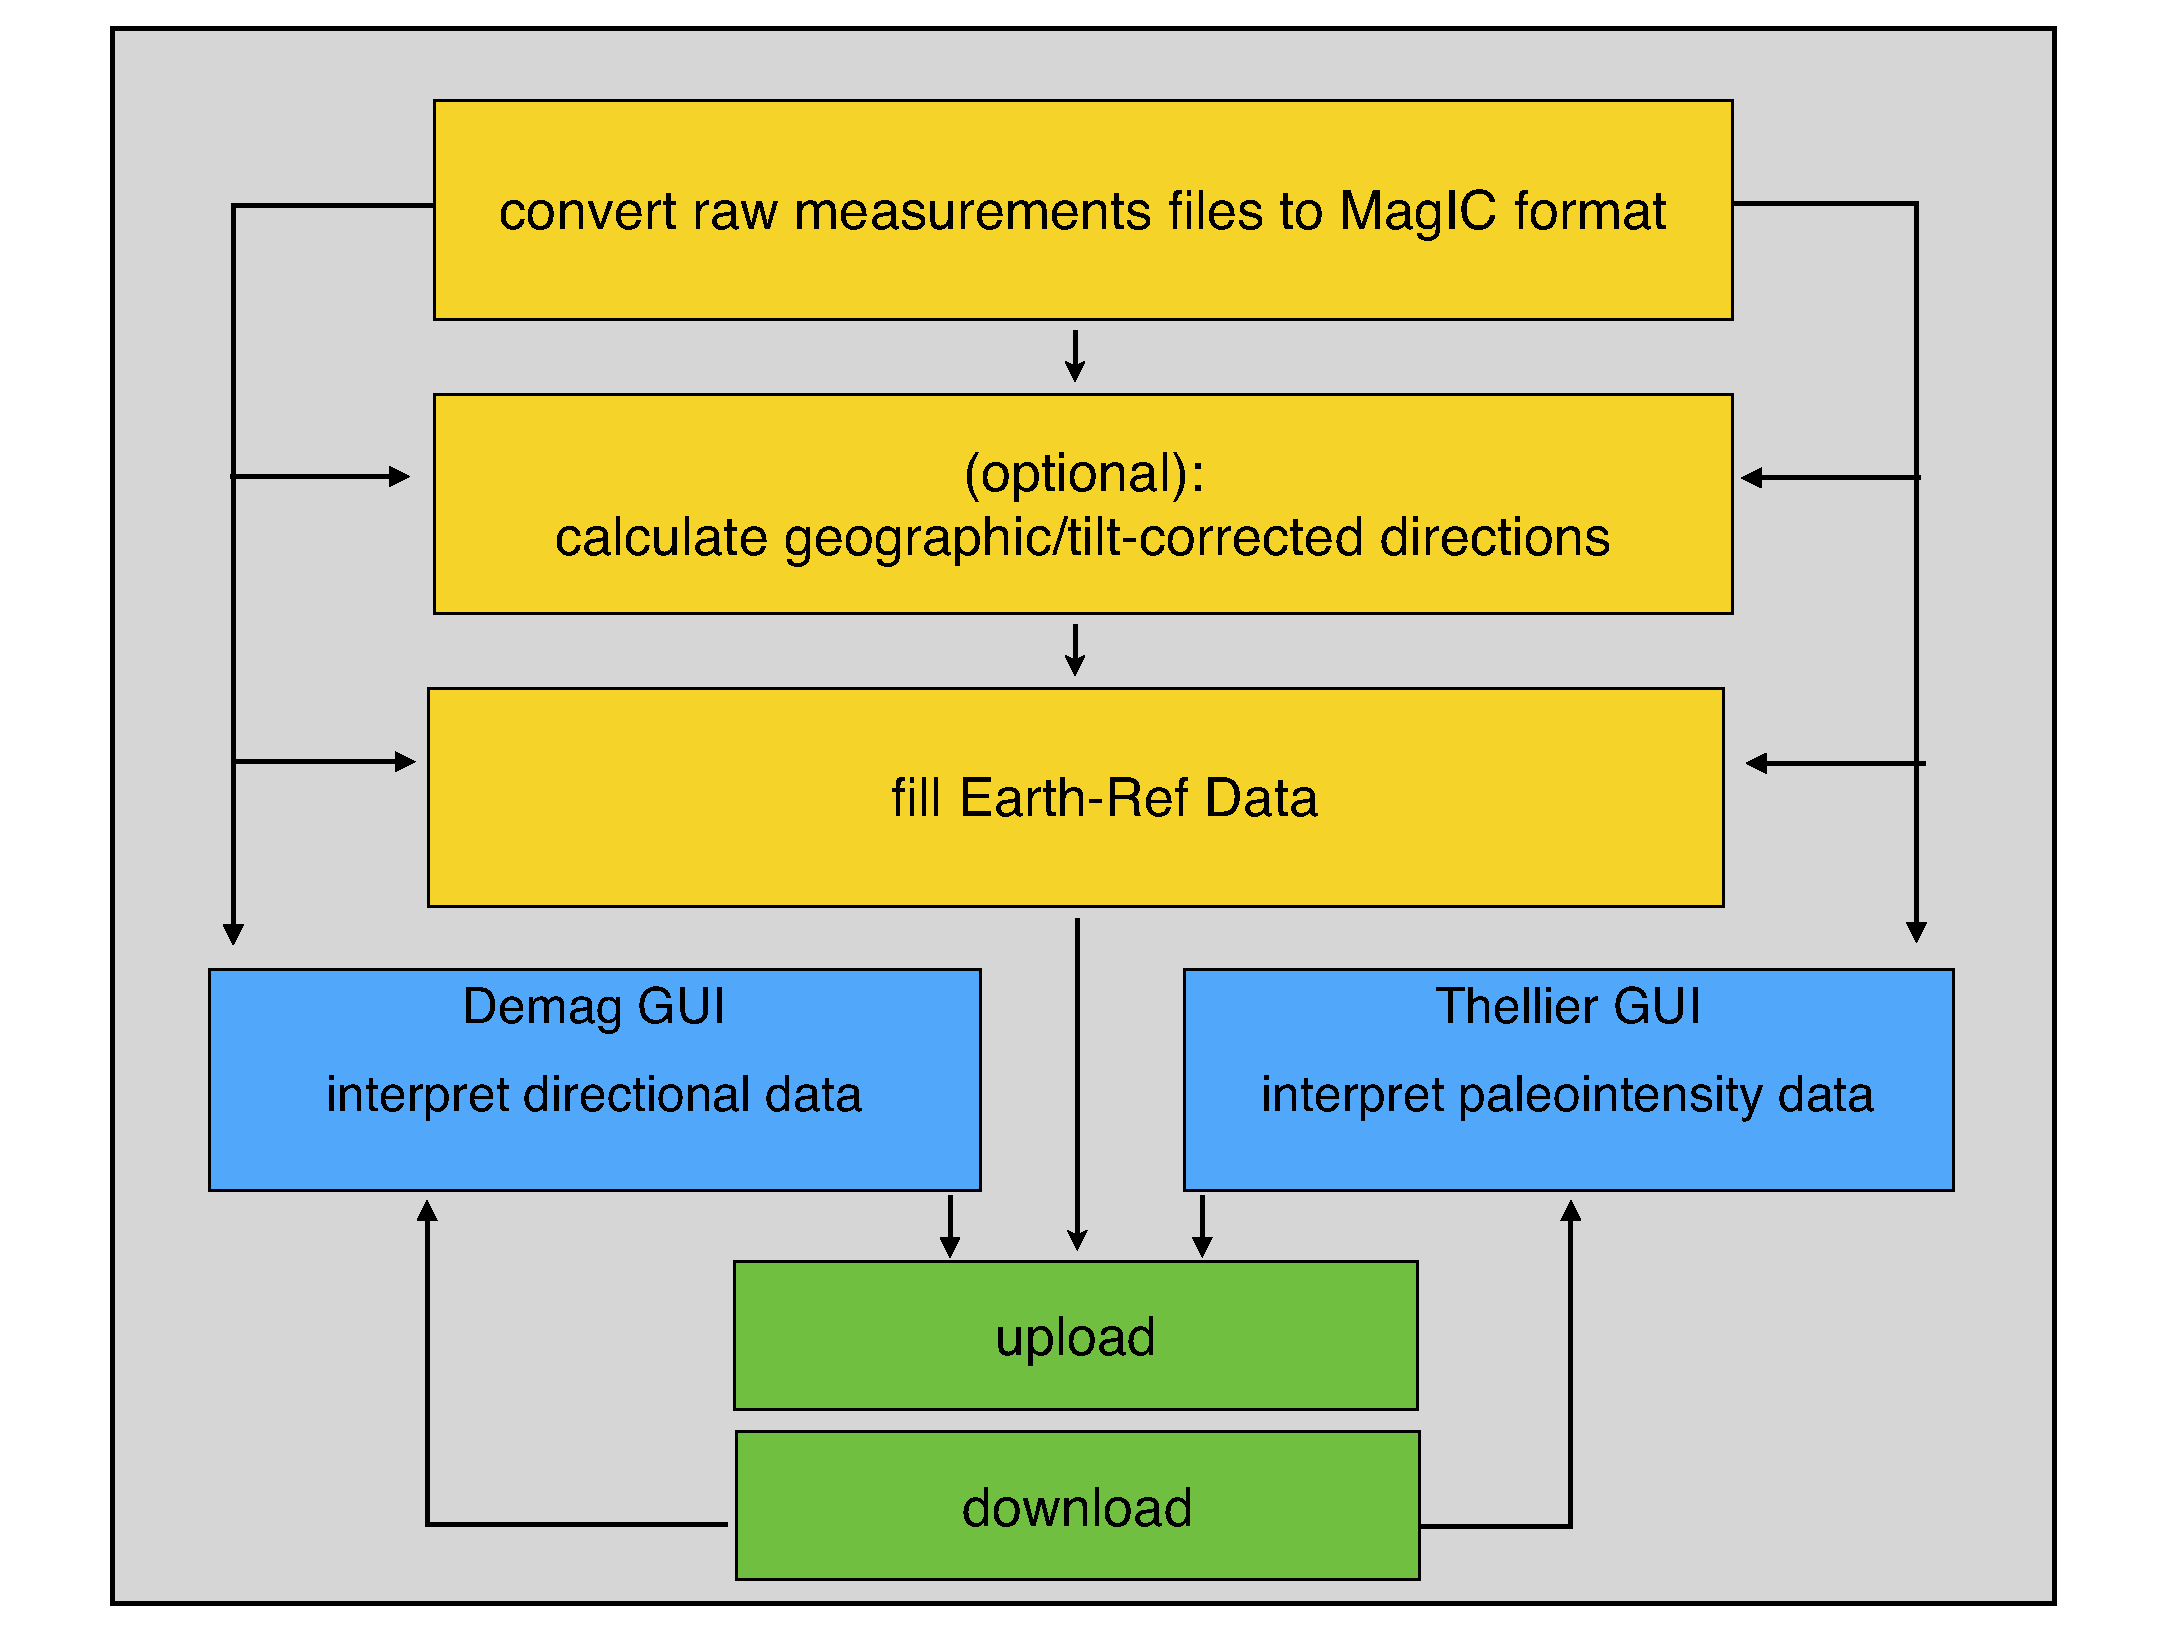
\includegraphics[width=15cm]{EPSfiles/FigQkMagicFlow.eps}

\begin{enumerate}
\item Follow the steps in the \href{#quick_start}{Installing PmagPy} section.

\customlink{Project_Directory}

\item  When you invoke {\bf Pmag GUI}, the first step is to change directories into a  `Project Directory'. For each study, create a directory with a name that relates to that study. Here we will call it {\it ThisProject}.  This is where you will collect and process all the rock and paleomagnetic data for a given study, usually a publication. The project directory name should have NO SPACES and be placed on the hard drive in a place that has NO spaces in the path. Under certain Windows versions, this means you should not use your home directory, but create a directory called for example: D:$\backslash$MyPmagProjects and put {\it ThisProject} there.
%
%Inside the  {\it ThisProject} directory, create two additional directories: {\it MyFiles} and {\it MagIC}. All the files that you want to convert to the MagIC format should be placed in {\it MyFiles}.  The {\it Project Directory} that {\bf Pmag GUI} seeks is that {\it MagIC} directory.
%
%Your Directory tree might look like this now:
%
%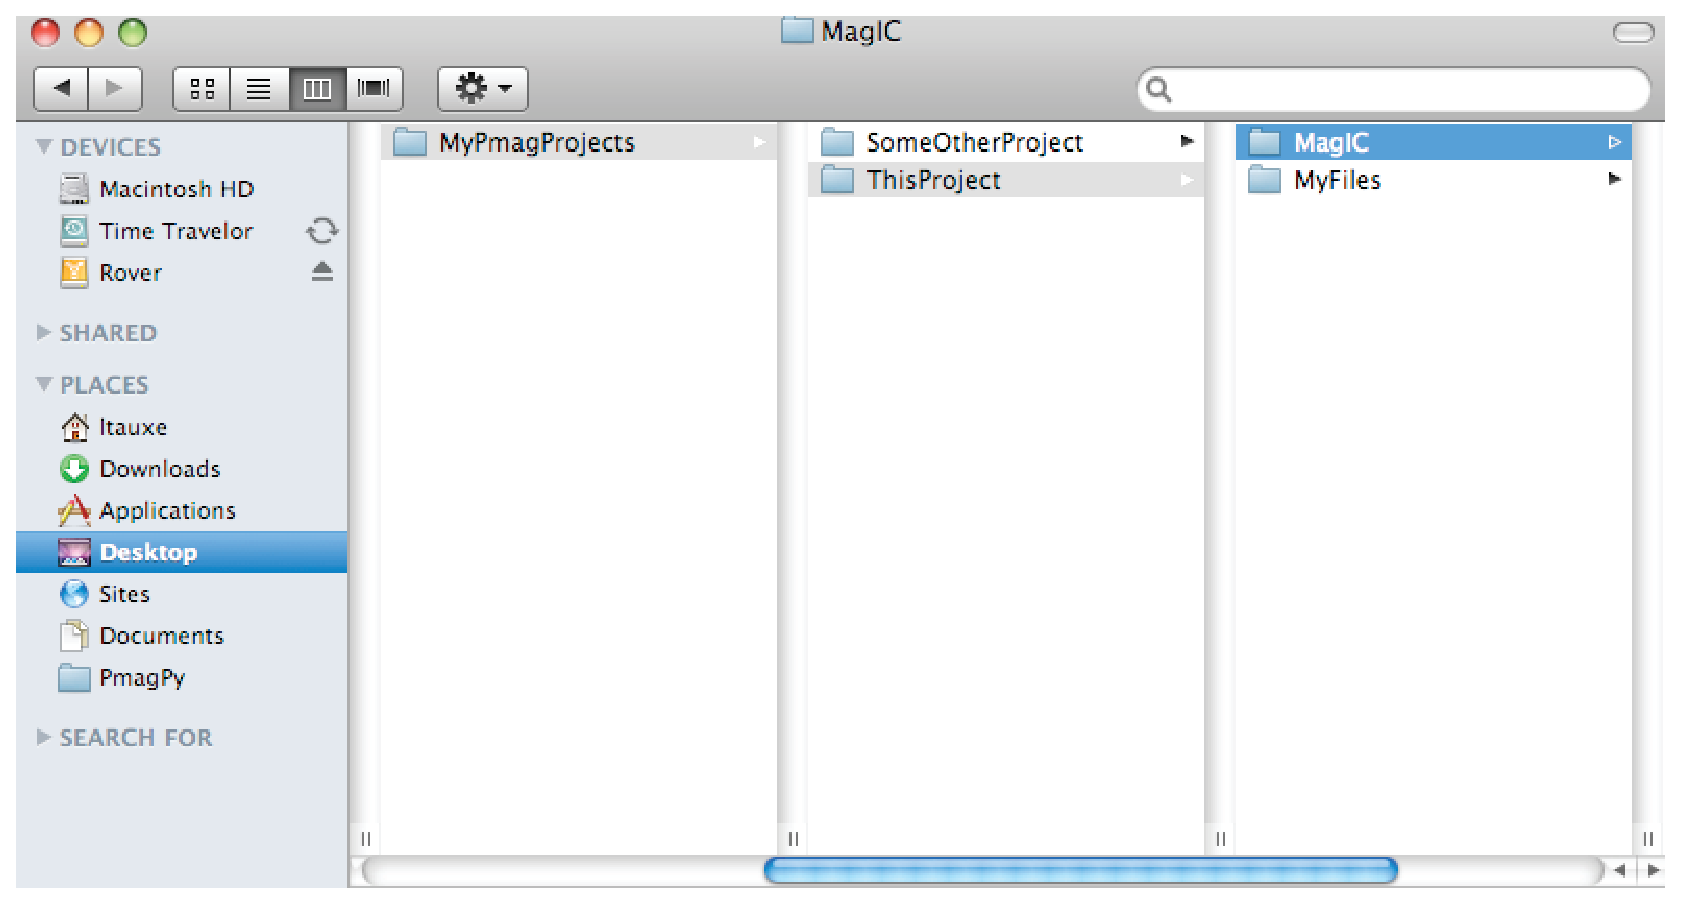
\includegraphics[width=15cm]{EPSfiles/ProjectDirectory.eps}


 \item \textbf{copy example files:}  In the \href{#Datafiles}{ Datafiles } folder you will find a subfolder named {\it Pmag\_GUI}. Copy the contents of the  \href{#Project_Directory}{\it ThisProject} directory  into  your  own \href{#Project_Directory}{Project Directory} folder.
 \item Start Pmag GUI either by typing {\bf pmag\_gui.py} on your \href{#command_line}{command line}, or (if you have the \href{#standalone}{standalone}), by double-clicking the Pmag GUI icon on your Desktop.
 \item Change directories by clicking  on the ``change dir'' button and select your own {\it ThisProject} directory.
 \end{enumerate}

 \customlink{convert2magic}

\section{Converting magnetometer files to MagIC format}
\begin{itemize}
\item {\bf Pmag GUI} allows for converting many different laboratory formats.  For the complete set of instructions, see the section on \href{#magnetometer_files}{Supported Rock Magnetometer files}.   For this example, we will use a `generic' file format.
%rshaar% In the {\it MyFiles} folder there are  files containing AF, Thermal, and Thellier measurement data of samples from location Snake River (lava flow site). All samples are from site sr01. The measurement data are arranged in the generic format.
An example for a generic file format is shown here:

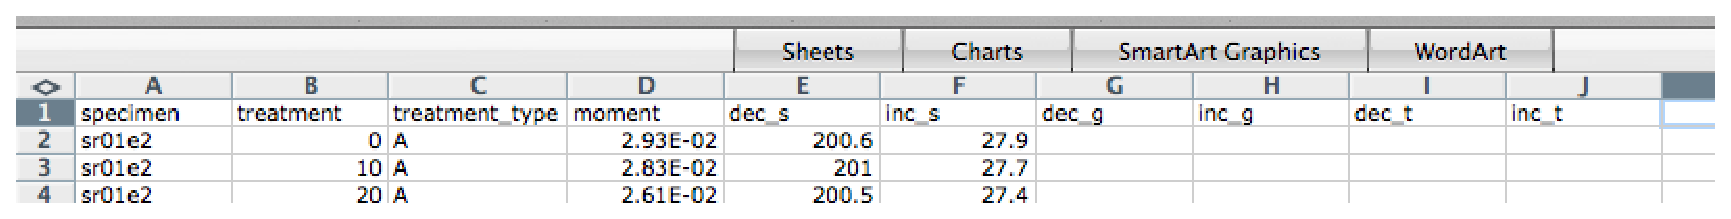
\includegraphics[width=15cm]{EPSfiles/FigGenericFormat.eps}

To learn what all the column headers mean look at the documentation for \href{#generic_magic.py}{generic\_magic.py}.

%\item Locate the {\it MyFiles} folder in  the {\it Datafiles} subdirectory named {\it Pmag GUI} and copy the contents to your own {\it MyFiles} directory.
%
%\includegraphics[width=15cm]{EPSfiles/FigMyFiles.eps}

%\item Run the program: Open up a terminal window (Mac) or command prompt (Windows) and type pmag_gui.py on the command line. In the Pmag GUI main panel press the Õchange dirÕ button. Select the MagIC directory in ThisProject when prompted.

\item In your  \href{#Project_Directory}{\it ThisProject} directory  there are three files with AF, Thermal, and Thellier measurement data of specimens from site sr01 (a lava flow site) of \cite{tauxe04b}.  There is also a file with sample orientation, location and other metadata typical for a paleomagnetic study.
\item Press the [Convert magnetometer files to MagIC format] button. If no menu pops up or the window is blank, click on the Python icon  (the little space ship) on your dock. You should see a dialog window will appear with different file formats:

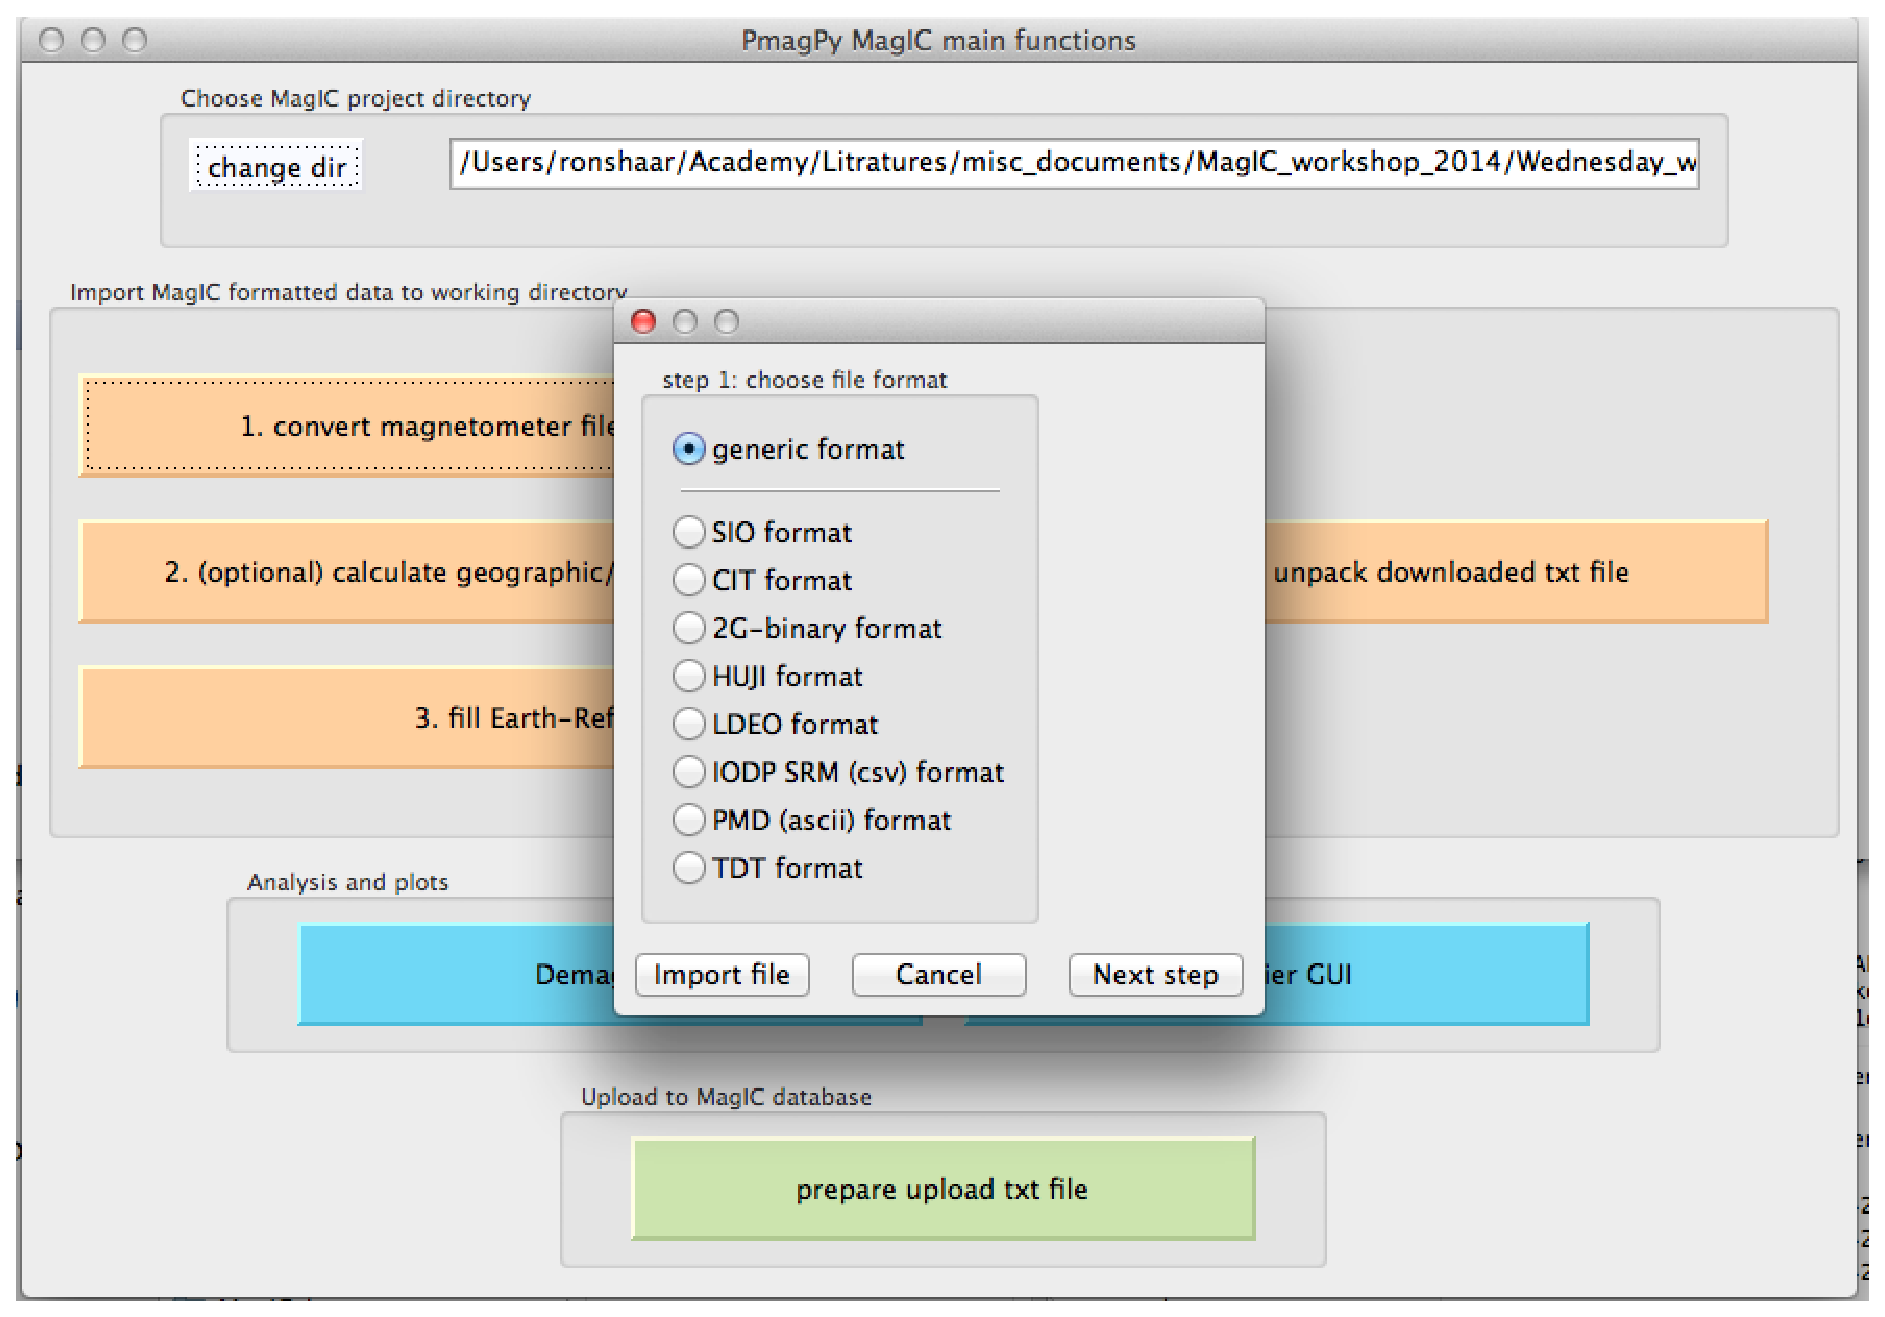
\includegraphics[width=15cm]{EPSfiles/FigChooseFile.eps}

\item  Click on  `generic format'  and press the  [import file] button.  A new dialog box will appear. For more details click on the [help] button.
\item  In the dialog box, click on the [Add] button and choose one of the measurements files.
\item  Optional: Insert your EarthRef user name.
\item Choose your experiment type from the dropdown list.

\item Choose specimen-sample naming convention.  In this example, specimen sr01a1 belongs to sample sr01a so the specimen-sample naming convention is  `no. of terminal characters ' and the delimiter/number field is `1' ).
\item Choose sample-site naming convention.  In this example, sample sr01a belongs to site sr01 so the sample-site naming convention is  `no. of terminal characters' with a delimiter/number of  `1'.
\item  Fill in the \href{#MagICDatabase}{EarthRef Location Name}  for this project .  For this project, it is ``Snake River''.
\customlink{location_name}

\item Note:  a location is a stratigraphic section,  a sampling region,  an drill core, and so on.  MagIC doesn't really care what your location name is, but use the same location name every time you are asked for it, because it really ties your dataset together and is required within the data model.

Your dialog boxes should look like this for the AF and thermal data:

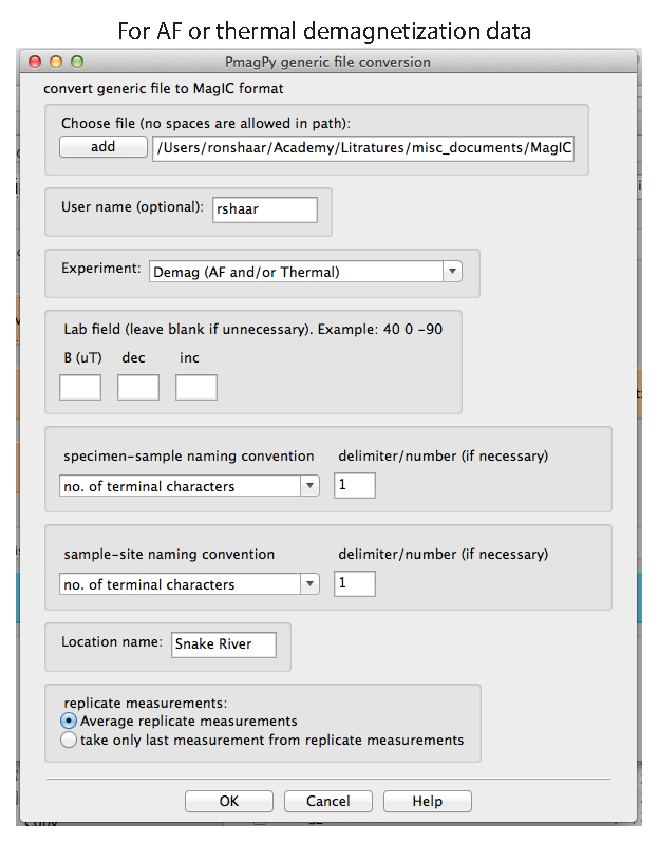
\includegraphics[width=15cm]{EPSfiles/FigConvertGenericA.eps}

and like this for the  paleointensity data.  For paleointensity data, you must also supply the lab field in micro tesla (40) and orientation relative to sample's X direction:  0 90.

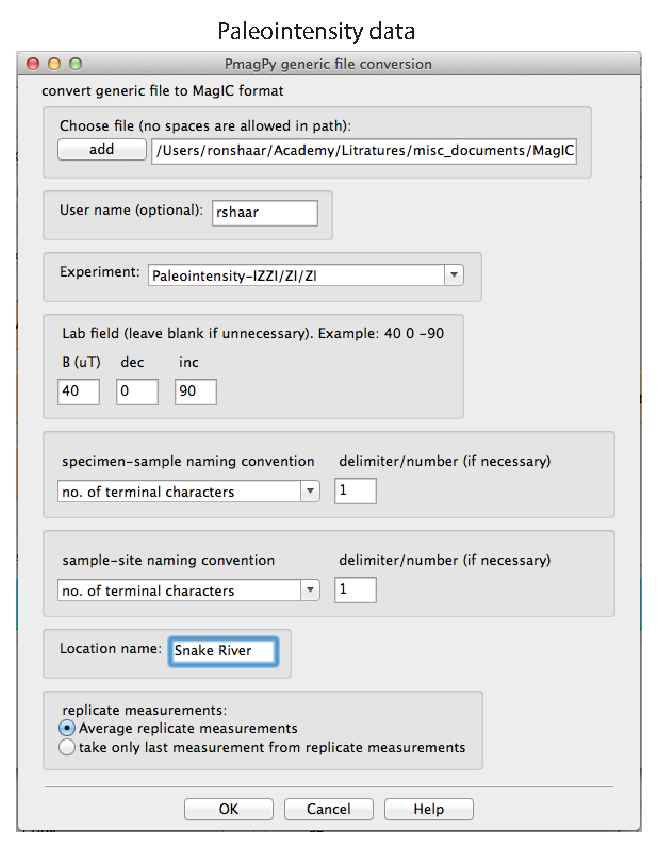
\includegraphics[width=15cm]{EPSfiles/FigConvertGenericB.eps}

\item Press OK to create a new MagIC measurement file, which is saved in your \href{#Project_Directory}{\it ThisProject} directory.


\customlink{Combine}

\item After converting all files to MagIC format, press the [Next Step] button in the `convert magnetometer files' dialog box. All files with the .magic suffix will be added to the list.  [You can edit the list by deleting unwanted files or adding additional MagIC formatted files.]   You should see a list of the three magic files:

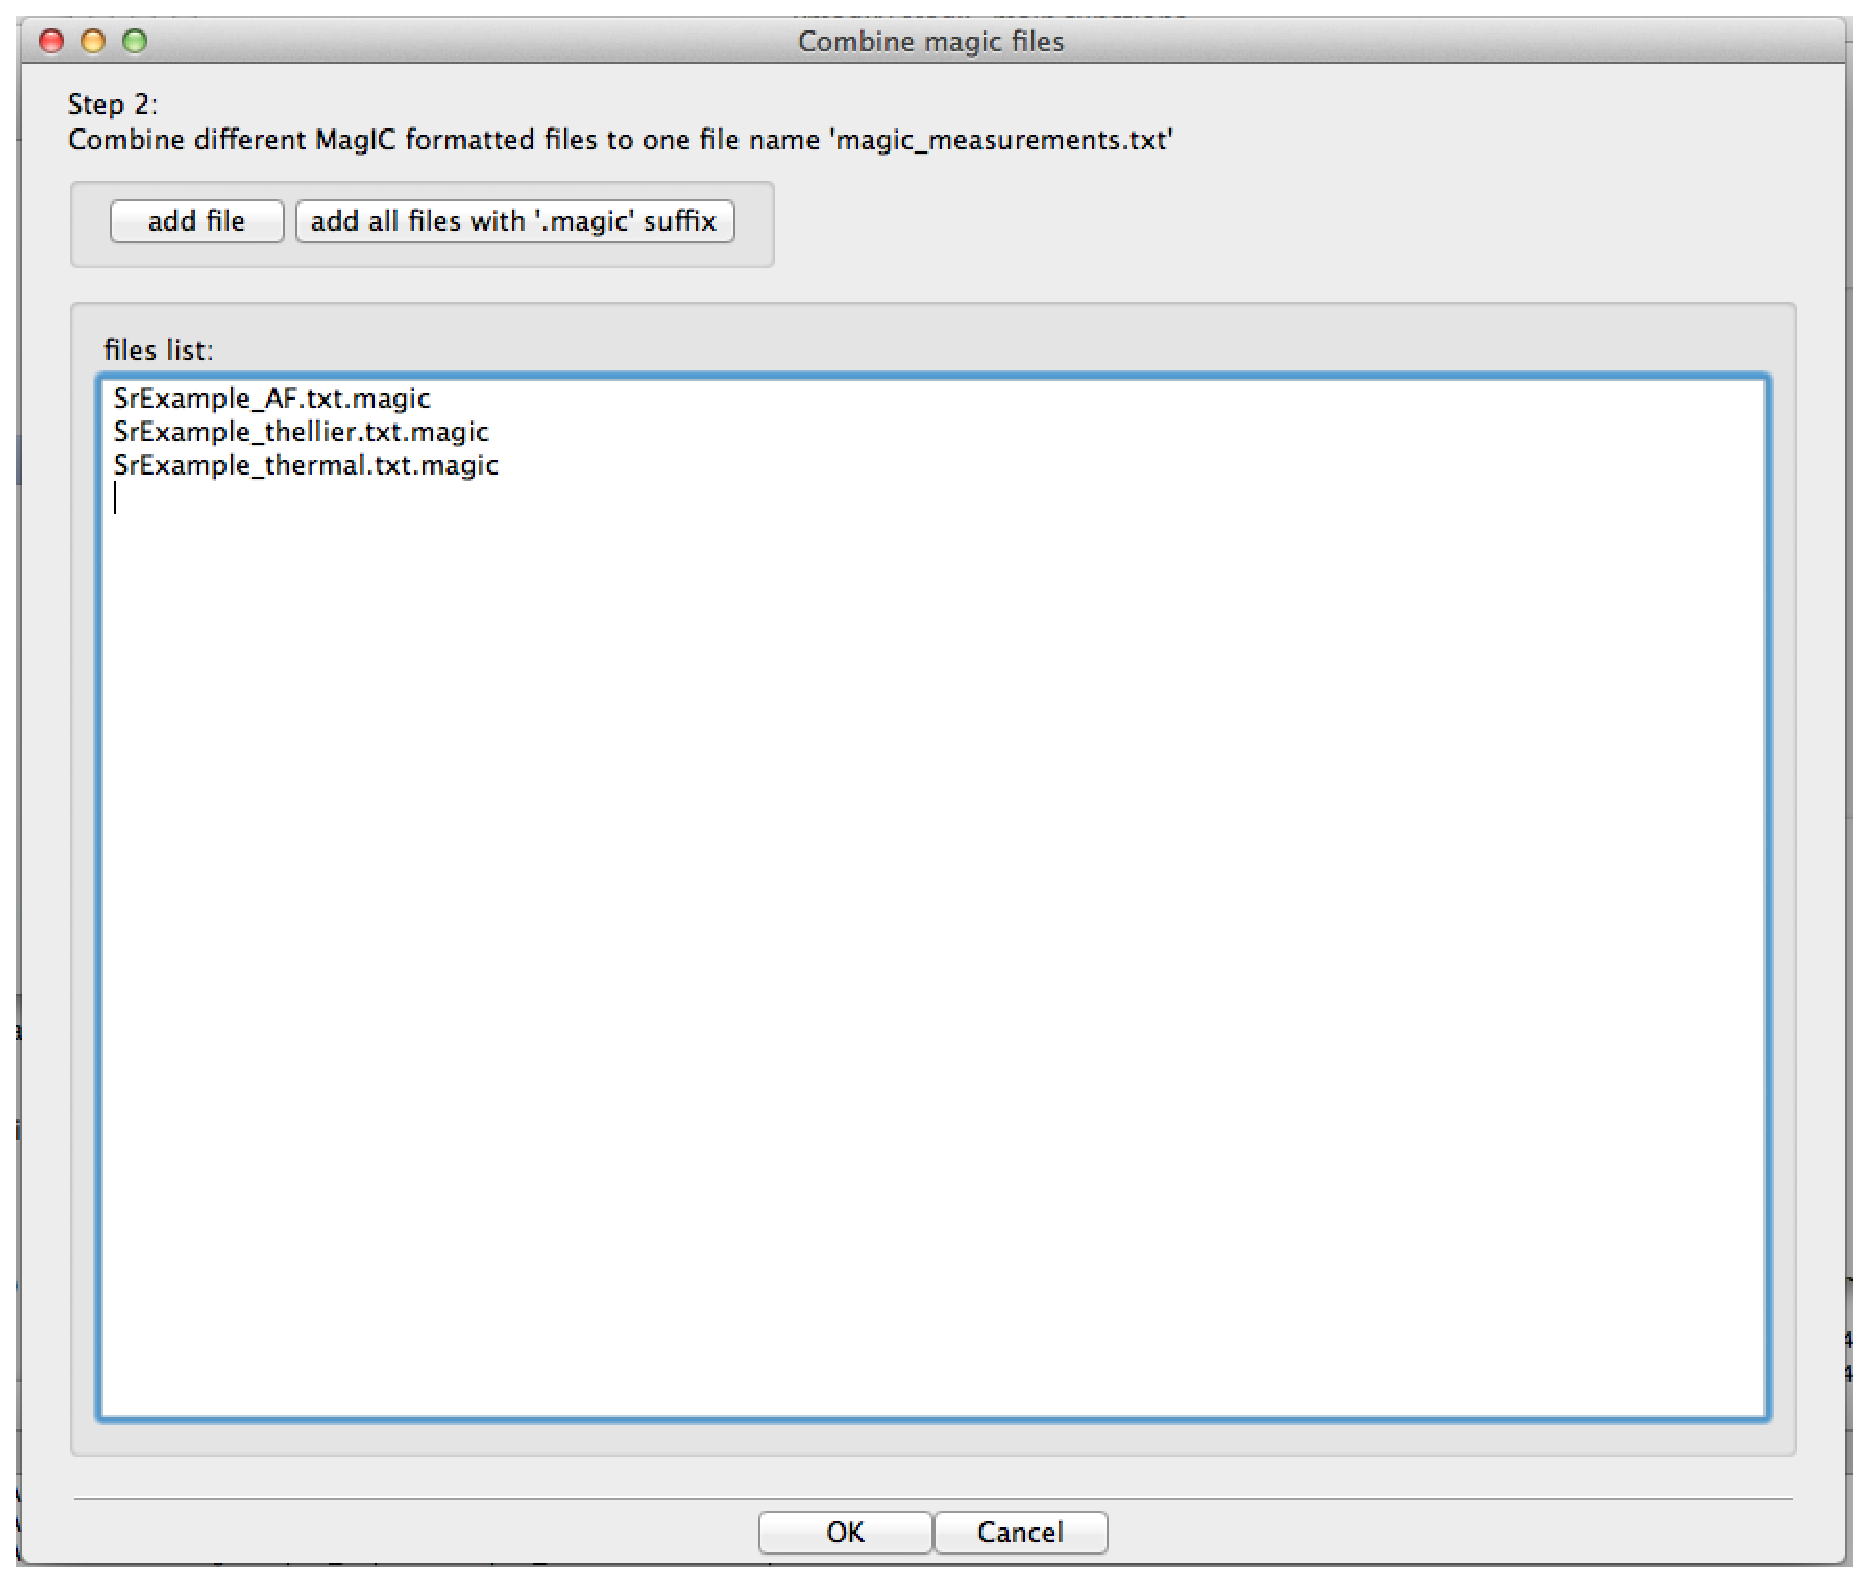
\includegraphics[width=15cm]{EPSfiles/FigCombineMagic.eps}

\item Click the OK button. The three files will be combined to a single file,  named {\it magic\_measurements.txt} and also stored  in your \href{#Project_Directory}{\it ThisProject} directory.
\end{itemize}

\customlink{orient}

\section{Optional: Calculate geographic / tilt-corrected direction}
\begin{itemize}
\item {\bf Pmag GUI} provides an optional tool for calculating geographic and tilt-corrected directions if those directions were not part of the original data files. To use this tool click on the button labeled `calculate geographic/tilt-corrected directions'.

\item An empty template of a file named ”SrExample\_orient.txt• was created in the MagIC Project Directory. This file is displayed in a Python window. You can fill in  this file manually using the Python window or \href{#field_info}{with with a spreadsheet program} (recommended). The empty template has now only the sample names derived from your measurement files, using the naming rules that you chose.
\item To see an example of a filled in one, pull down the menu bar [file] $\rightarrow$  [open orientation file] and  choose the file SrExample\_orient.txt from {\it MyFiles} folder.
\item Choose from the menu bar [file] $\rightarrow$ [Save orientation file].
\item Choose from the menu bar [file] $\rightarrow$ [Calculate sample orientation].
\item Fill in the dialog box like this:

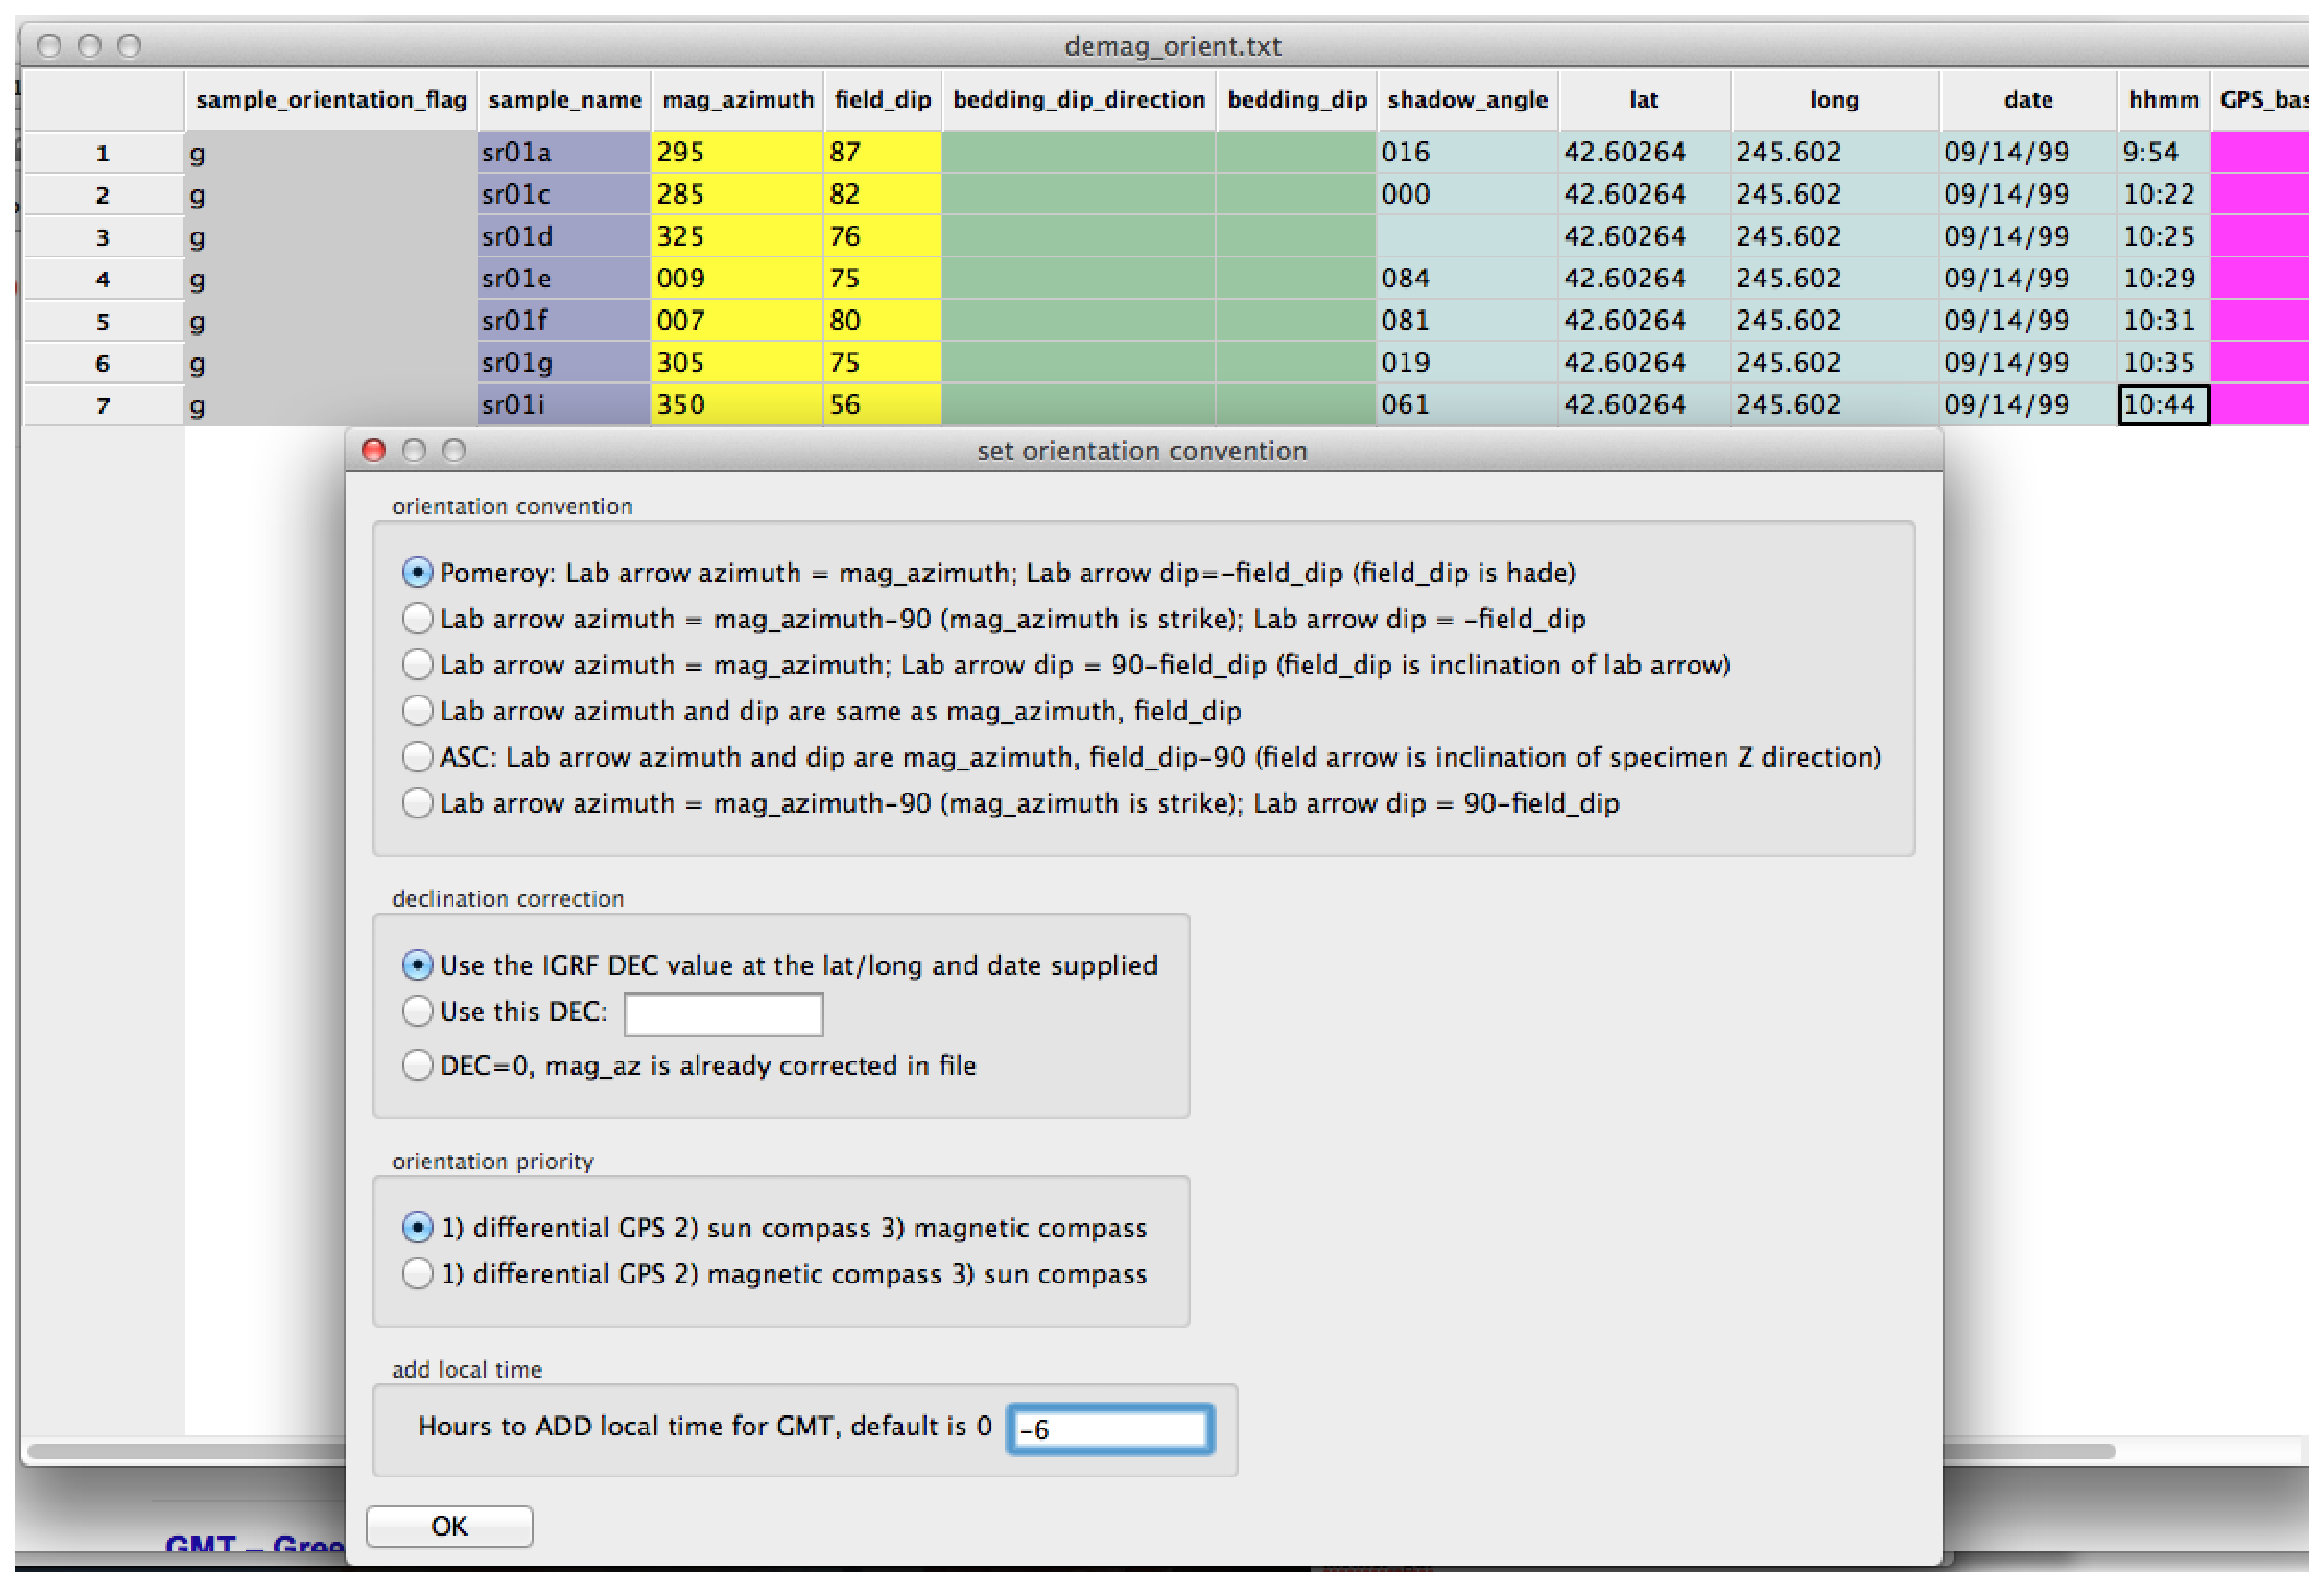
\includegraphics[width=15cm]{EPSfiles/FigDemagOrient.eps}

\begin{itemize}
\item Orientation convention :Pomeroy.
\item Declination correction: Use the IGRF.
\item  Orientation priority: \#1.
\item Put in the number of hours to SUBTRACT from the local time to get to Greenwich Mean Time: -6. [Local time was 6 hours behind GMT for this example.]
\item press the OK button.
\end{itemize}
\item In the next dialog window add the additional information:
\end{itemize}

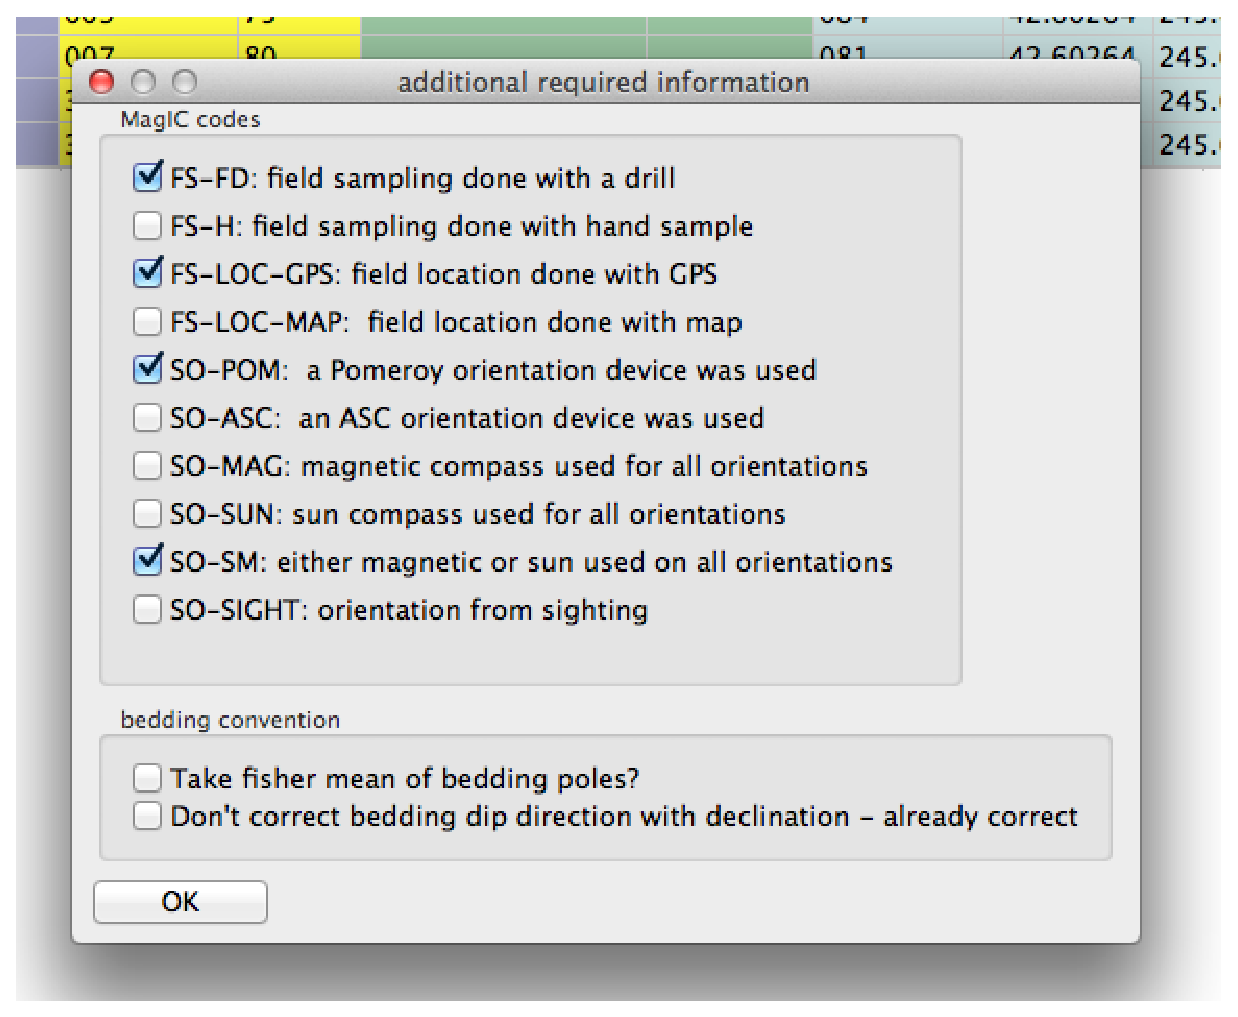
\includegraphics[width=15cm]{EPSfiles/FigOrientMagicCodes.eps}

\section{Filling in the EarthRef data}

Filling in the Earth Ref data is a critical part of building a MagIC Project Directory. The Earth-Ref data relevant to this example are arranged in five er\_* tables: er\_specimens, er\_samples, er\_sites, er\_locations, er\_ages. To complete the  ER data, click the button, and follow the directions in the help window in order:

\begin{itemize}
\item Step 0: Choose the appropriate headers for each of your er\_* tables.  Required headers (or headers already present in your er\_* tables) show up in the top box, optional headers in the bottom.  Once you have added all needed headers, click the OK button to proceed to the next step.

 \includegraphics[width=30cm]{EPSfiles/FigErMagicStep0.eps}

 \item The next six steps contain editable grids.  For many columns, you can edit using drop-down menus that provide \href{http://earthref.org/MAGIC/shortlists.htm}{controlled vocabularies}.  For others, you must manually enter data into the cell.  A single left click will bring up a drop-down menu; a double-left click will call up the cell editor.  With both types of data entry, it is possible to select a single value for the entire column. Simply click on the column label.  If that column has a drop-down menu, you can then click on any cell in the column, the appropriate menu will pop up, and the value you select will propagate throughout the column.  Edits in that column will continue to be global until you select another column to edit or you de-select the column by clicking on the column label again.  If you select a column that does not have a drop-down menu, a text entry dialog will pop up, and the value you provide will be applied to the column.

 \item Step 1: Update the relationship between specimens and samples.  You may not rename specimens, but you may reassign them to a different sample.  It is also possible to add additional samples, using the 'Add new sample' button.  Note that specimen\_type, specimen\_lithology, and specimen\_class columns do not show up.  They will propagate down when you select sample\_type, sample\_lithology, and sample\_class in step 4.

 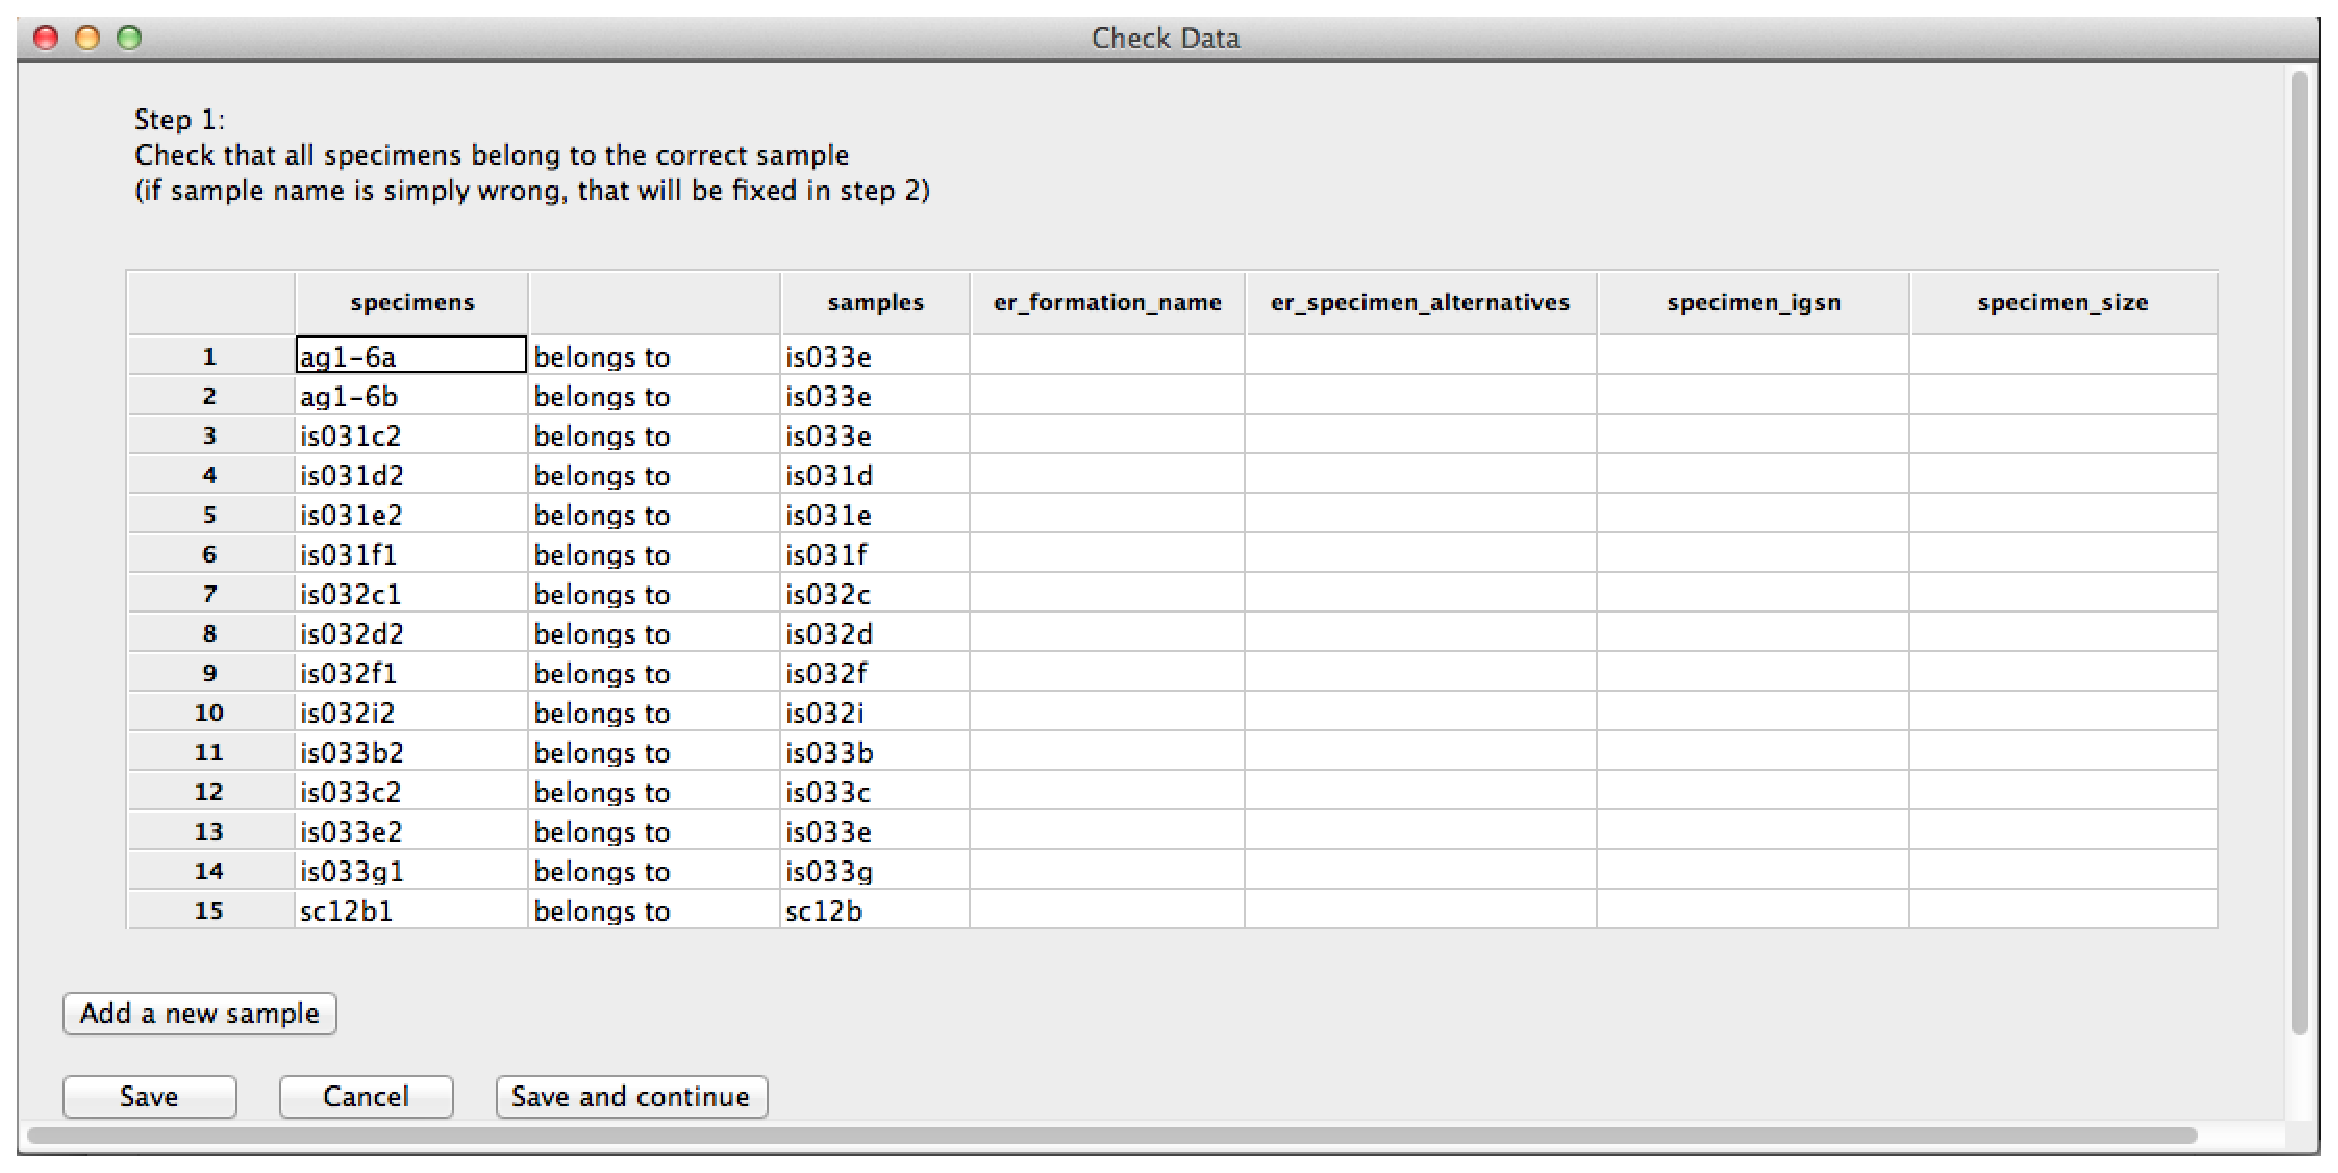
\includegraphics[width=16cm] {EPSfiles/FigErMagicStep1.eps}

\item Step 2:  Update the relationship between samples and sites.  You may rename samples, or you can reassign them to a different site.  You can also add additional sites using the ``Add a new site`` button.  You will be able to update other columns in the er\_samples file in step 4.

 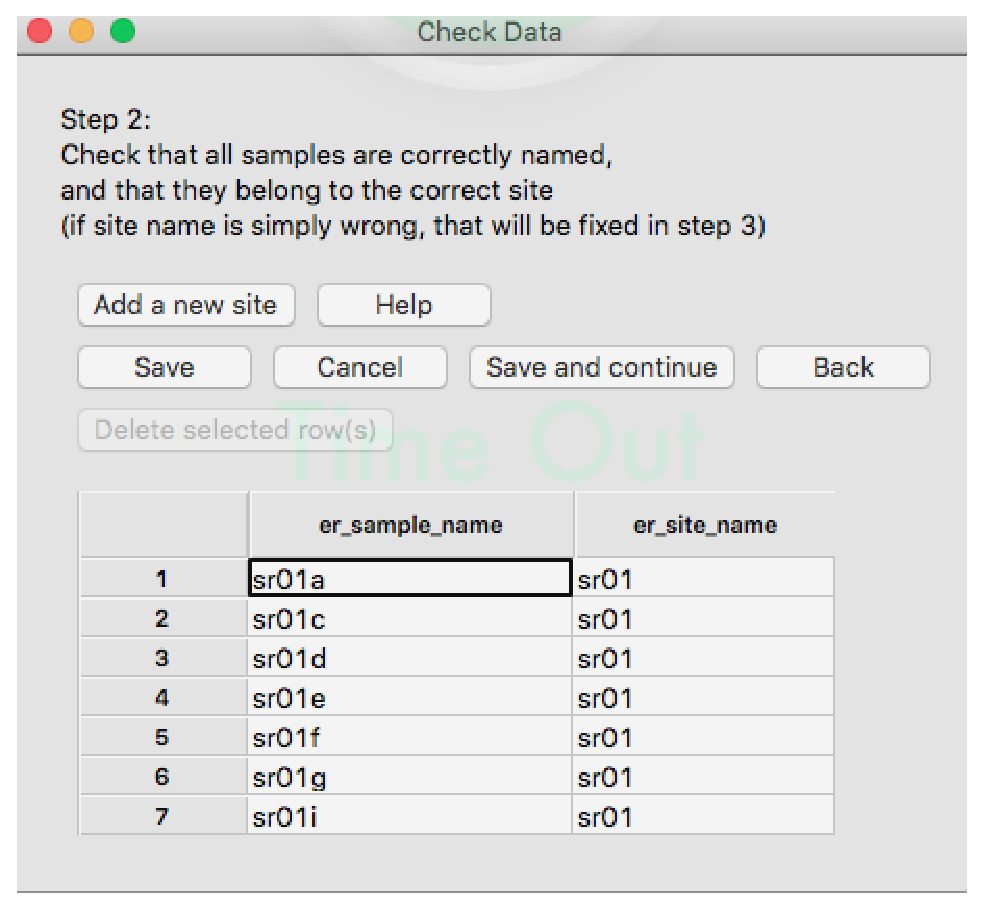
\includegraphics[width=16cm] {EPSfiles/FigErMagicStep2.eps}

\item Step 3: Update the relationship between sites and locations.  You may rename sites, or you can reassign them to a different location.  You can add additional locations using the ``Add a new location'' button.  You must choose a legal entry from the \href{http://earthref.org/MAGIC/shortlists.htm}{controlled vocabularies} for the following headers: ``site\_class'', ``site\_lithology'', ``site\_type''. You may combine more than one controlled vocabulary by making them a colon delimited list.  If you select a value in these categories: class, lithology, type, longitude, or latitude, the values will propagate to the samples table.  In this example,  site\_class=Extrusive:Igneous; site\_lithology=Basaltic Lava; site\_type=Lava Flow

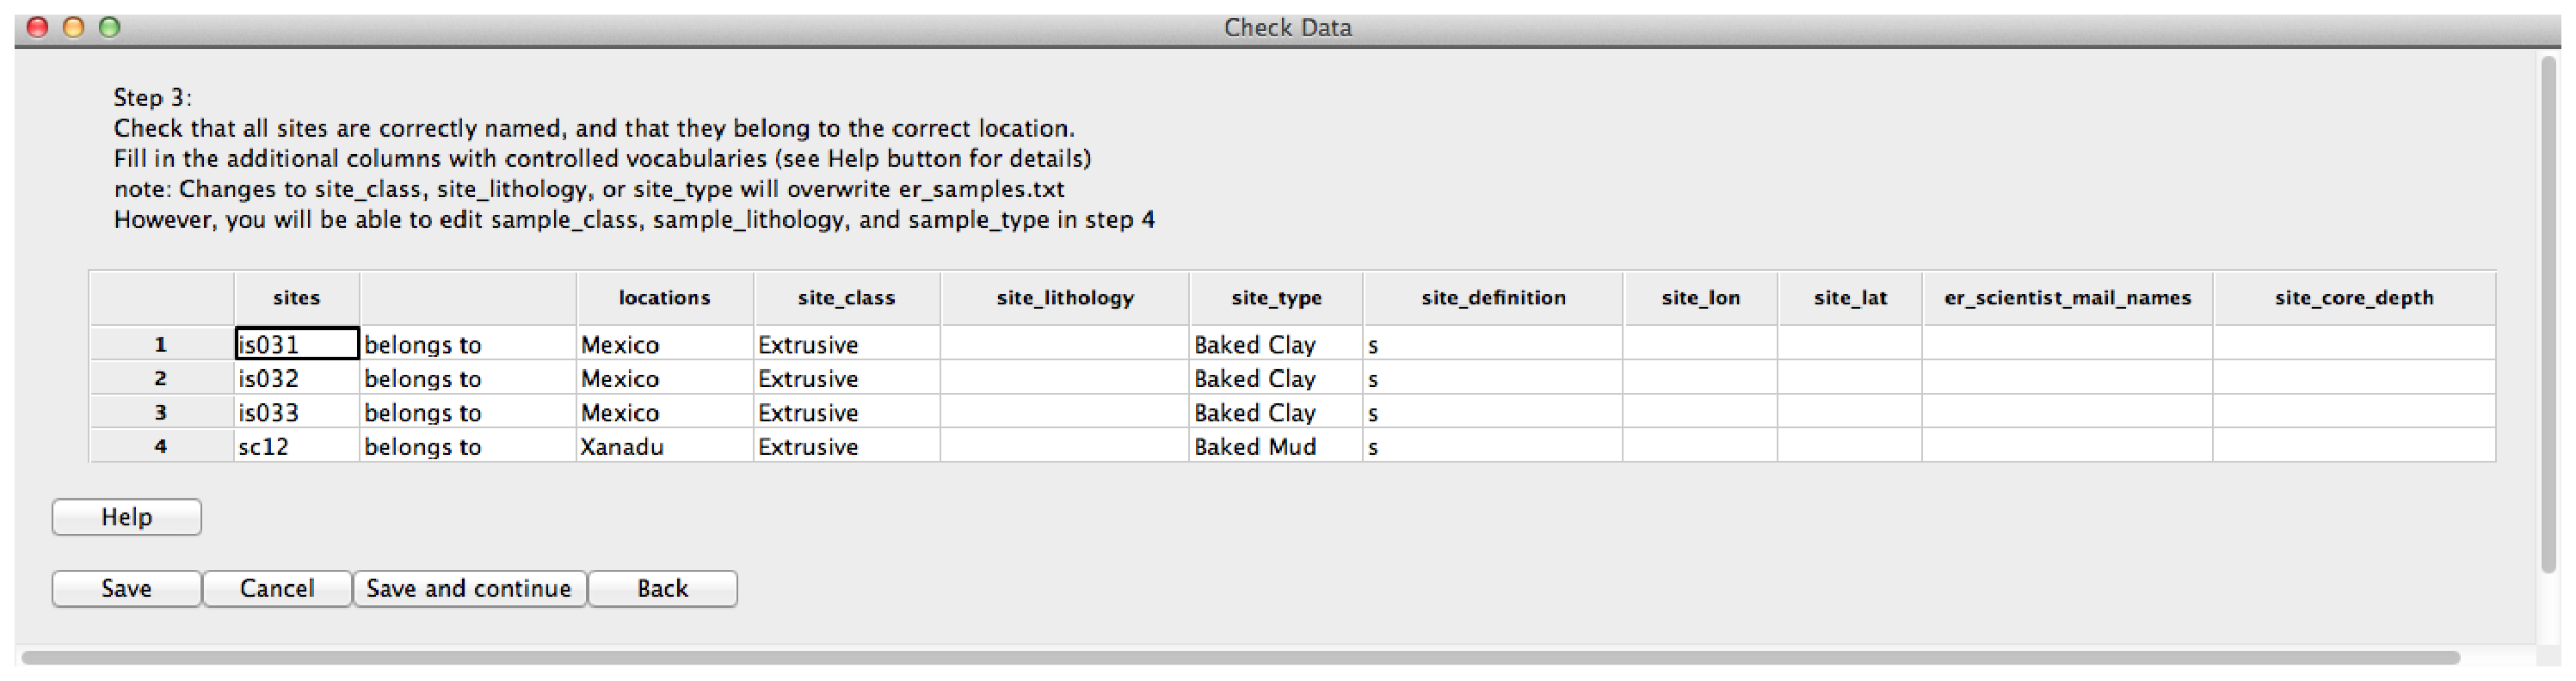
\includegraphics[width=32cm] {EPSfiles/FigErMagicStep3.eps}

\item Step 4: Some data from sites in Step 3 have propagated into the samples table.  You may update and fill in all columns in the samples table here.

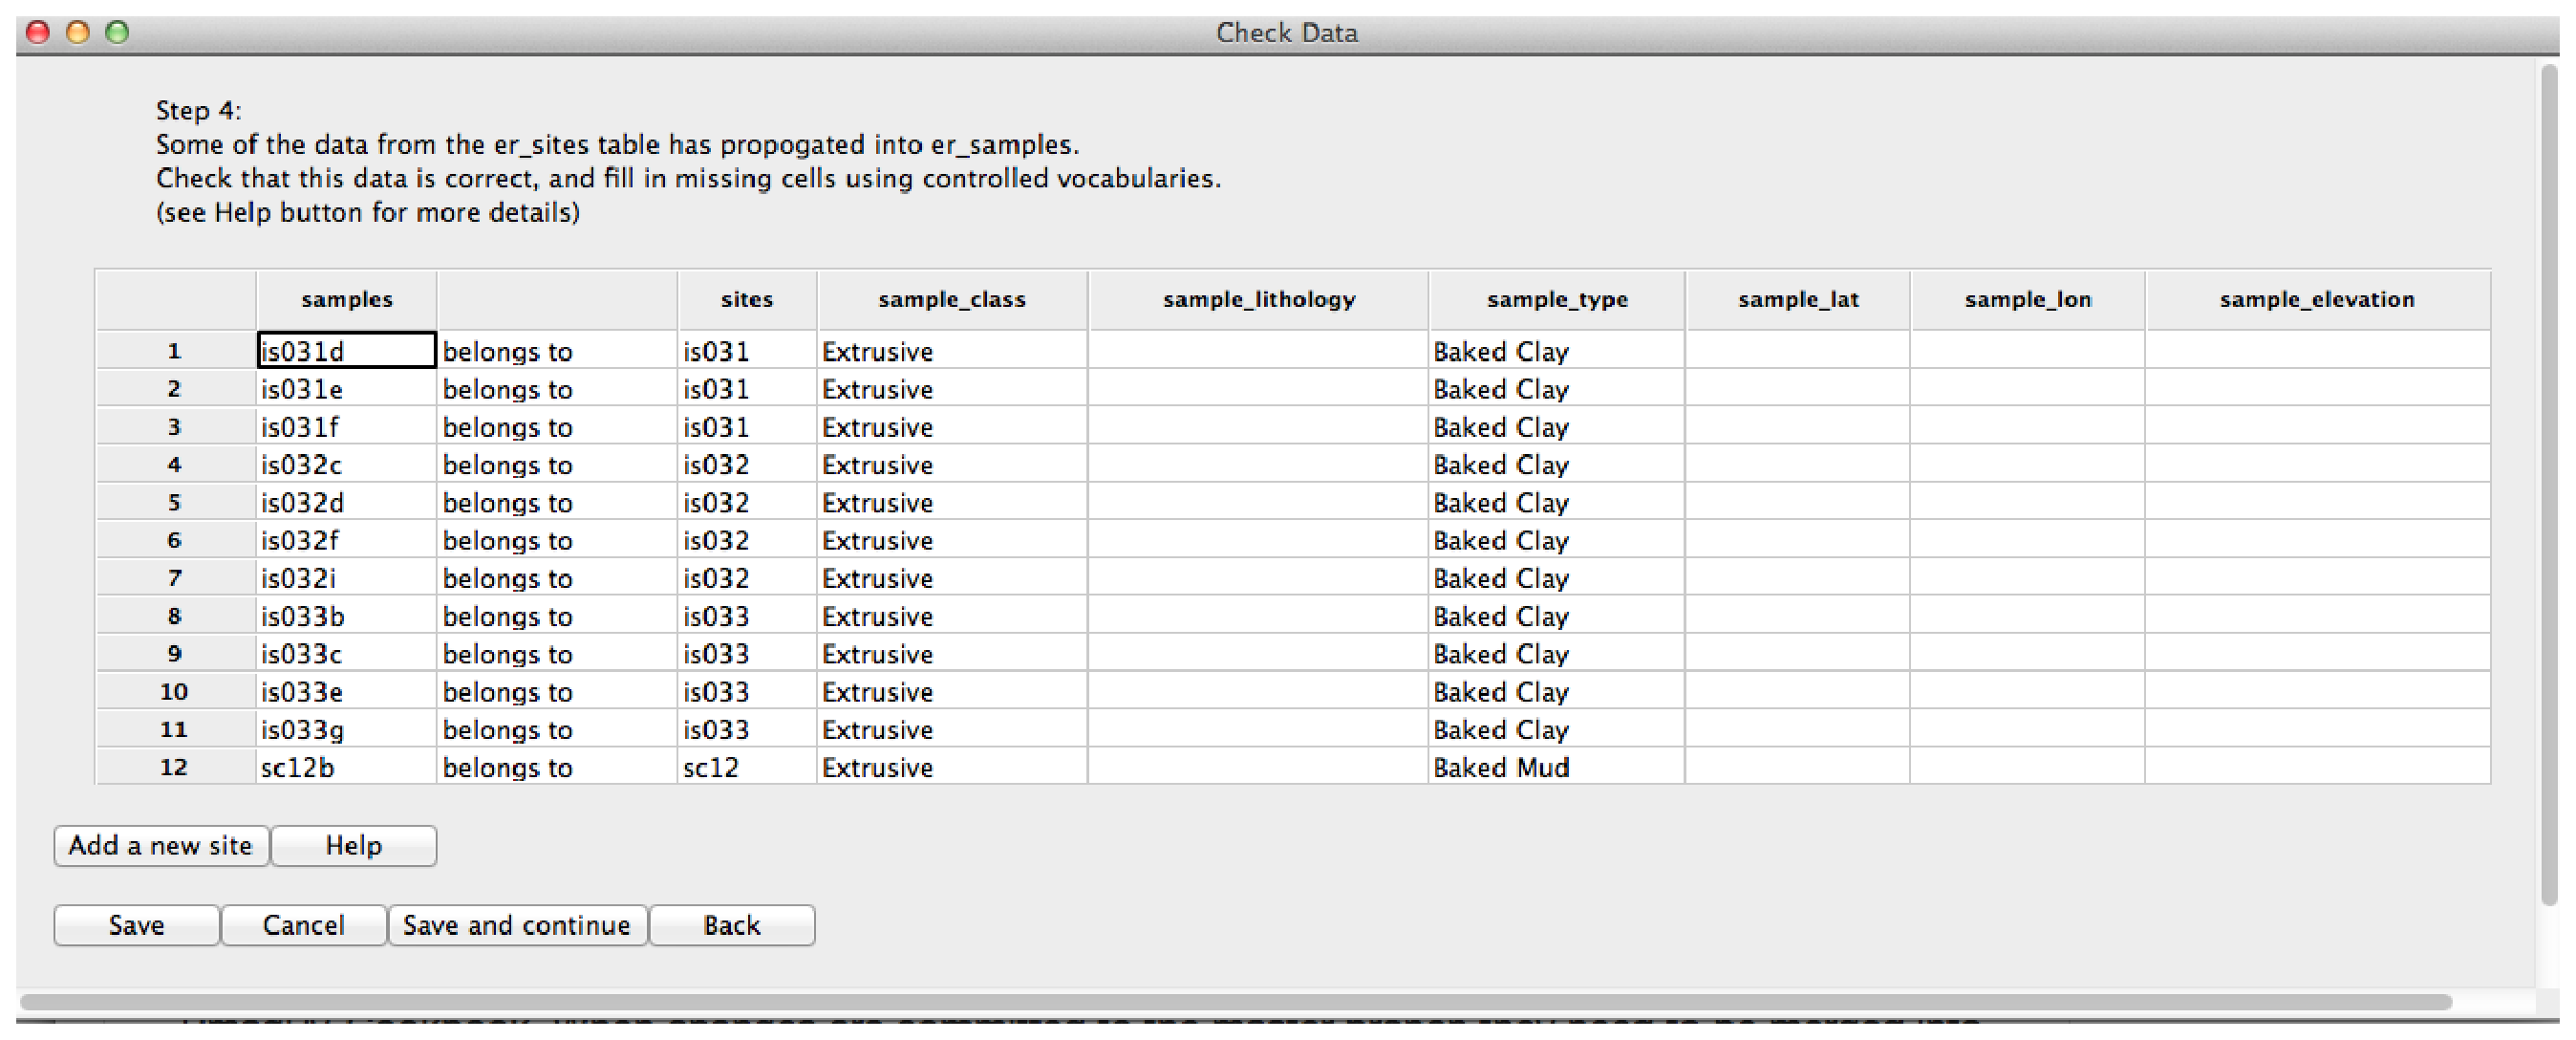
\includegraphics[width=32cm] {EPSfiles/FigErMagicStep4.eps}

\item Step 5: Fill in information for locations.  If you have provided site latitudes and longitudes, the columns for beginning and ending latitudes and longitudes should be filled in already. You must choose a legal entry from the \href{http://earthref.org/MAGIC/shortlists.htm}{controlled vocabularies} for the  ``location\_type''. In this example: location\_type = outcrop.

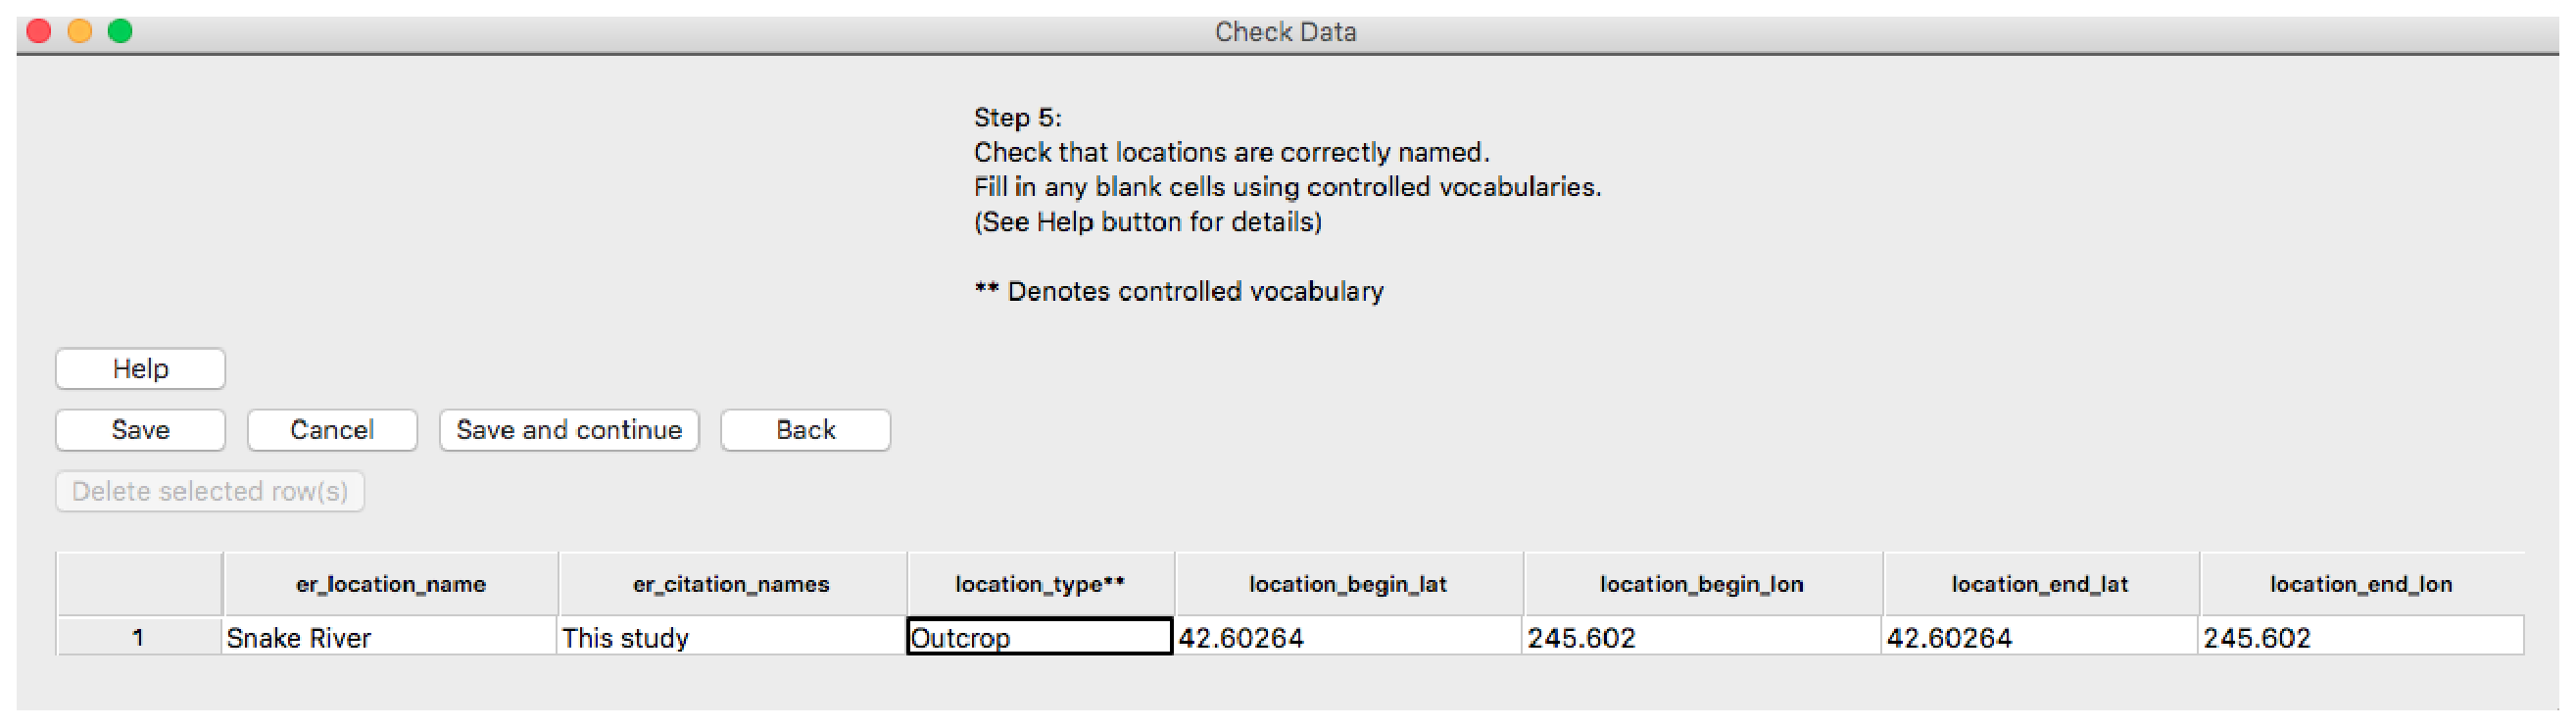
\includegraphics[width=32cm] {EPSfiles/FigErMagicStep5.eps}

\item Step 6: Fill in columns with any necessary information.   In this example, age=3.4; age\_sigma=0.03 (not a default header); age\_unit=Ma (from controlled vocabularies), magic\_method\_codes  = GM-ARAR-AP (from \href{http://earthref.org/MAGIC/shortlists.htm}{controlled vocabularies}). It means ``40Ar/39Ar age determination: Age plateau.''

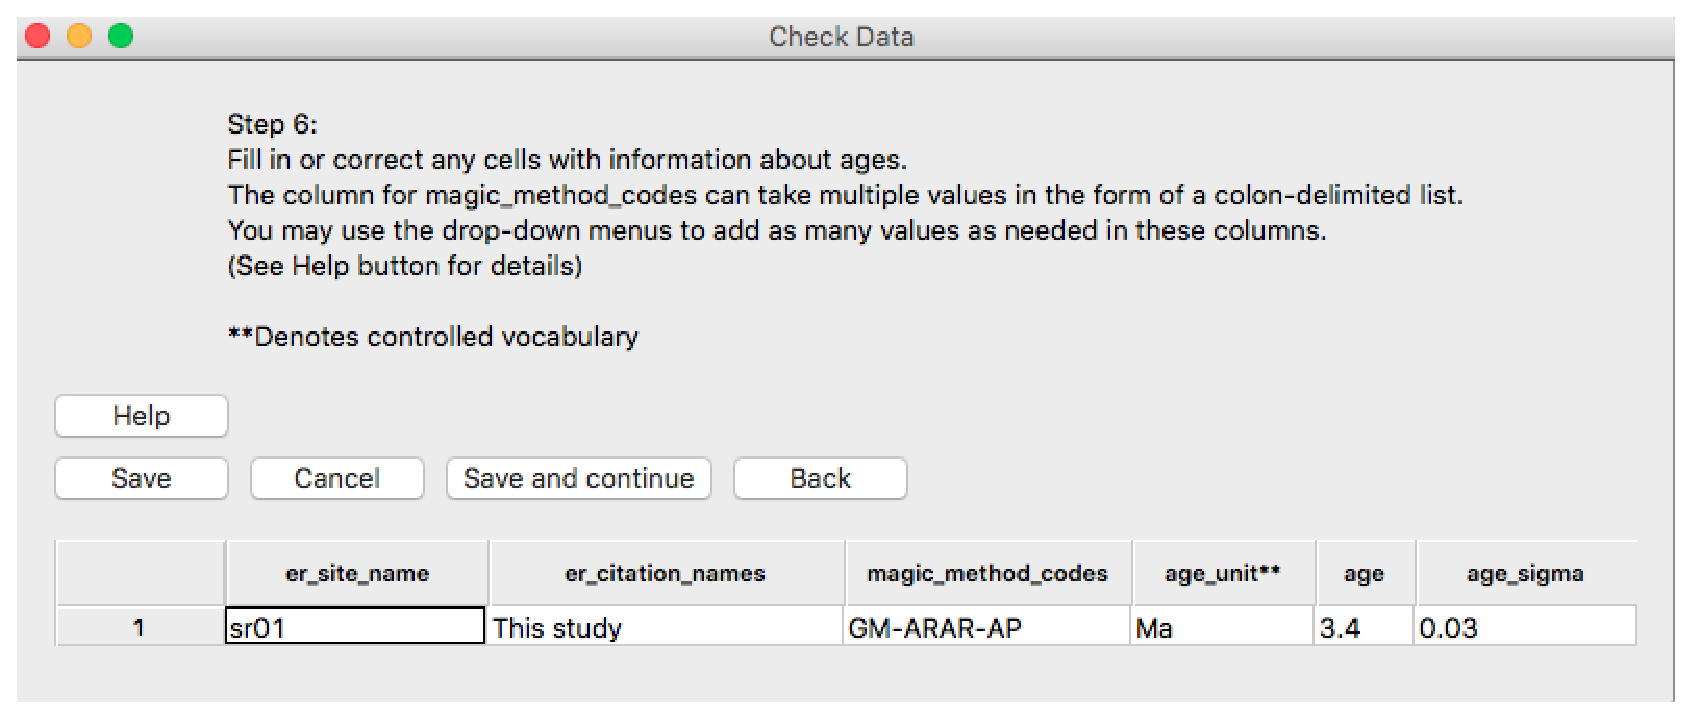
\includegraphics[width=32cm] {EPSfiles/FigErMagicStep6.eps}

\item Note that if you re-run this sequence, certain values may be changed or overwritten.  For example, if you set sample\_lithology to be something different from site\_lithology, re-running ErMagic will cause sample\_lithology to revert back to being the same as site\_lithology.
\item You are now ready to move on to making some interpretations!


\end{itemize}

\customlink{DemagGUI}

\section{Demag GUI program}
\label{sect:demag_gui}

This is the main panel of the demag GUI:

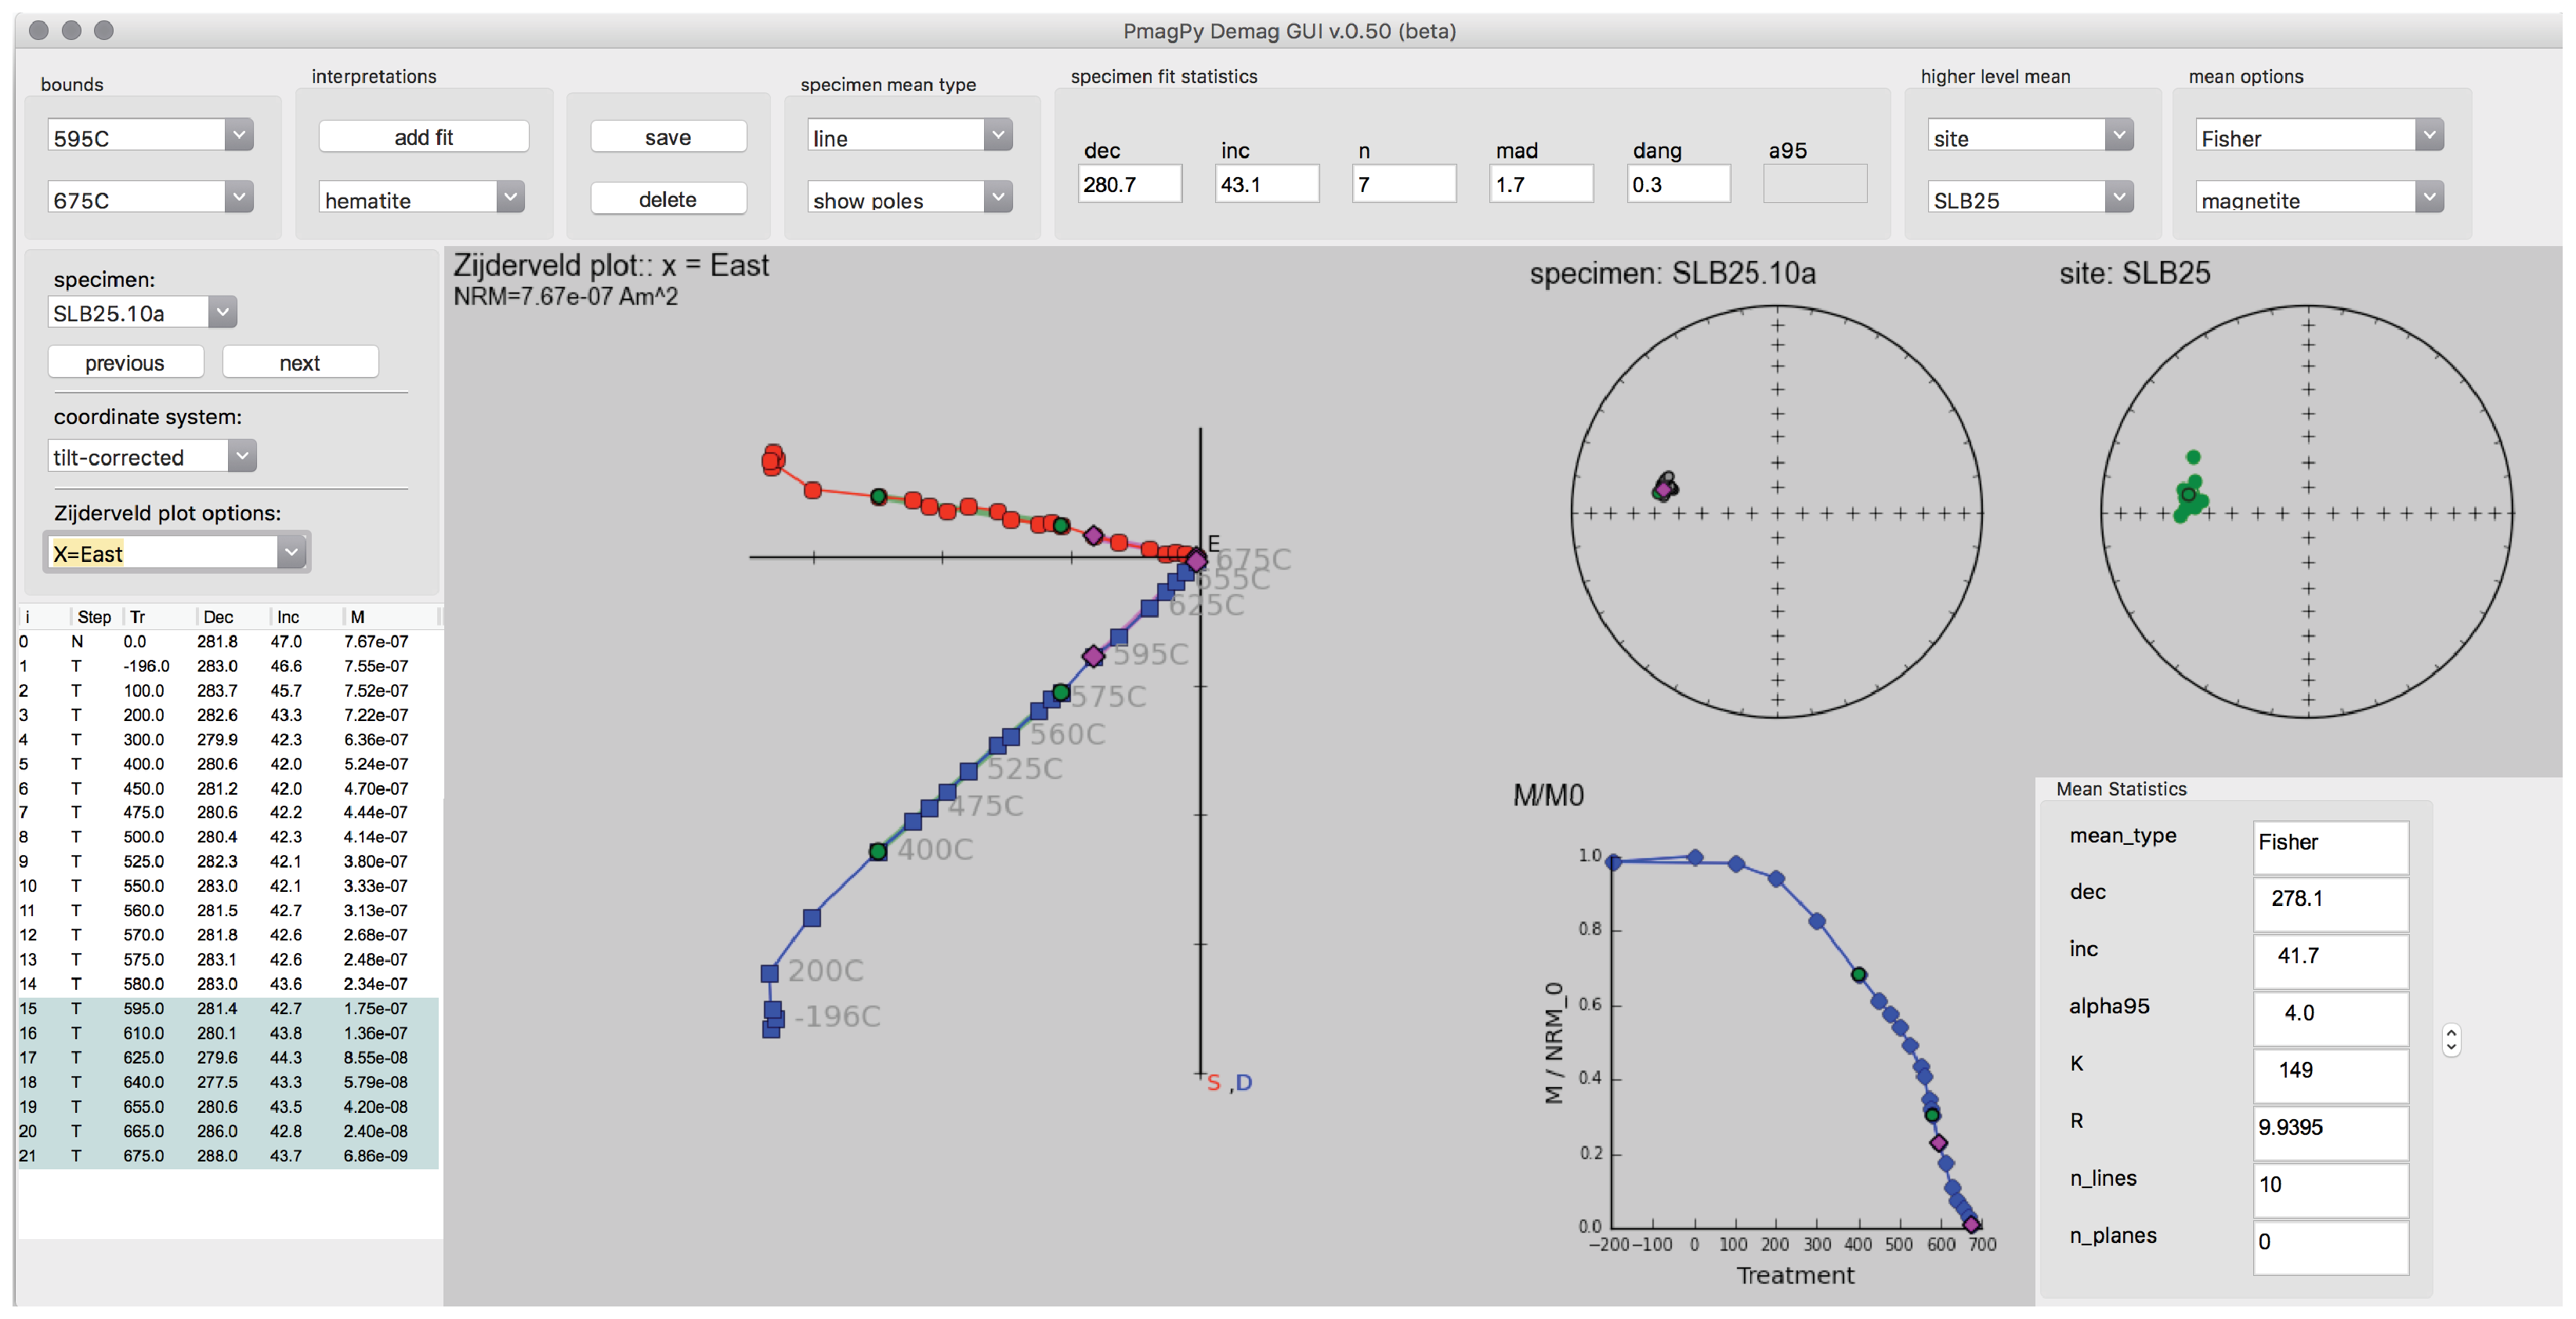
\includegraphics[width=30cm]{EPSfiles/demag_gui.eps}

To analyze the data in the example, follow these steps for each specimen:
\begin{itemize}
\item From the `coordinate system' drop down menu you can choose the coordinate system in which you wish to view the data (e.g.  `geographic').
\item Click `add a fit' and choose the temperature/AF bounds for the fit by double clicking on the measurement lines or by choosing from the `bounds' dropdown menu.
\item Click the `next' button to analyze the next specimen.
\item To calculate  Fisher mean for the site: choose from the `higher level mean' drop down menus: show=specimens; mean=Fisher.
\item All of the fits can be viewed and modified using the Interpretation Editor which can be selected from the Tools menu in the top menubar.
\item To save all of the specimen interpretations, choose from the menubar [File] $\rightarrow$ [Save MagIC pmag tables]. This saves all the interpretations in MagIC formatted pmag\_* files in your \href{#Project_Directory}{\it ThisProject} directory. Fits that are saved this way will be loaded into demag\_gui the next time it is launched.
\item Click through the dialog boxes and fill out choices for the MagIC results table.
\item Close the Demag GUI.
\end{itemize}

\section{Thellier GUI program}
This is main panel of \href{#thellier_gui}{Thellier GUI}:

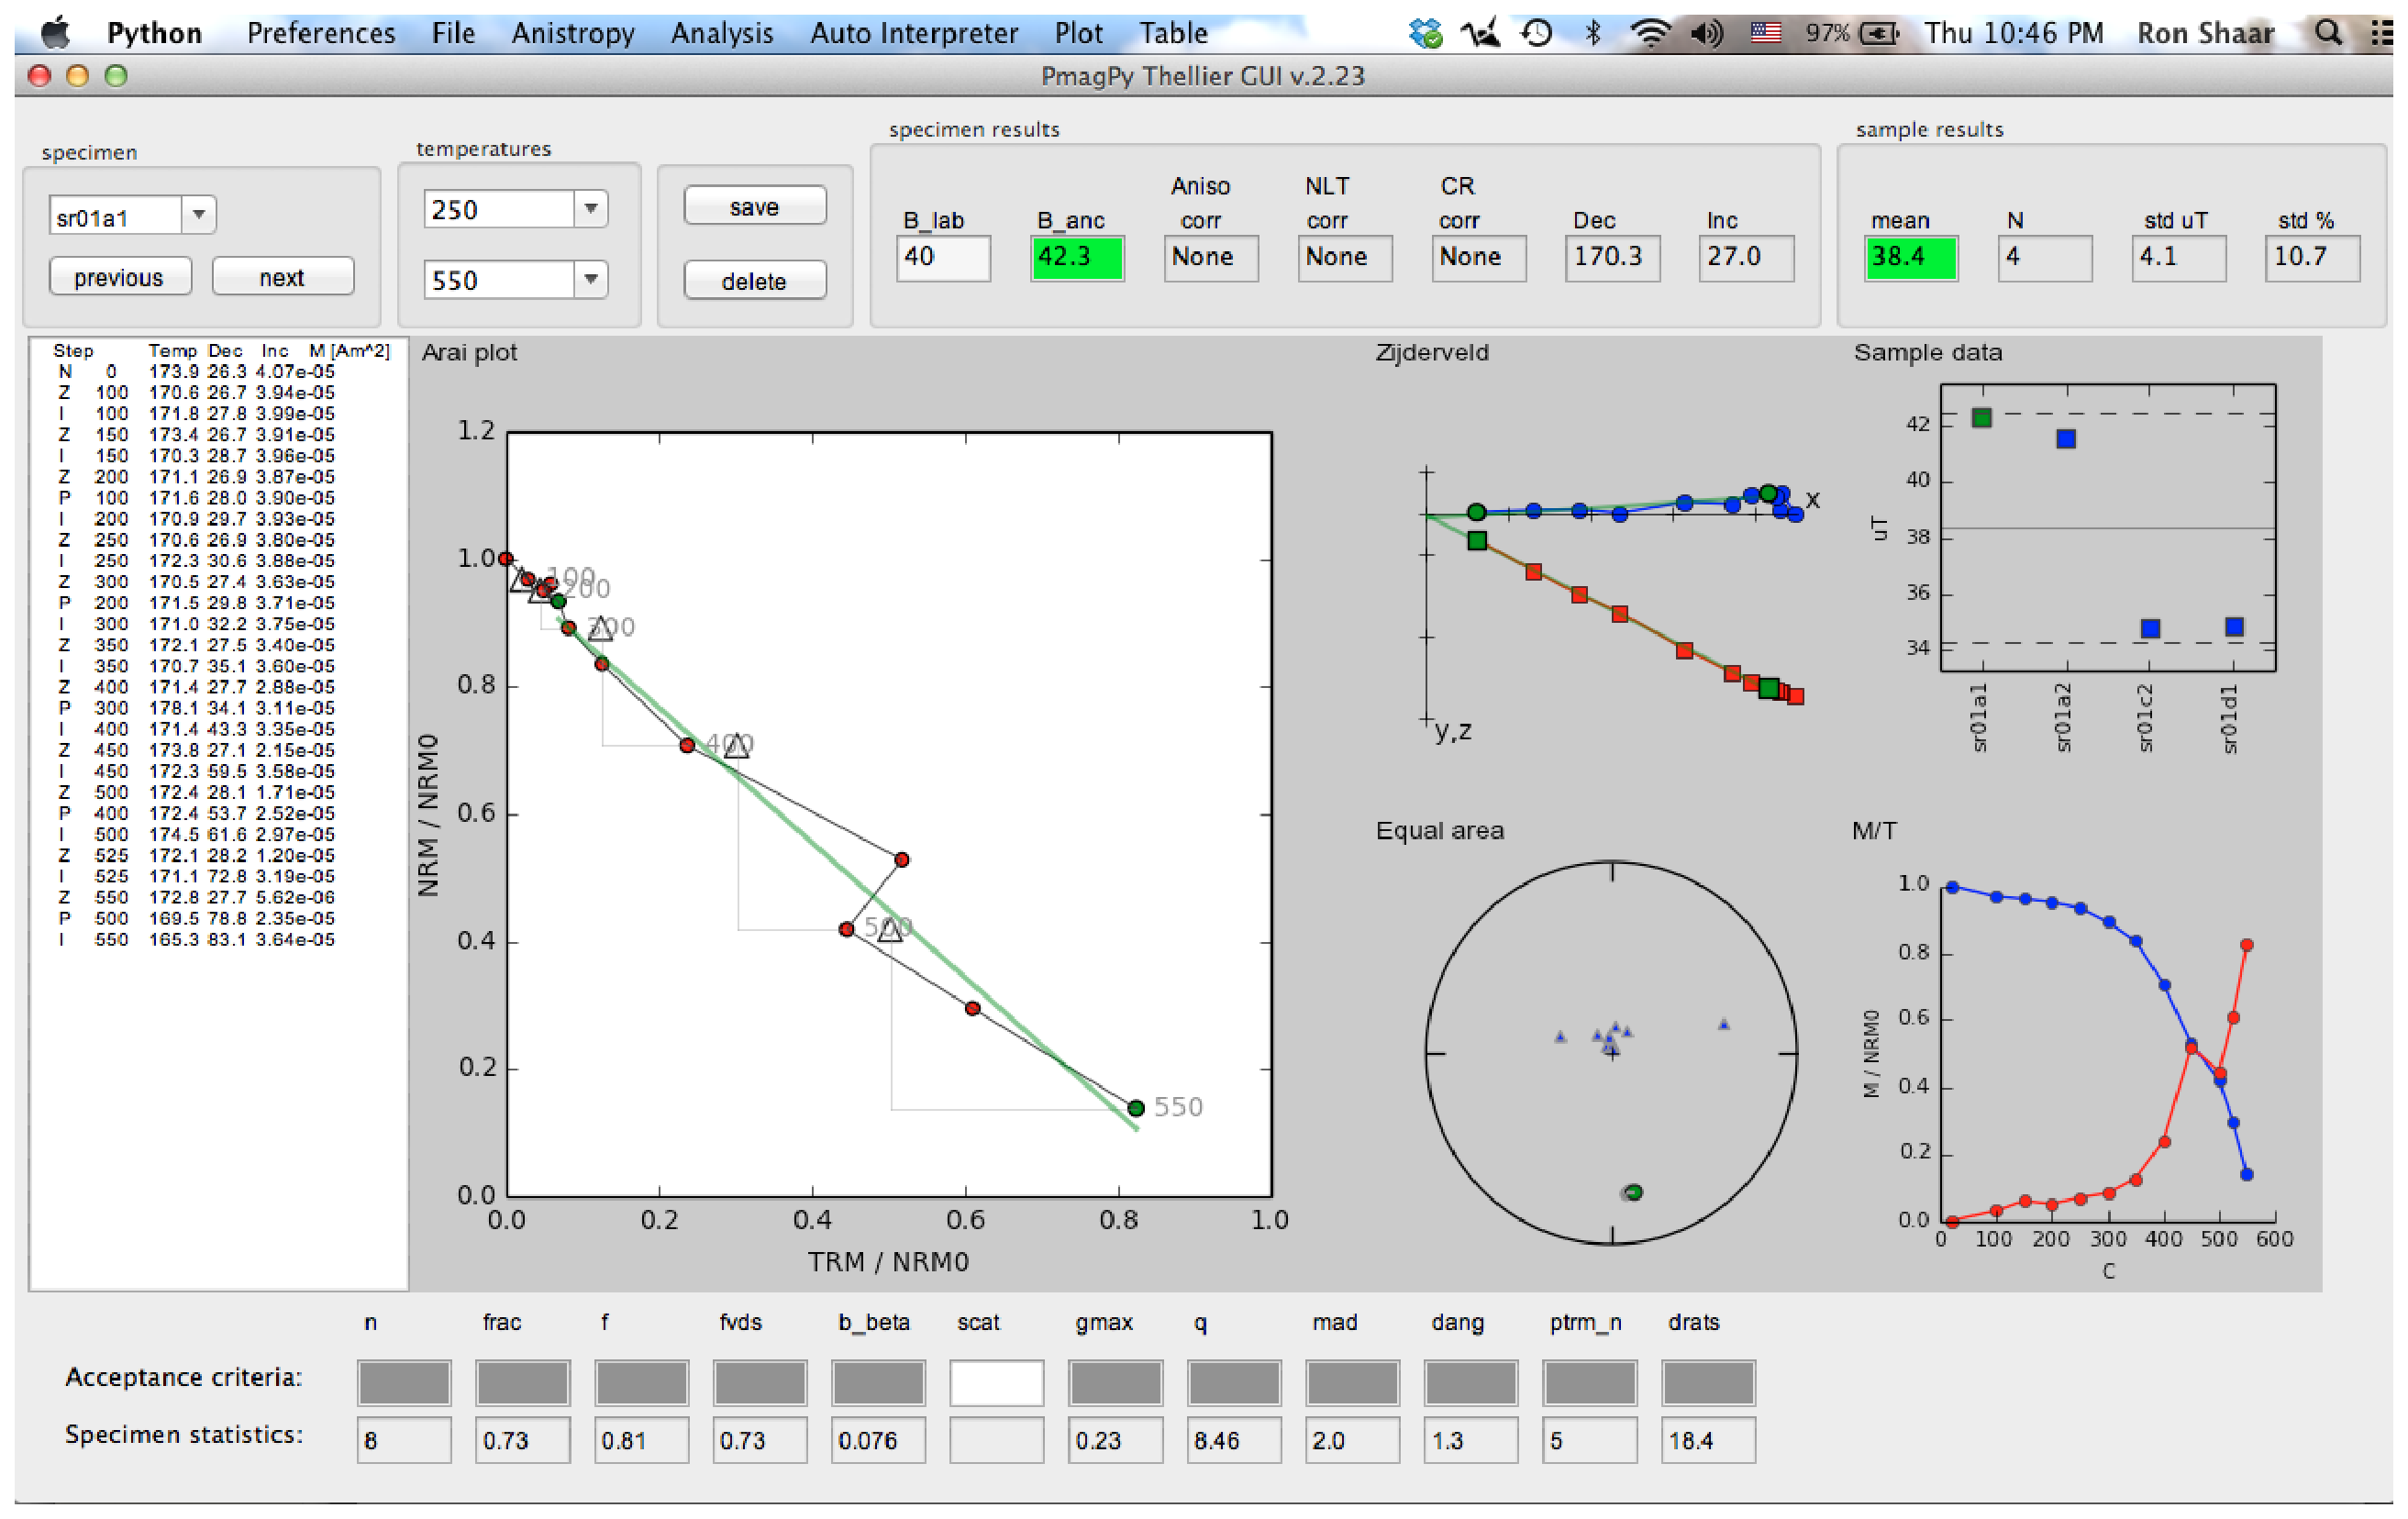
\includegraphics[width=30cm]{EPSfiles/FigThellierGui.eps}

 To analyze the data in the example, follow these steps for each specimen:
 \begin{itemize}
\item Choose temperature bounds from the temperatures dropdown menus.
\item  Click `save' so the program remembers the interpretations (the interpretation is not saved to a file yet!).
\item  Click the `next' button to analyze the next specimen.
\item The default of the program is to calculate sample means. To change it to site level mean, choose from the menubar: [Analysis $\rightarrow$ [Acceptance criteria] $\rightarrow$  [Change acceptance criteria]. Find the `average by sample/site' dropdown menu in the third row and change it to [site]. Click OK. The site mean will appear in the sample/site results box (top right).
\item  After all specimen interpretations are saved in memory, choose from the menubar [File] $\rightarrow$ [Save MagIC pmag tables]. This save all the interpretations in MagIC formatted pmag\_* files in the MagIC Project Directory.
\item  Close the Thellier GUI.
\end{itemize}

\customlink{magic_upload}

\section{Upload to the database }

For this, you first click on the green {\it prepare upload txt file} button on the main page of {\bf Pmag GUI}. A file named `upload.txt' will be created in your \href{#Project_Directory}{\it ThisProject} directory.  Now, go to the  \href{http://earthref.org/MAGIC/search}{MagIC search interface}.      Click on the `create' button and find or create your reference.

Click on `Upload' in the Actions column and   drag and drop the {\it upload.txt}   file onto the  `Drop a MagIC Text File' window.
Congratulations. Your data are now in the database.  But, they are not yet activated which you can do by clicking on the `Activate' button in the Actions column.  Once you activate an uploaded dataset (only for published papers), it will be publicly available.

\customlink{magic_download}

\section{Downloading data from {\bf MagIC}}

Data can be downloaded from the {\bf MagIC} database and examined with {\bf PmagPy} tools.   The \href{http://earthref.org/MAGIC/search/}{\bf MagIC} search interface provides a rich variety of search filters available by clicking on the `Filter the MagIC Search Results' text box.    To locate data from a particular reference,  simply substitute the digital object identifier (DOI) in your browser window:

\href{http://earthref.org/MAGIC/doi/10.1029/2003GC000661}{http://earthref.org/MAGIC/doi/10.1029/2003GC000661}

\noindent The above DOI will find the data for the paper by \cite{tauxe04b}.  [This may fail in Safari; if so, use an alternative browser like Firefox or Chrome.]     To download the data, simply click on the file icon below the column labeled `data'.  This will save a file to your downloads folder.
 To unpack this file after downloading it from the database click the ``unpack downloaded txt file button`` in the \href{#pmag_gui.py}{Pmag GUI}  panel.


 \section{Preparing for MagIC}

\customlink{field_info}

\subsection{Field and sampling information}

 There is an astounding number of different ways that paleomagnetists document data in the field and in the lab. This variety is met with a large number  of method codes that describe sampling and orientation procedures (see \url{http://earthref.org/MAGIC/methods.htm} for a complete description).   The MagIC database expects sample orientations to be the azimuth and plunge of the fiducial arrow used for measurement (see  \href{http://earthref.org/MAGIC/books/Tauxe/Essentials/WebBook3ch2.html#ch2}{[Essentials, Chapter 9]} )  and the orientation of the bedding to be dip direction and downward dip so no matter what your own preference is, it must be translated into the standard MagIC convention for use with the PmagPy programs and with \href{#pmag_gui.py}{Pmag GUI}.

\href{#pmag_gui.py}{Pmag GUI}  supports two different ways of getting orientation and other sampling related information into a MagIC usable format.  The first way is through \href{#orient}{step 2 on the GUI front panel} and filling in the data from within the GUI.  That way will work for many applications, but it may be desirable to fill the spreadsheet in separately from the GUI by using  a tab delimited file (orient.txt format).   By clicking on  \href{#orient}{step 2 on the GUI front panel}  you create a file named {\it demag\_orient.txt}  which has all of your sample names in it.   Each {\it orient.txt} file should  have all the information for a single location {\it sensu MagIC}.


  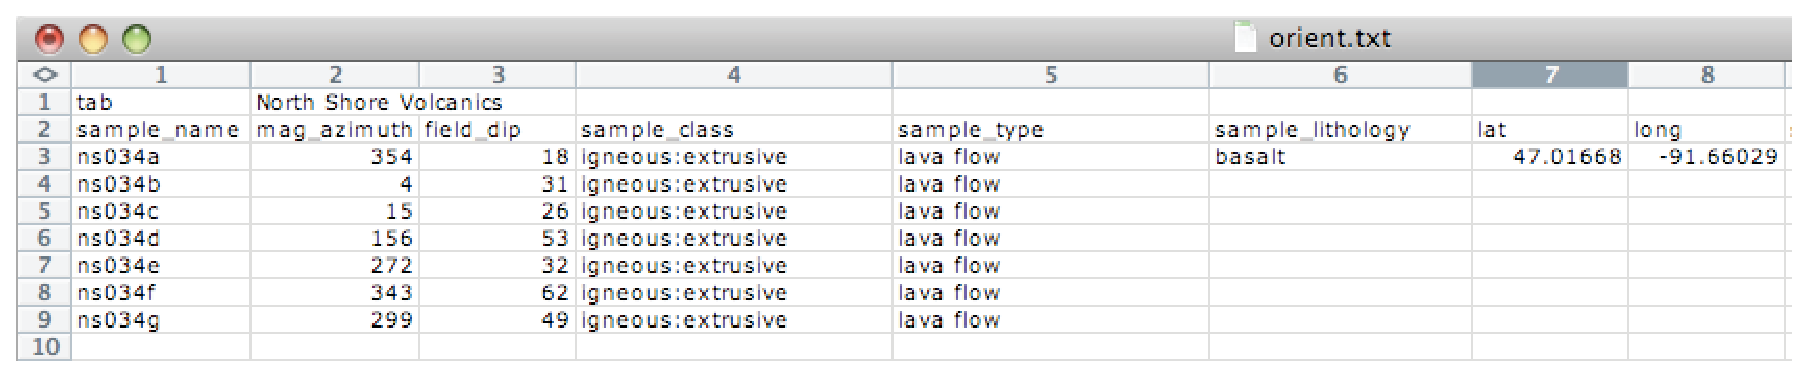
\includegraphics[width=15cm]{EPSfiles/orient.eps}

 The next row has the names of the columns.  The required columns are:  sample\_name, mag\_azimuth, field\_dip, date, lat, long, sample\_lithology, sample\_type, sample\_class) but there are a number of other possible columns (e.g., Optional Fields in orient.txt formatted files are: [date, shadow\_angle, hhmm], date, stratigraphic\_height, [bedding\_dip\_direction, bedding\_dip], [image\_name, image\_look, image\_photographer], participants, method\_codes, site\_name, and site\_description, GPS\_Az]).  Column names in brackets must be supplied together and the data for stratigraphic\_height are in meters.  Also note that if these are unoriented samples, just set mag\_azimuth and field\_dip to 0.

% If there is a simple  and consistent relationship between the site name and the sample name (e.g., sample ns034a belongs to site ns034), you do not need to specify a site name here as it will be parsed by \href{#orientation_magic.py}{orientation\_magic.py} when it gets converted  to the MagIC format.  However, many investigators have no such consistent naming scheme.  Moreover, in some cases,  groups of samples or initial site designations need to be re-grouped for averaging.  For example, if it becomes clear that a sequence of lava flows were erupted over a short period of time and should be averaged together, you would need a new site name for all the samples.  Note that there are different understandings of the term {\bf site} in the paleomagnetic community.  We adhere to the MagIC definition of ``site'', which is:
% \begin{quote}
%site: a group of samples that are homogeneous with respect to the property being measured.
%\end{quote}
%\noindent When a site  has no simple relationship to the sample names, a column named  site\_name in the {\it orient.txt} file can be used  with the site name filled in for every sample.

   It is handy  to document the lithology, type and material classification information required by MagIC. These  are all controlled vocabularies listed at \url{http://earthref.org/MAGIC/shortlists.htm}.   For archaeological materials, set the lithology to ``Not Specified''.

   Put in stratigraphic height, sun compass, differential GPS orientation information under the appropriate column headings.  You can also flag a particular sample orientation as suspect, by having a column 'sample\_flag' and setting it to either 'g' for good or 'b' for bad.  Other options include documenting digital field photograph names and who was involved with the sampling.

 For Sun Compass measurements, supply the shadow\_angle, date and time. The date must be in mm/dd/yy format. If you enter the time in local time, be sure you know the offset to Universal Time as you will have to supply that when you import the file. Also, only put data from one time zone in a single file. The shadow angle should follow the convention shown in this figure (from Tauxe et al., 2010): \nocite{tauxe10}

  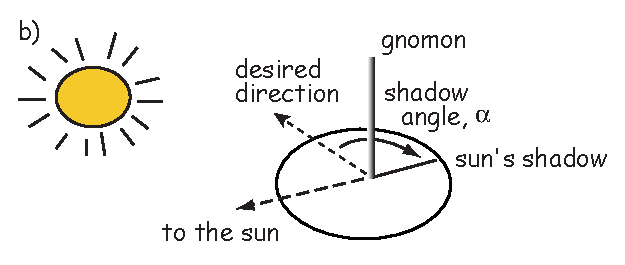
\includegraphics[width=15cm]{EPSfiles/suncomp.eps}

  \customlink{orientation_schemes}

{\bf Supported sample orientation schemes:}

  There are options for
 different orientation conventions (drill direction with the Pomeroy orientation device  [drill azimuth and hade] is the default), different naming conventions and a choice of whether to automatically calculate the IGRF value for magnetic declination correction, supply your own or ignore the correction.  The program generates {\it er\_samples.txt} and {er\_sites.txt} files.  Be warned that existing files with these names will be overwritten.

 All images, for example outcrop photos are supplied as a separate zip file. image\_name is the name of the picture you will import, image\_look is the ``look direction`` and image\_photographer is the person who took the picture. This information will be put in a file named er\_images.txt and will ultimately be read into the er\_image table in the console where additional information must be entered (keywords, etc.).

Often, paleomagnetists note when a sample orientation is suspect in the field. To indicate that a particular sample may have an uncertainty in its orientation that is greater than about 5$^{\circ}$, enter SO-GT5 in the method\_codes column and any other special codes pertaining to a particular sample from the method codes table. Other general method codes can be entered later. Note that unlike date and sample\_class, the method codes entered in orient.txt pertain only to the sample on the same line.

Samples are oriented in the field with a ``field arrow`` and measured in the laboratory with a ``lab arrow``. The lab arrow is the positive X direction of the right handed coordinate system of the specimen measurements. The lab and field arrows may not be the same. In the MagIC database, we require the orientation (azimuth and plunge) of the X direction of the measurements (lab arrow). Here are some popular conventions that convert the field arrow azimuth (mag\_azimuth in the orient.txt file) and dip (field\_dip in orient.txt) to the azimuth and plunge of the laboratory arrow (sample\_azimuth and sample\_dip in er\_samples.txt). The two angles, mag\_azimuth and field\_dip are explained below.

{\parindent 0pt
[1] Standard Pomeroy convention of azimuth and hade (degrees from vertical down) of the drill direction (field arrow). sample\_azimuth = mag\_azimuth; sample\_dip =-field\_dip.

  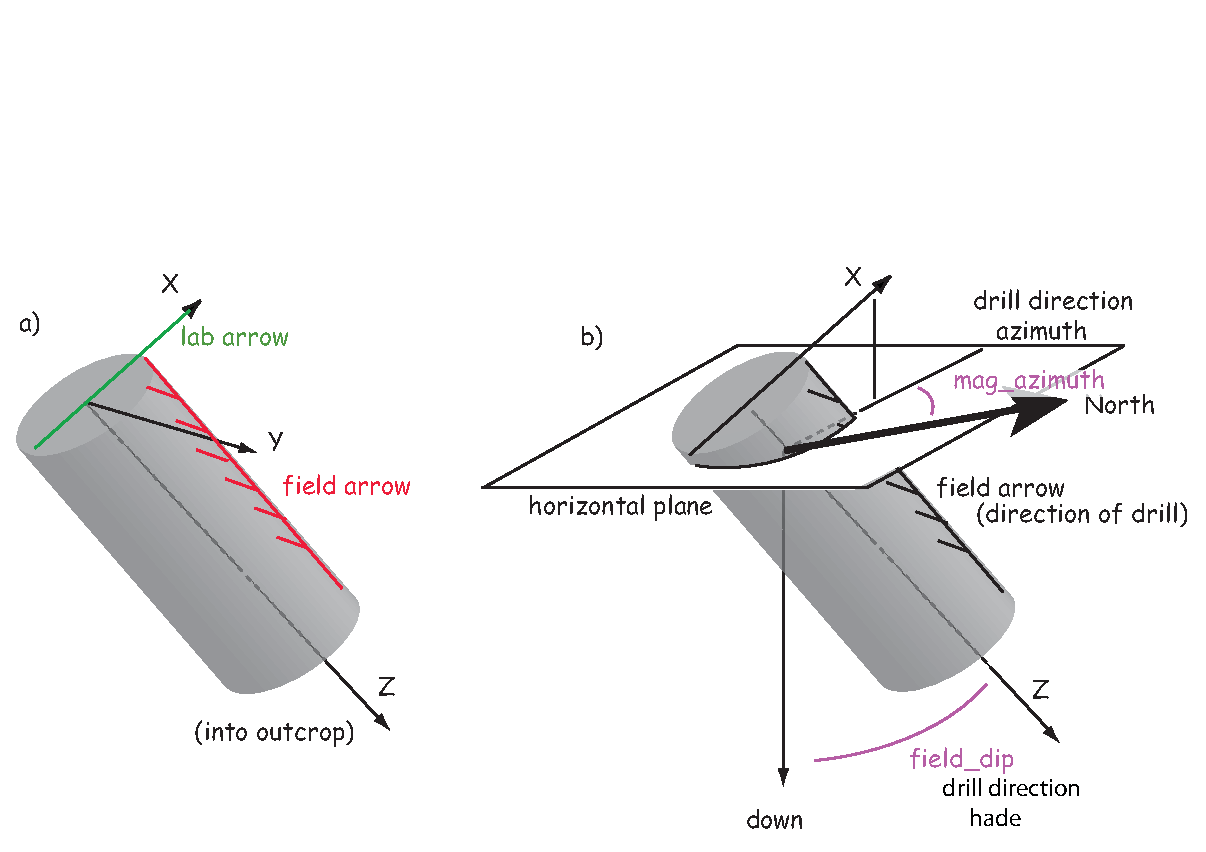
\includegraphics[width=15cm]{EPSfiles/orcon_1.eps}

  2] Field arrow is the strike of the plane orthogonal to the drill direction, Field dip is the hade of the drill direction. Lab arrow azimuth = mag\_azimuth-90$^{\circ}$; Lab arrow dip = -field\_dip

    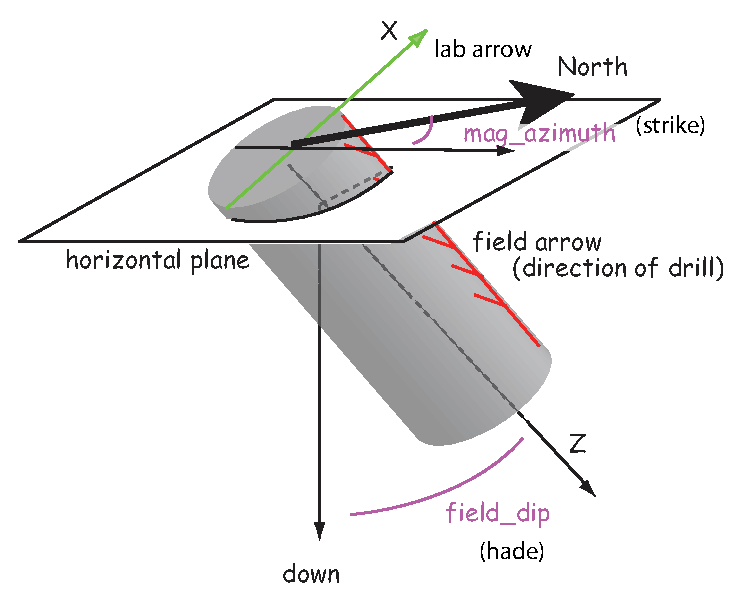
\includegraphics[width=15cm]{EPSfiles/orcon_2.eps}

  [3] Lab arrow is the same as the drill direction; hade was measured in the field. Lab arrow azimuth = mag\_azimuth; Lab arrow dip = 90$^{\circ}$-field\_dip.

      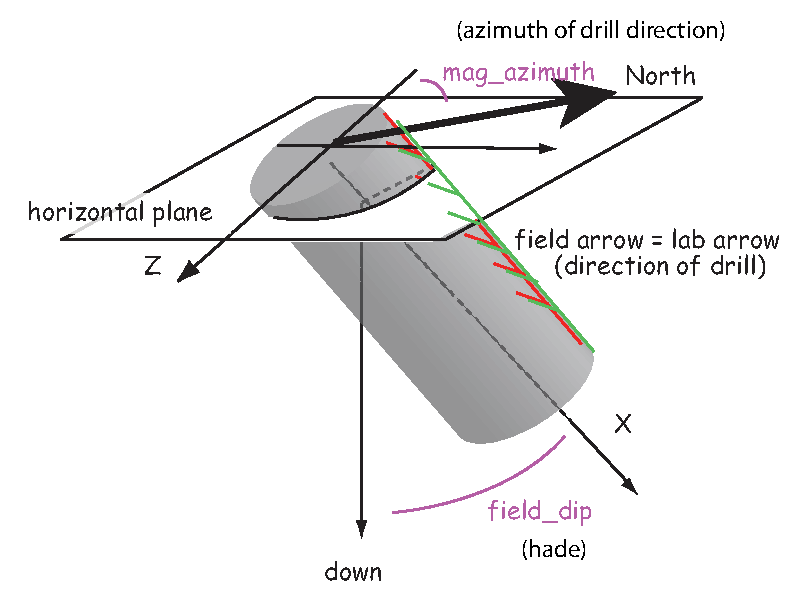
\includegraphics[width=15cm]{EPSfiles/orcon_3.eps}

  [4] Lab arrow orientation same as mag\_azimuth and field\_dip.

        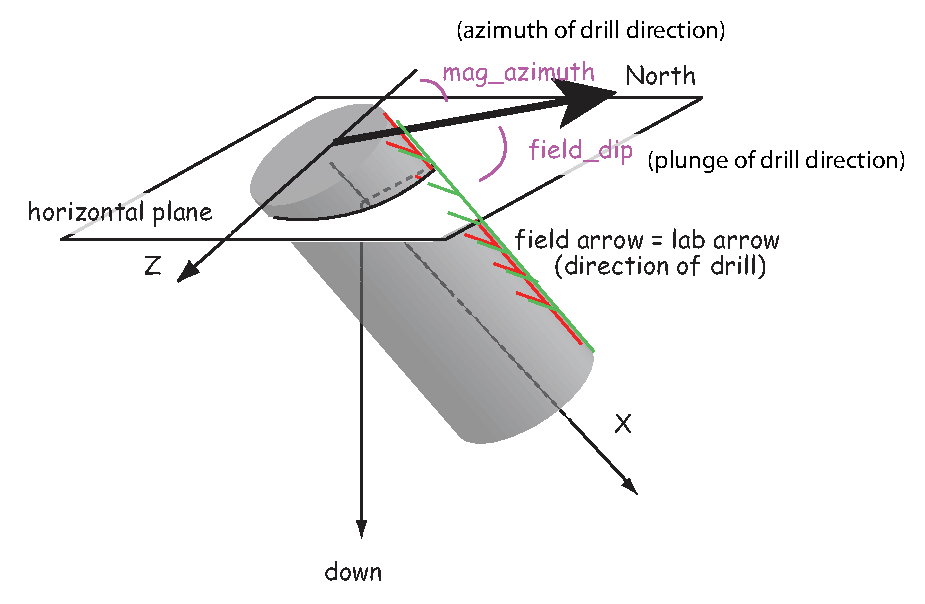
\includegraphics[width=15cm]{EPSfiles/orcon_4.eps}

        [5]  Lab arrow azimuth is  mag\_azimuth and lab arrow dip is the  field\_dip-90$^{\circ}$

               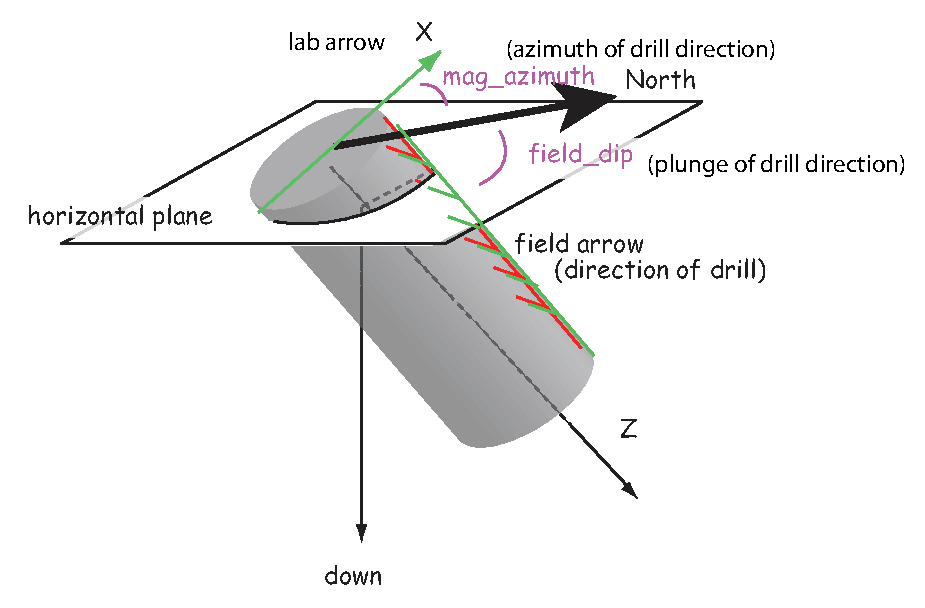
\includegraphics[width=15cm]{EPSfiles/orcon_5.eps}


 [6] Lab arrow azimuth is mag\_azimuth-90$^{\circ}$, Lab arrow dip is 90$^{\circ}$-field\_dip, i.e., the field arrow was strike and dip of orthogonal face:

                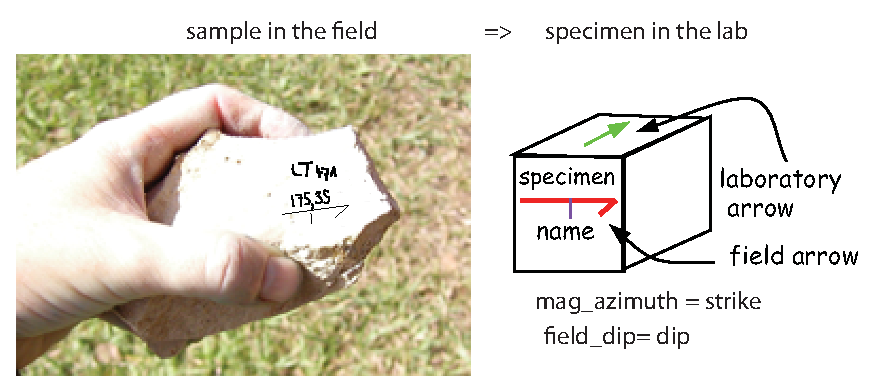
\includegraphics[width=15cm]{EPSfiles/orcon_6.eps}
                }

{\bf Structural correction conventions:}


Because of the ambiguity of strike and dip, the MagIC database uses the dip direction and dip where dip is positive from 0 $\rightarrow$ 180. Dips$ > $90 are overturned beds.


 \customlink{naming_schemes}

{\bf Supported sample naming schemes:}

\begin{verbatim}
            [1] XXXXY: where XXXX is an arbitrary length site designation and Y
                is the single character sample designation.  e.g., TG001a is the
                first sample from site TG001.    [default]
            [2] XXXX-YY: YY sample from site XXXX (XXX, YY of arbitary length)
            [3] XXXX.YY: YY sample from site XXXX (XXX, YY of arbitary length)
            [4-Z] XXXX[YYY]:  YYY is sample designation with Z characters from site XXX
            [5] site name = sample name
            [6] site name entered in site_name column in the orient.txt format input file
            [7-Z] [XXX]YYY:  XXX is site designation with Z characters from samples  XXXYYY
\end{verbatim}

When you are finished with editing the {\it orient.txt} file,  return to  \href{#orient}{step 2 on the GUI front panel}.


%
%\customlink{AZDIP}
%
%\subsubsection{AZDIP formatted files}
%
%This is a very simple file format with the sample name Azimuth Plunge Strike Dip where the Azimuth and Plunge are of the drill direction (Specimen's Z direction) or orientation convention \#3 above to convert to the MagIC standard. To convert strike to bedding dip direction, we would just add 90$^{\circ}$. Here is an example AzDip file:
%
%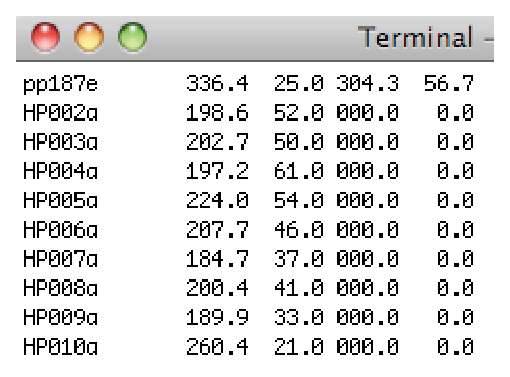
\includegraphics[width=15cm]{EPSfiles/azdip.eps}

\customlink{LIMS}

\subsubsection{Data files downloaded from the IODP (LIMS) database}


There are two types of files that help in plotting of IODP paleomagnetic data sets: the core summaries with depth to core top information and the sample information that contains lists of samples taken.
Visiting the IODP science query website at \url{http://web.iodp.tamu.edu/WTR/html/sci-data.html} allows you to
select 'SRM - Remanence of magnetization' under the Analysis scroll down menu.  By picking the expedition, site, hole, etc. you can download a  .csv format (comma separated values) for the expedition data.  (Be aware that this is the rawest form of the data, including disturbed intervals, bad measurements, core ends, etc. and may not be exactly what ended up getting published!).   First click on the ``Show Report`` button, then, ``Expand Table'', then ``Get File'':

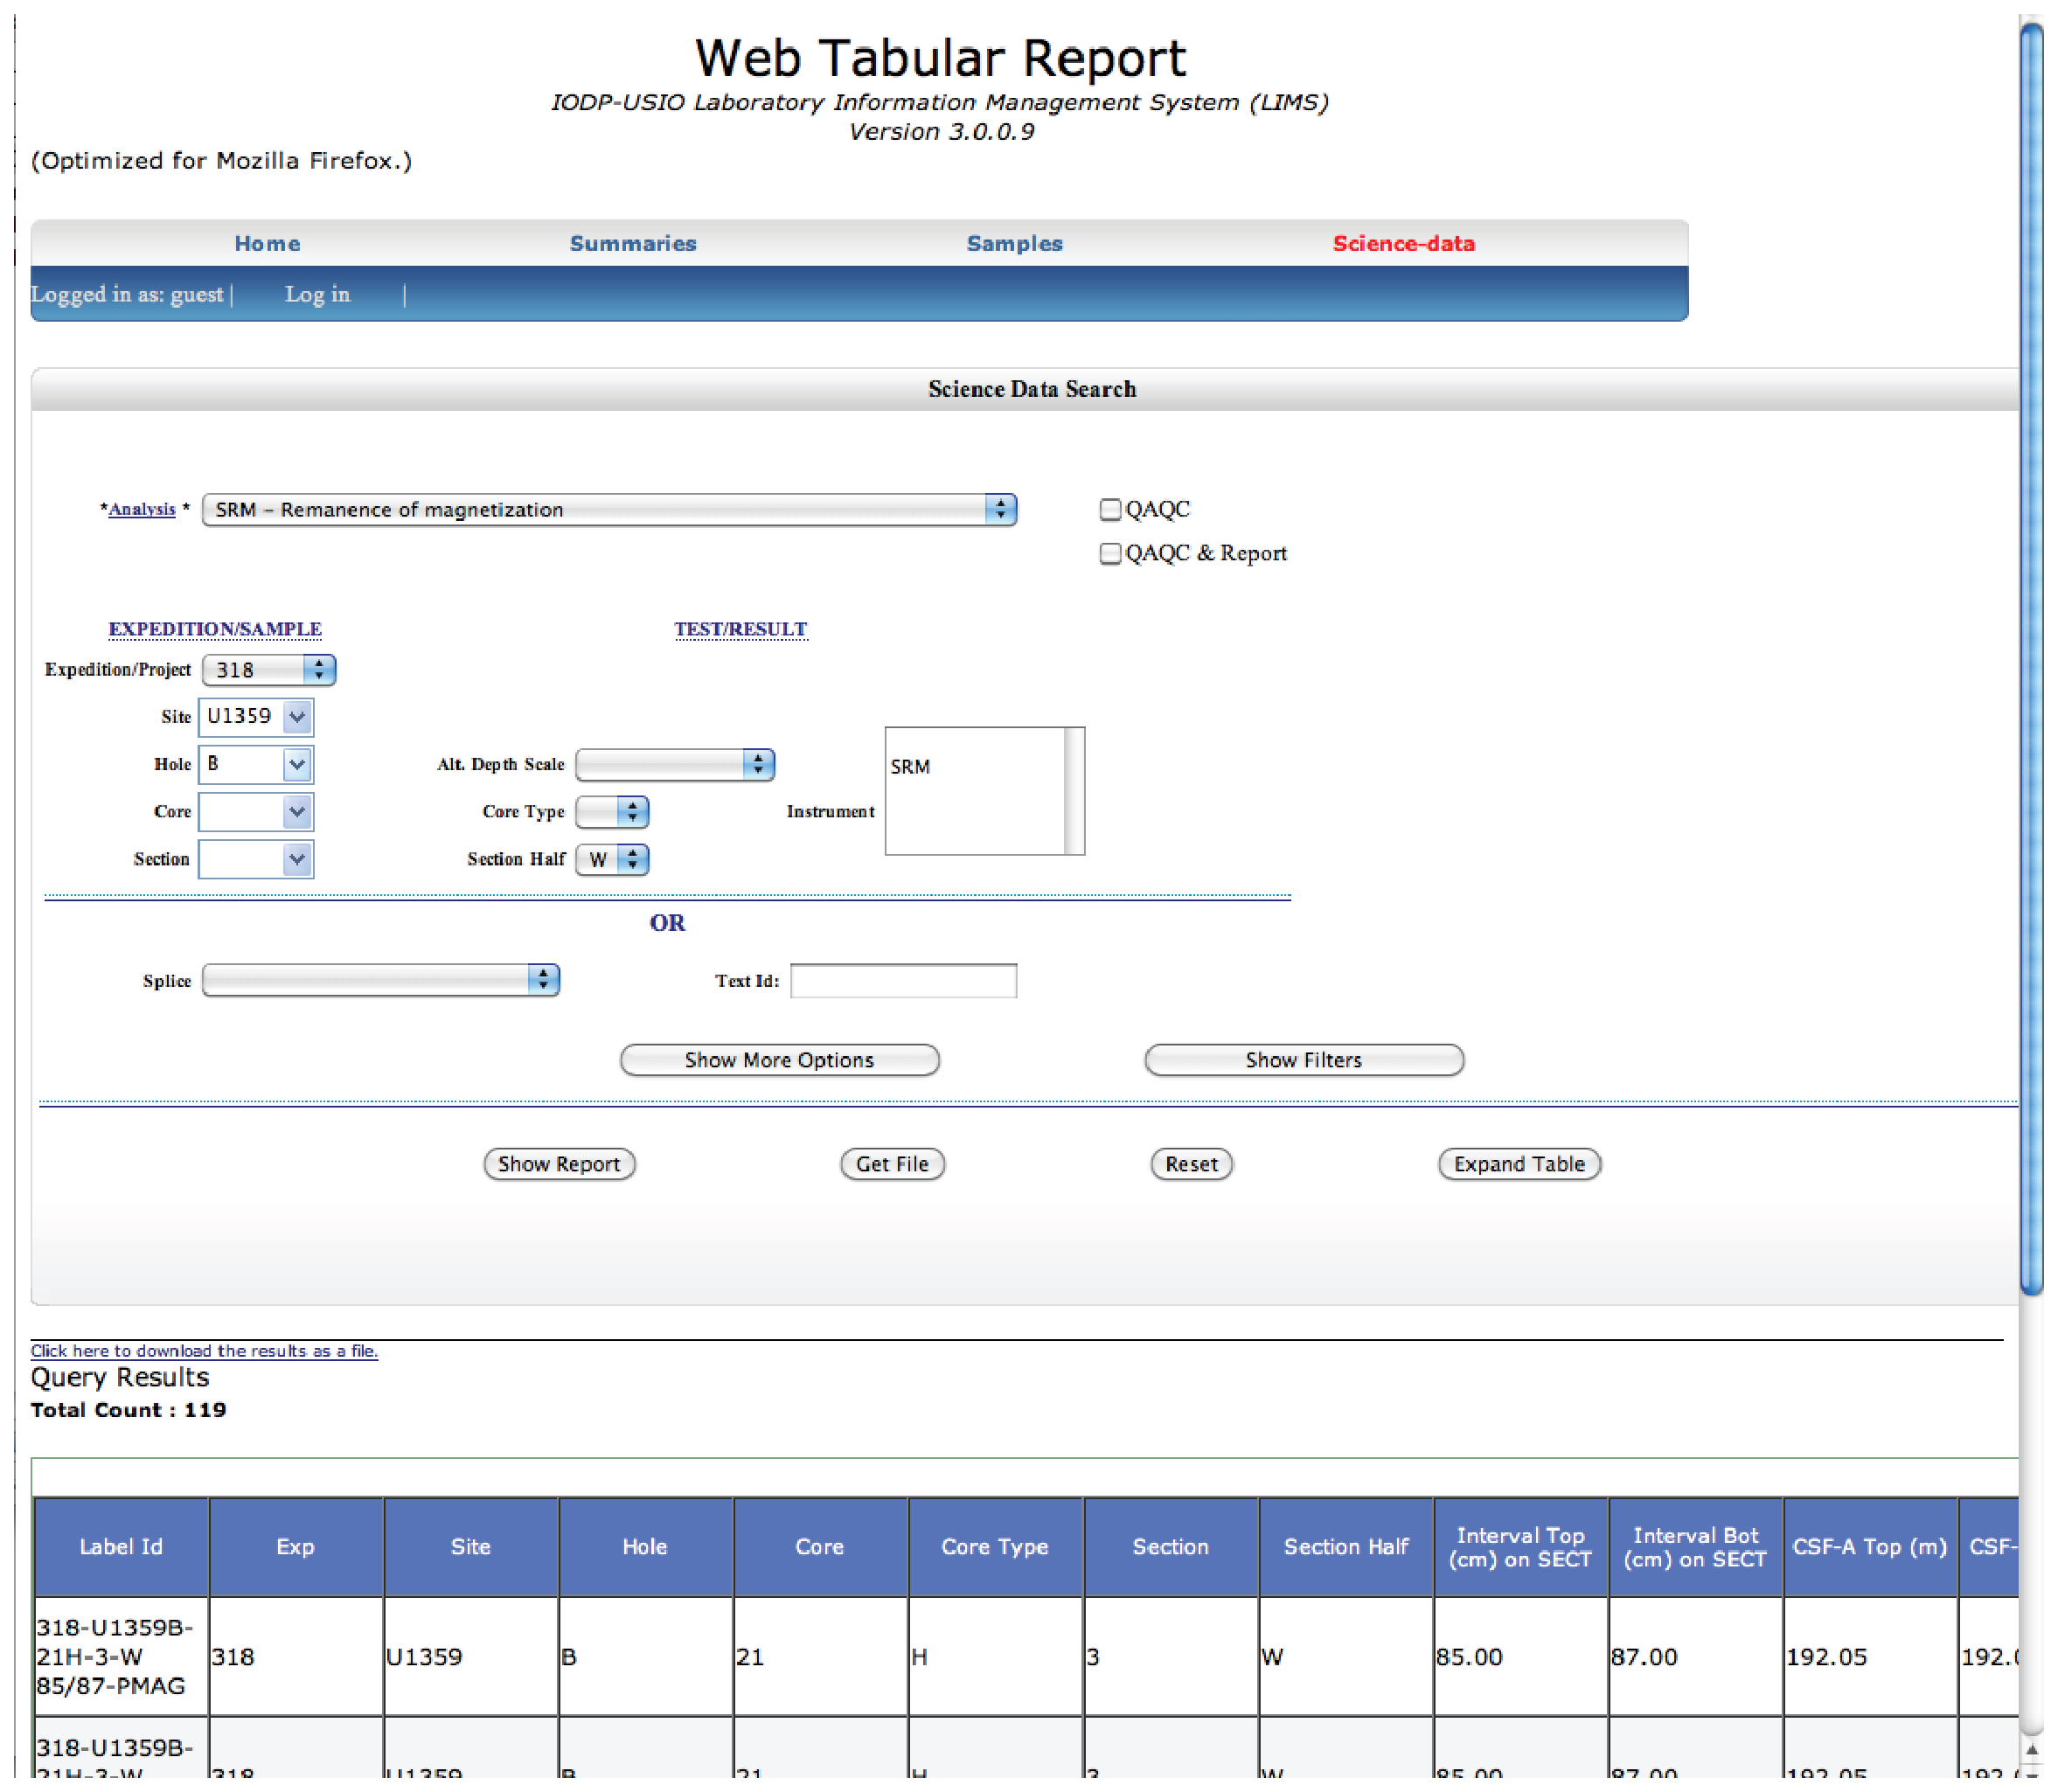
\includegraphics[width=15cm]{EPSfiles/WebTabular_srm.eps}

This can take a very long time, so get yourself a cup of tea.

You can also (while you're at it) click on the 'Summaries' tab and download the coring summaries:

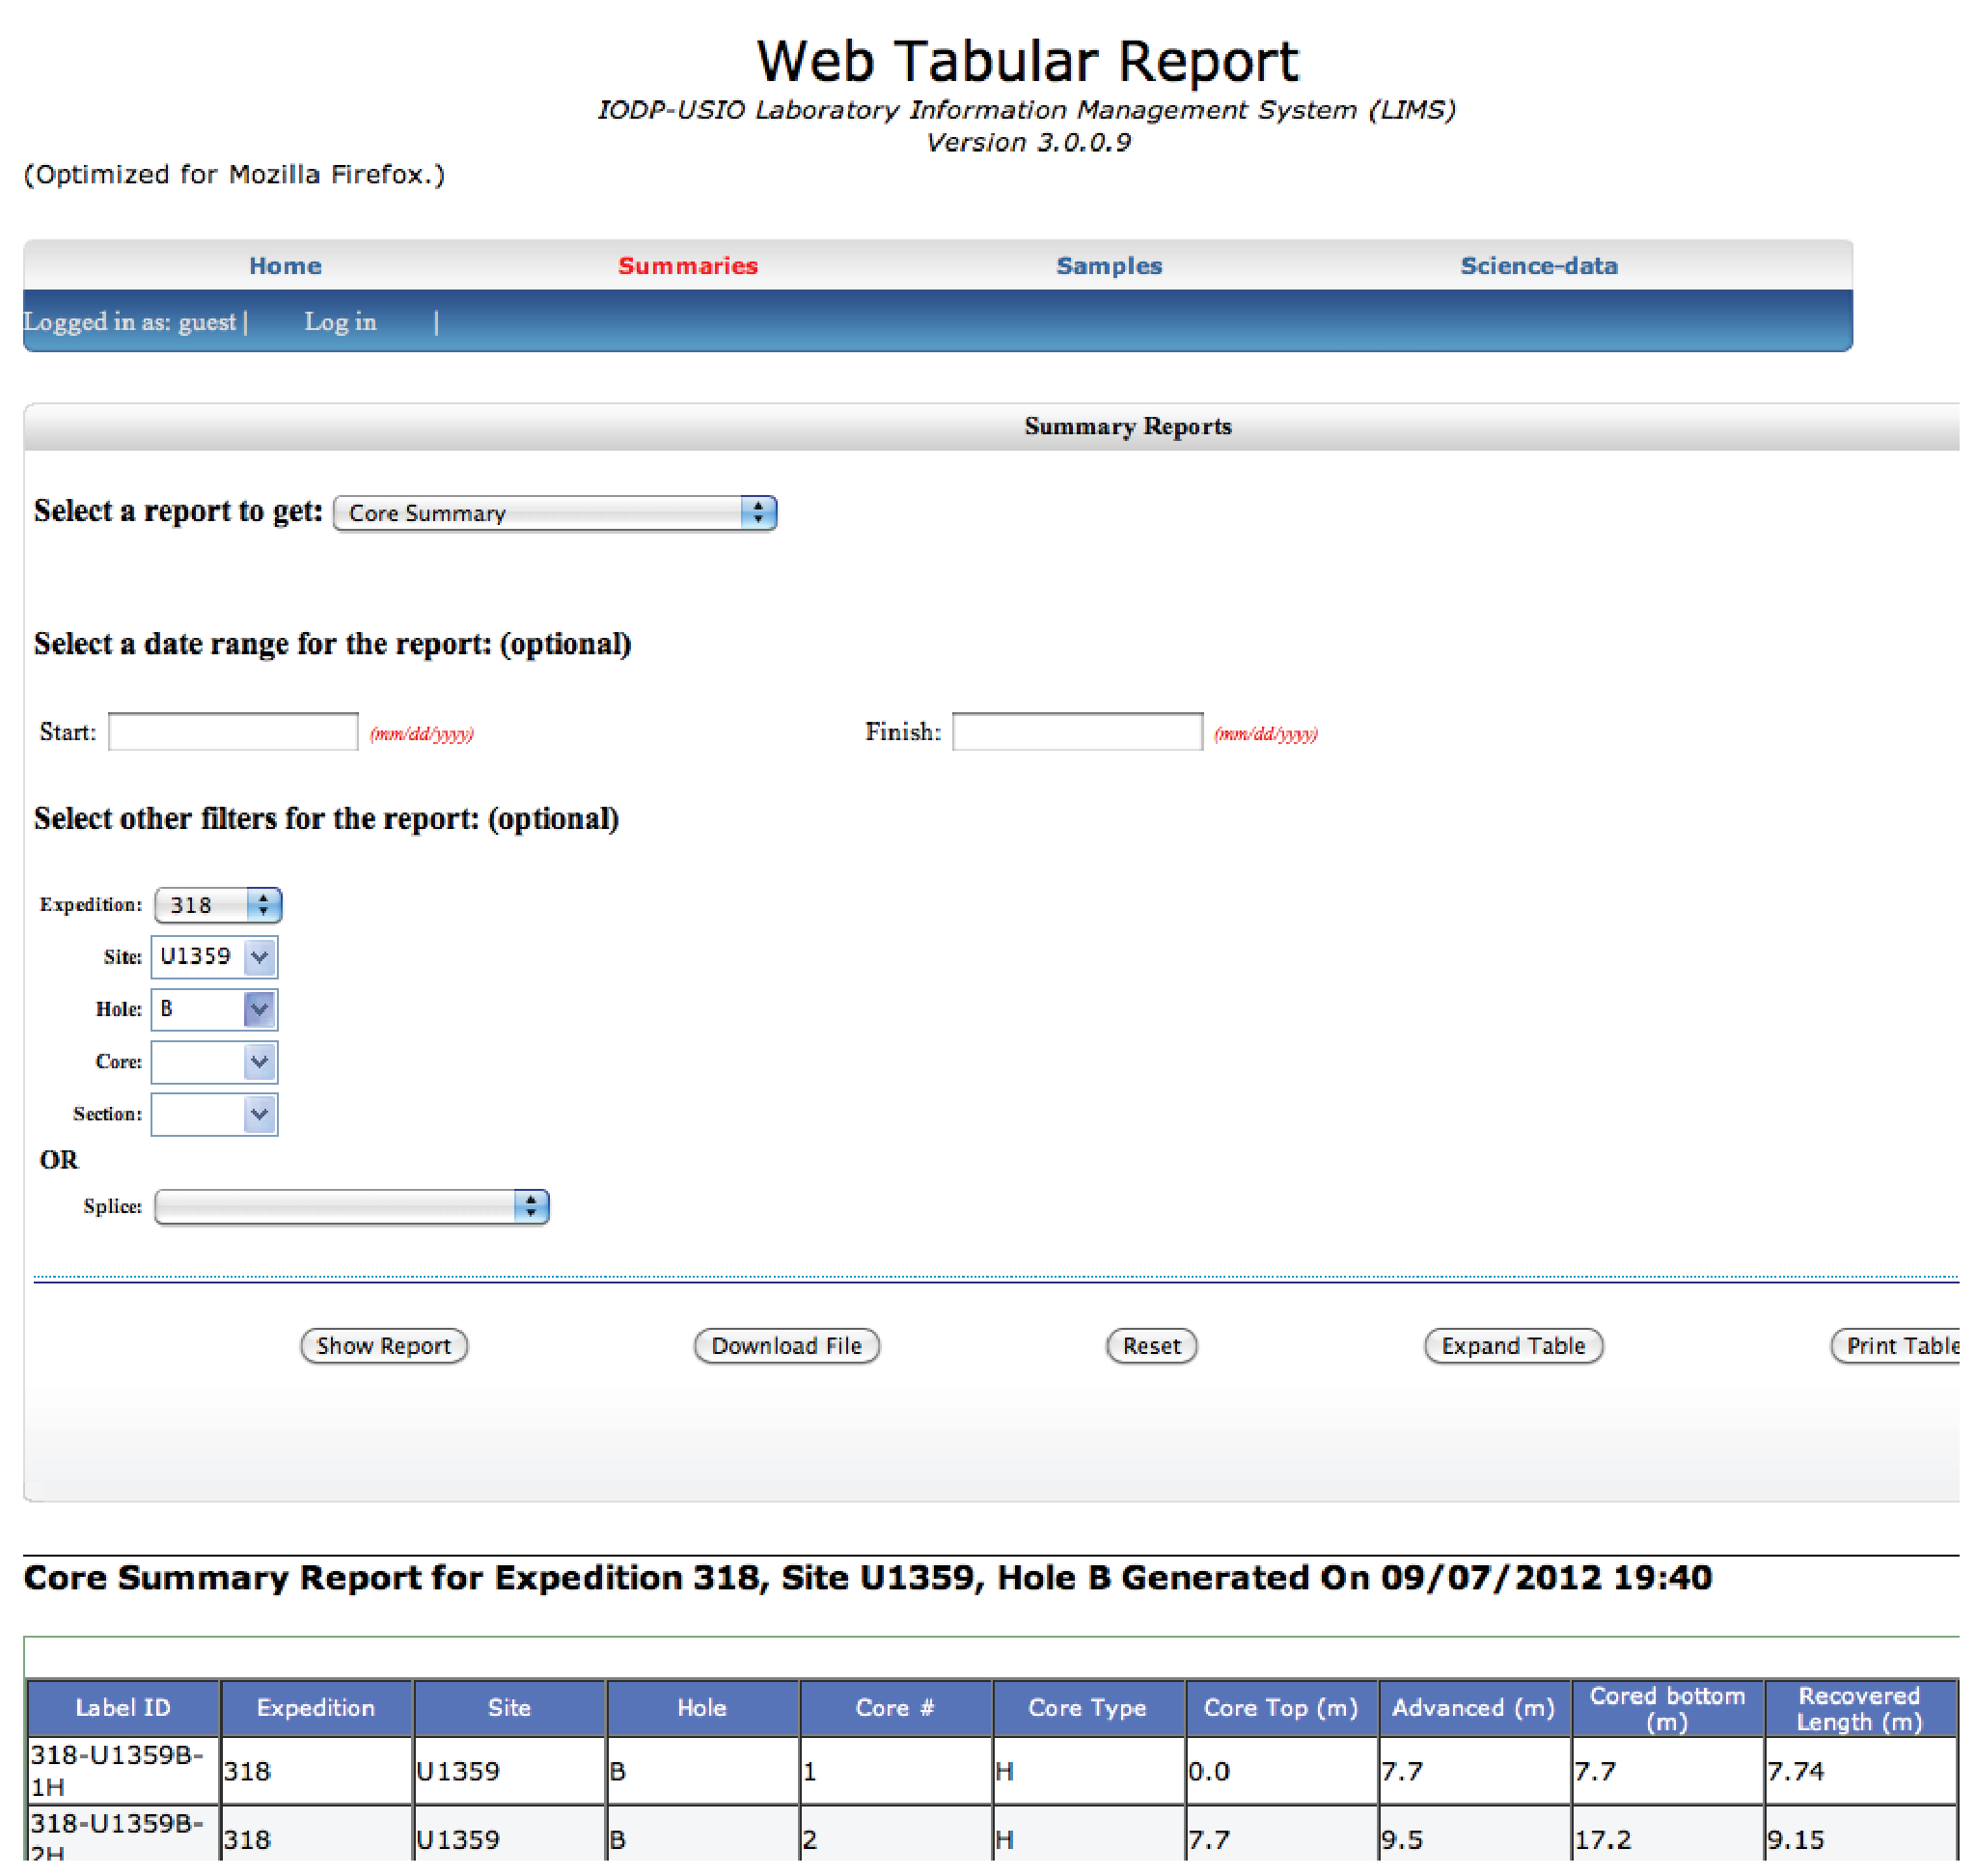
\includegraphics[width=15cm]{EPSfiles/WebTabular_core.eps}

Place both of the downloaded files in your {\it MyFiles} directory.


\customlink{magnetometer_files}

\subsection{Supported Rock Magnetometer files}

The MagIC database is designed to accept data from a wide variety of paleomagnetic and rock magnetic experiments. Because of this the magic\_measurements table is complicated. Each measurement only makes sense in the context of what happened to the specimen before measurement and under what conditions the measurement was made (temperature, frequency, applied field, specimen orientation, etc). Also, there are many different kinds of instruments in common use, including rock magnetometers, susceptibility meters, Curie balances, vibrating sample and alternating gradient force magnetometers, and so on. We have made an effort to write translation programs for the most popular instrument and file formats and continue to add new supported formats as the opportunity arises. Here we describe the various supported data types and tell you how to prepare your files for importing. In general, all files for importing should be placed in the MyFiles directory or in subdirectories therein as needed.  If you don't see your data type in this list, please send an example file and a request to:  ltauxe@ucsd.edu and we'll get it in there for you.


The supported file formats are:

{\bf Rock Magnetometer Files:}

\begin{itemize}
%\item \href{#2G_magic.py}{2G binary format}
\item \href{#CIT_magic.py}{The CalTech format used by labs in the RAPID consortium}
%\item \href{#FIN_magic.py}{whatever}
%\item \href{#FLA_magic.py}{Univ. Florida, Gainesville format}
\item \href{#HUJI_magic.py}{Hebrew University, Jerusalem format}
\item \href{#sio_magic.py}{Scripps Institution of Oceanography format}
\item \href{#LDEO_magic.py}{Lamont Doherty Earth Observatory format}
%\item \href{#LIVMW_magic.py}{Unviersity of Liverpool, microwave format}
\item \href{#IODP_csv_magic.py}{IODP rock magnetometer (SRM) data downloaded from the LIMS database}
\item \href{#PMD_magic.py}{PMD (ascii) format}
\item \href{#TDT_magic.py}{ThellierTool format}
%\item \href{#UB_magic.py}{University of Barcelona format}
%\item \href{#UCSC}{various UC Santa Cruz formats}
%\item \href{#UMICH_magic.py}{University of Michigan format}
%\item \href{#JR6_magic.py}{University of Rome, JR 6 format}
%\item \href{#UU_magic.py}{University of Utrecht format}
\end{itemize}

\customlink{anisotropy_files}

{\bf Anisotropy of Magnetic Susceptibility files:}

\begin{itemize}
\item \href{#s_magic.py}{The 6 tensor element format (.s)}
\item \href{#KLY4S_magic.py}{LabView program} of Gee et al. 2008 \nocite{gee08}
\item \href{#k15\_magic.py}{15 measurement convention of Tauxe 1998 \nocite{tauxe98}}
%\item \href{#susar4-asc\_magic.py}{SUSAR 4.0 ascii output for Kappabridge}
\item \href{#SUFAR4-asc\_magic.py}{SUFAR 4.0 ascii output for Kappabridge}
\end{itemize}

\customlink{Hysteresis_file_formats}

\subsubsection{Hysteresis file formats}
{\bf Pmag GUI} will import hysteresis data from room temperature  Micromag alternating gradient magnetometers (AGM)  in several different ways.  You can import either hysteresis loops or backfield curves, or you can import whole directories of the same.  In the latter case, the file endings must be either .agm (.AGM) or .irm (.IRM) and the first part of the file must be the specimen name.
 See the documentation for  \href{#AGM\_magic.py}{AGM\_magic.py} for examples.


%
%\subsubsection{Prior interpretations}
%
%If you already have a  \href{#mk_redo.py}{PmagPy ``redo''} file, you can import it into the MagIC folder with this option.
%
%Many investigators are used to their own data analysis routines (e.g., LSQ and PMM).  These are not supported at this time.  If you have example files and want to see them supported within {\bf Pmag GUI}, please send them to me at:  ltauxe@ucsd.edu.
% and some of the outputs of these programs(e.g., \href{#LSQ}{LSQ } and \href{#PMM}{PMM} files) can be imported into the MagIC folder.

Now you've collected together all the files you need, we can start importing them into {\it MagIC} directory with   \href{#convert2magic}{\bf Step 1 in Pmag GUI}.


%
%
%\subsubsection{Import MagIC formatted file}
%
%There are a number of other datafiles necessary for uploading into the MagIC database, such as the {\it er\_locations.txt, er\_ages.txt, er\_citations.txt}, etc. files.  These tab delimited text files can be created with Excel (or other program) and imported into your MagIC folder with this option.
%
%\section{Using the MagIC.py GUI}
%The MagIC.py graphical user interface is a Python program that facilitates importing of measurement data and sample information (location, orientation, etc.) into the MagIC format and interpretation thereof. It will help prepare all the files into a text format that can be imported directly into a \href{http://earthref.org/cgi-bin/help.cgi?lib=magic\qquad &id=140}{MagIC smartbook}. MagIC.py copies files to be uploaded into a special project MagIC directory, translates them into the MagIC format and keeps track of things in various log files.  Note that when it does this, it  will translate them into a Unix file format (from MacOS and Windows file formats) so you don't have to.  Once the \href{#Project_Directory} {MagIC project directory} has been created, you should just leave it alone.  Assuming you have placed all the needed files (orient.txt formatted files for each location and the measurement data files) in the {\it MyFiles} directory, open up a \href{#command_line }{terminal window} and type MagIC.py on the command line. Select the MagIC directory in your \href{#Project_Directory}{Project Directory} when prompted.
%
%
%\subsection{The File menu}
%Different operating systems will have a different look, but all versions will put up a Welcome window when you have fired up the program MagIC.py. When you pull down the ``File`` menu, you will see these options either on the top of your Desktop (Mac OS) or on the top of the window itself (Windows version):
%
%
\includegraphics[width=15cm]{EPSfiles/FileMenu.eps}
%
%\begin{itemize}
%\item  Change Project MagIC Directory: Allows you to switch the Project Directory that you are working in without exiting the program.
%\item Clear Project MagIC Directory: Erases all files in the current directory - be careful with this one!
%\item Unpack Downloaded txt file: After downloading a text file from the MagIC website, you can unpack the contents into a MagIC project directory and work on it using the PmagPy software using this option. This link calls the program \href{#download\_magic.py}{download\_magic.py}.
% \item    Exit: Quits the MagIC.py program.
% \end{itemize}
%
% %\customlink{ImportMenu}
%
% \subsection{The Import Menu}
% When you pull down the ``Import'' menu, you will see these options:
%
% 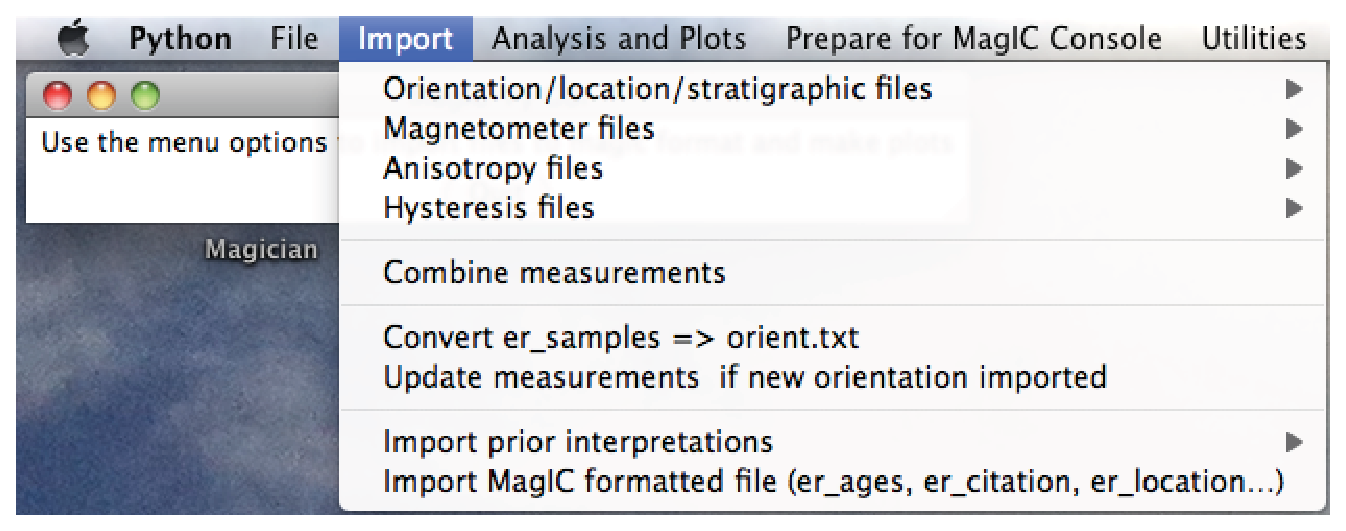
\includegraphics[width=15cm]{EPSfiles/ImportMenu.eps}
%
% \subsubsection{Importing field and sampling information}
% Under the `Orientation/location/stratigraphic files' menu, you will find:
%
%   %\customlink{ImportOrient}
%
% \begin{itemize}
% \item orient.txt format: imports \href{#field\_info}{orient.txt} files by calling the program \href{#orientation_magic.py}{orientation\_magic.py}. The GUI first copies your file into the MagIC Project Directory, presents you with a few forms to fill out and then generates the correct switches for the command line call.
% 	\begin{itemize}
%	\item 	Select orientation file:  choose your orient.txt file from MyFiles
%	\item Select naming convention:  Here you explain the relationship between your sample name and the site name. (see \href{#naming_schemes}{supported naming schemes} for more info).
%	\item Select orientation convention...:  Choose the transformation of your \href{#orientation_schemes}{field convention} to the Lab arrow (the direction of the 'X' arrow used in measurements.  Also, choose whether you want to use the IGRF value calculated by PmagPy for the site latitude, longitude and date,  or you want to supply your own blanket correction to all data in the file.  You can also supply the correct azimuth in the file and perform no further corrections (DEC=0 option).  If the GUI finds sun compass information, it will ask you how many hours to ADD to the time given in the file to get to Greenwich Mean Time (GMT).
%	\item  Select method codes: Choose which \href{#method_codes}{method codes} should be attached to ALL samples.  For example, if they were all drilled in the field, then check 'FS-FD'.
%	\item Update and append...:  If the GUI detects an existing {\it er\_samples.txt} file from a previous import, it will ask if you want to overwrite it (select no) or append to it - note that sample names used before will be overwritten in any case.
%	\end{itemize}
%	The GUI will then generate a call with the appropriate switches and your orientation data will be imported.  NOTE: If you have already combined your measurements files into the master {\it magic\_measurements.txt} file AND you have changed site designations using the site\_name option in the {\it orient.txt} file, you should select ``Update measurements'' to change the site names in that file (these get propagated all the way down the line, so it is important to do this step correctly.
% \item AzDip format:  imports \href{#AZDIP}{AzDip} format files with the \href{#azdip_magic.py}{azdip\_magic.py} program.  Select \href{naming_schemes}{naming convention} and  \href{#method_codes}{method codes} as before.  The orientation is assumed to be the azimuth and plunge of the samples Z direction.  This procedure will only update the {\it er\_samples.txt} file and will not have any location information, so you should convert the er\_samples.txt file created into an {\it orient.txt} file using  the method outlined \href{#samp2orient}{below}, file in the required fields and re-import that into the MagIC directory (be sure to \href{#updatemeas}{update} your measurements file.
%
% %\customlink{IODP_core_summary}
%
%  \item IODP Core Summary csv file: Imports the \href{#LIMS}{IODP} core summary files downloaded from the \href{http://web.iodp.tamu.edu/WTR/html/}{LIMS} database website.
% \item IODP Sample Summary csv file: Imports the \href{#LIMS}{IODP} sample summary file downloaded from the \href{http://web.iodp.tamu.edu/WTR/html/}{LIMS} database website.   This will append to an existing data file, keeping only unique sample names.
% \item Import model latitude data file:  A `model latitude' is a latitude inferred from either inclination data, or some plate tectonic reconstruction.  This file can be used to calculate for example, virtual axial dipole moments (VADMs), or, with the model longitude, a VGP.  Use this option to copy a file with the format:
% er\_site\_name   model\_lat   model\_lon, where the model\_lat is the model latitude and the (optional) model\_lon is the model longitude.  This will be copied into the project directory under the name {\it model\_lat.txt}.
%\end{itemize}
%
%%%
%%% \subsection{Importing magnetometer data}
%%%
%%%When you click on `convert magnetometer files',  you will find a variety of  file formats described in the section on
%%%\href{#magnetometer_files}{magnetometer files}.
%%%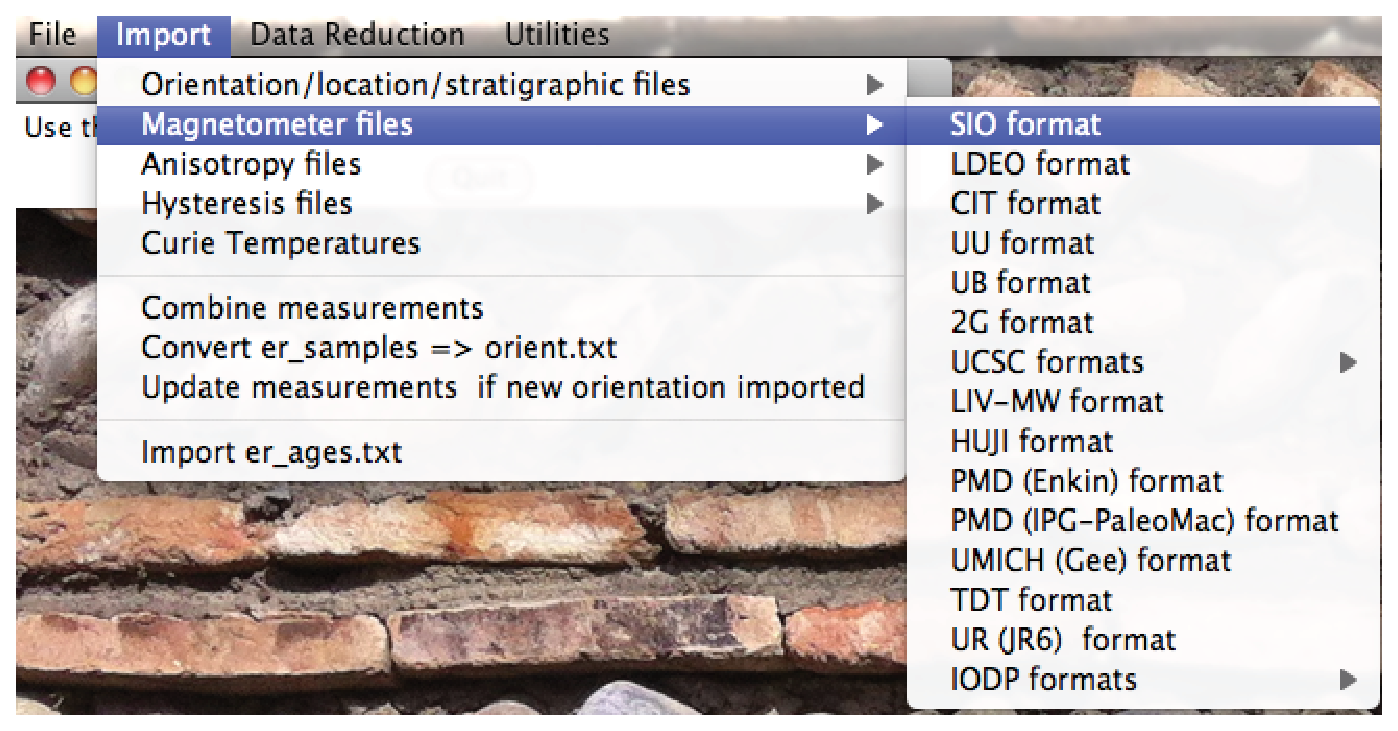
\includegraphics[width=15cm]{EPSfiles/ImportMagnetometer.eps}
%%%Each of these has an idiosyncratic interface.  Some allow importing of entire directories at once, while others import data file by file.   Be sure to \href{#combine_measurements}{combine your measurements} after you finish importing all your measurements, before proceeding to data analysis.
%%%
%%%
%%%%\customlink{SIO}
%%%
%%%\begin{itemize}
%%%\item SIO format:   This option will generate a command line call to the program \href{#sio_magic.py}{sio\_magic.py}.  There are many options for laboratory procedures, naming conventions and so on and the {\bf Pmag GUI} GUI attempts to walk you through the process with as little pain as possible.
%%%	\begin{itemize}
%%%	\item Select \href{#naming_schemes}{naming convention}:  Here you explain the relationship between your sample name and the site name.
%%%	\item Fill in the following information:  Ylou should really really fill in the \href{location_name}{location name} for this file - it will save you time later if you want to upload your data into the MagIC database.  If your specimen/sample relationship is simply to add some characters to te end of your sample name (for example specimen mc144a1 belongs to sample mc144a), fill in the number of characters you use (unless it is '1' as in this case, because that is the default).  If you have some complicated system (for example specimen `\@\#\#\$\%\&\%` belongs to sample `Harry', we can't help you here and you'll have to fill out all the sample names later by hand.  (That should teach you a lesson).
%%%
%%%		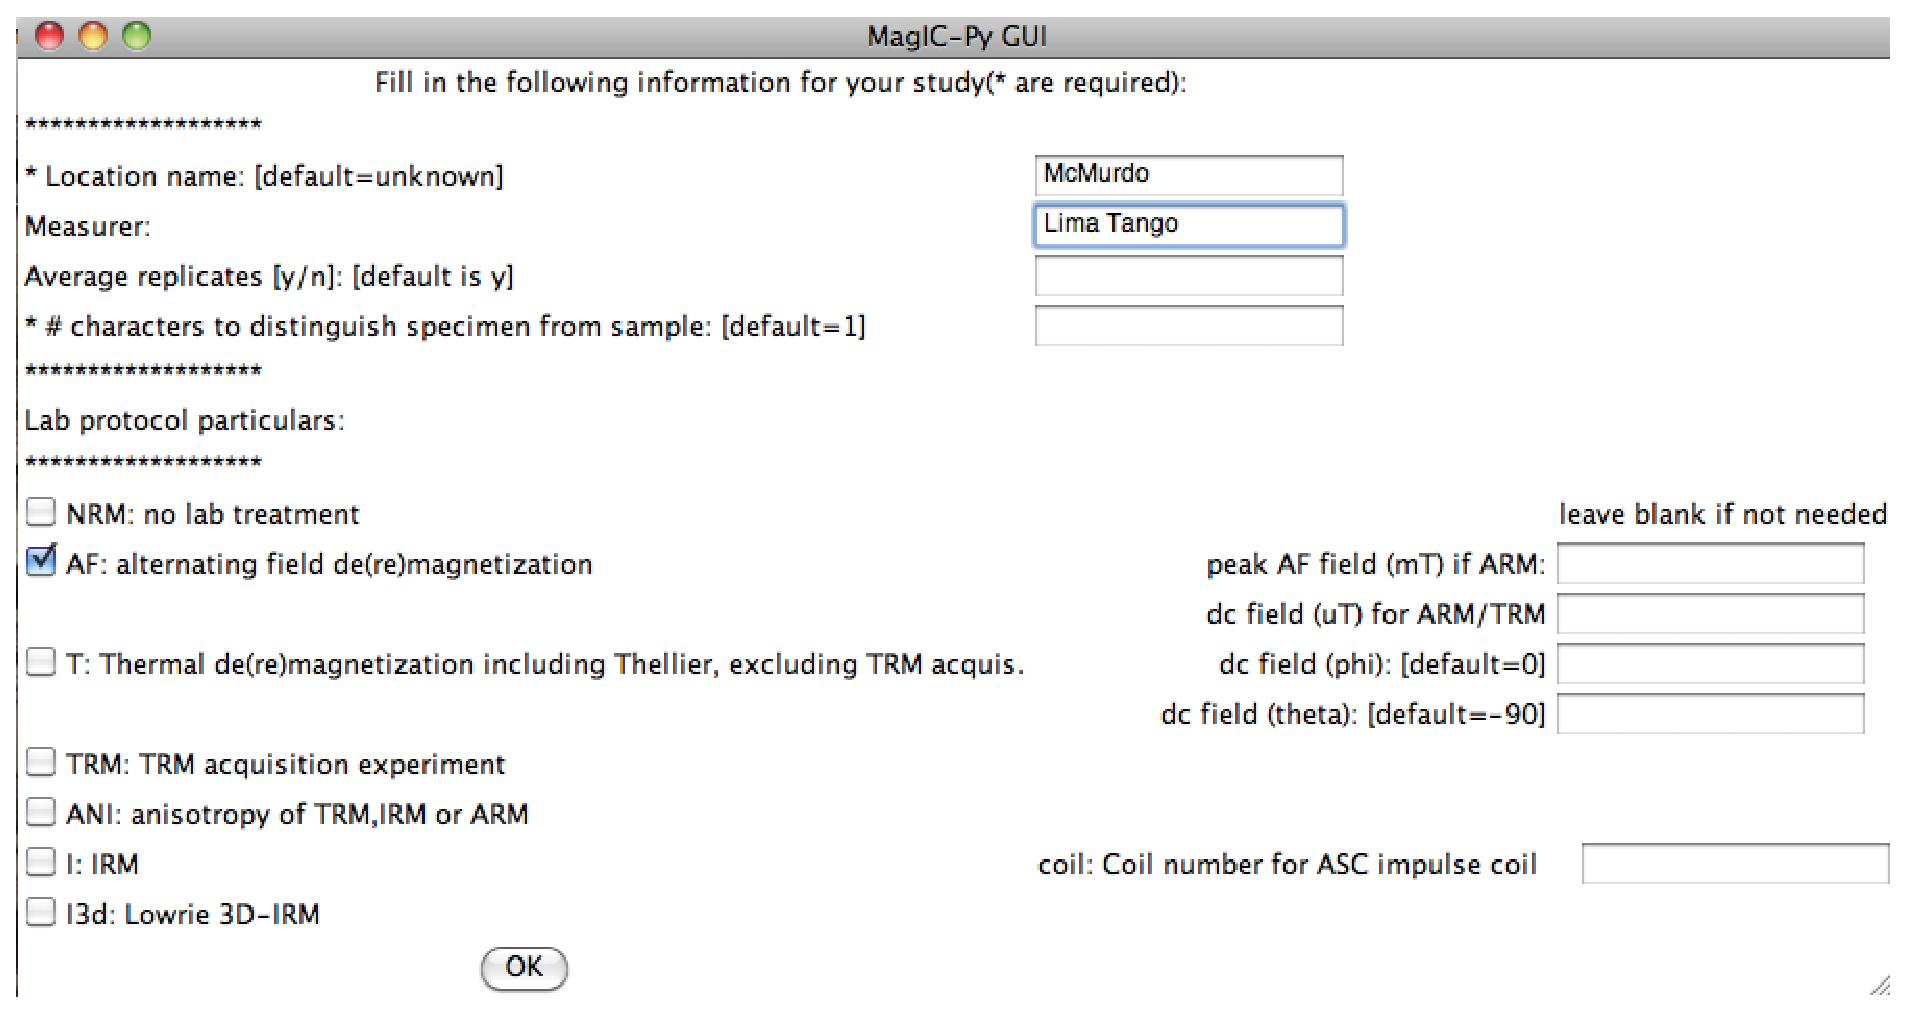
\includegraphics[width=15cm]{EPSfiles/make_sio.eps}
%%%
%%%		You should also check one of the lab protocols you used.
%%%		\begin{itemize}
%%%		\item  If these data were ARMs,  check the AF box and fill in the peak AF and dc field values to the right.  If the lab field direction was not along -Z, then fill in what it was.
%%%		\item  If the data included TRMs from a Thellier or TRM anisotropy experiment, fill in the DC field and orientation (but not the peak AF field.)
%%%		\item If the data were for a TRM acquisition experiment, check the TRM box (but not the 'T' box).
%%%		\item  If these data were part of an anisotropy experiment, check the 'ANI' box and the appropriate AF, T, I box for the type of remanence anisotropy experiment it was.
%%%		\item If the data were IRMs check that box.  If the treatment values were in volts on an ASC impulse coil, give the coil number (1,2, or 3) in the appropriate box.
%%%		\item If the data were part of a Lowrie 3D-IRM experiment (Lowrie, 1990),  \nocite{lowrie90} then check that box.
%%%		\end{itemize}
%%%	\end{itemize}
%%%	\item 2G format:   This import procedure generates calls to \href{#2G_bin_magic.py}{2G\_bin\_magic.py}.  It  differs from that for \href{#SIO}{SIO} formatted in several ways:
%%%	\begin{itemize}
%%%	\item Because 2G  files contain measurements for single specimens, there is usually a directory with many files.  Importing each file individually is painful, so {\bf Pmag GUI}  asks for the directory name and imports ALL files with file endings of .dat or .DAT.
%%%	\item No lab protocol need be specified.
%%%	\item You create an {\it er\_samples.txt} file from the magnetometer file.  For that you should specify at least the orientation method used (e.g., magnetic, sun or sighting), otherwise it is assumed that these are unoriented samples.  The {\it er\_sample.txt} file is very minimalist, having no lithology information, required for a MagIC database contribution.  So after importing the files, you should use the \href{#samp2orient}{Convert samples =$>$ orient.txt} option, file in the required information following the instructions \href{#field_info}{here}, then re-import it into your Project Directory.
%%%	\end{itemize}
%%%
%%%\item LDEO format:  This import procedure is identical to that for \href{#SIO}{SIO} formatted files but generates calls for \href{#LDEO_magic.py}{LDEO\_magic.py}.
%%%\item CIT format:   This format is the `CIT' format used by Craig Jone's {\bf PaleoMag} software package (\url{http://cires.colorado.edu/people/jones.craig/PMag3.html}).   {\bf Pmag GUI} generates calls to the program \href{#CIT_magic.py}{CIT\_magic.py}.       The GUI import option behaves in a similar fashion to the \href{#SIO}{SIO format} import, but you don't specify lab protocol and you can specify method codes.  In the absence of method codes, it is assumed the samples were oriented with magnetic compass.
%%%\item UU format
%%%\item UB format
%%%
%%%\item UCSC formats
%%%\item LIV-MW format
%%%\item HUJI format:  This import procedure is identical to that for \href{#SIO}{SIO} formatted files  but generates calls for \href{#HUJI_magic.py}{HUJI\_magic.py}.
%%%\item IODP format:    This is a pretty simple operation.  Select the file downloaded from the  \href{#LIMS} {LIMS} database and choose whether you want to average replicate measurements or not.  This makes a call to \href{#IODP_csv_magic.py}{IODP\_csv\_magic.py} to do the dirty work.
%%%
%%%\item PMD (Enkin) format:  This import procedure is identical to that for \href{#2G-bin}{2G binary files} except it makes calls to \href{#PMD_magic.py}{PMD\_magic.py}.
%%%
%%%\item UMICH (Gee) format
%%%\item TDT format:  This import procedure is similar to that for \href{#SIO}{SIO} formatted files, generating calls to \href{#TDT_magic.py}{TDT\_magic.py}.  Obviously, you would check the box labelled T and none of the others!   If you want to specify the lab field direction (which may not be parallel to -Z as in the SIO lab, you also have to specify the lab field strength in $\mu$T, even though it is in the file.
%%%\item JR6 format
%%%
%%%\end{itemize}
%%%
%%%
%%%\section{Import menu option}
%%%
%%%Under the Import menu  on the top menu bar, you will find the option of  importing several different kinds of anisotropy data files and hysteresis data.
%%%
%%%%\customlink{ImportAnisotropy}
%%%
%%%\subsection{Importing Anisotropy of magnetic susceptibility data}
%%%
%%%
%%%
%%%
%%%\begin{itemize}
%%%\item \href{#s_magic.py}{The 6 tensor element format (.s)}
%%%\item \href{#KLY4S_magic.py}{LabView program} of Gee et al. 2008: \nocite{gee08}
%%%You first select the KLY4S format input file then the  \href{#naming_schemes}{naming convention}.  After that, input your \href{#location_name}{location name} (strongly encouraged), the measurer (optional), the number of characters to distinguish specimen from sample and the instrument used (optional).    \href{#Combining_measurement_files}{Combine} your measurement files when your are through, to plot versus depth  file or as equal area projections (suitable sample \href{#ImportOrient}{orientation} required).
%%%\item \href{#k15\_magic.py}{15 measurement file format of Tauxe 1998: \nocite{tauxe98}} This import procedure is the same as for the KLY4S file format.
%%%\item \href{#susar4-asc\_magic.py}{SUSAR 4.0 ascii output for Kappabridge}
%%%\item \href{#SUFAR4-asc\_magic.py}{SUFAR 4.0 ascii output for Kappabridge}: This import procedure is the same as for the KLY4S file format.
%%%
%%%\end{itemize}
%%%
%%%%\customlink{ImportHysteresis}
%%%
%%%\subsection{Importing hysteresis data}
%%%
%%%
%%%There are two different modes for importing hysteresis/backfield data:  by file or by directory.  For the former:
%%%\begin{enumerate}
%%%\item Select the file.
%%%\item Select the  \href{#naming_schemes}{naming convention}.
%%%\item Enter the location name, optional measurer, and instrument name, and the specimen name and number of characters to delineate the specimen from the sample.
%%%\item Indicate whether the file is in cgs or SI units and whether this was an IRM backfield experiment
%%%\end{enumerate}
%%%
%%%For importing whole directories:   Your file names must follow the convention described in the section on \href{#Hysteresis_file_formats}{hysteresis file formats}.   Follow the same steps as before, but you will not be asked for a specimen name or whether the data are from backfield experiments as these are supplied by the file names.
%%%
%%%When you are finished importing all the measurement data you need, choose ``Next step''  \href{#Combine}{Step 1. of   Pmag GUI}.
%%%
%%%
%%%
%%%%\customlink{Combining_measurement_files}
%%%
%%%\subsubsection{Combining measurement files}
%%%Each time you import a measurement file, you create a MagIC version of the imported data file with the same name, but a .magic appended to the end.  These filenames are stored in the file {\it measurements.log}.  After you have completed importing all your measurement files, you must combine them together into a single {\it magic\_measurements.txt} file in order to use the other functions in MagIC.py.  Just select this option and everything will be done for you.
%%%
%%%
%%%%\customlink{samp2orient}
%%%
%%%\subsubsection{Creating an orient.txt file from er\_samples}
%%%
%%%
%%%This option makes a call to \href{#convert_samples.txt}{convert\_samples.txt} to convert the {\it er\_samples.txt} file created by some import procedures into an {\it orient.txt} file which can be filled in as desired.  It can be re-imported by \href{#ImportOrient}{importing orientation} information.   After re-importing the orient.txt file, you should update your measurements.
%%%
%%%%\customlink{updatemeas}
%%%
%%%\subsubsection{Update measurements:}
%%%
%%%Update your {\it magic\_measurements.txt} file with new site/location information by calling the program \href{#update_measurements.py}{update\_measurements.py}.  This should be done after \href{#ImportOrient}{importing a new {\it orient.txt} file}.
%%%
%%%
%%%\subsubsection{Importing prior interpretations}
%%%Many people prefer to use the software package that they are familiar with (e.g., \href{#PMD_magic.py}{PaleoMac software of Cogn\'e, 2003)}, \nocite{cogne03}  \href{#CIT_magic.py}{Craig Jones' {\bf PaleoMag} software},  or even previously processed Pmag (Tauxe, 1998) or PmagPy (Tauxe et al., 2010) softare and have generated files containing favorite interpretations of the paleomagnetic data.  MagIC.py can import these interpretation files, allowing the user to skip re-analysis and proceed directly to preparation of files for uploading, or re-interpretation of data files using PmagPy starting with the prior interpretations as a basis.    In any case, the following interpretation files are supported (or could be):
%%%
%%%%\customlink{import_redo}
%%%
%%%\begin{itemize}
%%%\item {PmagPy redo file}:   This option copies the files used by \href{#zeq_redo.py}{zeq\_magic\_redo.py}, \href{#thellier_gui.py}{thellier\_gui.py}  and \href{#thellier_magic_redo.py}{thellier\_magic\_redo.py} and then runs them (see documentation in \href{#mk_redo.py}{mk\_redo.py} for file formats.  This will overwrite any existing interpretation files ({\it zeq\_specimen.txt} or {\it thellier\_specimens.txt}) files you may have created already, so be careful!  Also, this is the main way that the  \href{#thellier_gui.py}{thellier\_gui.py} shares information with the MagIC.py GUI, so import the redo file generated by the auto-interpreter (e.g., {\it thellier\_interpreter\_STDEV-OPT\_redo}  with this option and you will be able to use them within the MagIC.py GUI.
%%%\item DIR:  Not supported at this time $=>$ if desired send example file to {ltauxe@ucsd.edu}
%%%\item LSQ:  Not supported at this time $=>$ if desired send example file to {ltauxe@ucsd.edu}{ltauxe@ucsd.edu}
%%%\item PMM: Not supported at this time  $=>$if desired send example file to {ltauxe@ucsd.edu}
%%%
%%%\end{itemize}
%%%
%%%
%%%%\customlink{ImportMagIC}
%%%
%%%\subsubsection{Copying over your MagIC formatted files}
%%%If you have already some MagIC tables ready,  you can import them into your MagIC folder with this option.  For example, you might have a previous set of specimen interpretations in a {\it pmag\_specimen.txt} file, or age information (in an {\it er\_ages.txt} file.  All age information specific to a give sample or site can be documented in an {\it er\_ages.txt} file (see \url{http://earthref.org/MAGIC/metadata.htm}).  These will be assembled with the respective site/samples in the results table when you \href{#PrepareMagicConsole}{assemble your results}. Other examples might be a location table ({\it er\_locations.txt}) or a citation table ({\it er\_citations.txt}).
%%%
%%% This option will copy your \href{#DataTables}{MagIC} formatted file into the MagIC Project Directory.  Be sure to use the standard file names or the MagIC GUI will ignore them.
%%%
%%%%\customlink{AnalysisPlotsMenu}
%%%
%%%\subsection{Analysis and Plots Menu}
%%%
%%%After you have imported your various datafiles, you can process them using the tools in the \href{#AnalysisPlotsMenu}{Analysis and Plots menu}.    All of these options generate and execute command line calls for various \href{#PmagPy}{PmagPy} programs.  The {\bf MagIC.py} GUI uses default options because it ``knows'' the names of the files it has created, saving you from having to figure that out.   Many of these options require you to type things in on the command line, such as 'a' to s[a]ve plots, 'q' to quit, or simply return to increment the specimen name.  Follow the instructions for the specific program that are printed  in the terminal window   (see also the documentation in the section on \href{#PmagPy}{PmagPy} programs). Once the program has exited, control will be returned to the MagIC.py GUI.
%%%
%%%%\customlink{customize_criteria}
%%%
%%%\begin{itemize}
%%%\item Customize Criteria: here you can change your criteria for acceptance or rejection of data.
%%%		\item Demagnetization Data:  allows you to call  the programs \href{#zeq_magic.py}{zeq\_magic.py} or \href{#demag_gui.py}.  These reads in the {\it magic\_measurements.txt} file created when you \href{#Combining_measurement_files}{combine} your imported  measurement files.  If you have \href{#ImportOrient }{imported orientation} information, it will make the plots using the geographic coordinate system.
%%%		\item Thellier-type experiments:  There are two options here.  The first calls the program \href{#thellier_magic.py}{thellier\_magic.py} and the second calls \href{#thellier_gui.py}{thellier\_gui.py}.  Both  read in the {\it magic\_measurements.txt} file created when you \href{#Combining_measurement_files}{combine} your imported  measurement files.   The {\bf thellier\_gui.py} program works a little differently than the other {\bf PmagPy} programs in that the output interpretations are   not immediately  available to {\bf MagIC.py} when you quit {\bf thellier\_gui.py}.  To use the interpretations, for example from  the auto-interpreter function, you must \href{#import_redo}  import the redo file as described under the Import menu.  You will find the auto-interpreter redo file in the  with the {\it thellier\_interpreter} folder.
%%%		 %\item Microwave experiments
%%%                  \item Equal area:
%%%		\begin{itemize}
%%%			\item Quick look - NRM directions:  This option first fishes out all the NRM measurements from the {\it magic\_measurements.txt} file and stores them in a file called {\it nrm\_measurments.txt}.  The measurement format is then converted to the {\it pmag\_specimen.txt} format using \href{#nrm_specimens_magic.py}{nrm\_specimens\_magic.py}, which also looks for an {\it er\_samples.txt} file and  performs geographic and stratigraphic rotations as available. The GUI will ask for desired coordinate system and level of plotting (by location, site, sample, etc. and then  call the program \href{#eqarea_magic.py}{eqarea\_magic.py} to plot the NRM directions.
%%%			\item General remanence directions:  You are given a choice of tables from {\it pmag\_specimens.txt} up to {\it pmag\_results.txt}, depending on the desired level. You may also choose from among the available coordinate systems and scope of the plot(s) (e.g., location, site, sample).   There are several methods available for estimated confidence bounds for the data set including Fisher, Bingham, Kent or bootstrap.  Plots are made with \href{#eqarea_magic.py}{eqarea\_magic.py}.
%%%			\item Anisotropy data - equal area plots: makes plots with the \href{#aniso_magic.py}{aniso\_magic.py} program.  You can choose the scope of the plot and the method for estimating confidence intervals.
%%%
%%%		\item Hysteresis data:   calls \href{#hysteresis_magic.py}{hysteresis\_magic.py} to plot the data that you  \href{#ImportHysteresis}{imported} and \href{#Combining_measurement_files}{combined} into a {\it magic\_measurements.txt} file.  It generates a file {\it rmag\_hysteresis.txt} with all the hysteresis parameters calculated by the program.  These can be plotted using the 'Hysteresis ratio plots' command.
%%%		\item Hysteresis ratio plots: This calls \href{#dayplot_magic.py}{dayplot\_magic.py} to make plots of hysteresis ratios and the like in the {\it rmag\_hysteresis.txt} file created by \href{#hysteresis_magic.py}{hysteresis\_magic.py}.
%%%		\item IRM acquisition: This calls \href{#irmaq_magic.py}{irmaq\_magic.py} to make plots of IRM acquisition and back field curves.  It uses the {\it magic\_measurements.txt} file created when you \href{#Combining_measurement_files}{combine} your imported  IRM data.
%%%		\item 3D-IRM experiment:   makes plots of the \nocite{lowrie90} 3D-IRM experiment of Lowrie (1990),  \nocite{lowrie90} using the program \href{#lowrie_magic.py}{lowrie\_magic.py}.   It uses the {\it magic\_measurements.txt} file created when you \href{#Combining_measurement_files}{combine} your imported  3D-IRM data and allows the option to normalize the intensity data by the NRM.
%%%		\item Remanence versus depth/height:   makes plots using a call to \href{#core_depthplot.py}{core\_depthplot.py}.  The GUI allows customization of the plot with choice of data type (inclination, declination, etc.), time scale, depth scale, and customization of plot symbols.  If you have imported a \href{#IODP_core_summary}{core summary file}, you can plot the core tops as well.  There is a choice of depth scales with a common depth scale (mcd) as an option.
%%%		\item Anisotropy data versus depth/height:  makes plots using a call to \href{#ANI_depthplot.py}{ANI\_depthplot.py}, reading the {\it rmag\_anisotropy.txt} and {\it magic\_measurements.txt} files in the Project Directory.
%%%		\end{itemize}
%%%		\item Reversals test: performs a bootstrap reversals test with the \href{#revtest_magic.py}{revtest\_magic.py} program.  You can choose coordinate system and selection criteria.
%%%		\item Fold test: performs a fold test with \href{#foldtest_magic.py}{foldtest\_magic.py} and allows choice of selection critieria.  Note - it takes a while so be patient and you need to have \href{#ImportMenu}{imported} structural corrections.
%%%
%%%\end{itemize}
%%%
%%%%\customlink{PrepareMagic}
%%%
%%%\subsection{Prepare for MagIC}
%%%Once all your data have been imported and interpreted using one of the interpretation tools outlined in the section on \href{#AnalysisPlotsMenu}{Analysis and Plots}, you can assemble the results into the various \href{#DataTables}{tables} expected by MagIC, e.g., the {\it pmag\_specimens, pmag\_samples, pmag\_sites} and {\it pmag\_results} tables (also various rock magnetic tables, if available).
%%%\begin{itemize}
%%%		\item Assemble specimens: The various programs for interpreting measurement data like \href{#zeq_magic.py}{zeq\_magic.py} or \href{#thellier_magic.py}{thellier\_magic.py} produce {\it pmag\_specimens.txt} formatted files with names like {\it zeq\_specimens.txt} or {\it thellier\_specimens.txt}.  The directional data should be recalculated for various coordinate systems and the intensity data corrected for anisotropy corrections and the like.  All of these data need to be assembled into a single {\it pmag\_specimens.txt} file, which is what this option does.
%%%
%%%		%\customlink{AssembleResults}
%%%
%%%		\item Assemble results:   After assembling the specimen data into a single {\it pmag\_specimens.txt} file, data must be averaged by sample and/or by site and stored in {\it pmag\_sample.txt} and {\it pmag\_site.txt} tables.  The directional data can be converted to VGPs and intensities into V[A]DMs, which are kept in the {\it pmag\_results.txt} table. Study level averages such as paleomagnetic pole positions can be calculated.  All of these operations are carried out by the program \href{#specimens_results_magic.py}{specimens\_results\_magic.py}.
%%%		\begin{itemize}
%%%			\item You have a choice of selection criteria (default, existing (created with the \href{#customize_criteria}{customize criteria} option, and none).
%%%			\item For many applications, data are normally averaged first by sample, then by site and this is the default.  But and argument could be made that in certain circumstances (e.g.,  with intensity data in which each specimen is independent of the other), site averages could be made using all the specimen data together and not averaging by sample.  Choose  -aD to average directions by site and not by sample and -aI to average intensities by site and not by sample. Also, choose -sam to calculate sample level VGPs and VADMs if desired. Otherwise, the program will do this for site level data onlly.
%%%			\item For calculating VDMs, you need oriented inclinations and for VADMs, you need a latitude.  The latitude can be the present latitude or a reconstructed paleolatitude (model latitude).  To choose the present latitude, select '-lat' or \href{#ImportMenu}{import} a model latitude file and choose that option.
%%%			\item  The -p option lets you  look at the data site by site to check if there are terrible errors.  If you want to reconsider some of the sample orientations, for example, you should use the option in the \href{#Utitlities}{Utitlities menu} to check the sample orientations for common mistakes.
%%%			\item You can just skip the directional (-xD) or intensity (-xI) calculations if they are not relevant (this speeds things up a bit).
%%%			\item If you want to calculate normal and reverse means for the study, select -pol.
%%%			\item You can choose which coordinate systems you want to include in the MagIC tables. The GUI sniffs through the options and presents them to you.
%%%			\item The MagIC database wants all non-synthetic data to have ages associated with them.  Site/sample specific ages are entered using the {\it er\_ages.txt} table (imported in the {Import er\_ages option} in the \href{#er_ages}{Import Menu}, but age bounds for the study must be entered so that \href{#specimens_results_magic.py}{specimens\_results\_magic.py} can assign age bounds for every result.   The GUI therefore asks for these age bounds.   Age units are a controlled vocabulary, so choose from this list:  [Ga, ka, Ma, years AD (+/-), Years BP, Years Cal AD (+/-) Years Cal BP].   If you enter nothing, the default age bounds will be 0 to 4.5 Ga.
%%%		\end{itemize}
%%%		\item Prepare upload txt file:  The \href{http:earthref.org/MAGIC/search-beta}{MagIC Website} will import a specially formatted ascii file, parsing all the tables into their niches.  Choosing this option will create an {\it er\_locations.txt} file for you based on what is in the {\it er\_sites.txt} file.  It will ask you for the missing required information.  Then the GUI prepares a file called {\it upload.txt} which can be directly imported into the MagIC database and attached to the associated reference.
%%%\end{itemize}
%%%
%%%
%%%
%%%
%%%%\customlink{Utilities}
%%%
%%%\subsection{Utilities Menu}
%%%
%%%\begin{itemize}
%%%		\item Check sample orientations:  This program calls the program \href{#site_edit_magic.py}{site\_edit\_magic.py}.  It steps through the data site by site and allows you to evaluate orientation information, testing outliers against specific, common field mistakes (arrow wrong direction, wrong scratch mark, etc.)
%%%		\item Extract Results to table for publication:  After assembling your results, you can extract information from the {\it pmag\_results.txt} file as an tab delimited (excel ready) file or as a (my favorite) LaTex formatted table.  That way, the data in your publication will be identical to the data in the MagIC database (what a concept!).  This option allows you to do that using the program \href{#pmag_results_extract.py}{pmag\_results\_extract.py}.  It will create two files:  {\it Intensities.txt} and {\it Directions.txt}.
%%%		\item Map of VGPs:  makes plots using \href{#vgpmap_magic.py}{vgpmap\_magic.py}, which reads from the {\it pmag\_results.txt} file (where VGPs are stored).  To get VGPs, you need to \href{#AssembleResults}{assemble} your results first.   If you \href{#ImportMenu}{imported} orientation data, you can select the coordinate system.  You can also choose whether or not to `flip' the reverse VGPs and the location of the 'eye' in the orthographic plot.
%%%		\item Map of site locations: makes plots using \href{#basemap_magic.py}{basemap\_magic.py} which reads from the {\it er\_sites.txt} file.  Choosing high resolution requires that the  \href{#HighRes}{high resolution} datafiles be installed.  There are many more options available if you use the program on the command line - this is just for a `quick look'.
%%%
%%%\item Make IZZI exp. chart: The IZZI paleointensity experiment (Tauxe and Staudigel, 2004) \nocite{tauxe04} is a complicated protocol which requires some concentration to get the order of heating steps in the right order.  This utility calls \href{#chartmaker.py}{chartmaker.py} to make a chart to facilitate the laboratory procedure.
%%%\item Expected directions/paleolatitudes:  calls \href{#apwp.py}{apwp.py} to calculate paleodirectiions and paleolatitudes for a give location at a specified time, after assigning it a tectonic plate.
%%%\end{itemize}
%%%
%%%\subsection{Help Menu}
%%%
%%%Takes you to this Cookbook.


\customlink{magic_gui.py}

\chapter{MagIC GUI Tutorial}
\label{chap:MagIC GUI}

{\bf MagIC GUI} is a Graphical User Interface written by Lori Jonestrask.  It is meant for efficiently compiling a contribution for uploading to the MagIC database.  MagIC GUI is specifically designed for making a contribution without measurement data; if you ARE including measurement data, we recommend that you use \href{#pmag_gui.py}{Pmag GUI} instead.
MagIC GUI allows you to add data at the location, site, sample, and specimen levels.  You can also add results and ages.  The program uses an Excel-like grid interface for entering and editing data.  Useful features include: pop-up menus with controlled vocabularies, multi-cell pasting from external spreadsheets, and built-in validations for MagIC database requirements.  


\section{Starting with MagIC GUI}
Start up MagIC GUI.  You'll do this by clicking on the icon (if you downloaded the \href{#standalone}{standalone} version) or entering `magic\_gui.py' on your \href{#command_line}{command line} (if you downloaded the full PmagPy installation). 
  
When you first start {\bf magic\_gui.py}, you will change directories into a  `Project Directory'. For each study, create a directory with a name that relates to that study. Here we will call it {\it MyProject}.  This is where you will collect  and process all the rock and paleomagnetic data for a given study, usually a publication.   The project directory name should have NO SPACES and be placed on the hard drive in a place that has NO spaces in the path. Under certain Windows versions, this means you should not use your home directory, but create a directory called for example: D:$\backslash$MyPmagProjects and put {\it MyProject} there.

  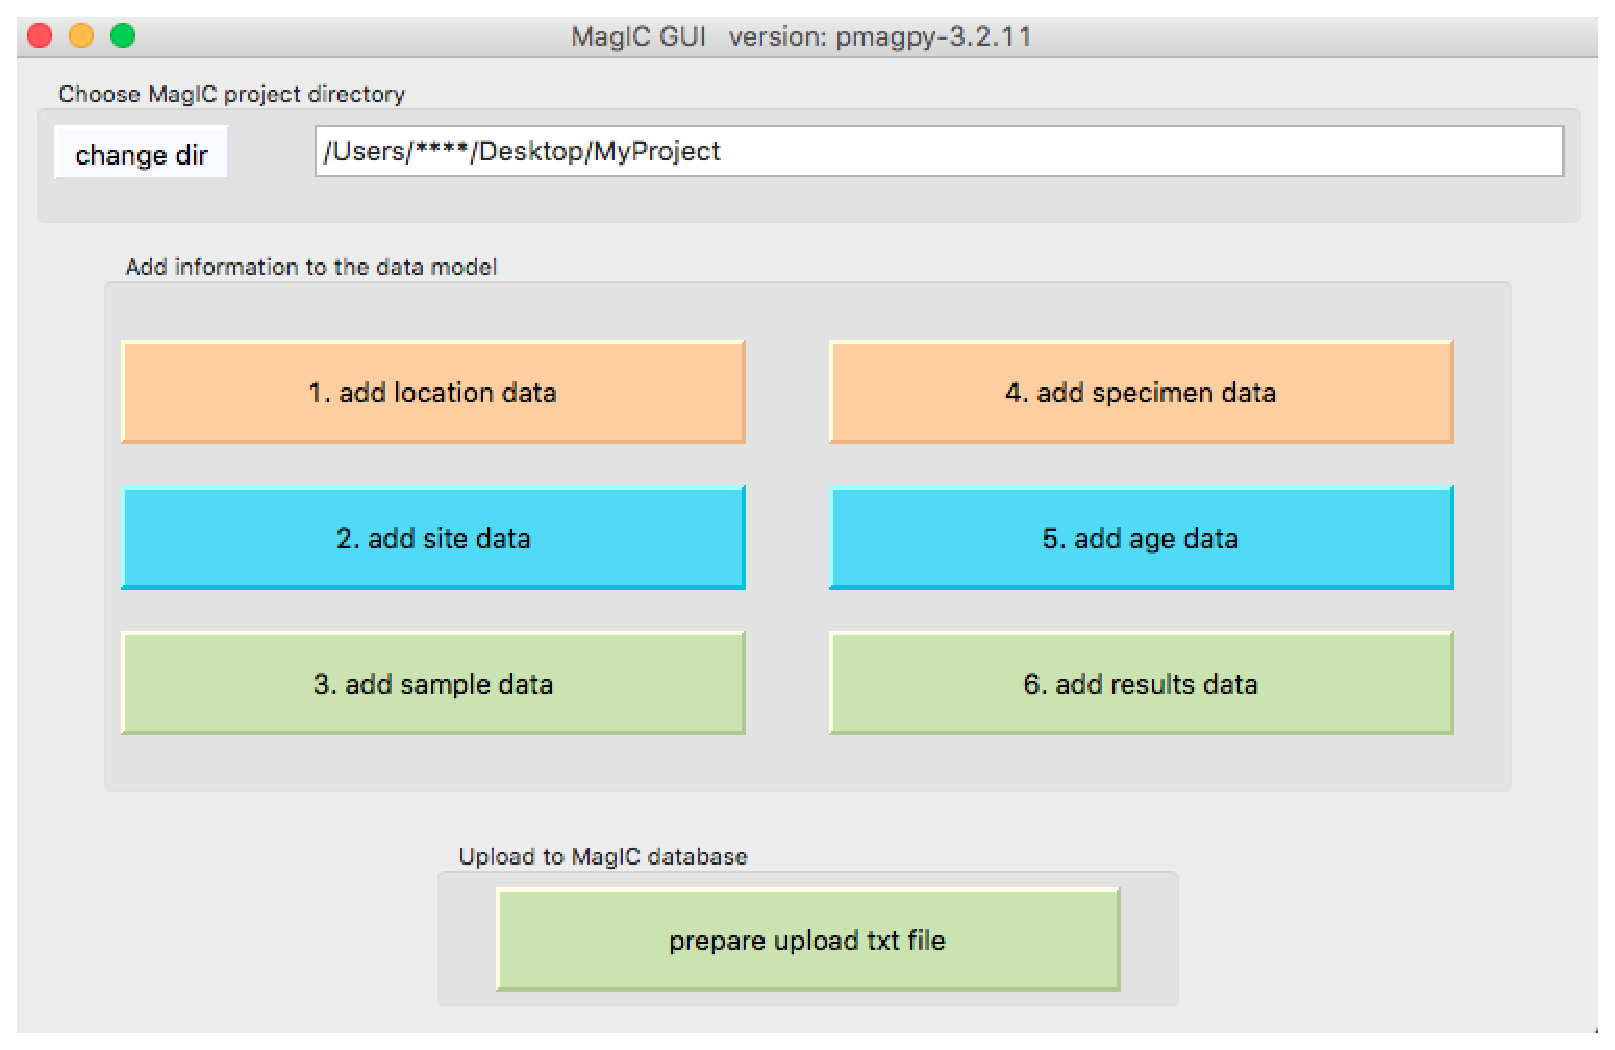
\includegraphics{EPSfiles/MM_main_frame.eps}
  
\section{MagIC GUI example dataset}
Now we'll walk through a simple data input process, with fake data.
  \begin{itemize}
  \item Start by clicking on `1. add location data'.  Enter location data as seen below. Notice use of the context menu: in most instances, these will provide controlled vocabularies.
    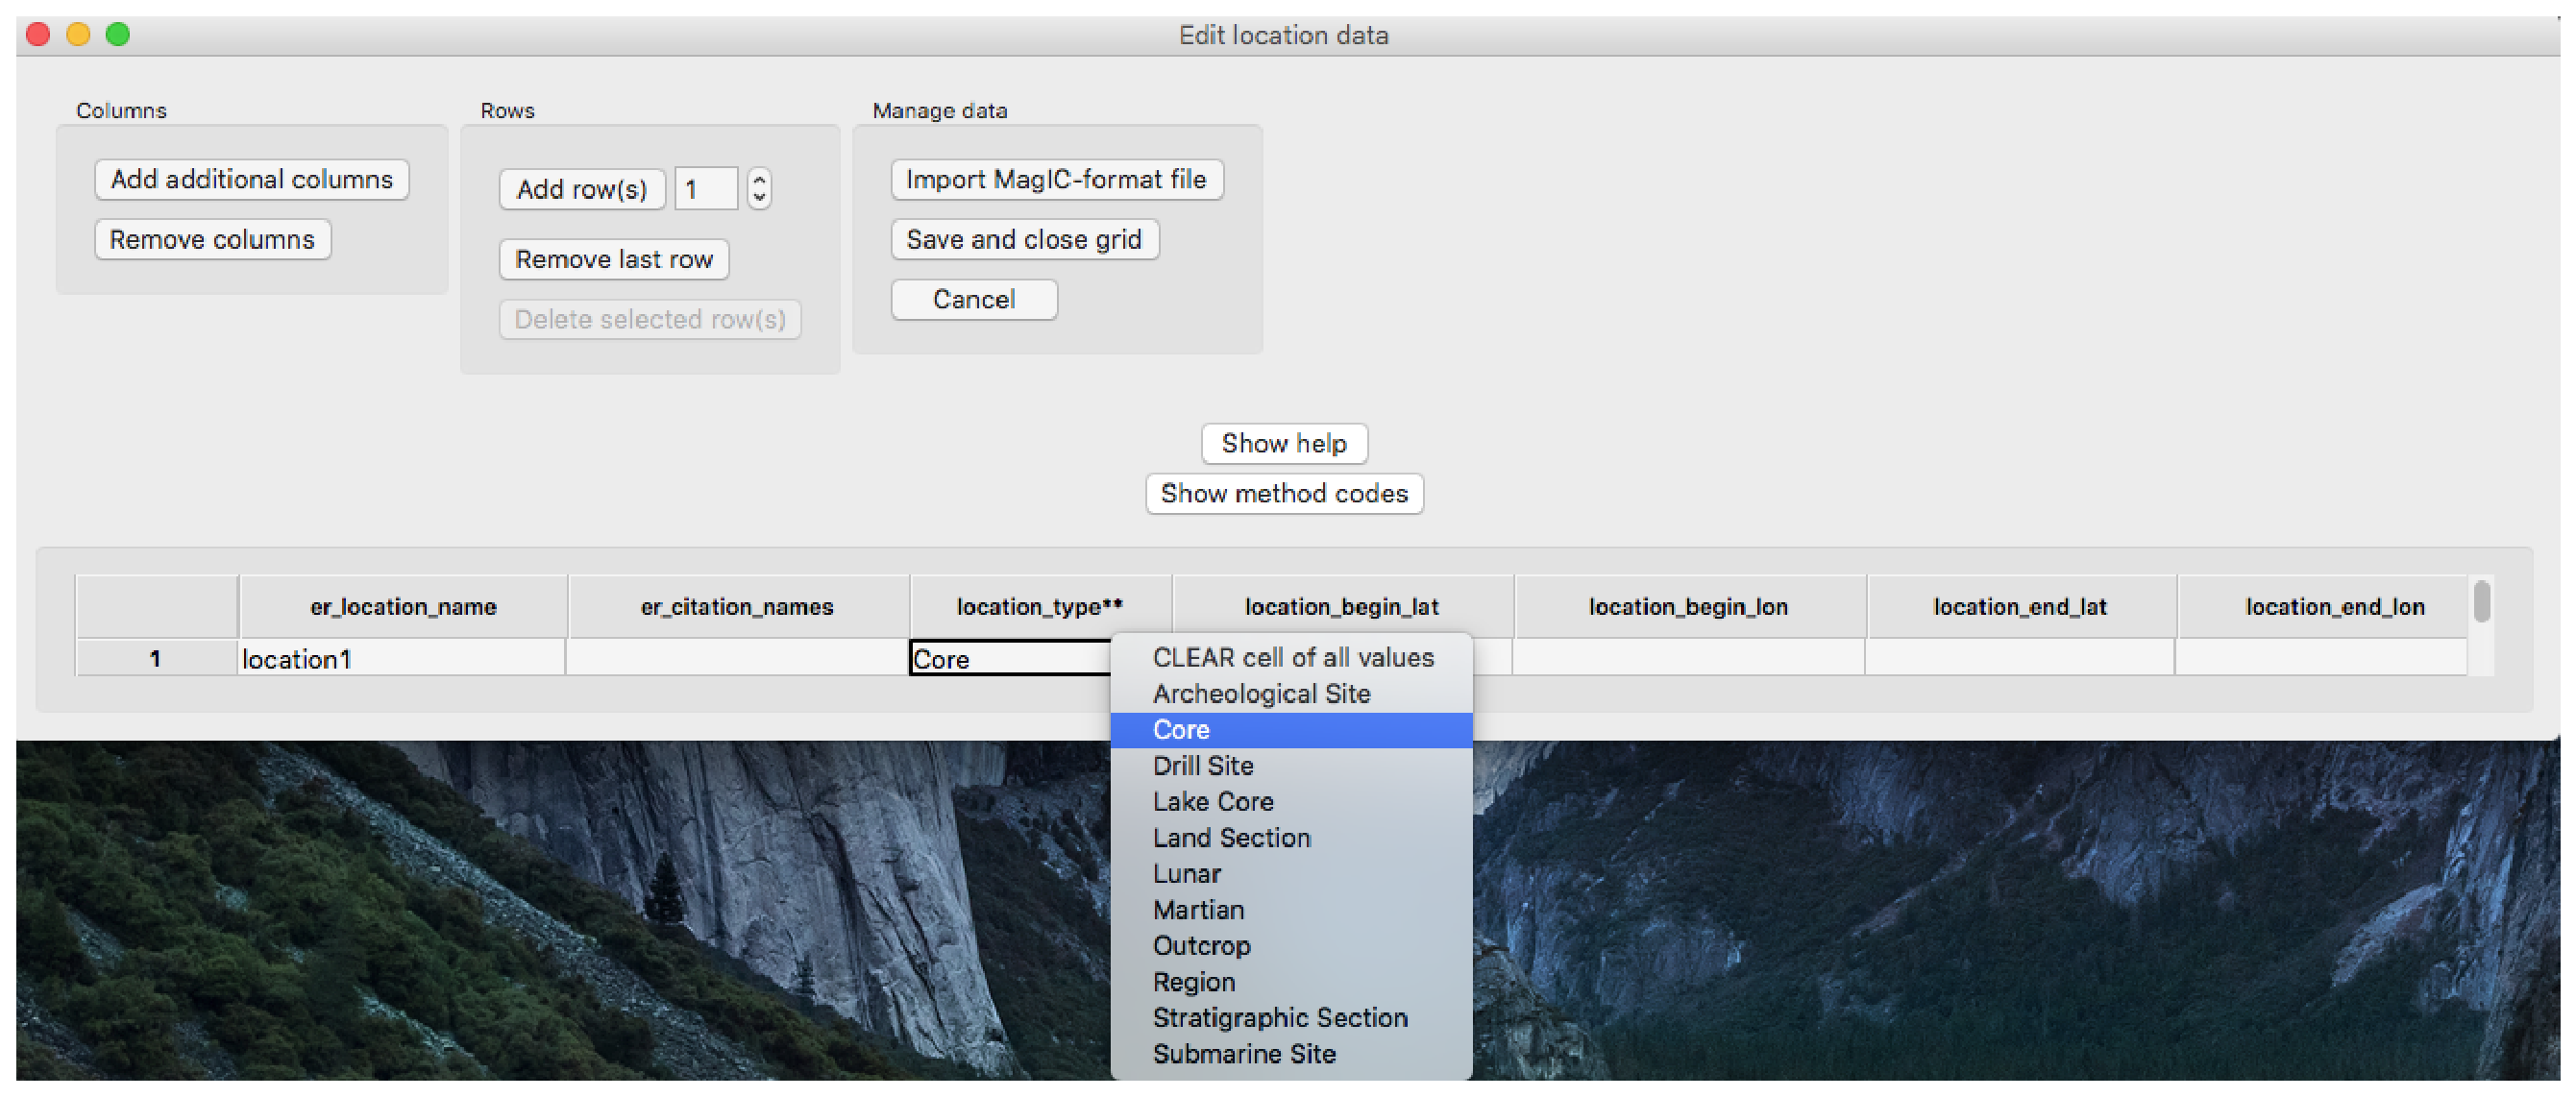
\includegraphics{EPSfiles/MM_location_grid_with_menu.eps}
  \item You'll notice that some information is not filled in.  First, if you have no outside citations, you can leave `er\_citation\_names' blank and it will be automatically filled in with `This study' after you save this data.  Second, if you will be providing latitude/longitude for sites, then you don't need to provide it at the location level.  The program will extract start and end latitude and longitude from your site data and apply it to each location.  
  \item If you want to provide more than the default required information, you may want to add more columns to your grid.  In our case, we'll add in `Country'.  To do this, just click the button `Add additional columns'.  Choose whatever headers you want to add and select `Ok'.
    
    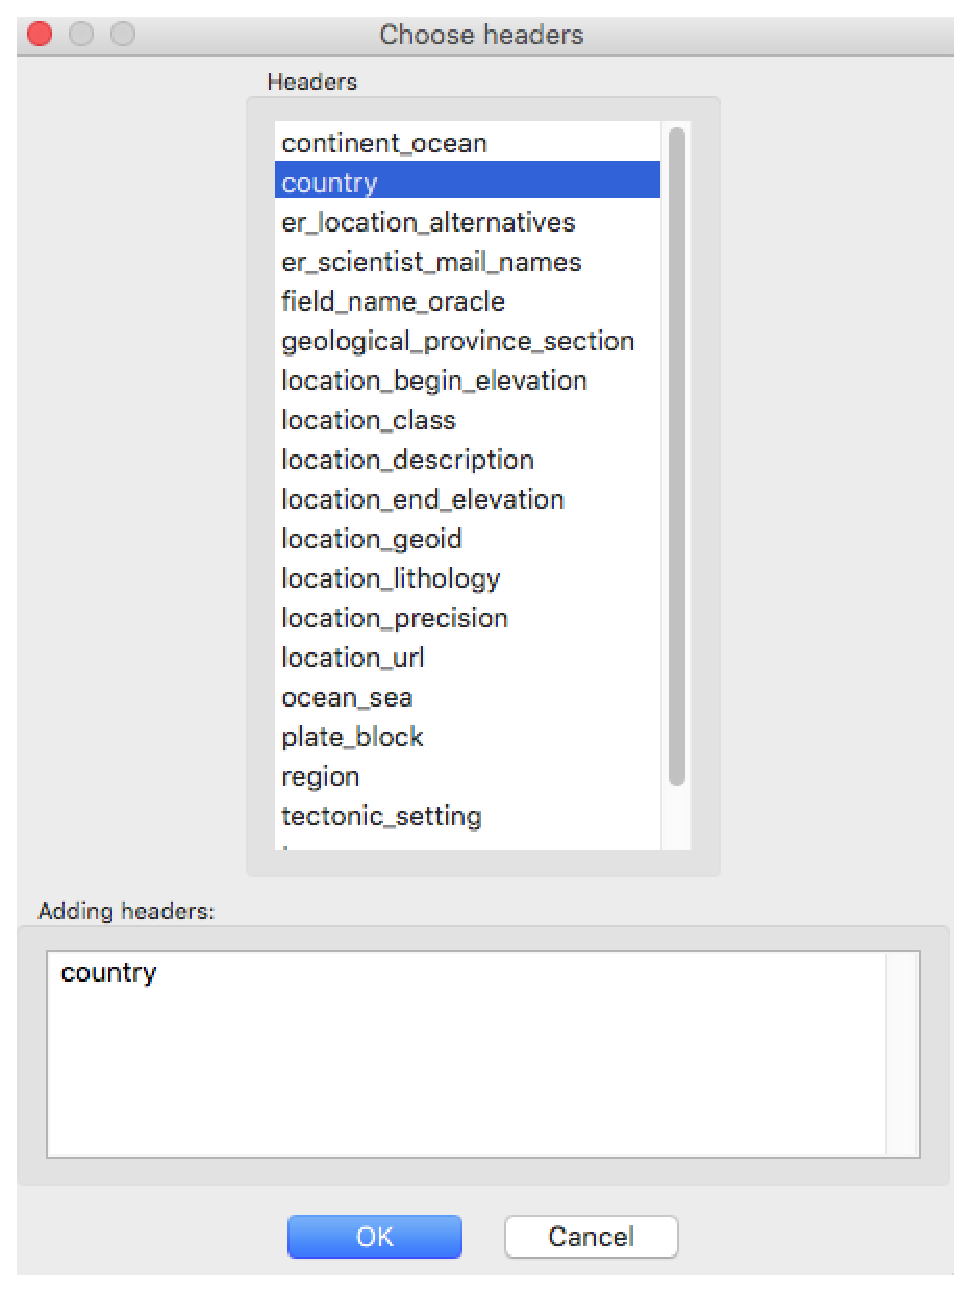
\includegraphics{EPSfiles/MM_add_location_headers.eps}
    
  \item Now you'll have a new column with a new controlled vocabulary.  Find and select `U.S.A.'.  When you're done entering location data, click `Save and close grid'.
    
  \item Next, we'll add in sites, so start by opening the site grid.  We will have two sites in this dataset, so click the `Add row(s)' button once.  Then, fill in the grid.  For some of the values, both sites will have the same value.  To provide this data more efficiently, click on the column label to edit all values in that column.  If that column has a menu, you can then click anywhere in that column and make a selection for every cell in the column. Once you're done editing the column, click the header again to exit the multiple-cell-edit mode.
    
    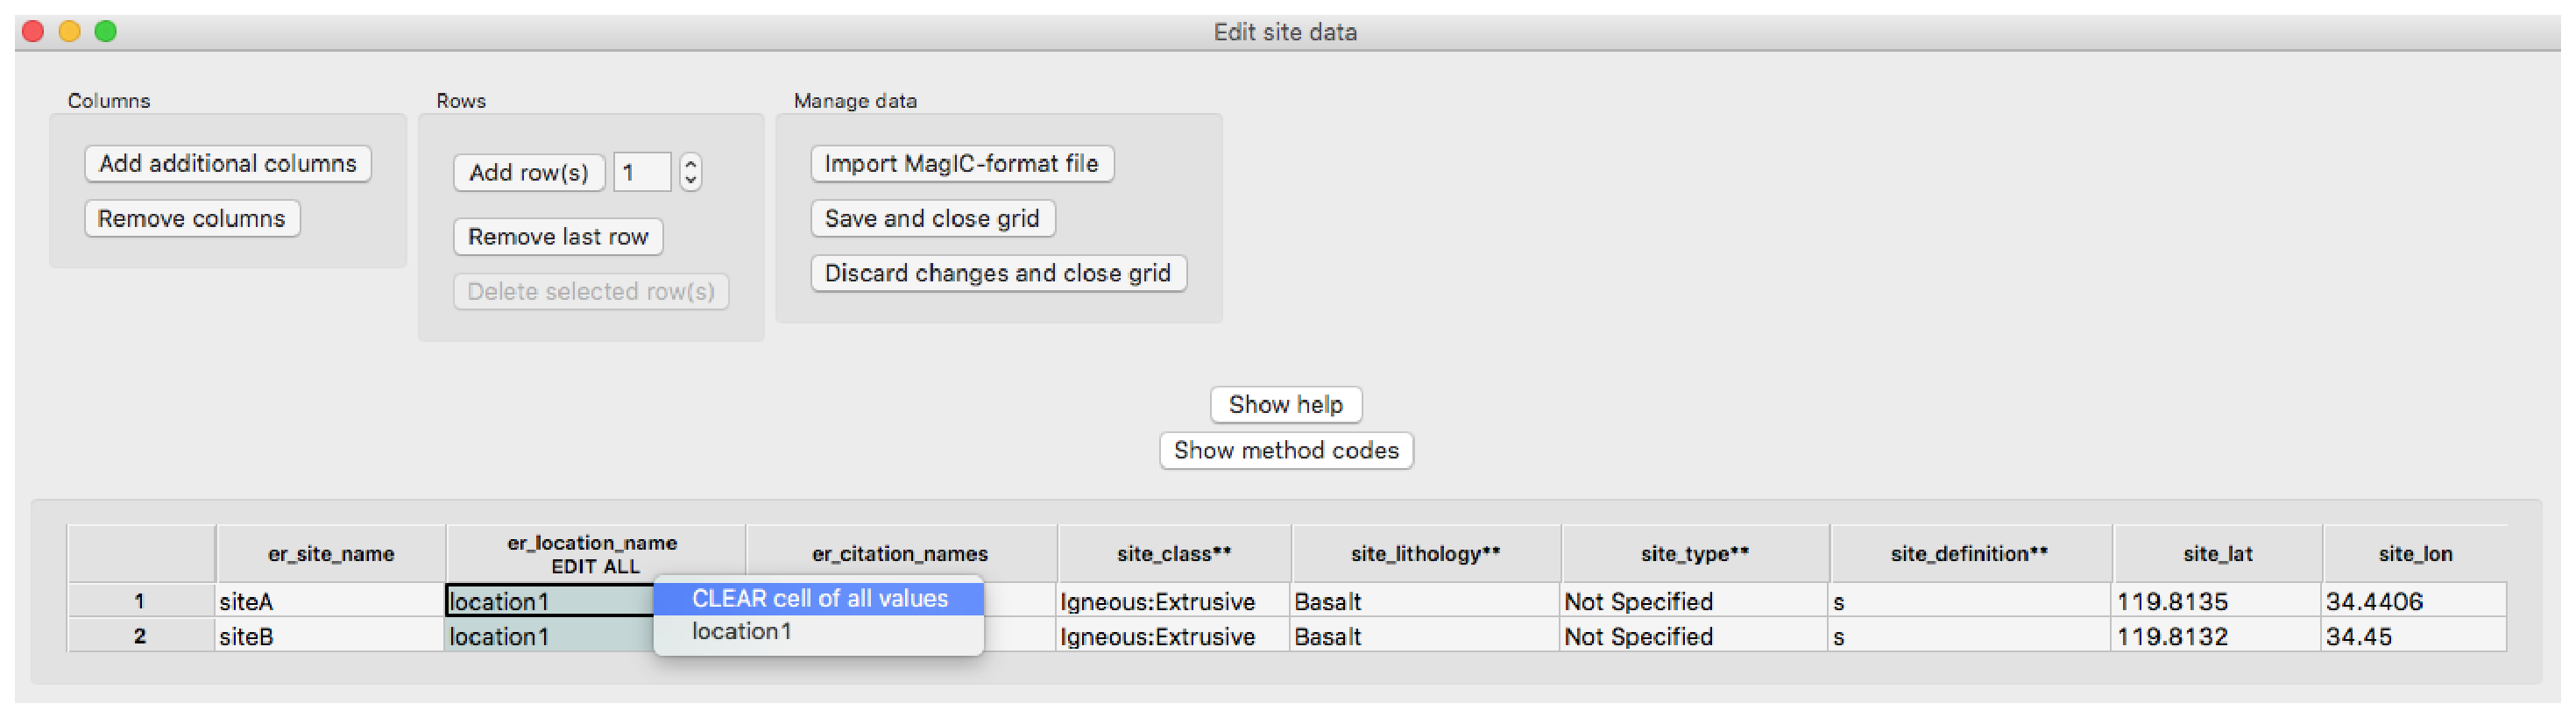
\includegraphics{EPSfiles/MM_site_grid_with_edit_all.eps}
    
  \item Once you're done adding sites, save and close the site grid, then open the sample grid.
    Enter data as you see below:
    
    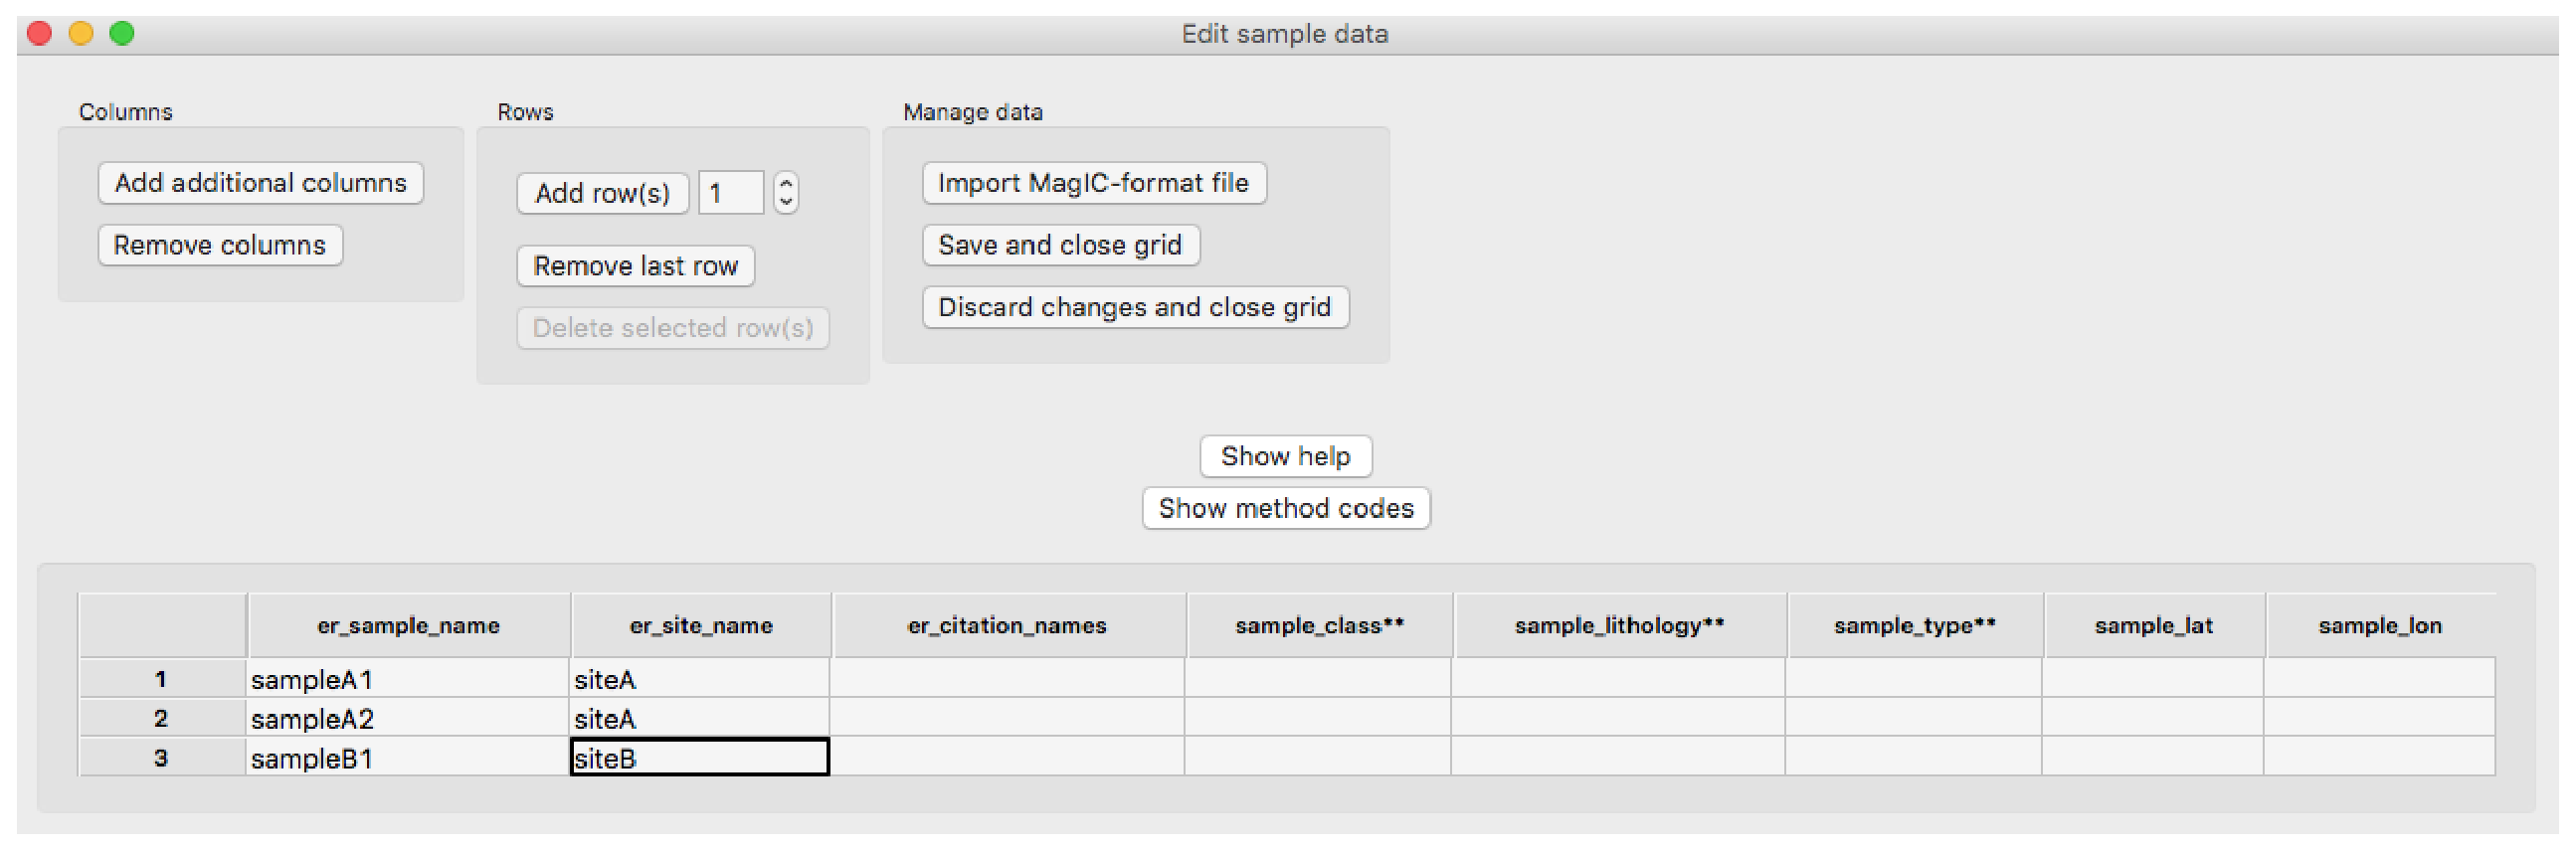
\includegraphics{EPSfiles/MM_sample_grid.eps}
    
    All other required data will fill in automatically.  If you don't provide latitude and longitude data for a sample, it will propagate down from the site after you save and close the grid.
    
  \item For samples, we will add an additional statistic.  Click 'Add additional columns' and select `sample\_int\_sigma' from the 'Headers for interpretation data' column.  Select 'ok' and have a look at your new grid.  You'll notice that the column you selected has been added, as well as two additional columns: `magic\_instrument\_codes' and `magic\_method\_codes++'.  These two columns are required if you are including any interpretation data at the sample level.  Fill in the added columns.  You'll notice that `magic\_method\_codes++' has a drop-down menu.  If you aren't familiar with the MagIC codes system, click `Show method codes' which provides brief explanations for each possible code.
    
    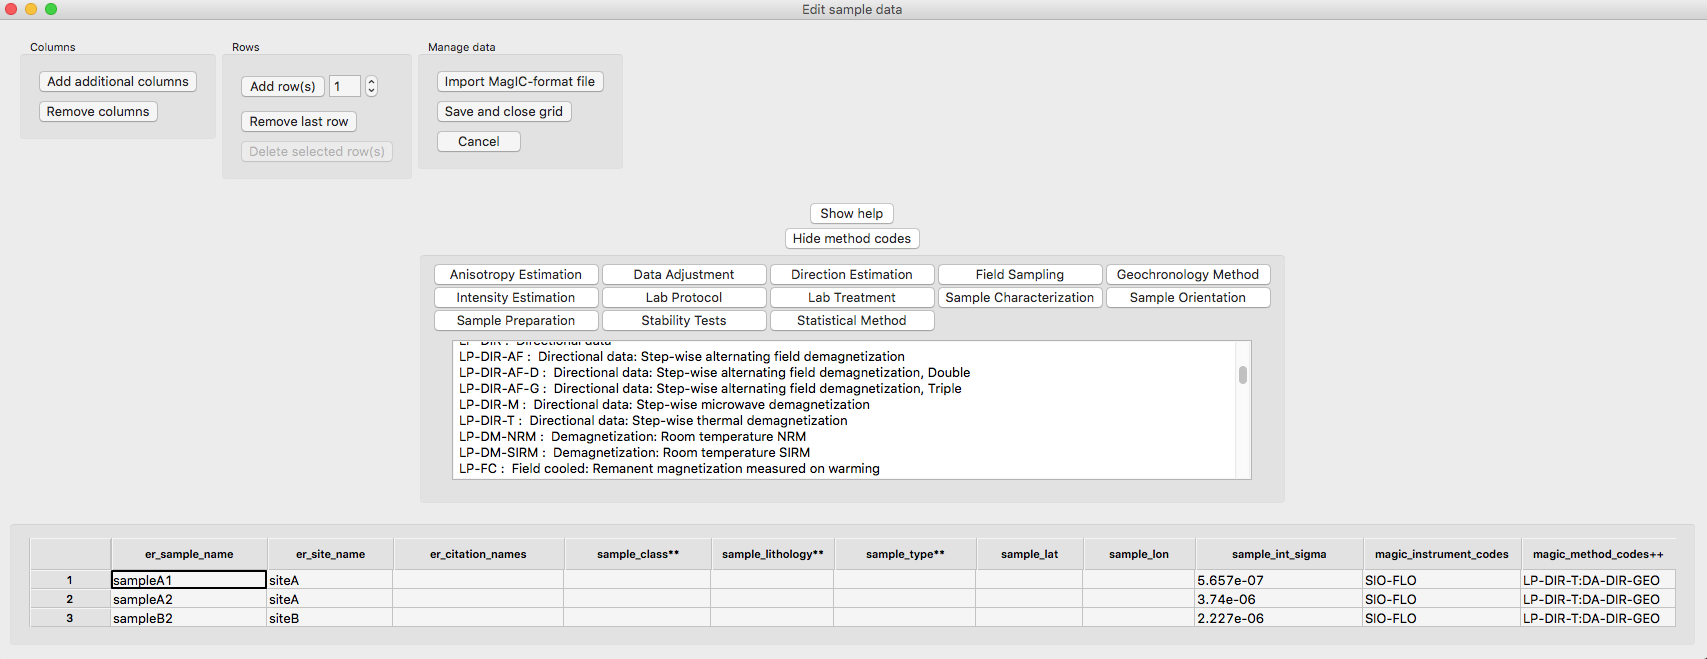
\includegraphics{EPSfiles/MM_sample_grid_added_cols.eps}
    
  \item Save and close the sample grid, then re-open it to see how the data have propagated (re-opening the grid isn't necessary for the program, this is just for you to see what MagIC GUI does automatically).
    
    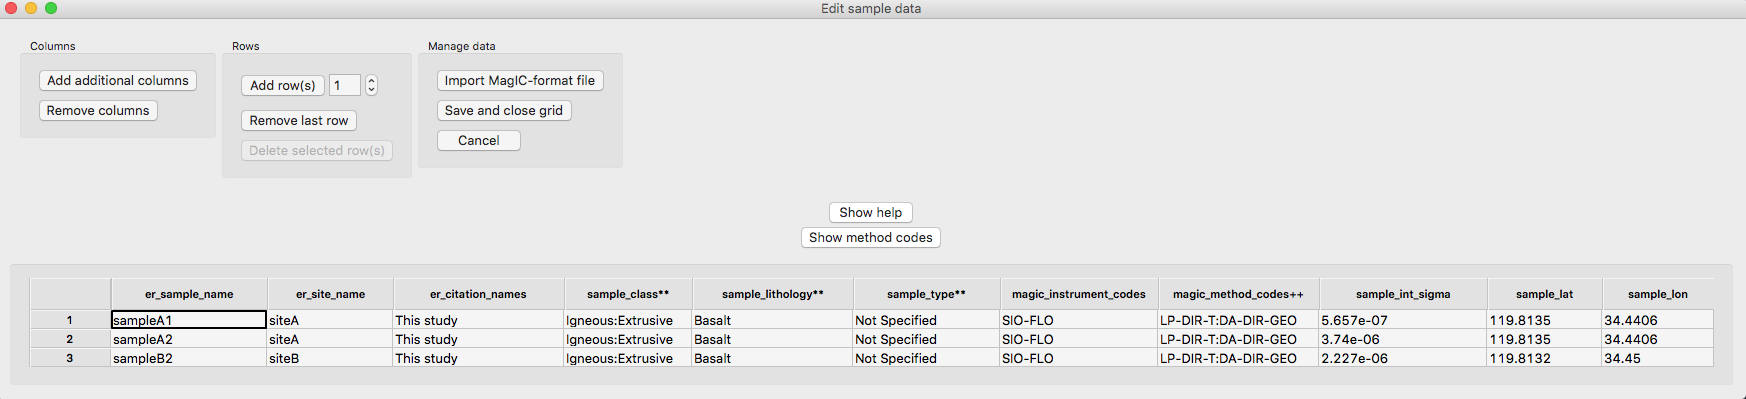
\includegraphics{EPSfiles/MM_sample_grid_propagated_full.eps}

  \item In this example, we won't add data at the specimen level, so we will be skipping step 4.  Adding specimens works just the same as adding samples.
    
  \item Now open the age grid.  You can assign ages at any level, at multiple levels, or at no level.  For this study, we will add ages at the sample level.  Choose sample as the age level.  Next, you'll need to add in the `age' column.  Fill in the grid as below:

    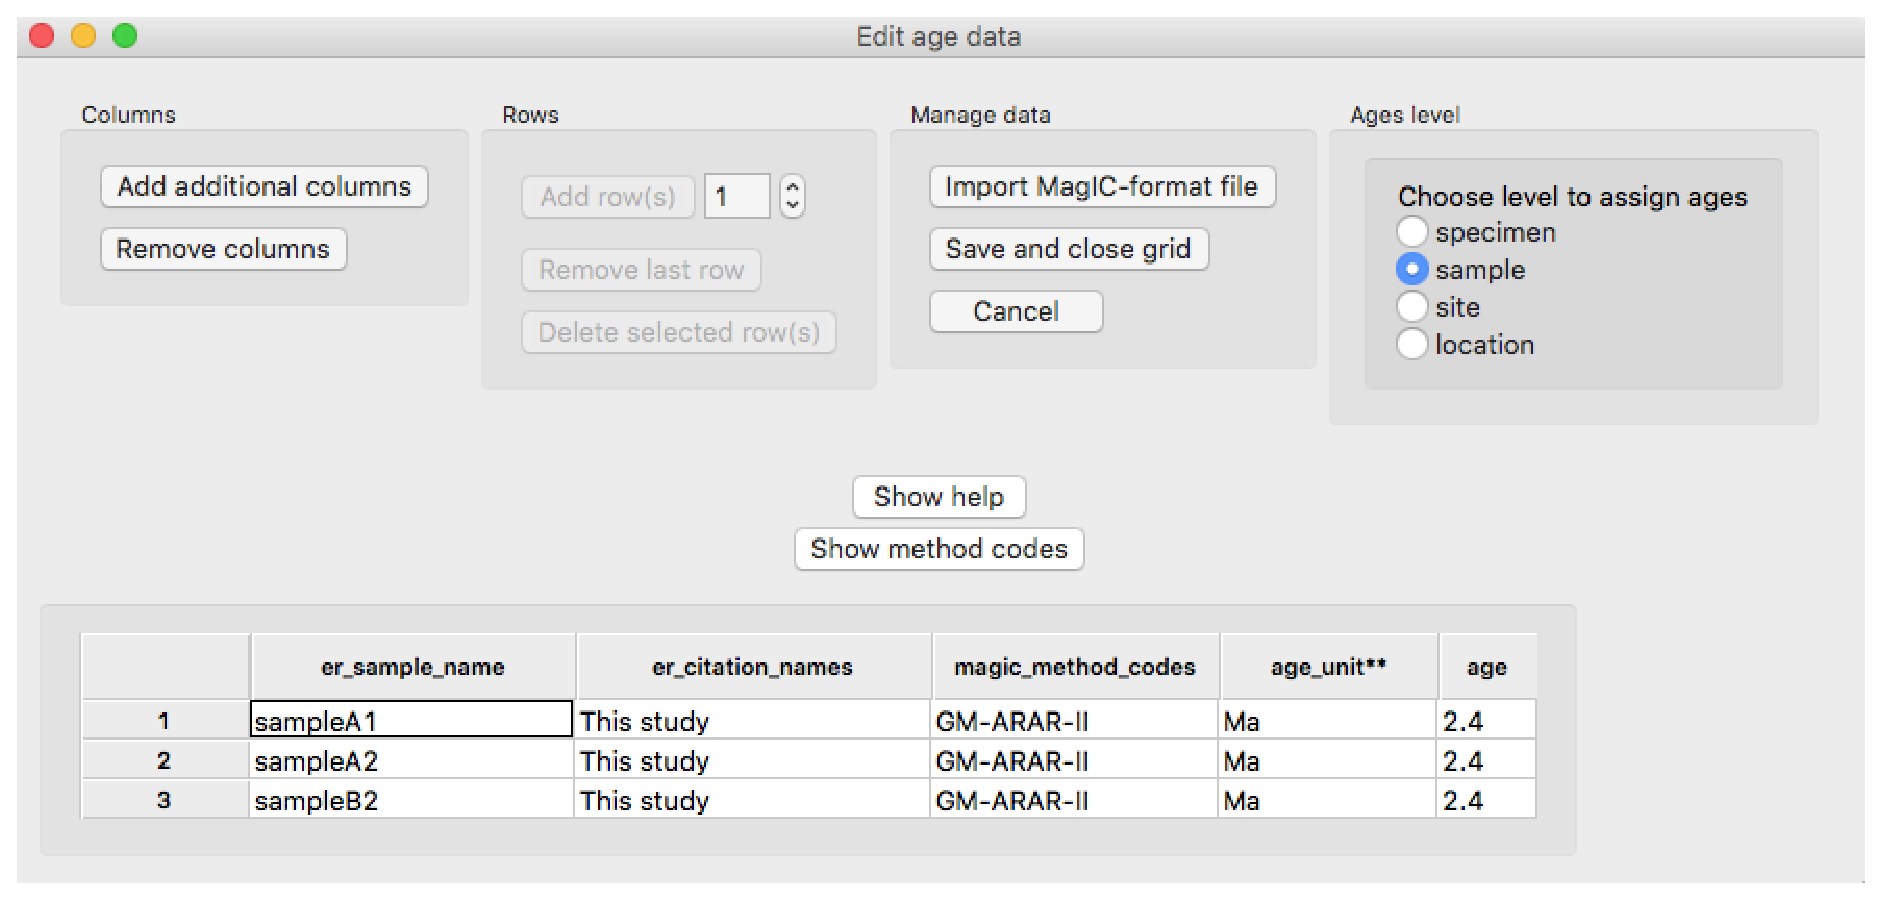
\includegraphics{EPSfiles/MM_age_grid.eps}

  \item You'll notice that you can't add or remove rows in this grid.  If you want to add an additional sample, you would need to go back to the sample grid to do so.

  \item The last data step is to put in result information.  You'll need to open the result grid and, for this example, add just one statistic: `vadm'.  Then, fill out the grid:

    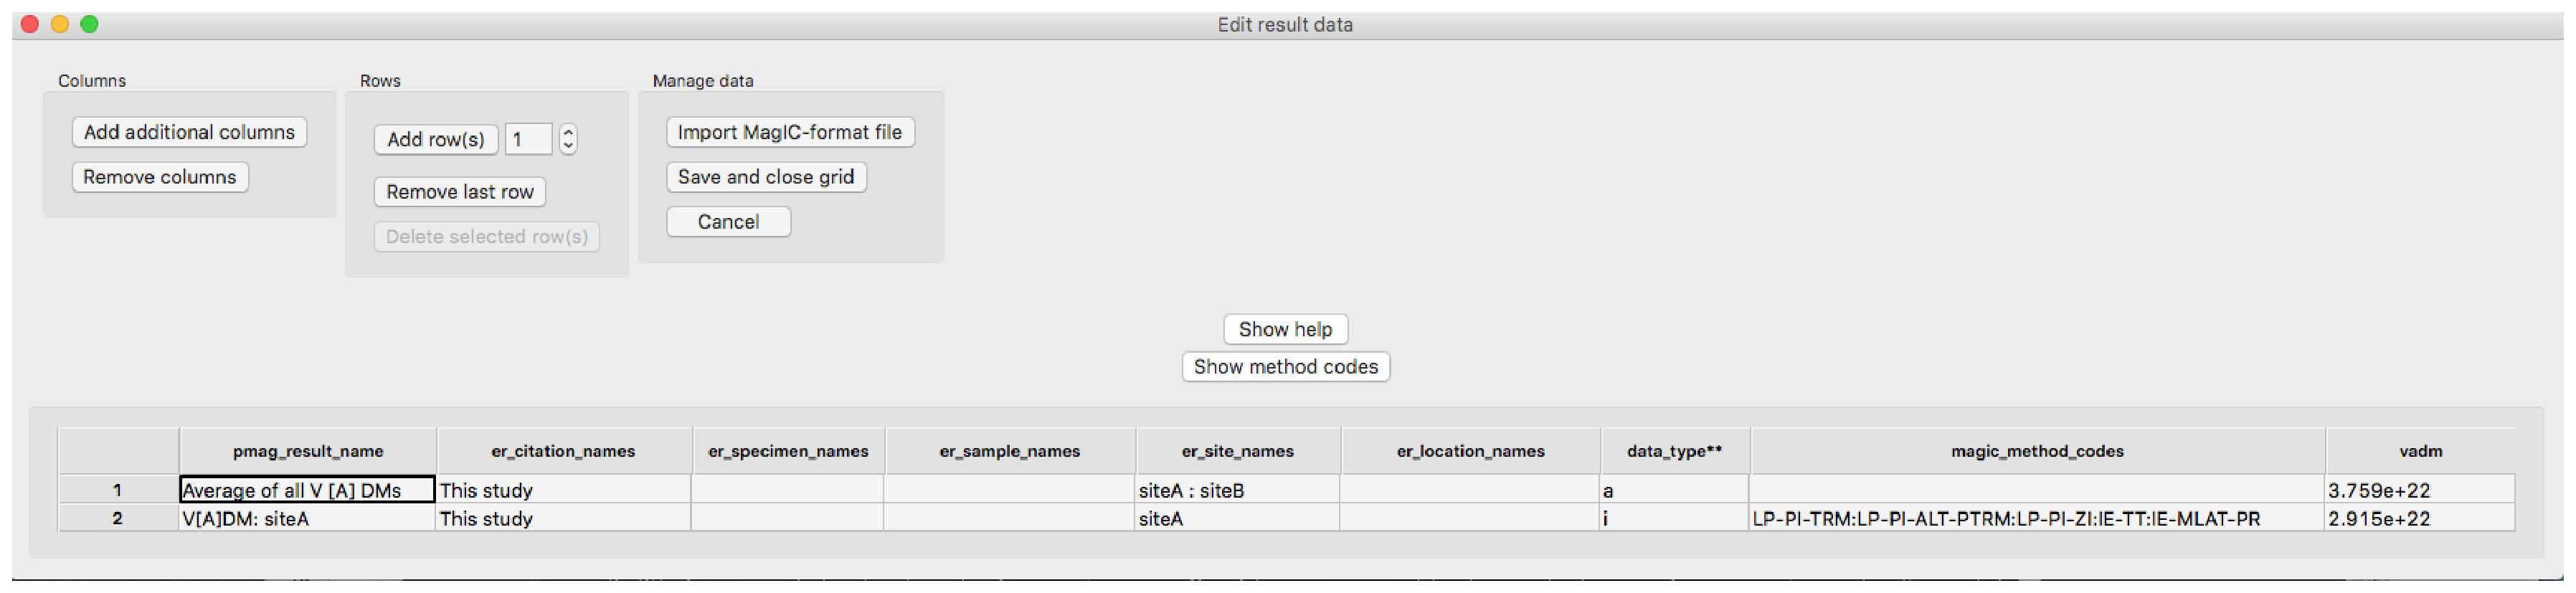
\includegraphics{EPSfiles/MM_result_grid.eps}

  \item For each result, you will add one or more items that the result pertains to.  In this example, one result is a site V[A]DM, and the other is an averaged V[A]DM from both sites.  For now, leave magic\_method\_codes blank for the Averaged V[A]DM result: in a minute we'll see how MagIC GUI catches this error.  Save and close the result grid.

  \item Next, you will create a MagIC format upload file.  Click the final button on the main frame, `prepare upload txt file'.  Depending on the size of your contribution, this can take a minute; with our small example, it should be fairly quick.  After hitting upload, you will see an error message, and the main frame will direct you to the problem.  Validations will check for missing required fields, invalid data, and missing ancestors (for instance, a specimen with no sample). 

    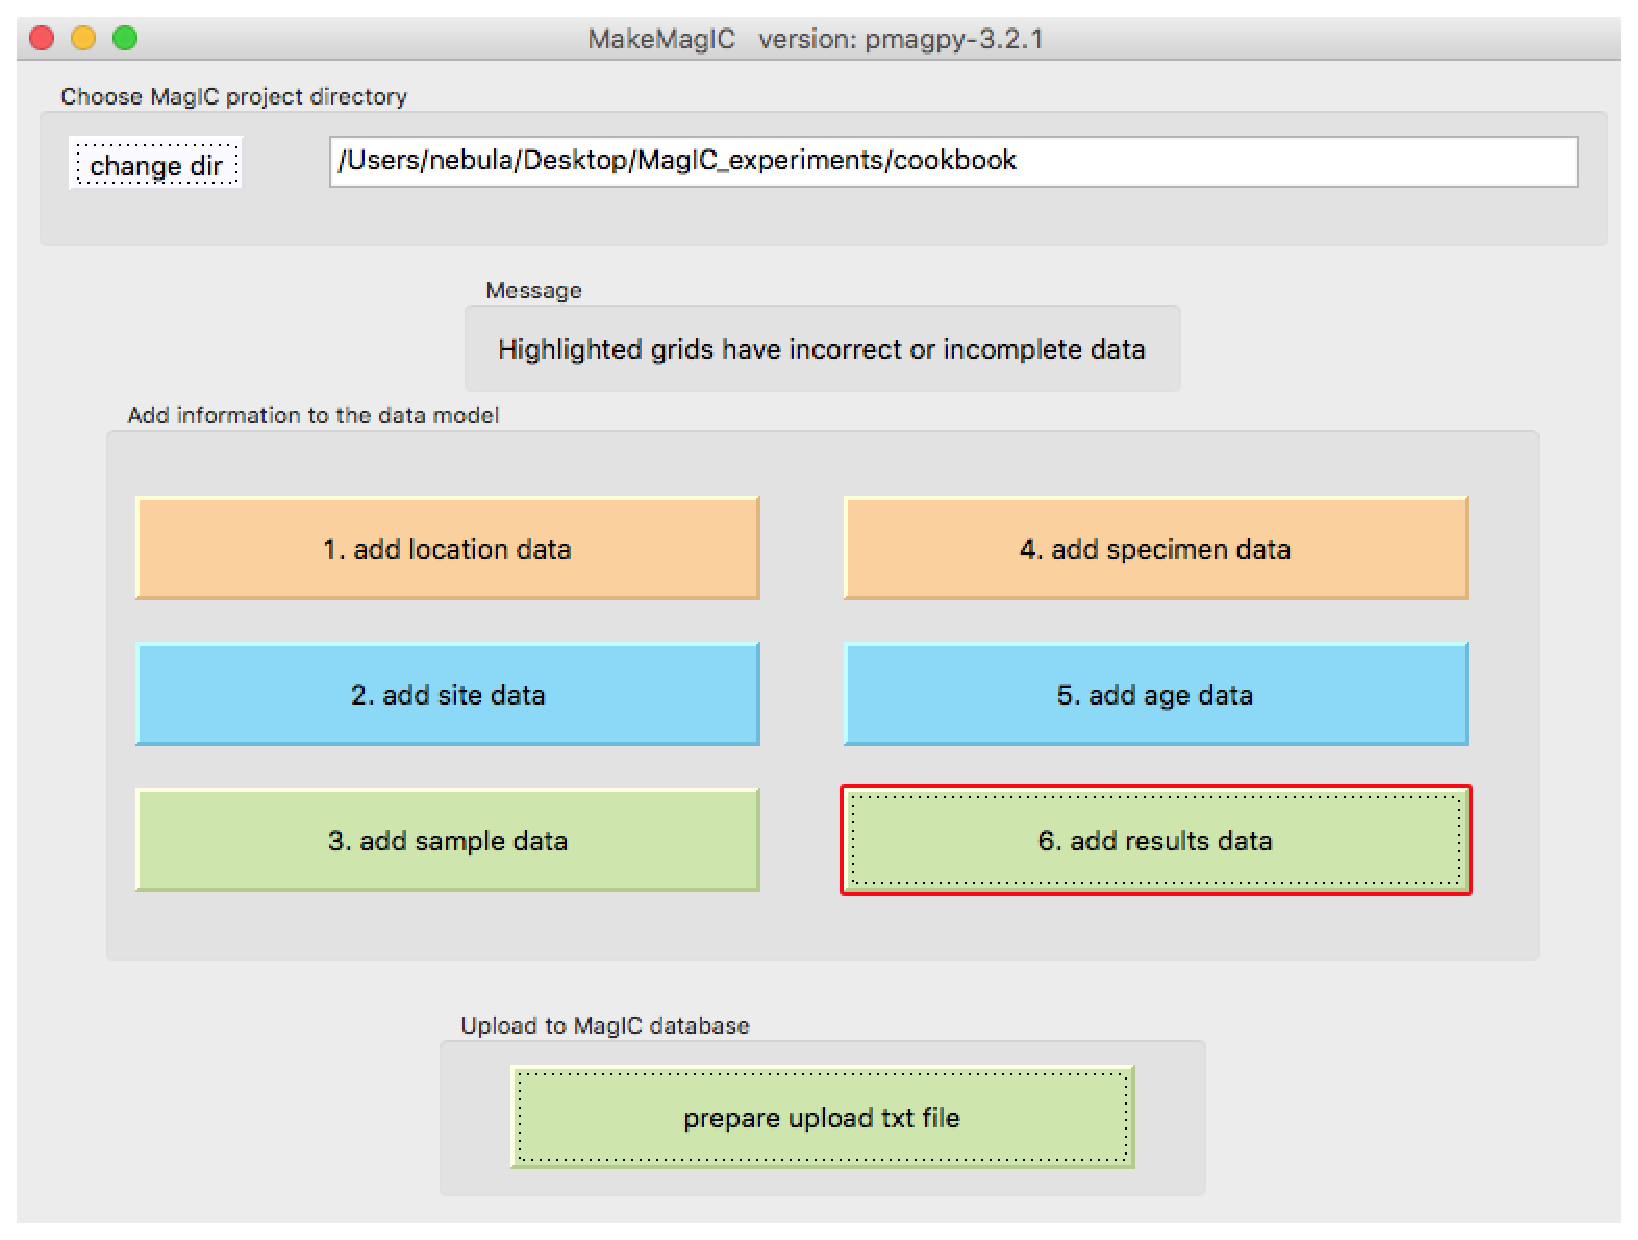
\includegraphics{EPSfiles/MM_validation_mainframe.eps}

    Open the result grid to fix the error.  Click `Show help' for more information about validations.  In this case, it is a simple fix: add method code `LP-PI' to the average V[A]DM result.

    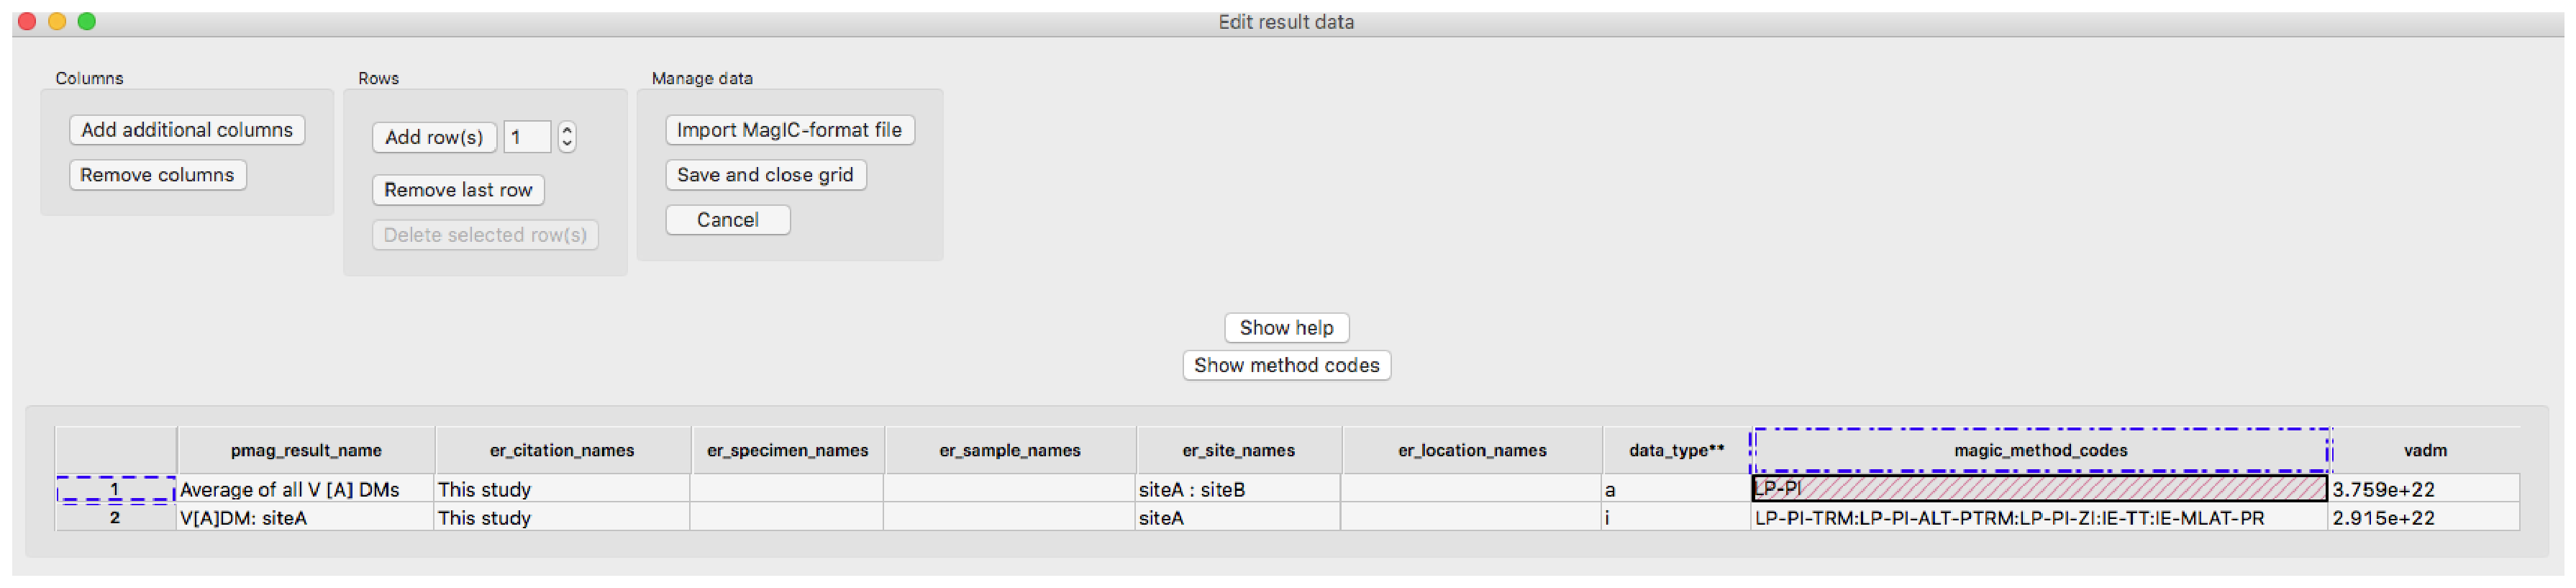
\includegraphics{EPSfiles/MM_filled_in_result_validation.eps}

  \item Now that you've fixed your error, try `prepare upload txt file' again.  This time there should be no problems, and you are ready to \href{#magic_upload}{upload your data}!

\end{itemize}
  



%
%
%\customlink{MagIC.py}
%
%\chapter{MagIC.py}
%\label{chap:MagIC} \href{#MagICDatabase}{[MagIC}]
%
%While \href{#pmag_gui.py}{Pmag GUI} provides a bare bones interface for importing, interpreting and uploading most demagnetization and paleointensity experimental data into the MagIC database, {\bf MagIC.py} is a more complete (and complicated) program.
%It is an umbrella program that links many MagIC related functions of the \href{#PmagPy}{PmagPy} Software Package in a user-friendly  graphical user interface (GUI).  While it is invoked with a command line call, this  can be done from any directory (with no spaces in the path).  It generates calls to the programs described in Chapter~\ref{chap:PmagPy} so you don't have to.    It allows importing of many lab and instrument formats, plotting of a variety of data and doing the data processing and book-keeping required to create files ready for uploading into the MagIC Console software.




\customlink{survival_skills}

\chapter{Survival computer skills}
\label{ex:unix}

The `Py' part of  `PmagPy' stands for Python, the language in which all the code is written.   It is not essential, but it is helpful to understand a bit about computer operating systems and the Python language when using PmagPy because no one should be using programs as black boxes without understanding what they are doing. As all the programs are open source, you have the opportunity to look into them.  If you understand a bit  about how computers work yourself, you will be able to follow along what they are doing and even modify them to work better for you.   So in this chapter you will find a brief introduction to the computer skills necessary for using the programs properly.  We have tried very hard to make this tutorial operating system independent.  All the examples should work equally well on Mac OS, Windows and Unix-type operating systems.  For a more complete explanation of the marvelous world of UNIX, refer to the website at \url{http://www.tutorialspoint.com/unix/unix-quick-guide.htm}.  For handy tricks in DOS, try this link:  \url{http://www.c3scripts.com/tutorials/msdos}.
For an introduction to programming in Python, see the  Chapter on \href{#Python}{Python Programming}.   For now, we're just interested in getting started with \href{#PmagPy}{PmagPy}.


\customlink{command_line}
\section{Finding your command line}
If you are not using a Unix-like computer (*NIX), you may never have encountered a command line. While the \href{#pmag_gui.py}{Pmag GUI} is an attempt to make life as easy for you by constructing commands for you, you still need to find the command line to start it up.  Under the MacOS X operating system look for the Terminal application in the Utilities folder within the Applications folder. When it is launched, you will get a terminal window as shown below.  The Unix (and Mac OS) Bash shell has a \$ sign as a prompt.  I (LT) use the antiquated `C-shell'  (don't ask) with a \% for a prompt and  will use the \% prompt in the examples here, but any of these command line prompts will work.

  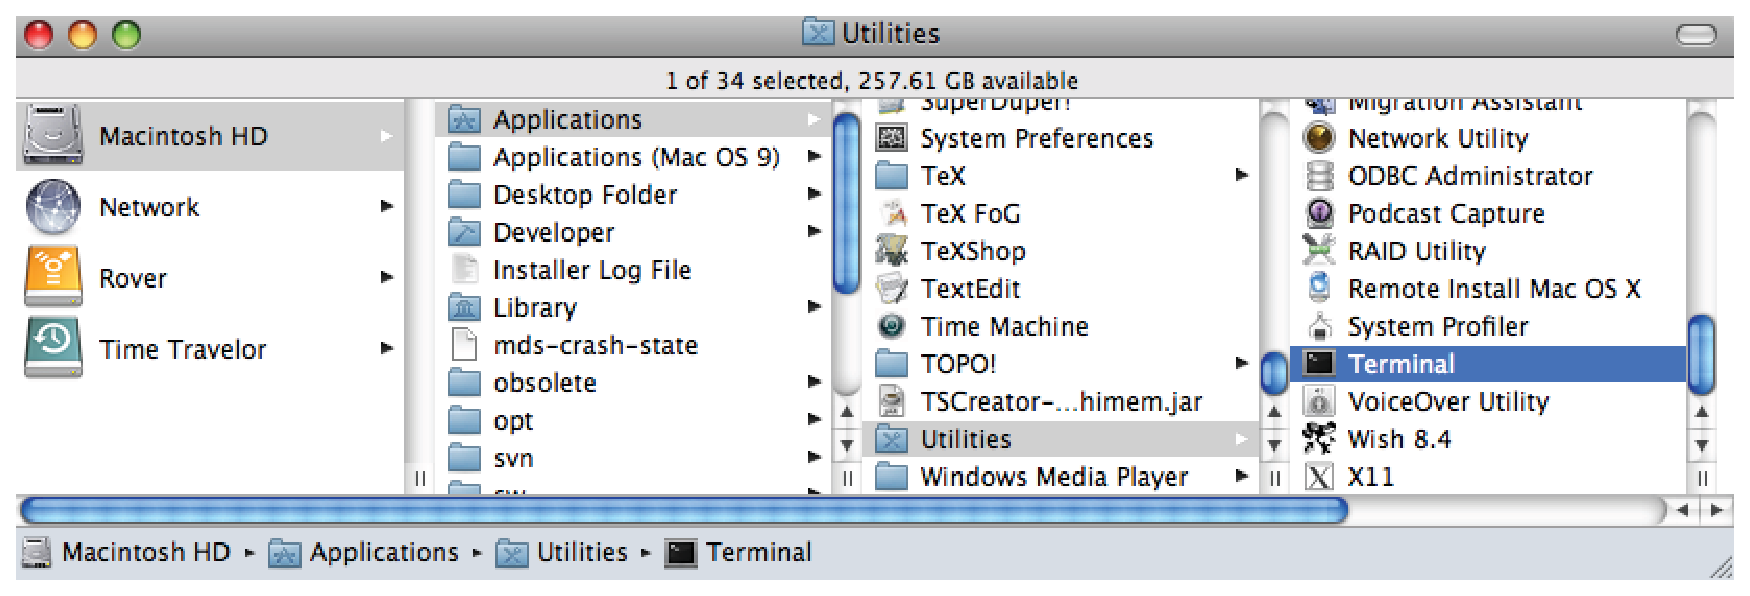
\includegraphics[width=15cm]{EPSfiles/terminal.eps}

Under the Windows operating system, if you followed the instructions in the  \href{#quick_start}{Installing PmagPy} section, you will have a shortcut to the PmagPy command window on your desktop.  Double clicking on that will give you a window in which you can type {\bf PmagPy} commands.

  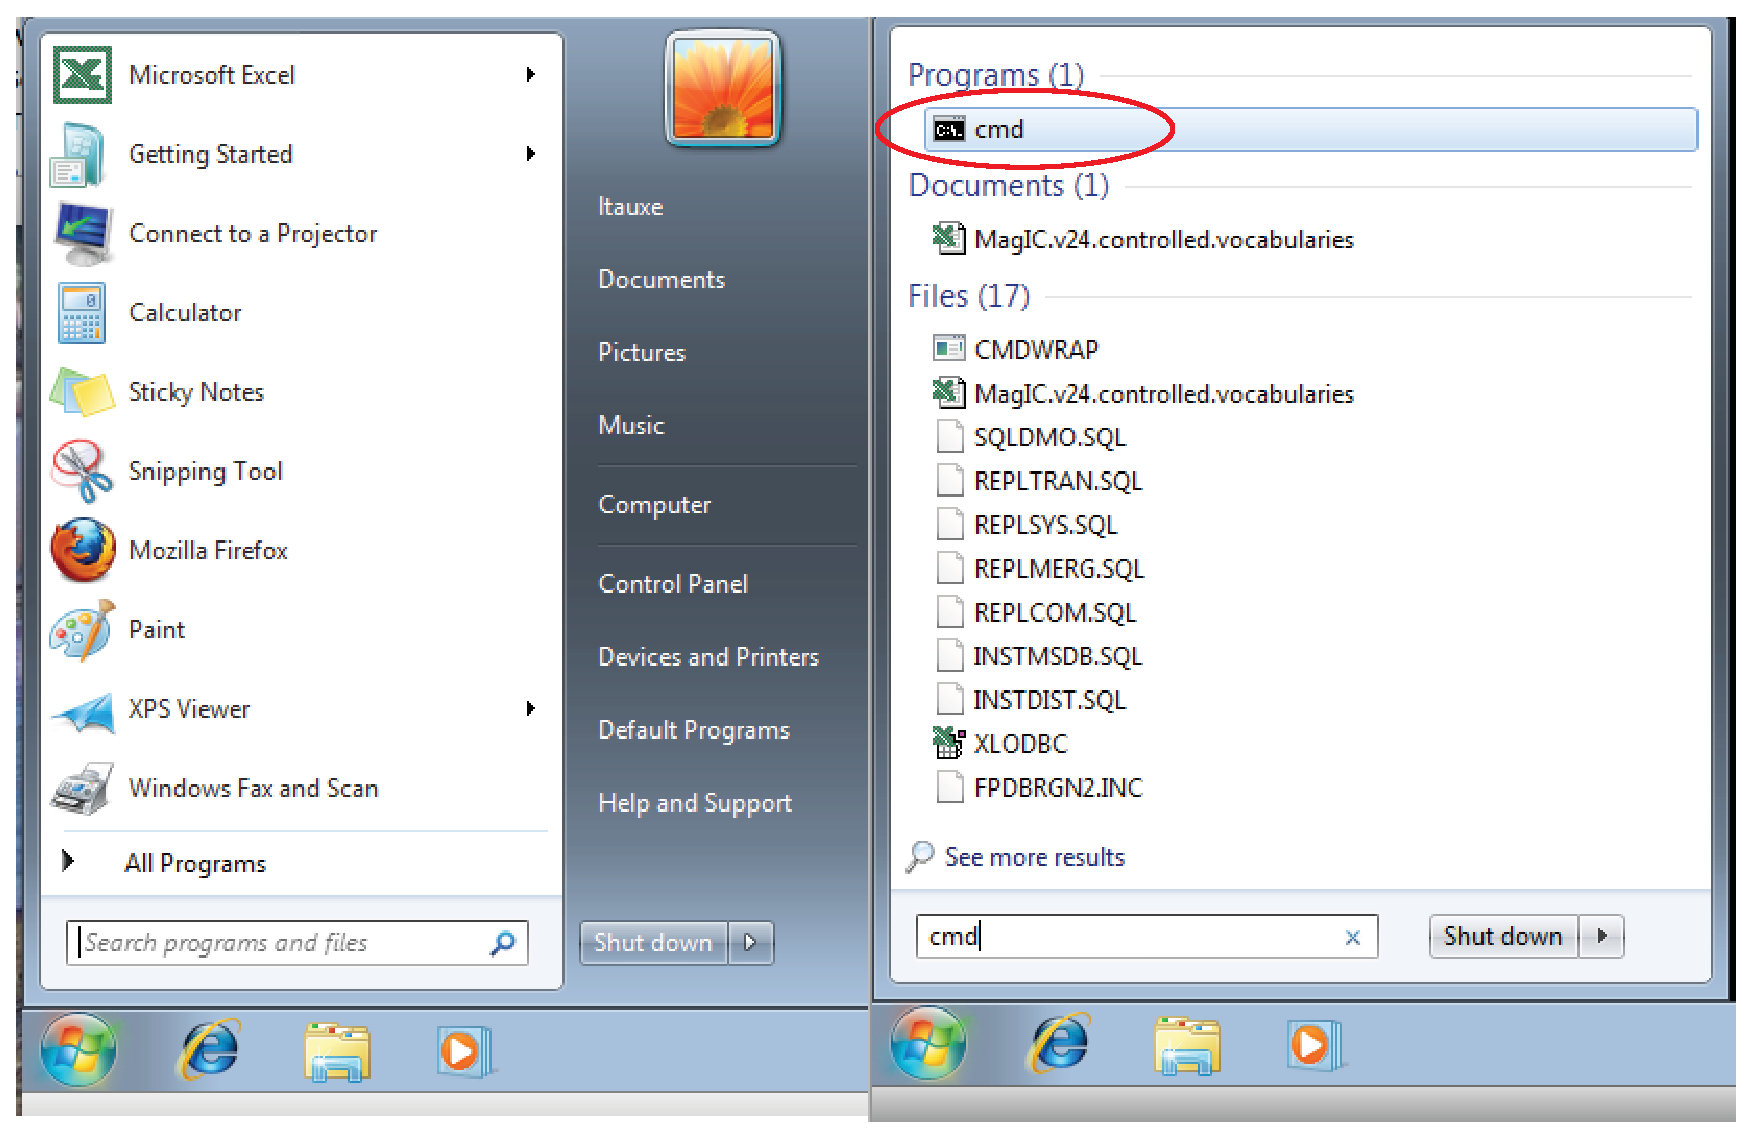
\includegraphics[width=15cm]{EPSfiles/cmd.eps}

  Note that the location of this program varies on different computers, so you may have to hunt around a little to find yours. Also, the actual  ``prompt'' will vary for different machines.



\section{File systems}
\label{sect:file_systems}
    When you open one of these terminal windows,  you are in your  ``home'' directory.
Fundamental to all  operating systems is the concept of
directories and files.  On windows-based operating systems (MacOS or Windows), directories are depicted
as ``folders'' and moving about is accomplished by clicking on the different icons.
In the world of terminal windows, the directories have names and are arranged in a hierarchical sequence with
the top directory being the ``root'' directory, known as  ``/'' (or C:'backslash' in Windows) and the file system looks something like this:


  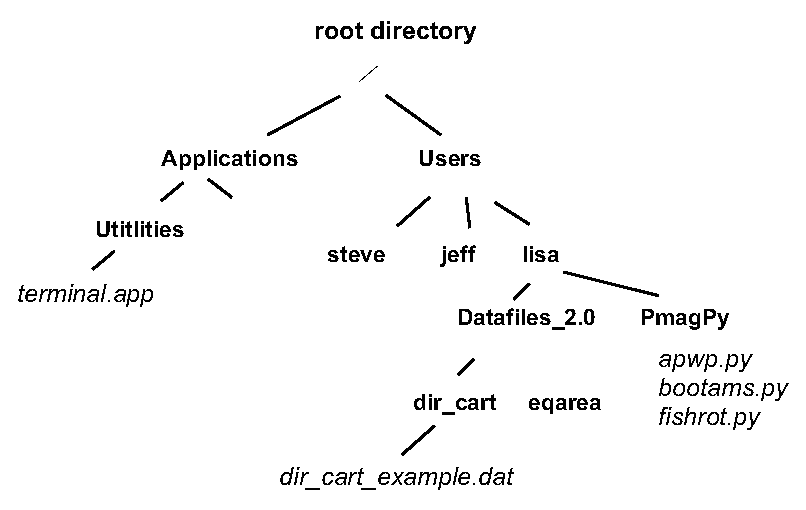
\includegraphics[width=15cm]{EPSfiles/filesys.eps}

 Within the root directory, there are subdirectories
(e.g. {\bf Applications} and {\bf Users} in bold face).  In any directory, there can also be ``files''
(e.g. {\it dir\_cart\_example.dat} in italics).   To
refer to directories,  the operating system relies on what is called a ``pathname''. Every object
has an ``absolute'' pathname which is valid from anywhere on the computer.  The
absolute pathname in *NIX always begins from the root directory {\bf /} and in DOS (the operating system working in the Windows command line window), it is C:'backslash'.

The absolute pathname to the home directory {\bf lisa} in the figure is {\bf /Users/lisa}.
Similarly, the absolute pathname to the directory containing {\bf PmagPy}
scripts  would be  {\bf /Users/lisa/PmagPy}.  There is also a ``relative'' pathname,
which is in reference to the  current directory (the one you are `sitting' in).  If user ``lisa'' is sitting in
her home directory, the relative pathname for the file {\it dir\_cart\_example.dat} in the directory
{\bf Datafiles\_2.0} would be {\it Datafiles\_2.0/dir\_cart/dir\_cart\_example.dat}.  When using relative
pathnames, it is useful to remember that {\bf ./} refers to the current
directory and {\bf ../} refers to the directory  ``above''.     Also, lisa's home directory would be $\sim$lisa, or if you are logged in as lisa yourself, then it is just $\sim$.



\section{Moving around in the file system}

Now that you have found your command line and are comfortable in your home directory, you can view the contents of your directory with the Unix command {\bf ls} or the DOS command {\bf dir}.
\customlink{mkdir}
You can make a new directory with the command
\begin{verbatim}
%mkdir NEW_DIRECTORY_NAME
\end{verbatim}
This works in both Unix and DOS environments) and you can move into your new directory with the command
\begin{verbatim}
% cd NEW_DIRECTORY_NAME
\end{verbatim}
   To move back up into the home directory, just type {\bf cd ..} remembering that .. refers to the directory above.  Also, {\bf cd} by itself will transport you home from where ever you are (there's no place like home....).     You can also change to any arbitrary directory by specifying the full path of the destination directory.


%\section {Wildcards}
%
%Unix and DOS have the ability to refer to a number of files and/or directories using
%``wildcards''.  The  wildcard for a  single character is ``?'' and for any number of
%characters is ``*''.  For example, to refer to all the files with ``.py'' in their name in the PmagPy directory in my home directory,
%I would type:
%
%\begin{verbatim}
%% ls PmagPy/*.py
%apwp.py bootams.py fishrot.py.....
%\end{verbatim}

\customlink{standard_IO}

\section {Redirecting input and output}

Programs that operate at the command line level print  output to the screen and read input
from the keyboard. This is
known as ``standard input and output'' or ``standard I/O''.
One of the nicest things about working at the command line level is the ability to redirect input and output.
For example, instead of typing input to a program with the keyboard, it can
be read from a file using the symbol {\bf $<$}.   Output can either be printed to the screen (standard output), redirected into a file using the symbol {\bf $>$}, appended to the end of a file with {\bf $>>$} or
used as input to another program with the pipe operator ({\bf$ |$}).



\section{Text editors}

There are many ways of
editing text and the subject is beyond the scope of this documentation. Text editing is a blessing and a curse.  You either love it or
hate it and in the beginning, and if you are used to programs like Word, you will certainly hate it. (And if you are used to a decent text editor, you will hate Word!).      But you can't use Word because the output is in a weird format that no scripting languages read easily.  So you have to use an editor that will produce a plain (ascii) file, like Notepad,  TextWrangler or Sublime Text.  \href{http://textwrangler.onfreedownload.com}{TextWrangler}  is freeware available for Macs and the notepad comes standard in the Windows operating system.   Fortunately for Mac users, Enthought Python's Canopy programming environment comes with its own text editor.

\customlink{PmagPy}

\chapter{The {\bf PmagPy} software package}
\label{chap:PmagPy}

The {\bf PmagPy} software package is a comprehensive set of programs for paleomagnetists and rock magnetists.  For installation,  follow the instructions in the \href{#quick_start}{Installing PmagPy} Chapter in this cookbook.

When you type something on your \href{#command_line}{command line}, your operating system looks for programs of the same name in special places.  These are special ``paths'' so the directory with your Python scripts has to ``be in your path''.  To inform the operating system of the new directory, you need to ``set your path''.    It should have been set when you installed {\bf PmagPy}.

\section{Graphical data analysis programs}
\subsection{demag\_gui.py}

The demag\_gui program enables the display and analysis of paleomagnetic demagnetization data. The software will display specimen level data within the chosen directory as a Zijderveld plot, equal area plot and intensity plot. Interpretations can be made to the data as least-squares line or plane fits. These interpretations can then be exported as MagIC pmag files.

\subsubsection{Launching}\label{launching}

The best way to launch the Demag GUI application is through the
Pmag GUI app. If PmagPy has been added to your PATH you can type pmag\_gui.py at the command line to launch it or you can navigate to the directory containing it and type \texttt{python  ./pmag_gui.py}. Within the Pmag GUI app, data can be converted from the format of a particular lab into MagIC format so that it can be displayed and analyzed within the demag\_gui. The program can be started by clicking on the demag\_gui button in the Pmag GUI, shown below. If no new window pops up after clicking this button, click on the Python icon  (the little space ship) on your dock.

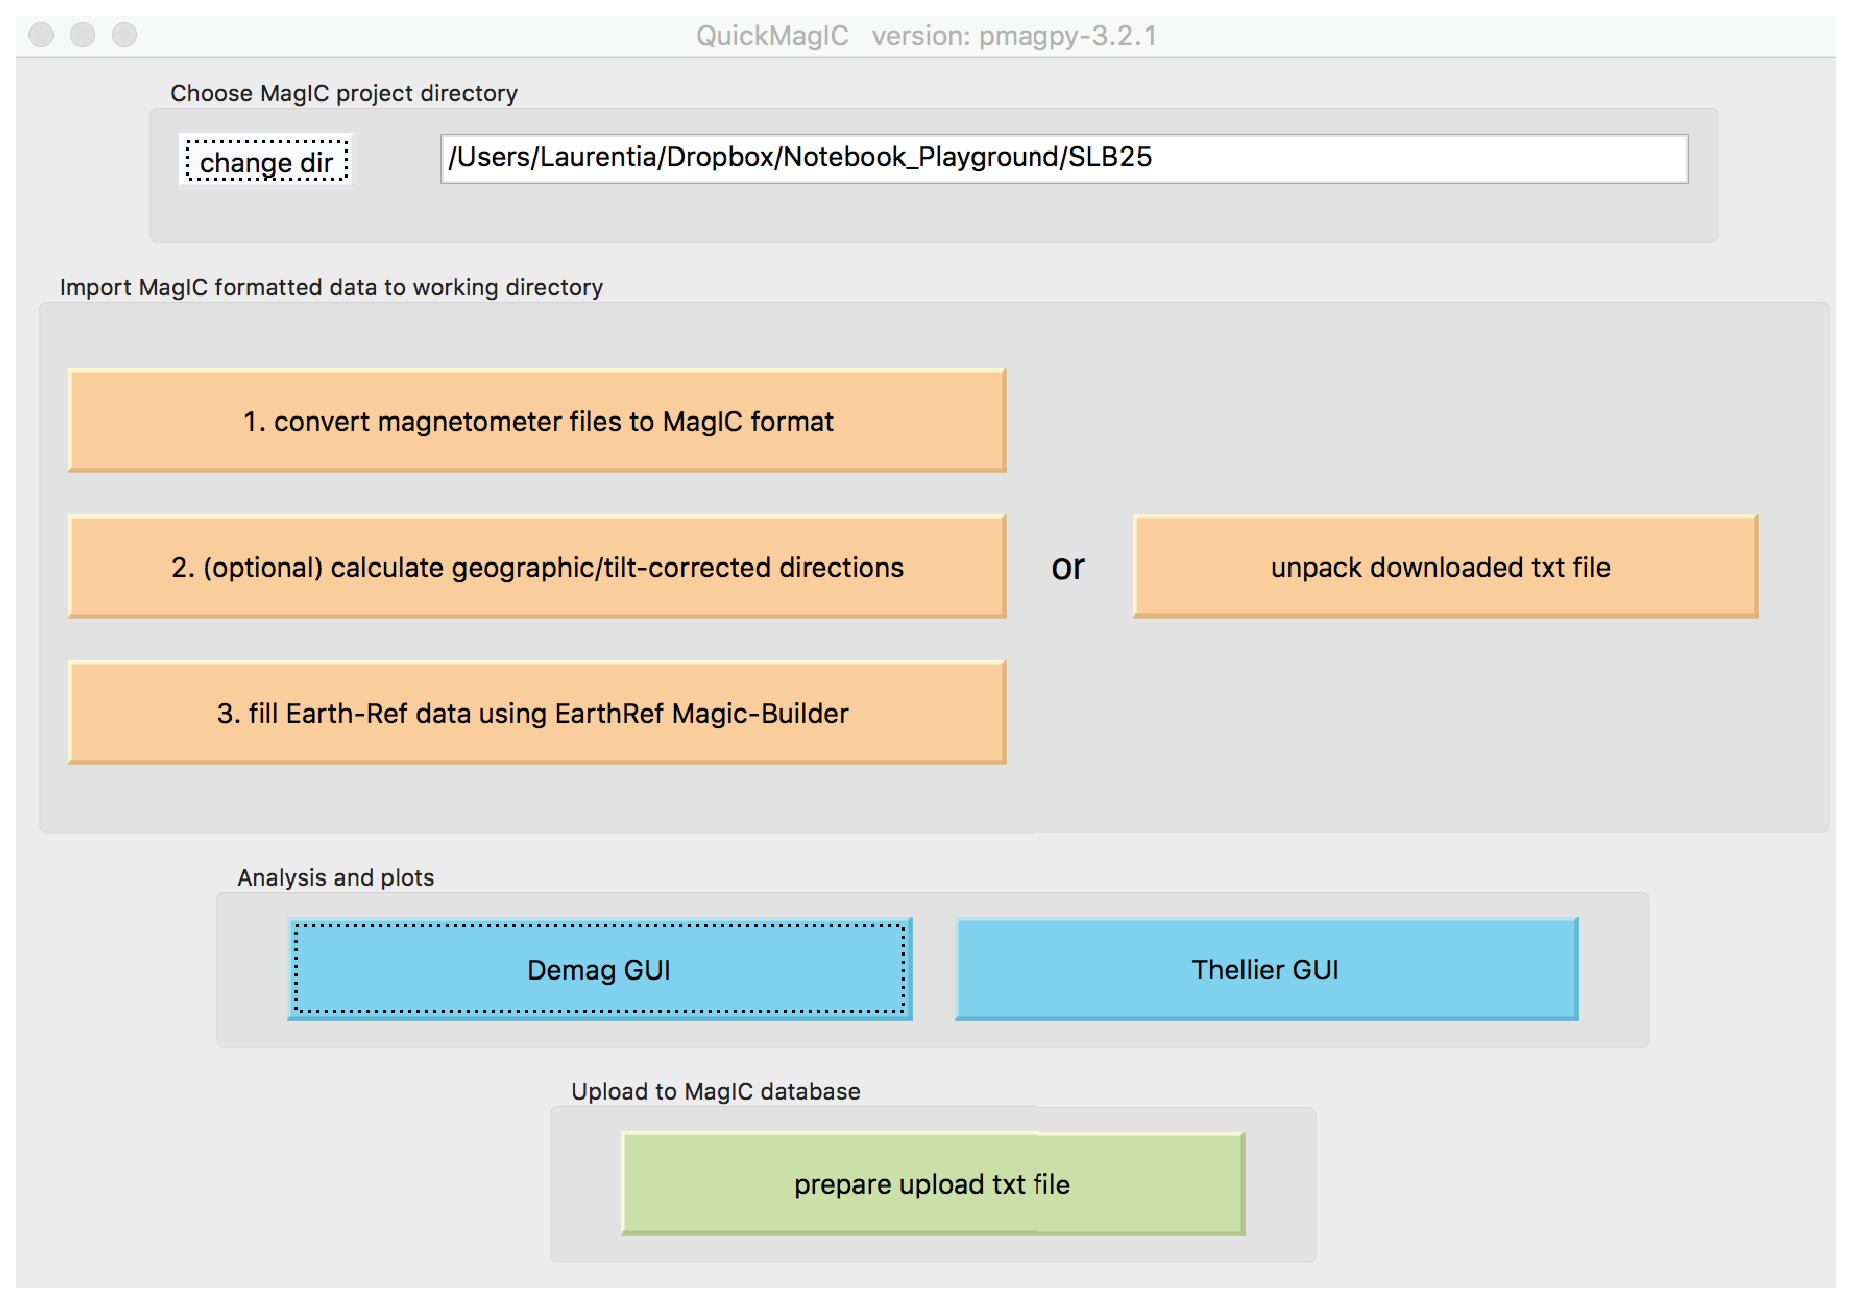
\includegraphics[width=10 cm]{EPSfiles/demag_gui_QuickMagicLauncher.eps}

Alternatively, Demag GUI may be launched through the command line by navigating to the directory containing demag\_gui.py and running it with: \texttt{python ./demag\_gui.py}.

Or if PmagPy has been added to your PATH you can simply type
demag\_gui.py at the command line. \textbf{Note:} on OSX it is
recommended to launch through Pmag GUI as on wxpython 2.9 the drop down boxes behave better when demag\_gui is launched this way.

\subsubsection{Adding Interpretations:}\label{adding-interpretations}

A least-squares fit to the measurement data can be added by clicking the add fit button. Additionally, you can select the fit you would like to edit or view by using the drop down box under the add fit button. Once you have selected a fit, the shape of the end points of the selected fit will turn to a diamond shape to distinguish them from the other data points.\\
\includegraphics[width=10 cm]{EPSfiles/demag_gui_Fit.eps}

Once the desired fit is selected, its bounds can be edited using the drop-down boxes under the bounds header.

\includegraphics[width=3 cm]{EPSfiles/demag_gui_BoundsBox.eps}

Alternatively, one can double-click the list of measurement steps on the left to pick out the bounds for the interpretation. The included steps in the currently selected interpretation are shown in highlighted in blue on the measurement list and the measurements marked ``bad'' are shown in yellow. \textbf{Note:} in case of duplicate measurements the first \emph{good} measurement with the same treatment is used.\\
\includegraphics[width=5 cm]{EPSfiles/demag_gui_DataBox.eps}

When first created, the fit will be given a generic name such as
\emph{Fit 1}. The name of the fit can be changed from the default by typing into the drop down box containing fit name then pressing enter. The default fit type is a least-squares line. You can choose different fits such as a line anchored to the origin or a plane by using the drop-down menu under specimen mean type. Planes can be plotted as either poles, full planes or partial planes. This display option can be changed in the second drop-down menu under specimen mean type.

\includegraphics[width=10 cm]{EPSfiles/demag_gui_SpecimenMeanType.eps}

The choice between coordinate systems (i.e.~specimen, geographic or tilt-corrected) is available on the left above the list of steps. The orientation of the Zijderveld projection can also be changed here.

\includegraphics[width=5 cm]{EPSfiles/demag_gui_ProjectionChoice.eps}

The properties of the currently selected fit to the data can be seen in the upper center of the GUI in a box labeled specimen mean statistics.

\includegraphics[width=15 cm]{EPSfiles/demag_gui_FitData.eps}

\subsubsection{Flagging Bad Measurement
Data}\label{flagging-bad-measurement-data}

Due to flux jumps or other such errors, individual measurements should sometime be excluded from interpretation. Such a measurements can be flagged as ``bad'' by right-clicking them within the measurement list and the measurement will then be highlighted in yellow. The measurement\_flag in the magic\_measurements file will be change from ``g'' to ``b'' when a measurement is marked as ``bad'' and the step will not be included in fits that are made to the data. Any measurement marked as `bad' will be colored yellow in the step list and will be shown as an empty rather than filled circle on the Zijderveld, equal area and M/M\_0 plots. To change a `bad' measurement back to being `good' one can right click on it again. Upon doing so, the yellow highlighting will go away, the data will be shown colored in within the plots and any fit that spans that data point will be recalculated to include it.

Acceptance criteria can be set by using Analysis/``Acceptance
Criteria''/``Change Acceptance Criteria''. These criteria will be written to a pmag\_criteria table.

\subsubsection{Plot Interface}\label{plot-interface}

The 4 plots that take up the majority of the center of the GUI are where data and their interpretations are displayed. The Zijderveld and the 2 equal area plots are by default set to zoom when you left click and drag your left mouse button you will zoom to the dragged out rectangle(currently equal area plots do not draw this rectangle as you drag your mouse, but still zoom). On the Zijderveld plot, it is possible to switch between zoom and pan functionality by right clicking. Once in pan mode, the mouse will turn into a hand allowing you then to click and move around the plot. On both the Zijderveld and equal area plots if you wish to return to the original plot simply click the middle mouse button to return to home position. \textbf{Note:} in the absence of a middle mouse button pressing both right and left mouse buttons at the same time works on most laptops in the case of Macbooks clicking with two fingers should work, and if using Apple's magic mouse we recommend you download the \href{http://magicprefs.com/}{MagicPrefs} program which will allow you to configure your mouse however you prefer. One the equal area plots you can double click on an interpretation to switch the specimen and current interpretation to the clicked interpretation.

\subsubsection{Saving Specimen
Interpretations}\label{saving-specimen-interpretations}

Once you have picked out your interpretations, you can save the session data in two different ways: (1) as a .redo file which will allow you to have the fits preserved to be view again with demag\_gui or (2) as MagIC pmag tables to be uploaded to the MagIC database or otherwise processed. In addition, you may save image files of the plots.

\paragraph{The .redo File:}\label{the-.redo-file}

You can use Analysis/``Save current interpretations to a redo file'' to create this file type or you can just hit the save button next to add fit. \textbf{Note:} this file type does \textbf{NOT} load previous interpretations on start up you must go to the menu option Analysis/``Import previous interpretations from a redo file'' to restore your previous session.

\paragraph{The Pmag Tables:}\label{the-pmag-tables}

By going to the menu File/``Save MagIC pmag tables'' you can export your interpretations made in Demag GUI to the MagIC pmag tables which can then be used by other MagIC programs or uploaded to the MagIC database. You can export any or all of the 3 coordinate systems upon selecting this option and you may choose to save pmag\_samples, pmag\_sites, and pmag\_results tables in addition to the pmag\_specimens table that is output. If you choose to output additional information you will be prompted by a pop up window for additional information. \textbf{Note:} this save format loads on start up of the GUI immediately restoring your session. Selection of this option will overwrite your demag\_gui.redo file in the working directory.

\paragraph{Images of Plots:}\label{images-of-plots}

Select the menu option File/``Save plot''/``Save all plots'' to save all plots. Alternatively, you can save any of the plots individually. If you zoom on any of the plots the zoomed image will be saved not the originally plotted image although the plot will redraw and reset the zoom level.

\subsubsection{Deleting Specimen
Interpretations}\label{deleting-specimen-interpretations}

If you would like to delete a single interpretation, select the one you wish to delete from the interpretation drop down menu and click delete. Alternatively, if you wish to clear all interpretations you may go into the interpretation editor located under the tools menu, select the fits you wish to delete and click the ``delete selected'' button.\\

\subsubsection{Higher Level Plots and
Interpretation}\label{higher-level-plots-and-interpretation}

The set of drop down boxes to the right of the interpretation data are there to determine what level you want to analyze in the higher level analysis options include: site, sample, location, and study. The drop-down below this selects which of the available sites, samples, location, or studies to display.

You can then select how to group your data by using the drop down menu under the show header. You can select what kind of mean to take using the first drop down under the mean header. Which interpretations to use for the means can be selected under the second drop down menu.

The mean statistics for the chosen higher level mean are displayed in the lower right of the GUI.

\subsubsection{Interpretation Editor}\label{interpretation-editor}

In order to more easily view and edit specimen interpretation data there is a specimen interpretation editor which can be launched from the tools menu. This panel details the fits made to the data and their parameters from which you can select which interpretation to view by double clicking on it. In the list, the currently selected interpretation is highlighted blue as shown in the image below. You can mark interpretations as bad which removes them from any Fisher means or other high level means by right clicking on their entry in the list. All interpretations marked bad are colored yellow in the list and marked as an `x' on the plot. The specimen entry associated with this fit will be given a bad (`b') flag within the pmag\_specimens table. Interpretations can be highlighted by clicking on the list and holding the shift or ctrl/command key to select multiple interpretations. Doing so allows you to delete or alter the characteristics of multiple interpretations at once without having to select each one in turn. This mass alteration is allowable using the the Name/Color/Bounds boxes to input the changes and then clicking the ``apply changes to highlighted fits'' button. You can delete highlighted fits using the ``delete highlighted fits'' button. The ``add fit'' button in the interpretation editor adds a fit to the current specimen. In the case of interpreting large data sets, you can reduce the number of items plotted on the equal area at the bottom of the editor and the number of entries in the log by changing the display settings.

\includegraphics[width=15 cm]{EPSfiles/demag_gui_InterpEditor.eps}

\customlink{thellier_GUI.py}

\subsection{thellier\_gui.py}
\href{http://earthref.org/MAGIC/books/Tauxe/Essentials/WebBook3ch10.html#ch10}{[Essentials Chapter 10]} and \href{#MagIC}{[MagIC}]
\href{https://github.com/ltauxe/PmagPy/blob/master/Thellier_GUI_tutorial.pdf}{[Thellier\_GUI\_tutorial.pdf]}

The program {\bf thellier\_gui.py}  combines functions from \href{#thellier_magic.py}{thellier\_magic.py} and new tools described by  \href{http://dx.doi.org/10.1002/ggge.20062}{Shaar and Tauxe (2013)} \nocite{shaar13} in a user-friendly graphical user interface (GUI).  It can also be called from within \href{#pmag_gui.py}{Pmag GUI}, using files already prepared in a  \href{#ThisProject}{This Project} directory and the interpretations from {\bf thellier\_gui.py} are part of the workflow of  \href{#pmag_gui.py}{Pmag GUI}.   This section is a brief introduction on how to use {\bf thellier\_gui.py} as a stand alone application.

\noindent  A complete list of the definitions for paleointensity statistics used by Thellier\_GUI.py is available as a supplement to the article by \href{#http://dx.doi.org/10.1002/2013GC005135}{Paterson et al., 2014}  \nocite{paterson14} and available for download here:

  \url{http://onlinelibrary.wiley.com/store/10.1002/2013GC005135/asset/supinfo/ggge20412-sup-0001-suppinfoCORRECTED.pdf?v=1&s=e1c3ab0a86c942d1039f6d2e15496aa172dc86ec}


\subsubsection{Starting the GUI}
The GUI can be opened by typing {\bf thellier\_gui.py}  on the  \href{#command_line}{command line}.

\customlink{choose_directory}
A ``choose project directory'' dialog window will appear as soon as the GUI is started.
%
%	\includegraphics[width=15cm]{EPSFiles/Screenshot_choose_directory.eps}
%
%
Your  \href{#Project_Directory}{ThisProject} directory should include a file named {\it magic\_measurements.txt} (created for example by \href{#pmag_gui.py}{\bf Pmag GUI}.   If a file named {\it rmag\_anisotropy.txt} is in the project directory, then the program reads in the anisotropy data. Reading and processing the measurements files may take several seconds, depending on the number of the specimens.


\subsubsection{Reading and compiling measurements data}
When your \href{#Project_Directory}{ThisProject}  project directory is selected, the program  reads all the measurement data, checks them, processes them and sorts them. If non-linear-TRM (NLT) data exist in {\it magic\_measurement.txt}  then the program tries to process the data using Equations (1)-(3) in \href{#http://dx.doi.org/MAGIC/doi/10.1016/j.epsl.2009.12.022}{Shaar et al., 2010}. \nocite{shaar10}  The program reads {\it magic\_measurement.txt}, and processes the measurements for presentation as Arai  and Zijderveld plots.
We recommend that you check all the warnings and errors in {\it Thellier\_GUI.log} before starting to interpret the data.  For details about warnings and error messages during these steps, consult the tutorial document in the {\it thellier\_GUI} folder in  \href{#Datafiles}{Datafiles}.  Also, consult the Preferences to change certain plotting options.

\subsubsection{Main panel}

This figure shows a snapshot of the main panel.

	\includegraphics[width=30cm]{EPSFiles/Screenshot_main_panel.eps}

\noindent
	The top field in the  panel includes the following buttons/controls (from left to right):
	\begin{itemize}
\item {\bf Specimen:} a list of the specimens in the project folder sorted by name.
\item {\bf previous/next:} buttons to move forward and backward in the specimens list.
\item {\bf T min/T max:} buttons to select temperature bounds.
\item {\bf save/delete:} save or delete current interpretation. This information will be used later to generate a \href{#mk_redo.py}{redo file}.
\item {\bf B\_lab:} laboratory field in units of $\mu T$.
\item {\bf B\_anc:} specimen's paleointensity in units of $\mu T$.
\item {\bf Aniso Correction:} anisotropy correction factor.
\item {\bf NLT Correction:} Non-Linear TRM (NLT) correction factor.
\item {\bf Dec/Inc:} Specimen declination/inclination calculated by PCA of the NRM in the selected temperature bounds.
\item Sample mean, number of specimens, standard deviation and percent standard deviation.
\end{itemize}

The center of the main panel has these elements:

\begin{itemize}
\item {\bf measurements text panel:} Four columns of the measurement data: Step is ``N`` for NRM, ``Z`` for zero field step, ``I`` for infield step, ``P`` for pTRM check, and ``T`` for tail check. The temperature of each step is given in C. Also shown  declination, inclination and moment (in units of $Am^2$)
\item {\bf Arai plot:}  Arai plot normalized by $NRM_0$. blue circles are zero field steps, red circles are infield steps, triangles are pTRM checks, blue squares are tail checks. Temperatures are displayed near data points. Temperature bounds and best fit line are marked in green. 'SCAT box' is marked with dashed lines (only if SCAT is True).
\item {\bf Zijderveld plot:}  A Zijderveld plot of the NRM step.  The x axis is rotated to the direction of the NRM, blue is the x-y  projection, and red is x-z projection.
\item {\bf Equal area plot:}  An equal area projections  of the NRM steps. solid circles are positive inclination. open circles are negative inclinations.
\item {\bf Moment-temperature plot:}  NRMs are in blue, pTRMs are in red.
\item {\bf sample data:}  If at least two specimens have a saved interpretation, then their values are displayed on this plot. The mean $\pm$ standard deviation of the mean are marked as  horizontal lines.
\end{itemize}

The bottom of the main panel include paleointensity statistics. The first line has  the threshold values (empty if N/A). The second line is the specimen's statistics. For details see Appendix A1 in \href{http://dx.doi.org/10.1002/ggge.20062}{Shaar and Tauxe (2013)}. \nocite{shaar13}
%
%\subsubsection{ Tutorial by example}
% If you have not already done so, locate  the example data files for PmagPy in the \href{#Datafiles}{Datafiles} directory bundled with the {\bf PmagPy} software package.   There are two folders located in the{\it thellier\_gui} example foler: SU1\_example and Tauxe\_2006\_example.
%
%
%{Case study 1: SU1\_example:}
%
%Find your \href{#command_line}{ command line} and launch the program:
%\begin{verbatim}
%thellier_gui.py
%\end{verbatim}
%A \href{#choose_directory} {choose directory} dialog window will appear. Select the SU\_1 project directory and click on the ``choose'' button.
%
%\begin{itemize}
%\item{Manual interpretation}
%Manual interpretation is the conventional approach of selecting temperature bounds for each specimen. Here, as example, we will interpret one sample, su100601,  manually.
%%\customlink{acceptance_criteria}
%
%\begin{itemize}
%\item Set acceptance criteria: From the menu-bar choose  Analysis $\rightarrow$ Acceptance criteria $\rightarrow$ Change acceptance criteria. A criteria dialog box will appear.
%\item In the first line (specimen's statistics) set the following values: n=3, int\_ptrm\_n=2, SCAT=false (unchecked), gap\_max=0.5, f\_vds=0.75, beta=0.1, MAD=6, DRATS=20. delete the values in the other boxes (empty boxes).
%\item In the second line (Sample's acceptance criteria) set the following values: int\_n=3. delete the value in the other boxes.
%\item In the third line (Sample mean calculation method: STDEV-OPT) check the Enable/Disable box, and set the following values: int\_sigma=6, int\_sigma\_perc=10. Delete values in the other boxes. Figure 3 shows how it should look. Click on the OK button. A message dialog will appear telling you the criteria that you chose are saved in a file name pmag\_criteria.txt. The next time you will open the GUI in this project directory, these criteria will automatically be chosen. Click OK on the message box.
%\item Manual interpretation of sample su100601: choose specimens su100601a from the specimen list. choose temperature bounds from the Tmin/Tmax windows: 200 and 580. B\_anc shows 61.7 in green, which means that this interpretation passes the specimen's acceptance criteria. Now, change Tmax to 530.  B\_anc window change color to red, and also the fvds window (the row on the bottom of the GUI). This is an indication that the interpretation did not meet the criterion for fvds. Change  Tmax to 580 (as before) and press ``save`` button. The interpretation in saved.
%\item Click on the next button to choose the next specimen (su100601b). Before analyzing this specimen, press on the ``previous`` button, so you can see that your previous interpretation was saved. click on ``next`` to return again to specimen su100601b. Find  temperature bounds that pass the criteria (for example 200,580). Make sure that all colors are green, and click on the ``save`` button. Go over all the other specimens in the sample (su10060a to su100601g). you will find that three specimens can pass: a,c, and g. Look at the Sample data figure (top right) it shows the saved interpretation for all the specimens in the sample, and the mean $\pm$  standard deviation of the mean.
%\item To save all your interpretation into files, choose from the menubar Analysis $\rightarrow$ Save current interpretation. Three files will be generated in the project directory:
%\begin{itemize}
%\item thellier\_GUI.redo (the temperature bounds for each specimen):
%\begin{verbatim}
%su100601a 473 853
%su100601c 473 853
%su100601g 473 853
%\end{verbatim}
%Note that the temperature bounds are in Kelvin.
%\item {\it thellier\_GUI.specimens.txt}: (the paleointensity statistics for each specimen - according to the headers. It is easy to view the content of this file using Excel):
%\begin{verbatim}
%su100601a	su100601	61.7	200	580	40.0	1.07	1.01	15	8	0.77	0.87	0.89	0.14	0.02	N/A	0.63	N/A	5.11	4.14	PASS
%su100601c	su100601	54.4	200	580	40.0	0.94	N/A	15	8	0.60	0.78	0.79	0.23	0.01	N/A	5.19	N/A	2.51	1.33	PASS
%su100601g	su100601	58.4	200	580	40.0	1.00	1.01	15	8	0.70	0.83	0.85	0.19	0.02	N/A	2.80	N/A	3.12	1.96	PASS
%\end{verbatim}
%\item {\it thellier\_GUI.samples.txt:} (the paleointensity statistics of the samples):
%\end{itemize}
%\begin{tabular}{cccccc}
%\hline
%er\_sample\_name &sample\_int\_n&sample\_int\_uT&sample\_int\_sigma\_uT&sample\_int\_sigma\_perc\\
%su100601 &	3&	58.2&	3.0&	5.1\\
%\hline
%\end{tabular}
%
%
%\item You can save the Arai plot (or any other plots) from the File menu. Choose  file  $\rightarrow$ Save Plot $\rightarrow$ Save Arai plot. A file dialog window will appear. You can change the format of the figure in the bottom tab (pdf, svg, or png), but you can also save as other format by adding the appropriate suffix to the file name.
%\item close the GUI: File  $\rightarrow$ Quit.
%\item Re-open the GUI as before (by writing the command  ``thellier\_gui.py''  in the terminal window) and choose the same working directory (SU1\_example). Notice now that the criteria that you set before are automatically used. To import your previous interpretations and continue working on this dataset choose from the menu bar Analysis $\rightarrow$ import previous interpretation. Choose thellier\_GUI.redo and click on the 'open' button.
%\end{itemize}
%
%\item{Automatic interpretation - \it{thellier\_auto\_interpreter:}}
%Instead of trying to find manually the most appropriate temperature bounds, the  {\bf thellier\_auto\_interpreter.py} program allows a fast and consistent way to choose the temperature bounds for the specimens. For details see \href{http://magician.ucsd.edu/~ltauxe/CV/open/shaar12.pdf}{Shaar and Tauxe (2012)}.  \nocite{shaar12}
%\begin{itemize}
%\item We will use the same \href{#acceptance_criteria }{acceptance criteria}.
%\item Choose from the menu bar Auto interpreter $\rightarrow$ Run Thellier auto interpreter. The interpreter will run approximately 30 seconds. When its done, a message window will appear saying that the interpreter finished successfully (if not, check for errors in the terminal window, or in a file name {\it thellier\_interpreter.log}  located in a folder named {\it thellier\_interpreter}. If the issue cannot be resolved send an e-mail with the description of the problem to rshaar@ucsd.edu). Click OK in the message window.
%\item The automatic interpretations are automatically saved, and we can review them on the Arai plots.  Let's look, for example, at the sample we interpreted  manually: su100601. Choose specimen su100601a from the specimens list. At first glance, the choice seems strange because the automatic interpretation chose temperature bounds 0 and 580. A choice between 200 and 580 may seem more reasonable as it provides an nearly straight line. The sample data figure explains this issue. The {\bf thellier\_auto\_interpreter.py} program chooses the interpretations that minimize the standard deviation of the sample's mean. Six specimens from this sample passed the criteria, and the value of su100601a is much higher than the remaining five. So, the thellier\_auto\_interpreter chose the 'acceptable' interpretation with the shallowest  slope. Go over the other specimens in the sample, and review the automatic interpretations. If you want, you can change the automatic interpretation, and save your own ``manual'' interpretation by choosing Analysis $\rightarrow$ Save current interpretation. Note that the output of {\bf thellier\_auto\_interpreter.py} is sensitive to the choice of the acceptance criteria, and different criteria may lead to significantly different final results.
%\end{itemize}
%\item{Choosing the optimal criteria - \it{thellier\_optimizer\_2d:}}
%\href{http://magician.ucsd.edu/~ltauxe/CV/open/shaar12.pdf}{Shaar and Tauxe (2012)} \nocite{shaar12} discuss a method to choose the optimal specimen's acceptance criteria. Here, we follow the example given in this paper. \href{http://magician.ucsd.edu/~ltauxe/CV/open/shaar12.pdf}{Shaar and Tauxe (2012)} suggested using  seven statistics for specimen's acceptance criteria. The choice of four of which is trivial, and the remaining three are MAD, FRAC and $\beta$. The thellier\_optimizer\_2D helps finding the optimal values for FRAC and $\beta$.  The thellier\_optimizer\_2D  required three types of inputs: 'fixed\_criteria``, ``test\_groups``, and ``test\_samples``, as described below:
%\begin{itemize}
%\item The test groups are defined in an ``er\_sample`` file. An example for this file is given in working folder SU-1 named  ``optimizer\_test\_groups.txt``. Open this file in Excel to understand its syntax. The first line is a general header. The rest of the file include sample name, group name, and comments.
%\item To run the optimizer choose from the menu bar Optimizer $\rightarrow$ Run Thellier optimizer. click OK in the  message dialog. The first step is setting the 'fixed\_criteria``. We choose for the specimen's criteria: n=3, int\_ptrm\_n=2,SCAT=checked, gap\_max=0.6, MAD=5.0. We choose for the sample's criteria:int\_n=3, int\_n\_outlier\_check=6, EnableSTDEV-OPT, int\_sigme\_uT=5, int\_sigma\_perc=6. The rest of the boxes should be empty. click OK. click OK on the message window that will appear.
%\item The thellier\_optimizer\_2D dialog window will appear. The first two rows of controls for choosing the range for $\beta$ and FRAC. choose beta from 0.05 to 0.15 in steps of 0.1 and FRAC from 0.7 to 0.9 in step of 0.02. \\
%Inert the following functions to the text panel:\\
%study\_sample\_n\\
%max\_group\_int\_sigma\_uT\\
%((max\_group\_int\_sigma\_uT $<$= 5) or (max\_group\_int\_sigma\_perc $<$= 6)) and  int(study\_sample\_n) \\
%click on the ``Check function syntax`` button. If there are no typos, then the text box below the button should be PASS.\\
%click on the ``Choose optimizer group file`` button. A file dialog window will appear. choose the file ``optimizer\_test\_groups.txt``. Click the button ``Run Optimizer`` to start. The runtime using these parameter is about 8 minutes. `
%\item All the output files of the optimizer are saved in a folder named ``optimizer`` (see section 4.4). Compare the figures in the 'pdf' folder with Figure 7 in \href{http://magician.ucsd.edu/~ltauxe/CV/open/shaar12.pdf}{Shaar and Tauxe (2012)}.
%\item The figure in optimization\_function\_2.pdf suggest using $\beta \leq$0.10 and FRAC  $ \geq $0.79. Set these values as acceptance criteria, and run thellier\_auto\_interpreter.
%\end{itemize}
%\end{itemize}

\subsection{MagIC GUI}

This application provides a simple interface for transforming data from a paleomagnetic or rock magnetic study into the format necessary for contribution to the MagIC database.

\section{Command line PmagPy programs}

{\bf PmagPy}  scripts work by calling them on a \href{#command_line}{command line}.
 The python scripts must be placed in a directory that is in your ``path''.  To see if this has been properly done, type {\bf dir\_cart.py -h} on the command line and you should get a help message.  If you get a ``command not found'' message, you need to fix your path; check the ``installing python'' page on the software website.   Another possible cause for failure is that somehow, the python scripts are no longer executable.  To fix this, change directories into the directory with the scripts, and type the command:  chmod a+x *.py

For people who hate command line programs and prefer graphical user interfaces with menus, etc., some of the key programs for interpreting paleomagnetic and rock magnetic data are packaged together in a program called {\href{#pmag_gui.py}{Pmag GUI}.  This can be invoked by typing {\bf pmag_gui.py} on the command line.
The \href{#pmag_gui.py}{Pmag GUI} program generates the desired commands for you behind the scenes, so you do not have to learn UNIX or how to use the command line (except to call {\bf Pmag GUI} itself).  Nonetheless, some understanding of what is actually happening is helpful, because {\bf Pmag GUI} is more limited than  full range of {\bf PmagPy} programs.  So, here is a brief introduction to how the {\bf PmagPy} programs work.

All {\bf PmagPy} programs print a help message out if you type: {\bf program\_name.py -h} on the command line.  Many have an ``interactive'' option triggered by typing {\bf program\_name.py -i}.  Many also allow reading from \href{#standard_IO }{standard input and output}.   The help message will explain how each particular program functions.  There are some common features for the command line options:


\begin{itemize}
\item Switches are from one to three characters long, preceded by a '-'.
\item The switch '-h' always prints the help message and '-i' allows interactive entry of options.
\item  Options for command line switches immediately follow the switch.  For example:  -f INPUT -F OUTPUT will set the input file to INPUT and the output to OUTPUT.
\item  The switch for input  files all start with -f and -F for output files.
\item -spc -sam -sit -syn  -loc are switches relating to specimens, samples, sites, synthetics and locations respectively.
\item Capitalized switches suppress an option (e.g., -A means do not average, while -a means DO average).
\item -crd [s,g,t] sets the coordinate system
\item -fmt [svg,png,jpg] the default image format.
\item -sav  saves the plots silently and quits the program
\end{itemize}
\newcommand{\stt}{\small\tt}
\newcount\exnum
\outer\def\example{\medbreak\advance\exnum by 1
  \noindent{$\item$ \bf Example \the\exnum\enspace} \noindent}

 The {\bf PmagPy} scripts call on two special modules, the {\bf pmag} and the {\bf pmagplotlib} modules.  These contain most of the calculations and plotting functions.

 The source code and the help messages for all programs in the PmagPy package are also available online at:

 \customlink{github}

 \url{https://github.com/ltauxe/PmagPy}

A link to these source code/help menu files is provided for each program listed below with the format [program\_name\_docs].

Examples of how to use command line {\bf PmagPy} programs are given below. In all examples, the '\%' prompt stands for whatever command line prompt you have. The example datafiles referred to in the following are located in the {\it Datafiles} directory bundled with the {\bf PmagPy} software distribution.

\customlink{aarm_magic.py}

\subsection{aarm\_magic.py}
 \href{http://earthref.org/MAGIC/books/Tauxe/Essentials/WebBook3ch13.html#ch13}{[Essentials Chapter 13]}
\href{#MagICDatabase}{[MagIC Database]}
\href{https://github.com/ltauxe/PmagPy/blob/master/aarm_magic.py}{[aarm\_magic docs]}
%LJ

Anisotropy of anhysteretic or other remanence can be converted to a tensor and used to correct natural remanence data for the effects of anisotropy remanence acquisition.  For example, directions may be deflected from the geomagnetic field direction or intensities may be biased by strong anisotropies in the magnetic fabric of the specimen.  By imparting an anhysteretic or thermal remanence in many specific orientations, the anisotropy of remanence acquisition can be characterized and used for correction.   We do this for anisotropy of anhysteretic remanence (AARM) by imparting an ARM in 9, 12  or 15 positions.  Each ARM must be preceded by an AF demagnetization step.    The 15 positions are shown in the \href{#k15_magic.py}{k15\_magic.py} example.




 For the 9 position scheme,  {\bf aarm\_magic.py} assumes that the AARMs are imparted in positions 1,2,3, 6,7,8, 11,12,13.    Someone (a.k.a. Josh Feinberg) has kindly made the measurements and saved them an \href{#sio_magic.py}{SIO formatted measurement file} named {\it arm\_magic\_example.dat} in the datafile directory called {\it aarm\_magic}.   Note the special format of these files - the treatment column (column \#2) has the position number (1,2,3,6, etc.) followed by either a ``00'' for the obligatory zero field baseline step or a ``10'' for the in-field step.  These could also be `0` and `1'.

 We need to first import these into the magic\_measurements format and then calculate the anisotropy tensors.  These can then be plotted or used to correct paleointensity or directional data for anisotropy of remanence.

So,  first use the program \href{#sio_magic.py}{\bf sio\_magic.py}  to import the AARM data  into the MagIC format.  The DC field was 50 $\mu$T, the peak AC field was 180 mT, the location was `Bushveld' and the lab protocol was AF and Anisotropy.   The naming convention used Option \# 3 (see help menu).

Then use the program \href{#aarm_magic.py}{aarm\_magic.py}  to calculate the best-fit tensor and write out the MagIC tables: {\it rmag\_anisotropy} and {\it rmag\_results}.   These files can be used to correct remanence data in a {\it pmag\_specimens} format table (e.g, intensity data) for the effects of remanent anisotropy (e.g., using the program \href{#thellier_magic.py}{thellier\_magic\_redo.py}.

Here is a transcript of a session that works.   Note that the {\bf  sio\_magic.py}  command is all on one line (which is what the terminal backslash means).

\begin{verbatim}
% sio_magic.py -f arm_magic_example.dat -loc Bushveld -LP AF:ANI -F aarm_measurements.txt \
      -ncn 3 -ac 180 -dc 50 -1 -1

results put in  aarm_measurements.txt


% aarm_magic.py
specimen tensor elements stored in  ./arm_anisotropy.txt
specimen statistics and eigenparameters stored in  ./aarm_results.txt

\end{verbatim}


%
\customlink{angle.py}
\subsection{angle.py } [\href{http://earthref.org/MAGIC/books/Tauxe/Essentials/WebBook3ap1.html#Vector_multiplication}{Essentials Appendix A.3.4}]
\href{https://github.com/ltauxe/PmagPy/blob/master/angle.py}{[angle docs]}


 Use the program {\bf angle.py} to calculate the angle ($\alpha$) between two directions $D=350.2, I=26.8; D=98.6, I=67.3$.

\begin{verbatim}
% angle.py -i
Declination 1: [cntrl-D  to quit] 350.2
Inclination 1: 26.8
Declination 2: 98.6
Inclination 2: 67.3
   72.1
Declination 1: [cntrl-D  to quit] ^D
Good bye
\end{verbatim}
 [NB: PC users will get a more angry sounding exit message]

 You can also use this program by reading in a filename using the '-f' option or from \href{#standard_IO}{standard input }(with $<$).  Try this out with the test file in the {\it angle} directory ({\it angle.dat}).  First examine the contents of the input file using {\bf ``cat''} (or `` type'' on a DOS prompt).  Then use {\bf angle.py} to calculate the angles.  You can also save your output in a file {\it angle.out} with the '-F' option:

 \begin{verbatim}
 % cat angle.dat
    11.2    32.9 	    6.4   -42.9
   11.5    63.7 	   10.5   -55.4
   11.9    31.4 	  358.1   -71.8
  349.6    36.2 	  356.3   -45.0
   60.3    63.5 	   58.9   -56.6
  351.8    37.6 	   55.0   -45.8
  345.5    53.1 	   44.8   -26.9
   12.2    20.1 	   13.6   -54.0
  352.1    37.6 	    5.1   -39.9
  341.2    53.8 	   25.1   -61.1
....

 % angle.py -f angle.dat
    75.9
  119.1
  103.7
   81.4
  120.1
  100.9
   95.1
   74.1
   78.4
  120.1
......
.
\end{verbatim}

\customlink{ANI_depthplot.py}

\subsection{ANI\_depthplot.py}
\href{http://earthref.org/MAGIC/books/Tauxe/Essentials/WebBook3ch13.html#ch13}{[Essentials Chapter 13]};
\href{#MagICDatabase}{[MagIC Database]}
\href{https://github.com/ltauxe/PmagPy/blob/master/ANI_depthplot.py}{[ANI\_depthplot docs]}

Anisotropy data can be plotted versus depth.  The program {\bf ANI\_depthplot.py} uses MagIC formatted data tables of the {\it rmag\_anisotropy.txt} and {\it er\_samples.txt} types.  {\it rmag\_anisotropy.txt} stores the tensor elements and measurement meta-data while {\it er\_samples.txt} stores the depths, location and other information.  Bulk susceptibility measurements can also be plotted if they are available in a {\it magic\_measurements.txt} formatted file.

In this example, we will use the data from Tauxe et al. (2012) \nocite{tauxe12} measured on samples obtained during Expedition 318 of the International Ocean Drilling Program.  To get the entire dataset, go to the MagIC data base at:  \url{http://earthref.org/MAGIC/}
and find the data using the search interface.   As a short-cut, you can use the ``permalink'':

\url{http://earthref.org/MAGIC/m000629dt20120607193954}.

Download the text file by clicking on the icon under the red arrow in:

  \includegraphics[width=15cm]{EPSfiles/tauxe12-magic.eps}

Unpack the data using the program \href{#download_magic.py}{download\_magic.py}.  This will unpack the data into the different holes.  Change directories into Location\_2 (which contains the data for Hole U1359A).  Or, you can use the data in the {\bf ANI\_depthplot} directory of the \href{#Datafiles}{example data files}.


\begin{verbatim}
% ANI_depthplot.py
\end{verbatim}

\noindent will create the plot:

\includegraphics[width=15cm]{EPSfiles/ani-depthplot.eps}

\customlink{aniso_magic.py}

\subsection{aniso\_magic.py}
\href{http://earthref.org/MAGIC/books/Tauxe/Essentials/WebBook3ch13.html#ch13}{[Essentials Chapter 13]};
\href{#MagICDatabase}{[MagIC Database]}
\href{https://github.com/ltauxe/PmagPy/blob/master/aniso_magic.py}{[aniso\_magic docs]}

Samples were collected from the eastern margin a dike  oriented  with a bedding pole declination of 110$^{\circ}$ and dip of 2$^{\circ}$.      The data have been imported into a rmag\_anisotropy formatted file named {\it dike\_anisotropy.txt}.

Make a plot of the data using {\bf aniso\_magic.py}.  Use the site parametric bootstrap option and plot out the bootstrapped eigenvectors.   Draw on the trace of the dike.

These things  are done in this session:

\begin{verbatim}
% aniso_magic.py -f dike_anisotropy.txt -gtc 110 2 -par -v -crd g
Doing bootstrap - be patient
Boostrap Statistics:
 tau_i, V_i_D, V_i_I, V_i_zeta, V_i_zeta_D, V_i_zeta_I, V_i_eta, V_i_eta_D, V_i_eta_I
0.34040284    29.6    14.5    26.6    165.5     66.3      6.7    295.5     15.7
0.33536589   166.3    70.5    24.6     18.7     17.8     11.1    285.7      9.1
0.32423124   296.2    12.8    12.5    134.6     76.3      6.3     27.3      4.1
compare with [d]irection
 plot [g]reat circle,  change [c]oord. system, change [e]llipse calculation,
     s[a]ve plots, [q]uit

\end{verbatim}

{\noindent which produced these plots:}

%\epsfxsize 14.5cm

  \includegraphics[width=15cm]{EPSfiles/dike.eps}

The specimen eigenvectors are plotted in the left-hand diagram with the usual convention that squares are the $V_1$ directions, triangles are the $V_2$ directions and circles are the $V_3$ directions.  All directions are plotted on the lower hemisphere.     The bootstrapped eigenvectors are shownin the middle diagram.   Cumulative distributions of the bootstrapped eigenvalues are shown to the right with the 95\% confidence bounds plotted as vertical lines.
It appears that the magma was moving in the northern and slightly up direction along the dike.

There are more options to {\bf aniso\_magic.py} that come in handy.   In particular, one often wishes to test if a particular fabric is isotropic (the three eigenvalues cannot be distinguished), or if a particular eigenvector is parallel to some direction. For example, undisturbed sedimentary fabrics are oblate (the maximum and intermediate directions cannot be distinguished from one another, but are distinct from the minimum) and the eigenvector associated with the minimum eigenvalue is vertical. These criteria can be tested using the distributions of bootstrapped eigenvalues and eigenvectors.

The following session illustrates how this is done, using the data in the test file {\it sed\_anisotropy.txt} in the aniso\_magic directory.

\begin{verbatim}
%aniso_magic.py -f sed_anisotropy.txt -d 3 0 90 -v -crd g

Doing bootstrap - be patient
Boostrap Statistics:
 tau_i, V_i_D, V_i_I, V_i_zeta, V_i_zeta_D, V_i_zeta_I, V_i_eta, V_i_eta_D, V_i_eta_I
0.33673459   359.5     7.9     3.1    157.5     81.5      9.2    269.1      3.2
0.33546969    89.5     0.0  1349.7    303.3     55.0    153.4    179.7     21.2
0.32779574   179.6    82.1     3.2    358.7      7.9      4.2     88.7      0.1
compare with [d]irection
 plot [g]reat circle,  change [c]oord. system, change [e]llipse calculation,
      s[a]ve plots, [q]uit
 \end{verbatim}

 which makes these plots:

   \includegraphics[width=15cm]{EPSfiles/sed-aniso.eps}

   The top three plots are as in the dike example before, showing a clear triaxial fabric (all three eigenvalues and associated eigenvectors are distinct from one another.  In the lower three plots we have the distributions of the three components of the chosen axis,  $V_3$, their 95\% confidence bounds (dash lines) and the components of the designated direction (solid line).  This direction is also shown in the equal area projection above as a red pentagon.  The minimum eigenvector is not vertical in this case.



\customlink{apwp.py}

\subsection{apwp.py }
\href{http://earthref.org/MAGIC/books/Tauxe/Essentials/WebBook3ch16.html#ch16}{[Essentials Chapter 16]}
\href{https://github.com/ltauxe/PmagPy/blob/master/apwp.py}{[apwp docs]}

The program {\bf apwp.py} calculates paleolatitude, declination, inclination from  a pole latitude and longitude based on  the paper Besse and Courtillot (2002; see  \href{http://earthref.org/MAGIC/books/Tauxe/Essentials/WebBook3ch16.html#apparent_polar_wander_path}{Essentials Chapter 16} for complete discussion).  \nocite{besse02}
Use it  to calculate the expected direction for 100 million year old rocks at a locality in La Jolla Cove (Latitude: 33N, Longitude 117W).    Assume that we are on the North American Plate!  (Note that there IS no option for the Pacific plate in the program {\bf apwp.py}, and that La Jolla was on the North American plate until a few million years ago (6?).

\begin{verbatim}
% apwp.py -i

 Welcome to paleolatitude calculator - CTRL-D to quit

pick a plate: NA, SA, AF, IN, EU, AU, ANT, GL

Plate
NA
Site latitude
33
 Site longitude
-117
 Age
100
Age  Paleolat.  Dec.  Inc.  Pole_lat.  Pole_Long.
   100.0    38.8   352.4    58.1    81.5   198.3

\end{verbatim}

Note that as with many {\bf PmagPy}  programs, the input information can be read from a file and the output can be put in a file.   For example, we put the same information into a file, {\it apwp\_example.dat} and use this syntax:

\begin{verbatim}
% apwp.py -f apwp_example.dat
   100.0    38.8   352.4    58.1    81.5   198.3
\end{verbatim}

\customlink{atrm_magic.py}

\subsection{atrm\_magic.py}
{ \href{http://earthref.org/MAGIC/books/Tauxe/Essentials/WebBook3ch13.html#ch13}{[Essentials Chapter 13]}
\href{#MagICDatabase}{[MagIC Database]}
\href{https://github.com/ltauxe/PmagPy/blob/master/atrm_magic.py}{[atrm\_magic docs]}

Anisotropy of thermal  remanence (ATRM) is similar to anisotropy of anhysteretic remanence (AARM) and the procedure for obtaining the tensor is also similar.  Therefore, the program {\bf atrm\_magic.py} is quite similar to \href{#aarm_magic.py}{aarm\_magic.py}.  However, the SIO lab procedures for the two experiments are somewhat different.  In the ATRM experiment, there is a single, zero field step at the chosen temperature which is used as a baseline.  We use only six positions (as opposed to nine for AARM) because of the additional risk of alteration at each temperature step.  The positions are also different:

\includegraphics[width=15cm]{EPSfiles/atrm_meas.eps}

The file {\it atrm\_magic\_example.dat} in the {\it atrm\_magic} directory is an SIO formatred data file containing ATRM measurement data done in a temperature of 520$^{\circ}$C.   Note the special format of these files - the treatment column (column \#2) has the temperature in centigrade followed by either a ``00'' for the obligatory zero field baseline step or a ``10'' for the first postion, and so on.  These could also be `0` and `1', etc..

Use the program \href{#sio_magic.py}{sio\_magic.py} to import the ATRM data  into the MagIC format.  The DC field was 40 $\mu$T.  The naming convention used option \# 1 (see help menu).
Then use the program {\bf atrm\_magic.py} to calculate the best-fit tensor and write out the MagIC tables: {\it rmag\_anisotropy} and {\it rmag\_results} formatted files.   These files can be used to correct remanence data in a {\it pmag\_specimens} format table (e.g, intensity data) for the effects of remanent anisotropy (e.g., using the program \href{#thellier_magic.py}{thellier\_magic\_redo.py}.

Here is an example transcript:

\begin{verbatim}
% sio_magic.py -f atrm_magic_example.dat -loc Africa -LP T:ANI -F atrm_measurements.txt
      -ncn 1  -dc 40 -1 -1

results put in  atrm_measurements.txt


% atrm_magic.py

specimen tensor elements stored in  ./trm_anisotropy.txt
specimen statistics and eigenparameters stored in  ./atrm_results.txt
\end{verbatim}

\customlink{azdip_magic.py}

\subsection {azdip\_magic.py}
 \href{http://earthref.org/MAGIC/books/Tauxe/Essentials/WebBook3ch9.html#ch9}{[Essentials Chapter 9]} and \href{#MagICDatabase}{[MagIC Database]}%
 \href{https://github.com/ltauxe/PmagPy/blob/master/azdip_magic.py}{[azdip\_magic docs]}

Many paleomagnetists save orientation information in files in this format:
Sample  Azimuth Plunge  Strike  Dip (AZDIP format),  where the Azimuth and Plunge are the declination and inclination of the drill direction and the strike and dip are the attitude of the sampled unit (with dip to the right of strike).   The MagIC database convention is to
use the direction of the $X$ coordinate of the specimen measurement system.  To convert an  {\it AzDip} formatted file ({\it example.az}) for samples taken from a location name ``Northern Iceland''  into the MagIC format and save the information in the MagIC {\it er\_samples.txt}  file format, use the program {\bf azdip\_magic.py}:

\begin{verbatim}
% azdip_magic.py -f azdip_magic_example.dat -ncn 1 -mcd FS-FD:SO-POM
      -loc ``Northern Iceland``

Data saved in  er_samples.txt
\end{verbatim}

Note that there are many options for relating sample names to site names and we used the first convention that has a single character at the end of the site name to designate each sample (e.g., is132d is sample 'd' from site is132).   We have also specified certain field sampling and orientation method codes (-mcd), here field sampling-field drilled (FS-FD) and sample orientation-Pomeroy (SO-POM).  The location was ``Northern Iceland''.   See the help menu for more options.

Another way to do this is to use the \href{#orientation_magic.py}{orientation\_magic.py} program which allows much more information to be imported.

\customlink{b_vdm.py}

\subsection{b\_vdm.py}
\href{http://earthref.org/MAGIC/books/Tauxe/Essentials/WebBook3ch2.html#Virtual_dipole_moment}{[Essentials Chapter 2]}
\href{https://github.com/ltauxe/PmagPy/blob/master/b_vdm.py}{[b\_vdm docs]}

Use the program {\bf b\_vdm} to convert an estimated paleofield value of 33 $\mu$T obtained from a lava flow at 22$^{\circ}$ N latitude to the equivalent Virtual Dipole Moment (VDM) in Am$^2$.   Put the input information into a file called {\it vdm\_input.dat}  and read from it using  \href{#standard_IO}{standard input }:

\begin{verbatim}
% cat > b_vdm_example.dat
33 22
^D
% b_vdm.py < b_vdm_example.dat
 7.159e+22
\end{verbatim}

\customlink{basemap_magic.py}

\subsection{basemap\_magic.py}
\label{ex:basemap_magic}
\href{#MagICDatabase}{[MagIC Database]} and   \href{#HighRes}{high resolution instructions}
\href{https://github.com/ltauxe/PmagPy/blob/master/basemap_magic.py}{[basemap\_magic docs]}

Python has a complete map plotting package and PmagPy has a utility for making simple base maps for projects.  Site location data imported for example using \href{#orientation_magic.py}{orientation\_magic.py} into an {\it er\_sites} formatted text file can be plotted using {\bf basemap\_magic.py}.  There are many options, so check the help message for more details.   Note that if you want to use  \href{#hires}{high resolution datafiles}
 or the etopo20 meshgrid (-etp option), you must install the high resolution continental outlines.  You can use \href{#install_etopo.py}{install\_etopo.py}  for that.
As an example, use the program {\bf basemap\_magic.py} to make  a simple base map  with site locations in a MagIC {\it er\_sites.txt}  formatted file named {\it basemap\_example.txt}.

\begin{verbatim}
% basemap_magic.py -f basemap_example.txt
\end{verbatim}

\noindent which makes this plot:



%\epsfxsize 9cm

\includegraphics[width=15cm]{EPSfiles/basemap.eps}

  Use the buttons at the bottom of the plot to resize or save the plot in the desired format.


\customlink{biplot_magic.py}

\subsection{biplot\_magic.py}
\label{ex:biplot_magic}
\href{http://earthref.org/MAGIC/books/Tauxe/Essentials/WebBook3ch8.html#ch8}{
[Essentials Chapter 8]} and \href{#MagICDatabase}{[MagIC Database]}
\href{https://github.com/ltauxe/PmagPy/blob/master/biplot_magic.py}{[biplot\_magic docs]}

It is often useful to plot measurements from one experiement against another.  For example, rock magnetic studies of sediments often plot the IRM against the ARM or magnetic susceptibility.  All of these types of measurements can be imported into a single {\it magic\_measurements} formatted file, using magic method codes and other clues (lab fields, etc.) to differentiate one from another.
Data  were obtained from a Paleogene core from 28$^{\circ}$S for a relative paleointensity study.    IRM, ARM, magnetic susceptibility and remanence data were uploaded to the MagIC database.  The magic\_measurements formatted file for this study is saved in {\it core\_measurements.txt}.

Use the program {\bf biplot\_magic.py} to make a biplot of  magnetic susceptibility against ARM.  Note that the program makes use of the \href{#method_codes}{MagIC method codes} which are LT-IRM for IRM, LT-AF-I for ARM (AF demagnetization, in a field), and LP-X for magnetic susceptibility.

First, to find out which data are available, run the program like this:

\begin{verbatim}
% biplot_magic.py -f biplot_magic_example.txt
   which responds with this:
   ['LT-AF-Z', 'LT-AF-I', 'LT-IRM', 'LP-X']
   \end{verbatim}

These are the method codes for  AF demagnetization of NRM, ARM, IRM and susceptibility measurements respectively.  So to make a plot of
susceptibility against ARM, we would run the program again:


\begin{verbatim}
% biplot_magic.py -f biplot_magic_example.txt -x LP-X -y LT-AF-I
LP-X  selected for X axis
LT-AF-I  selected for Y axis
All
measurement_magn_mass  being used for plotting Y
measurement_chi_mass  being used for plotting X.

S[a]ve plots, [q]uit,  Return for next plot
\end{verbatim}

\noindent which makes the plot:

%\epsfxsize 10cm
%\epsffile{EPSfiles/arm-x.eps}
  \includegraphics[width=15cm]{EPSfiles/arm-x.eps}


\customlink{bootams.py}

\subsection{bootams.py}
\href{http://earthref.org/MAGIC/books/Tauxe/Essentials/WebBook3ch13.html#ch13}{[Essentials Chapter 13]}
\href{https://github.com/ltauxe/PmagPy/blob/master/bootams.py}{[bootams docs]}

The program {\bf bootams.py} calculates bootstrap statistics for anisotropy tensor data in the form of:

x11 x22 x33 x12 x23 x13

It does this by selecting para-data sets and calculating the Hext average eigenparameters.
It has an optional parametric bootstrap whereby the $\sigma$ for the data set as a whole is used to draw new para data sets.    The bootstrapped eigenparameters are assumed to be Kent distributed and the program calculates Kent error ellipses for each set of eigenvectors.  It also estimates  the standard deviations of the bootstrapped eigenvalues.

Use this to calculate the bootstrapped error statistics for the data in file {\it  bootams\_examples.data}:

\begin{verbatim}
% bootams.py -par -f bootams_example.dat
Doing bootstrap - be patient

tau tau_sigma V_dec V_inc V_eta V_eta_dec V_eta_inc V_zeta V_zeta_dec V_zeta_inc

0.33505 0.00021     5.3    14.7    11.7   267.1    28.0    27.0   122.6    56.8
0.33334 0.00023   124.5    61.7    19.6   244.0    14.4    23.5   340.1    22.1
0.33161 0.00026   268.8    23.6    10.4     8.6    21.8    20.4   137.0    57.3

\end{verbatim}

Note that every time bootams gets called, the output will be slightly different because this depends on calls to random number generators.  If the answers are different by a lot, then the number of bootstrap calculations is too low.  The number of bootstraps can be changed with the -nb option.

%
\customlink{cart_dir.py}

\subsection {cart\_dir.py}
\href{http://earthref.org/MAGIC/books/Tauxe/Essentials/WebBook3ch2.html#ch2}{[Essentials Chapter 2]}
\href{https://github.com/ltauxe/PmagPy/blob/master/cart_dir.py}{[cart\_dir docs]}

Use the program {\bf cart\_dir.py} to convert these cartesian
coordinates to geomagnetic elements:


\begin{tabular}{lll}
\hline
 $x_1$ \qquad & $x_2$ \qquad & $x_3$\cr
\hline
   0.3971 \qquad &  -0.1445  \qquad &  0.9063\cr
  -0.5722 \qquad &    0.0400  \qquad & -0.8192\cr
\hline
\end{tabular}


To use the interactive option:

\begin{verbatim}
% cart_dir.py -i
X: [cntrl-D  to quit] 0.3971
Y: -0.1445
Z: 0.9063
  340.0    65.0  1.000e+00
X: [cntrl-D  to quit] -.5722
Y: 0.0400
Z: -0.8192
  176.0   -55.0  1.000e+00
\end{verbatim}

To read from a file:

\begin{verbatim}
% cart_dir.py -f cart_dir_example.dat
  340.0    65.0  1.000e+00
  176.0   -55.0  1.000e+00
\end{verbatim}

\customlink{chartmaker.py}

\subsection{chartmaker.py}
\label{ex:chartmaker}
\href{http://earthref.org/MAGIC/books/Tauxe/Essentials/WebBook3ch10.html#ch10}{[Essentials Chapter 10]}
\href{https://github.com/ltauxe/PmagPy/blob/master/chartmaker.py}{[chartmaker docs]}

Paleointensity experiments are quite complex and it is easy to make a mistake in the laboratory.  The SIO lab uses a simple chart that helps the experimenter keep track of in-field and zero field steps and makes sure that the field gets verified before each run.   You can make a chart for an infield-zerofield, zerofield-infield (IZZI) experiment using the program {\bf chartmaker.py}.   Make such a chart using 50$^{\circ}$C steps up to 500$^{\circ}$C  followed by 10$^{\circ}$C steps up to 600$^{\circ}$C.

\begin{verbatim}
% chartmaker.py
    Welcome to the thellier-thellier experiment automatic chart maker.
    Please select desired step interval and upper bound for which it is valid.
    e.g.,
    50
    500
    10
    600

    a blank entry signals the end of data entry.
    which would generate steps with 50 degree intervals up to 500,
     followed by 10 degree intervals up to 600.

    chart is stored in:  chart.txt

 Enter desired treatment step interval: <return> to quit 50
 Enter upper bound for this interval: 500
 Enter desired treatment step interval: <return> to quit 10
 Enter upper bound for this interval: 600
 Enter desired treatment step interval: <return> to quit
output stored in: chart.txt

%cat chart.txt
file:_________________    field:___________uT


                                 date | run# | zone I | zone II | zone III | start | sp | cool |
________________________________________________________
		   0.0	              |           |           |               |                |         |      |         |
________________________________________________________
	 Z 	 100.0           |           |           |               |                |         |      |         |
________________________________________________________
	 I 	 100.1           |           |           |               |                |         |      |         |
________________________________________________________
	 T 	 100.3           |           |           |               |                |         |      |         |
________________________________________________________
	 I 	 150.1           |           |           |               |                |         |      |         |
.
.
.

\end{verbatim}

The chart allows you to fill in the file name in which the data were stored and the field value intended for the
infield steps.  The designations `Z', `I', 'T', 'and 'P'  are for zero-field, in-field, pTRM tail checks and pTRM checks respectively.  There are fields for the date of the runs, the fields measured in different zones in the oven prior to the start of the experiment, and the start and stop times.  The numbers, e.g., 100.1 are the treatment temperatures (100) followed by the code for each experiment type.  These get entered in the treatment fields in the SIO formatted magnetometer files (see \href{#SIO_magic}{sio\_magic.py}).

\customlink{chi_magic.py}


\subsection{chi\_magic.py}
\href{http://earthref.org/MAGIC/books/Tauxe/Essentials/WebBook3ch8.html#ch8}{[Essentials Chapter 8]} \& \href{#MagICDatabase}{[MagIC Database]}\label{ex:chi_magic}
\href{https://github.com/ltauxe/PmagPy/blob/master/chi_magic.py}{[chi\_magic docs]}

It is sometimes useful to measure susceptibility as a function of temperature, applied field and frequency.   Here we use a data set that came from the Tiva Canyon Tuff sequence (see Carter-Stiglitz,  2006).  \nocite{carterstiglitz06}    Use the program {\bf chi\_magic.py} to plot the data in the magic\_measurements formatted file: {\it chi\_magic\_example.dat}.

\begin{verbatim}
% chi_magic.py -f chi_magic_example.dat
IRM-Kappa-2352 1 out of  2
IRM-OldBlue-1892 2 out of  2
Skipping susceptibitily - AC field plot as a function of temperature
enter s[a]ve to save files,  [return] to quit


\end{verbatim}

\noindent produced this plot:


  \includegraphics[width=15cm]{EPSfiles/chi-magic.eps}

You can see the dependence on temperature, frequency and applied field.  These data support the suggestion that there is a strong superparamagnetic component in these specimens.

\customlink{combine_magic.py}


\subsection {combine\_magic.py} \href{#MagICDatabase}{[MagIC Database]}
\label{ex:combine_magic}
\href{https://github.com/ltauxe/PmagPy/blob/master/combine_magic.py}{[combine\_magic docs]}

MagIC tables have many columns only some of which are used in a particular instance.  So combining files of the same type must be done carefully to ensure that the right data come under the right headings.  The program {\bf combine\_magic.py} can be used to combine any number of MagIC files from a given type.    For an example of how to use this program, see \href{#AGM_magic.py}{AGM\_magic.py}.



\customlink{common_mean.py}


\subsection{common\_mean.py}
\href{http://earthref.org/MAGIC/books/Tauxe/Essentials/WebBook3ch12.html#ch12}{[Essentials Chapter 12]}
\href{https://github.com/ltauxe/PmagPy/blob/master/common_mean.py}{[common\_mean docs]}

Most paleomagnetists use some form of Fisher Statistics to decide if two directions are statistically distinct or not (see \href{http://earthref.org/MAGIC/books/Tauxe/Essentials/WebBook3ch11.html#ch11}{Essentials Chapter 11} for a discussion of those techniques.  But often directional data are not fisher distributed and the parametric approach will give misleading answers.  In these cases, one can use a boostrap approach, described in detail in \href{http://earthref.org/MAGIC/books/Tauxe/Essentials/WebBook3ch12.html#ch12}{[Essentials Chapter 12]}.  Here we
use the program {\bf common\_mean.py} for a bootstrap test for common mean to check whether two declination, inclination data sets have a common mean at the 95\% level of confidence.    The data sets are: {\it common\_mean\_ex\_file1.dat } and {\it common\_mean\_ex\_file2.dat}.  But first, let's look at the data in equal area projection  using the program \href{#eqarea.py}{eqarea.py}.

The session:
\begin{verbatim}
% eqarea.py -f common_mean_ex_file1.dat -p
1  saved in  common_mean_ex_file1.dat.svg

%  eqarea.py -f common_mean_ex_file2.dat -p
1  saved in  common_mean_ex_file2.dat.svg
\end{verbatim}

\noindent generates two .svg formatted files that look like these:

{%\epsfxsize 5cm
%\epsffile{EPSfiles/common-mean-eq.eps}
  \includegraphics[width=15cm]{EPSfiles/common-mean-eq.eps}}

Now let's look at the common mean problem using {\bf common\_mean.py}.

\begin{verbatim}
% common_mean.py -f common_mean_ex_file1.dat -f2 common_mean_ex_file2.dat
Doing first set of directions, please be patient..
Doing second set of directions, please be patient..
S[a]ve plots, <Return> to quit
\end{verbatim}

\noindent The three plots are:

%\epsfxsize 14.5cm
{ %\epsffile{EPSfiles/common-mean.eps}
  \includegraphics[width=15cm]{EPSfiles/common-mean.eps}}

These suggest that  the two data sets share a common mean.

Now compare the data in  {\it common\_mean\_ex\_file1.dat }  with the expected direction at the 5$^{\circ}$N latitude that these data were collected (Dec=0, Inc=9.9).

To do this,  follow this transcript:

\begin{verbatim}
% common_mean.py -f common_mean_ex_file1.dat -dir 0 9.9
Doing first set of directions, please be patient..
S[a]ve plots, <Return> to quit
\end{verbatim}

%\epsfxsize 14.5cm
{% \epsffile{EPSfiles/common-mean-EX.eps}
  \includegraphics[width=15cm]{EPSfiles/common-mean-EX.eps}}

Apparently the data (cumulative distribution functions) are entirely consistent with the expected direction (dashed lines are the cartesian coordinates of that).

\customlink{cont_rot.py}


\subsection{cont\_rot.py}
\href{http://earthref.org/MAGIC/books/Tauxe/Essentials/WebBook3ch16.html#ch16}{[Essentials Chapter 16 }and \href{http://earthref.org/MAGIC/books/Tauxe/Essentials/WebBook3ap1.html#polerot}{Essentials Appendix A.3.5.]}
\href{https://github.com/ltauxe/PmagPy/blob/master/cont_rot.py}{[cont\_rot docs]}

Use the program {\bf cont\_rot.py} to make an orthographic projection with latitude = -20$^{\circ}$ and longitude = 0$^{\circ}$ at the center of the African and South American  continents reconstructed to 180 Ma using the Torsvik et al. (2008) poles of finite rotation.  \nocite{torsvik08} Do this by first holding Africa fixed.  Move the output plot to {\it fixed\_africa.svg}.  Then make the plot for Africa adjusted  to the paleomagnetic reference frame.  Make the continental outlines in black lines and set the resolution to 'low'.

\begin{verbatim}
% cont_rot.py -con af:sam -prj ortho -eye -20 0 -sym k-  1 -age 180 -res l
 S[a]ve to save plot, Return to quit:  a
1  saved in  Cont_rot.pdf
% mv Cont_rot.pdf fixed_africa.pdf
% cont_rot.py -con af:sam -prj ortho -eye -20 0 -sym  k- 1 -age 180 \
     -res l -sac
 S[a]ve to save plot, Return to quit:  a
1  saved in  Cont_rot.pdf
\end{verbatim}

These commands generated the following plots (first on left, second on right):

{%\epsfxsize 12cm
\hskip 1cm %\epsffile{EPSfiles/controt.eps}
\includegraphics[width=15cm]{EPSfiles/controt.eps}}

\customlink{convert2unix.py}
\subsection{convert2unix.py}
\href{https://github.com/ltauxe/PmagPy/blob/master/convert2unix.py}{[convert2unix docs]}

This is a handy little script that turns Windows or Mac file formatted files (not Word or other proprietary formats) into Unix file format.  It does the change in place, overwriting the original file.

\customlink{convert_samples.py}
\subsection{convert\_samples.py}
\href{#MagICDatabase}{[MagIC Database]}
\href{https://github.com/ltauxe/PmagPy/blob/master/convert_samples.py}{[convert\_samples docs]}

If one of the MagIC related programs in PmagPy created a very lean looking {\it er\_samples.txt} file (for example using \href{#azdip_magic.py}{azdip\_magic.py}) and you need to add more information (say, latitude, longitude, lithology, etc.), you can convert the {\it er\_samples.txt} file into an \href{#orientation_magic.py}{orient.txt} file format, edit it in, for example Excel, and then re-import it back into the {\it er\_samples.txt} file format.  Try this on the {\it er\_samples} formatted file in the {\it convert\_samples} directory, {\it convert\_samples\_example.dat}.

\begin{verbatim}
% convert_samples.py -f convert_samples_example.dat
Data saved in:  orient_Northern_Iceland.txt
\end{verbatim}




\customlink{core_depthplot.py}
\subsection{core\_depthplot.py} [\href{http://earthref.org/MAGIC/books/Tauxe/Essentials/WebBook3ch15.html#ch15}{[Essentials Chapter 15]}
\href{https://github.com/ltauxe/PmagPy/blob/master/core_depthplot.py}{[core\_depthplot docs]}

Use the program {\bf core\_depthplot.py} to plot various measurement data versus sample depth.   The data must be in the MagIC data formats.  The program will plot whole core data, discrete sample at a bulk demagnetization step, data from vector demagnetization experiments, and so on.  There are many options, so check the help menu before you begin.

We can try this out on some data from DSDP Hole 522, measured by Tauxe and Hartl (1997).  \nocite{tauxe97}  These can be downloaded and unpacked (see \href{#download_magic.py}{download\_magic.py} for details),  or you can try it out on the data files in the directory {\bf core\_depthplot}.   You must specify a lab-protocol (LP) for plotting.  In this example, we will plot the alternating field (AF) data after the 15 mT step.  The magnetizations will be plotted on a log scale and, as this is a record of the Oligocene, we will plot the Oligocene time scale, using the calibration of Gradstein et al. (2004),  \nocite{gradstein04} commonly referred to as ``GTS04'' for the the Oligocene.  We are only interested in the data between 50 and 150 meters (the -d option sets this) and we will suppress the declinations (-D).

\begin{verbatim}
% core_depthplot.py -fsa er_samples.txt -LP AF 15 -log -d 50 150 -ts gts04 23 34 -D
\end{verbatim}

\noindent  will produce the plot:

\includegraphics[width=15cm]{EPSfiles/core-depthplot.eps}


\customlink{curie.py}
\subsection{curie.py}
\href{http://earthref.org/MAGIC/books/Tauxe/Essentials/WebBook3ch6.html#ch6}{[Essentials Chapter 6]}
\href{https://github.com/ltauxe/PmagPy/blob/master/curie.py}{[curie docs]}
% NOTE TO SELF:  THIS NEEDS TO BE UPDATED USING THE BETTER METHOD OF FABIAN FOR CURIE T ESTIMATION

Use the program {\bf curie.py} to interpret curie temperature data in the example file {\it curie\_example.dat}.  Use a smoothing window of 10$^{\circ}$.



\begin{verbatim}
%curie.py -f curie_example.txt -w 10
second deriative maximum is at T=552
\end{verbatim}

\noindent which generates these plots:

%\epsfxsize 14.5cm
{%\epsffile{EPSfiles/curie-ex.eps}
  \includegraphics[width=14.5 cm]{EPSfiles/curie-ex.eps}}


\customlink{customize_criteria.py}
\subsection{customize\_criteria.py}
\href{#MagICDatabase}{[MagIC Database]}
\href{https://github.com/ltauxe/PmagPy/blob/master/customize_criteria.py}{[customize\_criteria docs]}

The MagIC database allows documentation of which criteria were used in selecting data on a specimen, sample or site level and to easily apply those criteria (and re-apply them as they change) in preparing the different tables.  These choices are stored in the {\it pmag\_criteria} table in each MagIC project directory (see \href{#pmag_gui.py}{Pmag GUI} documentation).

 Certain {\bf PmagPy} programs use the datafile {\it pmag\_criteria.txt} to select data (for example {\bf thellier\_magic.py} and {\bf specimens\_results\_magic.py}).  To customize these criteria for your own data sets, you can use the program {\bf customize\_criteria.py}.  This program is also called by the {\bf Pmag GUI} under the Utilities menu.    Try it out on {\it pmag\_criteria.txt}.   This is a ``full vector'' set of criteria - meaning that it has both directions and intensity flags set.  Change the {\it specimen\_alpha95} cutoff to 180. from whatever it is now set to.   Save the output to a new file named {\it new\_criteria.txt}.

\begin{verbatim}
% customize_criteria.py -f pmag_criteria.txt -F new_criteria.txt
Acceptance criteria read in from  pmag_criteria.txt
 [0] Use no acceptance criteria?
 [1] Use default criteria
 [2] customize criteria
 2
Enter new threshold value.
 Return to keep default.
 Leave blank to not use as a criterion

sample_alpha95 10
new value: 5
sample_int_n 2
new value: 2
sample_int_sigma 5e-6
new value:
sample_int_sigma_perc 15
new value:
.......

Criteria saved in pmag_criteria.txt

 Pmag Criteria stored in  pmag_criteria.txt

\end{verbatim}

Note that the default place for the PmagPy programs to look for criteria is in {\it pmag\_criteria.txt}, so you should probably rename the new one that for it to take effect as your new default.

%

\customlink{dayplot_magic.py}
\subsection{dayplot\_magic.py}
\href{http://earthref.org/MAGIC/books/Tauxe/Essentials/WebBook3ch5.html#ch5}{[Essentials Chapter 5]}
\href{https://github.com/ltauxe/PmagPy/blob/master/dayplot_magic.py}{[dayplot\_magic docs]}

 Use the program {\bf dayplot\_magic.py}  to make Day (Day et al., 1977) \nocite{day77}, or Squareness-Coercivity and Squareness-Coercivity of Remanence plots (e.g., Tauxe et al., 2002) \nocite{tauxe02} from the rmag\_hyseresis formatted data in {\it dayplot\_magic\_example.dat.}

 The session:

  \begin{verbatim}
  % dayplot_magic.py -f dayplot_magic_example.dat

 S[a]ve to save plots, return to quit:
\end{verbatim}



\noindent gives the plots:

%\epsfxsize 14.5cm
{%\epsffile{EPSfiles/dayplot.eps}
  \includegraphics[width=15cm]{EPSfiles/dayplot.eps}}



\subsection{demag\_gui.py}
\href{http://earthref.org/MAGIC/books/Tauxe/Essentials/WebBook3ch7.html}{[Essentials Chapter 7]}
\href{https://github.com/ltauxe/PmagPy/blob/master/demag_gui.py}{[demag\_gui docs]}

The program \href{#DemagGUI}{demag\_gui.py} is used by \href{#pmag_gui.py}{Quick\_MagIC.py} for interpreting demagnetization experimental data.   See \href{#DemagGUI}{demag\_gui.py} {this link} for guidances.


\customlink{di_eq.py}
\subsection{di\_eq.py}
\href{http://earthref.org/MAGIC/books/Tauxe/Essentials/WebBook3ap2.html#equal_area}{[Essentials Appendix B]}
\href{https://github.com/ltauxe/PmagPy/blob/master/di_eq.py}{[di\_eq docs]}

Paleomagnetic data are frequently plotted in equal area projection.  PmagPy has several plotting programs which do this (e.g., \href{#eqarea.py}{eqarea.py}, but occasionally it is handy to be able to convert the directions to X,Y coordinates directly, without plotting them at all.  The program {\bf di\_eq.py} does this.  Here is an example transcript of a session using the datafile {\it di\_eq\_example.dat}:

\begin{verbatim}
% di_eq.py -f di_eq_example.dat
-0.239410 -0.893491
0.436413 0.712161
0.063844 0.760300
0.321447 0.686216
0.322720 0.670562
0.407412 0.540654
.
.
.
\end{verbatim}

\customlink{di_geo.py}
\subsection{di\_geo.py}
\href{http://earthref.org/MAGIC/books/Tauxe/Essentials/WebBook3ch9.html#ch9}{[Essentials Chapter 9]} and
\href{http://earthref.org/MAGIC/books/Tauxe/Essentials/WebBook3ap1.html#Changing_coordinate_systems}{Changing coordinate systems}
\href{https://github.com/ltauxe/PmagPy/blob/master/di_geo.py}{[di\_geo docs]}

Use the programs {\bf di\_geo.py}  to convert
$D=8.1, I=45.2$ from specimen coordinates  to geographic  adjusted coordinates. The
orientation of laboratory arrow on the specimen was: azimuth = 347;
plunge = 27.
{\bf di\_geo.py} works in the usual three ways (interactive data entry, command line file specification or from  \href{#standard_IO}{standard input }.  So for a quickie answer for a single specimen, you can use the interactive mode:

\begin{verbatim}
% di_geo.py -i
Declination: <cntrl-D> to quit  81
Inclination: 45.2
Azimuth: 347
Plunge: 27
   94.8    43.0
\end{verbatim}
\noindent which spits out our answer of Declination = 5.3 and inclination = 71.6.

For more data, it is handy to use the file entry options. There are a bunch of declination, inclination, azimuth and plunge data in the file {\it di\_geo\_example.dat} in the {\it di\_geo} directory.  First look at the data in specimen coordinates in equal area projection, using the program \href{#eqarea.py}{eqarea.py}.  Note that this program only pays attention to the first two columns so it will ignore the orientation information.

\begin{verbatim}
% eqarea.py -f di_geo_example.dat
\end{verbatim}
which should look like this:

  \includegraphics[width=12 cm]{EPSfiles/di_geo_spc_eq.eps}



The data are highly scattered and we hope that the geographic coordinate system looks better!  To find out try:
\begin{verbatim}
di_geo.py -f di_geo_example.dat >di_geo.out;  eqarea.py -f di_geo.out

\end{verbatim}

\noindent which looks like this:

  \includegraphics[width=12 cm]{EPSfiles/di_geo_geo_eq.eps}

  \noindent These data are clearly much better grouped.



\customlink{di_rot.py}
\subsection{di\_rot.py}
\href{http://earthref.org/MAGIC/books/Tauxe/Essentials/WebBook3ch11.html#ch11}{[Essentials Chapter  11]}
\href{https://github.com/ltauxe/PmagPy/blob/master/di_rot.py}{[di\_rot docs]}


Generate a Fisher distributed set of data from a population with a mean direction of $D=0, I=42$ using the program {\bf fishrot.py}.  Calculate the mean direction of the data set using {\bf gofish.py}.  Now use the program \href{#di_rot.py}{di\_rot.py} to rotate the set of directions to the mean direction.  Look at the data before and after rotation using \href{#eqarea.py}{eqarea.py}.

\begin{verbatim}
% fishrot.py -I 42 >fishrot.out
% gofish.py <fishrot.out
    1.7    42.4    100    95.3720     21.4     3.1
% di_rot.py -f fishrot.out -F dirot.out -D 1.7 -I 42.4
% eqarea.py -f fishrot.out
 % eqarea.py -f dirot.out
\end{verbatim}

\noindent  which generates plots like these:

\includegraphics[width=15cm]{EPSfiles/dirot.eps}

Note that every instance of {\bf fisher.py} will draw a different sample from a Fisher distribution and your exact plot and average values will be different in detail every time you try this (and that's part of the fun of statistical simulation.)


\customlink{di_tilt.py}
\subsection{di\_tilt.py}
\href{http://earthref.org/MAGIC/books/Tauxe/Essentials/WebBook3ch9.html#ch9}{[Essentials Chapter 9]} and
\href{http://earthref.org/MAGIC/books/Tauxe/Essentials/WebBook3ap1.html#Changing_coordinate_systems}{Changing coordinate systems}
\href{https://github.com/ltauxe/PmagPy/blob/master/di_tilt.py}{[di\_tilt docs]}


Use the program {\bf di\_tilt.py} to rotate a direction of Declination = 5.3 and Inclination = 71.6 to ``stratigraphic'' coordinates.  The  strike was 135 and the dip was 21.
The convention  in this program is to use  the dip direction, which  is to the ``right'' of
this strike.


Here is  a session with {\bf di\_tilt.py} using the interactive option:

\begin{verbatim}
% di_tilt.py -i
Declination: <cntl-D> to quit 5.3
Inclination: 71.6
Dip direction: 225
Dip: 21
  285.7    76.6
Declination: <cntl-D> to quit ^D
 Good-bye
\end{verbatim}

Try the same on the data file saved as {\it di\_tilt\_example.dat} using the command line -f switch:



\customlink{di_vgp.py}
\subsection{di\_vgp.py}
\href{http://earthref.org/MAGIC/books/Tauxe/Essentials/WebBook3ch2.html#Virtual_geomagnetic_poles}{[Essentials Chapter  2]}
\href{https://github.com/ltauxe/PmagPy/blob/master/di_vgp.py}{[di\_vgp docs]}

Use the program {\bf di\_vgp} to convert the
following:

\begin{center}
\begin{tabular}{llll}
\hline
$D$ \qquad & $I$ \qquad & $\lambda_s$ (N) \qquad & $\phi_s$ (E)\cr
\hline
11 \qquad & 63  \qquad & 55 \qquad & 13\cr
154  \qquad & -58    \qquad & 45.5 \qquad & -73  \cr
\hline
\end{tabular}
\end{center}

Here is a transcript of a typical session using the command line option for file name entry:

\begin{verbatim}
% di_vgp.py -f di_vgp_example.dat
  154.7    77.3
    6.6   -69.6
\end{verbatim}

\customlink{dipole_pinc.py}
\subsection{dipole\_pinc.py}
\href{http://earthref.org/MAGIC/books/Tauxe/Essentials/WebBook3ch2.html#Virtual_geomagnetic_poles}{[Essentials Chapter  2]}
\href{https://github.com/ltauxe/PmagPy/blob/master/dipole_pinc.py}{[dipole\_pinc docs]}

Calculate the expected inclination at a paleolatitude of 24$^{\circ}$S.

\begin{verbatim}
% dipole_pinc.py -i
Paleolat for converting to inclination: <cntl-D> to quit -24
  -41.7
Paleolat for converting to inclination: <cntl-D> to quit ^D
 Good-bye

\end{verbatim}

\customlink{dipole_plat.py}
\subsection{dipole\_plat.py}
\href{http://earthref.org/MAGIC/books/Tauxe/Essentials/WebBook3ch2.html#Virtual_geomagnetic_poles}{[Essentials Chapter  2]}
\href{https://github.com/ltauxe/PmagPy/blob/master/dipole_plat.py}{[dipole\_plat docs]}


Calculate the paleolatitude for an average inclination of 23$^{\circ}$.

\begin{verbatim}
% dipole_plat.py -i
Inclination for converting to paleolatitude: <cntl-D> to quit 23
   12.0
Inclination for converting to paleolatitude: <cntl-D> to quit ^D
 Good-bye
\end{verbatim}

\customlink{dir_cart.py}
\subsection {dir\_cart.py} \href{http://earthref.org/MAGIC/books/Tauxe/Essentials/WebBook3ch2.html#ch2}{[Essentials Chapter 2]}]
\href{https://github.com/ltauxe/PmagPy/blob/master/dir_cart.py}{[dir\_cart docs]}

Use the program {\bf dir\_cart.py} to convert the
following data from declination $D$, inclination $I$ and intensity
$M$ to $x_1,x_2,x_3$.


\begin{tabular}{lll}
\hline
$D$ \qquad & $I$ \qquad &  $M$ ($\mu \hbox{Am}^2$)\cr
\hline
20 \qquad & 46 \qquad & 1.3\cr
175 \qquad & -24 \qquad & 4.2\cr
\hline
\end{tabular}

You can enter $D,I,M$ data into data file, then running the program by typing what is after the prompts (\%) [ the other stuff is computer responses] :

\begin{verbatim}
% cat > dir_cart_example.dat
 20 46 1.3
175 -24 4.2
^D
% dir_cart.py <dir_cart_example.dat
8.4859e-01 3.0886e-01 9.3514e-01
-3.8223e+00 3.3441e-01 -1.7083e+00
\end{verbatim}

 Or you could use {\bf dir\_cart.py} interactively as in:

 \begin{verbatim}
 % dir_cart.py -i

Declination: [cntrl-D  to quit]
 Good-bye

% dir_cart.py -i
Declination: [cntrl-D  to quit] 20
Inclination: 46
Intensity [return for unity]: 1.3
8.4859e-01 3.0886e-01 9.3514e-01
Declination: [cntrl-D  to quit] 175
Inclination: -24
Intensity [return for unity]: 4.2
-3.8223e+00 3.3441e-01 -1.7083e+00
Declination: [cntrl-D  to quit] ^D
 Good-bye
\end{verbatim}

%
%
\customlink{dmag_magic.py}
 \subsection{dmag\_magic.py}
  \href{http://earthref.org/MAGIC/books/Tauxe/Essentials/WebBook3ch9.html#ch9}{[Essentials Chapter 9]} and \href{#MagICDatabase}{[MagIC Database]}
  \href{https://github.com/ltauxe/PmagPy/blob/master/dmag_magic.py}{[dmag\_magic docs]}

Use {\bf dmag\_magic.py} to plot out the decay of all alternating field demagnetization experiments in the magic\_measurements
formatted file in {\it dmag\_magic\_example.dat}.   These are from Lawrence et al. (2009). \nocite{lawrence09}  Repeat for all thermal measurements, but exclude all the data acquired during the thermal but not  paleointensity experiments.   Try this at the location level and then at the site level.

Here is a transcript of a session:

\begin{verbatim}
%  dmag_magic.py -f dmag_magic_example.dat -LT AF
5921  records read from  dmag_magic_example.dat
McMurdo plotting by:  er_location_name
 S[a]ve to save plot, [q]uit,  Return to continue:  a
1  saved in  McMurdo_LT-AF-Z.svg
% dmag_magic.py -f dmag_magic_example.dat -LT T -XLP PI
5921  records read from  dmag_magic_example.dat
McMurdo plotting by:  er_location_name
 S[a]ve to save plot, [q]uit,  Return to continue:  a
1  saved in  McMurdo_LT-T-Z.svg
% dmag_magic.py -f dmag_magic_example.dat -LT AF -obj sit
5921  records read from  dmag_magic_example.dat
mc20 plotting by:  er_site_name
 S[a]ve to save plot, [q]uit,  Return to continue:
mc200 plotting by:  er_site_name
 S[a]ve to save plot, [q]uit,  Return to continue:  a
1  saved in  mc200_LT-AF-Z.svg

\end{verbatim}

\noindent which produced these plots:

%\epsfxsize 12cm
%\epsffile{EPSfiles/dmag.eps}
\includegraphics[width=15cm]{EPSfiles/dmag.eps}

\customlink{download_magic.py}
 \subsection{download\_magic.py} [\href{http://earthref.org/MagIC}{MagIC}]
\href{https://github.com/ltauxe/PmagPy/blob/master/download_magic.py}{[download\_magic docs]}

 This program unpacks .txt files downloaded from the MagIC database into individual directories for each location into which the individual files for each table (e.g., {\it er\_locations.txt, magic\_measurements.txt, pmag\_results.txt} and so on) get placed.   As an example, go to the MagIC data base at \url{http://earthref.org/MAGIC/search}.  Enter ``Tauxe and 2004'' into the Reference Text Search field will show you several references.   Look for the one for Tauxe, L., Luskin, C., Selkin, P., Gans, P. and Calvert, A. (2004). \nocite{tauxe04b}  Download the  text file under the ``Contribution SmartBook'' column and save it to your desktop.   Make a   folder into which  you should put the downloaded txt file called MagIC\_download and move the file into it.  Now use the program {\bf download\_magic.py} to unpack the .txt file ({\it zmab0083201tmp03.txt}).

 \begin{verbatim}
% mkdir MagIC_download
% cd MagIC_download
% download_magic.py -f zmab0083201tmp03.txt
% download_magic.py -f zmab0083201tmp03.txt
working on:  'er_locations'
er_locations  data put in  ./er_locations.txt
working on:  'er_sites'
er_sites  data put in  ./er_sites.txt
working on:  'er_samples'
er_samples  data put in  ./er_samples.txt
working on:  'er_specimens'
.
.
.
location_1:  Snake River
unpacking:  ./er_locations.txt
1  read in
1  stored in  ./Location_1/er_locations.txt
unpacking:  ./er_sites.txt
27  read in
27  stored in  ./Location_1/er_sites.txt
unpacking:  ./er_samples.txt
271  read in
271  stored in  ./Location_1/er_samples.txt
unpacking:  ./er_specimens.txt
.
.
.
\end{verbatim}

You can change directories into each Location directory (in this case only one) and examine the data using the {\bf PmagPy} programs (e.g., \href{#zeq_magic.py}{zeq\_magic.py}).


 %
 \customlink{eigs_s.py}
\subsection{eigs\_s.py}
\href{http://earthref.org/MAGIC/books/Tauxe/Essentials/WebBook3ch13.html#ch13}{ [Essentials Chapter 13]}
\href{https://github.com/ltauxe/PmagPy/blob/master/eigs_s.py}{[eigs\_s docs]}

Print out the eigenparameters  in the file {\it eigs\_s\_example.dat} and then
convert them to tensor data in the .s format (x11,x22,x33,x12,x13,x23).

This session uses the unix utility {\bf cat} to print the data.  [You could use the Ms-Dos
form {\bf type} in a Windows command line window.]    Then, it prints the tensor data to the screen.

\begin{verbatim}
% cat eigs_s_example.dat
0.33127  239.53   44.70 0.33351  126.62   21.47 0.33521  19.03   37.54
0.33177  281.12    6.18 0.33218  169.79   73.43 0.33603   12.82   15.32
...
% eigs_s.py -f eigs_s_example.dat
0.33416328 0.33280227 0.33303446 -0.00016631 0.00123163 0.00135521
0.33555713 0.33197427 0.33246869 0.00085685 0.00025266 0.00098151
0.33585301 0.33140355 0.33274350 0.00132308 0.00117787 0.00000455
...
\end{verbatim}

%\subsection{endnote\_magic.py} [MagIC]

%This handy program converts your EndNote reference data base bibtex formatted output to the MagIC er\_citations table format.    Try it on the file {\it EndNoteExport.txt}:

%\begin{verbatim}
%% endnote_magic.py
%Citations saved in  er_citations.txt
%\end{verbatim}

%You will  have to modify the er\_citation\_name to ``This study'' for the key reference  to the study you are trying to upload.

%
\customlink{eq_di.py}
\subsection{eq\_di.py}
\href{http://earthref.org/MAGIC/books/Tauxe/Essentials/WebBook3.html#equal_area}{[Essentials Appendix B]}
\href{https://github.com/ltauxe/PmagPy/blob/master/eq_di.py}{[eq\_di docs]}

Data are frequently  published as equal area projections and not listed in data tables.  These data can be digitized as x,y data (assuming the outer rim is unity) and converted to approximate directions with the program {\bf eq\_di.py}.  To use this program, install a graph digitizer (GraphClick from \url{http://www.arizona-software.ch/graphclick/} works on Macs).

Digitize the data from the equal area projection saved in the file {\it eqarea.png} in the {\it eq\_di} directory.
You should only work on one hemisphere at a time (upper or lower) and save each hemisphere in its own file.  Then you can convert the X,Y data to approximate dec and inc data - the quality of the data depends on your care in digitizing and the quality of the figure that you are digitizing.

Try out {\bf eq\_di.py} on your datafile, or use {\it eq\_di\_example.dat} which are the digitized data from the lower hemisphere and check your work with {\bf eqarea.py}.  You should retrieve the lower hemisphere points from the {\bf eqarea.py} example.

\begin{verbatim}
% eq_di.py -f eq_di_example.dat >tmp
% eqarea.py -f tmp
\end{verbatim}

NB: To indicate that your data are UPPER hemisphere (negative inclinations), use the -up switch.


You can verify the process by comparing the plot generated for these data using \href{#eqarea.py}{eqarea.py} with the original png file.


%
\customlink{eqarea.py}
\subsection{eqarea.py}
\href{http://earthref.org/MAGIC/books/Tauxe/Essentials/WebBook3ch2.html#ch2}{ [Essentials Chapter 2]} and
\href{http://earthref.org/MAGIC/books/Tauxe/Essentials/WebBook3ap1.html#Plots_useful_in_paleomagnetism}{[Essentials Appendix B.1]}
\href{https://github.com/ltauxe/PmagPy/blob/master/eqarea.py}{[eqarea docs]}

Use the program \href{#fishrot.py}{fishrot.py} to generate a Fisher distiributed set of data drawn from a distribution with mean declination of 42$^{\circ}$ and a mean inclination of 60$^{\circ}$.  LSave this to a file called {it fishrot.out}.   Use {\bf eqarea.py} to
plot an equal area projection of the data.

\begin{verbatim}
%fishrot.py -D 42 -I 60 > fishrot.out
% eqarea.py -f fishrot.out
\end{verbatim}

\noindent
which produces the plot:

 %\epsffile{EPSfiles/eqarea.eps}
\includegraphics[width=12 cm]{EPSfiles/eqarea.eps}

\customlink{eqarea_ell.py}
\subsection{eqarea\_ell.py}
\href{http://earthref.org/MAGIC/books/Tauxe/Essentials/WebBook3ch11.html#ch11}{ [Essentials Chapters 11]} and \href{http://earthref.org/MAGIC/books/Tauxe/Essentials/WebBook3ch12.html#ch12}{ [Essentials Chapter 12]}
\href{https://github.com/ltauxe/PmagPy/blob/master/eqarea_ell.py}{[eqarea\_ell docs]}

Use the program \href{#tk03.py}{tk03.py} to generate a set of simulated data for a latitude of 42$^{\circ}$N including reversals.
Then use the program {\bf eqarea\_ell.py} to
plot an equal area projection of the directions in {\it di\_example.txt} and plot confidence ellipses.  Here is an example for
Bingham ellipses.


\begin{verbatim}
% tk03.py -lat 42 -rev >tk03.out
% eqarea_ell.py -f tk03.out -ell B
     Zdec    21.0
     Edec   105.7
     Eta     4.5
     n        20
     Einc    10.0
     Zinc   -27.6
     Zeta     4.5
     dec   357.8
     inc    60.3
 S[a]ve to save plot, [q]uit, Return to continue:  a
1  saved in  tk03.out_eq.svg
\end{verbatim}

which produces a plot like this:

\includegraphics[width=12 cm]{EPSfiles/eqarea_ell.eps}

Other ellipses are Kent, Fisher and bootstrapped ellipses.  Check the documentation for details.

\customlink{eqarea_magic.py}
\subsection{eqarea\_magic.py} \href{#MagICDatabase}{[MagIC Database]}
\href{https://github.com/ltauxe/PmagPy/blob/master/eqarea_magic.py}{[eqarea\_magic docs]}

Follow the instructions for downloading and unpacking a data file from the MagIC database or use the file in the {\it download\_magic} directory already downloaded from the  \href{http://earthref.org/MagIC/search}{MagIC} website.    Plot the directional data for the study from the {\it pmag\_results.txt} file along with the bootstrapped
 confidence ellipse.

\begin{verbatim}
% eqarea_magic.py -obj loc -crd g -f pmag_results.txt -ell Be
24  records read from  ./pmag_results.txt
All
sr01 GM-ARAR-AP:LP-DC5:LP-DIR-AF:LP-DIR-T:LP-PI-ALT-PTRM:LP-PI-TRM-ZI   330.1    64.9
sr03 GM-ARAR-AP:LP-DC5:LP-DIR-AF:LP-DIR-T   151.8   -57.5
sr04 GM-ARAR-AP:LP-DC5:LP-DIR-AF:LP-DIR-T    16.5    54.6
.
.
.
sr31 GM-ARAR-AP:LP-DC5:LP-DIR-AF:LP-DIR-T    23.2    54.0
sr34 GM-ARAR-AP:LP-DC5:LP-DIR-AF:LP-DIR-T:LP-PI-ALT-PTRM:LP-PI-TRM-ZI   205.8   -49.4
sr36 GM-ARAR-AP:LP-DC5:LP-DIR-AF:LP-DIR-T   197.6   -65.5
sr39 GM-ARAR-AP:LP-DC5:LP-DIR-AF:LP-DIR-T:LP-PI-ALT-PTRM:LP-PI-TRM-ZI   188.1   -47.2
sr40 GM-ARAR-AP:LP-DC5:LP-DIR-AF:LP-DIR-T   192.9   -60.7
Normal Pole GM-ARAR-AP:LP-DC5:LP-DIR-AF:LP-DIR-T     6.1    59.6
Reverse pole GM-ARAR-AP:LP-DC5:LP-DIR-AF:LP-DIR-T   185.1   -58.8
Grand Mean pole GM-ARAR-AP:LP-DC5:LP-DIR-AF:LP-DIR-T     5.7    59.3
mode  1
     Zdec   111.1
     Edec   206.0
     Eta     7.8
     n        1
     Einc    28.9
     Zinc     8.7
     Zeta     3.3
     dec     6.0
     inc    59.6
mode  2
     Zdec   248.0
     Edec   150.1
     Eta     4.3
     n        1
     Einc    26.4
     Zinc    15.4
     Zeta     8.0
     dec   185.1
     inc   -58.8
 S[a]ve to save plot, [q]uit, Return to continue:  a
1  saved in  LO:_Snake River_SI:__SA:__SP:__CO:_gu_TY:_eqarea_.svg
\end{verbatim}

\noindent makes this plot:

%\epsfxsize 7cm
{%\epsffile{EPSfiles/eqarea-magic.eps}
 \includegraphics[width=12 cm]{EPSfiles/eqarea-magic.eps}}

The information printed to the window is the pmag\_result\_name in the data table, the method codes (here the geochronology method, the type of demagnetization code and the types of demagnetization experiments), and each site mean declination  inclination.    The information following ``mode 1'' are the bootstrapped ellipse parameters.

Some data are study averages and some are individual sites.

 Use \href{#magic_select.py}{magic\_select.py} to select only the individual site data.  Try the

 \begin{verbatim}
 % magic_select.py -f pmag_results.txt -key data_type i 'T' -F site_results.txt
% eqarea_magic.py -f site_results.txt -ell Bv
21  records read from  ./site_results.txt
All
sr01 GM-ARAR-AP:LP-DC5:LP-DIR-AF:LP-DIR-T:LP-PI-ALT-PTRM:LP-PI-TRM-ZI   330.1    64.9
sr03 GM-ARAR-AP:LP-DC5:LP-DIR-AF:LP-DIR-T   151.8   -57.5
sr04 GM-ARAR-AP:LP-DC5:LP-DIR-AF:LP-DIR-T    16.5    54.6
sr09 GM-ARAR-AP:LP-DC5:LP-DIR-AF:LP-DIR-T    14.6    77.9
.
.
.
sr36 GM-ARAR-AP:LP-DC5:LP-DIR-AF:LP-DIR-T   197.6   -65.5
sr39 GM-ARAR-AP:LP-DC5:LP-DIR-AF:LP-DIR-T:LP-PI-ALT-PTRM:LP-PI-TRM-ZI   188.1   -47.2
sr40 GM-ARAR-AP:LP-DC5:LP-DIR-AF:LP-DIR-T   192.9   -60.7
 S[a]ve to save plot, [q]uit, Return to continue:  a
1  saved in  LO:_Snake River_SI:__SA:__SP:__CO:_g_TY:_eqarea_.svg
2  saved in  LO:_Snake River_SI:__SA:__SP:__CO:_g_TY:_bdirs_.svg
\end{verbatim}

which produces plots like:

 \includegraphics[width=15cm]{EPSfiles/eqarea_magic_BV.eps}

\customlink{extract_methods.py}
%\subsection{extract\_methods.py}
%\href{#MagIC}{MagIC}

%This script reads in any MagIC formatted table and extracts a list of unique method codes.




\customlink{find_EI.py}
\subsection{find\_EI.py}
 \href{http://earthref.org/MAGIC/books/Tauxe/Essentials/WebBook3ch14.html#ch14}{ [Essentials Chapter 14]}%
\href{https://github.com/ltauxe/PmagPy/blob/master/find_EI.py}{[find\_EI docs]}

A data file was prepared using \href{#tk03}{tk03.py} to simulate directions at a latitude of 42$^{\circ}$.   Use the program \href{#dipole_pinc.py}{dipole\_pinc.py} to find what the expected inclination at this latitude is!

\begin{verbatim}
% dipole_pinc.py -i
Paleolat for converting to inclination: <cntl-D> to quit 42
   61.0
^D
Paleolat for converting to inclination: <cntl-D> to quit ^D
 Good-bye
\end{verbatim}


The data were ``flattened'' using the formula $ \tan I_o = f \tan I_f$ to simulate inclination error and saved in a data file {\it find\_EI\_example.dat} in the {\it find\_EI} directory.
Use the program {\bf find\_EI.py} to find the optimum flattening factor $f$ which, when used to ``unflatten'' the data  yields inclination   and  elongation (ratio of major and minor eigenvalues of orientation matrix, see the section on  \href{Webbook2.html#orientation_tensor}{eigenvalues} in the textbook)  most consistent with the TK03.GAD paleosecular variation model of Tauxe and Kent (2004). \nocite{tauxe04d}


\begin{verbatim}
%  find_EI.py -f find_EI_example.dat
Bootstrapping.... be patient
25  out of  1000
50  out of  1000
75  out of  1000
100  out of  1000
.
.
.
Io Inc  I_lower, I_upper, Elon, E_lower, E_upper
   38.9  =>     58.8 _    48.4 ^    67.0:  1.4679 _ 1.2912 ^ 1.7337
S[a]ve plots - <return> to quit:  a
2  saved in  findEI_ei.svg
3  saved in  findEI_cdf.svg
1  saved in  findEI_eq.svg
4  saved in  findEI_v2.svg


\end{verbatim}

\noindent which produces these plots:



\includegraphics[width=15cm]{EPSfiles/find_EI.eps}

In this example, the original expected inclination at paleolatitude of 42 (61$^{\circ}$) is recovered within the 95\% confidence bounds.

%

\customlink{fisher.py}
\subsection{fisher.py}
\href{http://earthref.org/MAGIC/books/Tauxe/Essentials/WebBook3ch11.html#ch11}{ [Essentials Chapter 11]}
\href{https://github.com/ltauxe/PmagPy/blob/master/fisher.py}{[fisher docs]}

Draw a set of 10 directions from a Fisher distribution with a $\kappa$ of 30 using {\bf fisher.py}:

\begin{verbatim}
% fisher.py -k 30 -n 10
  233.7    81.4
  357.0    76.4
  272.5    62.8
  137.0    70.0
   83.7    71.2
...
  \end{verbatim}

  You could plot the output with, e.g., \href{#eqarea.py}{eqarea.py}.

  Note that every instance of this program draws a different distribution, so yours will look different in detail.


\customlink{fishqq.py}
\subsection{fishqq.py}
\href{http://earthref.org/MAGIC/books/Tauxe/Essentials/WebBook3ch11.html#ch11}{ [Essentials Chapter 11]}
\href{https://github.com/ltauxe/PmagPy/blob/master/fishqq.py}{[fishqq docs]}

Test whether a set of 100 data points generated with \href{#fisher.py}{fisher.py} are in fact Fisher distributed by using a Quantile-Quantile plot:

\begin{verbatim}
% fisher.py -k 30 -n 100 >fishqq_example.txt
% fishqq.py -f fishqq_example.txt
\end{verbatim}

\noindent produces these plots:



\includegraphics[width=15cm]{EPSfiles/fishqq-ex.eps}

\noindent which support a Fisher distribution for these data.



\customlink{fishrot.py}
\subsection{fishrot.py}
\href{http://earthref.org/MAGIC/books/Tauxe/Essentials/WebBook3ch11.html#ch11}{ [Essentials Chapter 11]}
\href{https://github.com/ltauxe/PmagPy/blob/master/fishrot.py}{[fishrot docs]}

Draw a set of 5 directions drawn  from a Fisher distribution with a true mean declination of 33, a true mean inclination of 41, and a $\kappa$ of  50:

\begin{verbatim}
% fishrot.py -n 5 -D 33 -I 41 -k 50
   35.8    32.8
   36.2    30.2
   37.5    41.8
   28.6    23.9
   26.1    32.8
   \end{verbatim}

\customlink{foldtest.py}
 \subsection{foldtest.py}
 \href{http://earthref.org/MAGIC/books/Tauxe/Essentials/WebBook3ch12.html#ch12}{[Essentials Chapter 12]}
 \href{https://github.com/ltauxe/PmagPy/blob/master/foldtest.py}{[foldtest docs]}

 Use {\bf foldtest.py} to perform the Tauxe and Watson (1994) \nocite{tauxe94}  foldtest on the data in {\it foldtest\_example.dat}.

 \begin{verbatim}
% foldtest.py -f foldtest_example.dat
doing  1000  iterations...please be patient.....
0
50
100
.
.
.

82 - 117 Percent Unfolding
range of all bootstrap samples:  70  -  137
S[a]ve all figures, <Return> to quit   a
3  saved in  fold_ta.svg
2  saved in  fold_st.svg
1  saved in  fold_ge.svg
 \end{verbatim}

\noindent  which gives the plots:

 %\epsfxsize 14cm
 {%\epsffile{EPSfiles/foldtest-ex.eps}
   \includegraphics[width=15cm]{EPSfiles/foldtest-ex.eps}}

 Apparently these directions were acquired prior to folding because the 95\% confidence bounds on the degree of untilting required for maximizing concentration of the data (maximum in principle eigenvalue) $\tau_1$ of orientation matrix (see the section on  \href{http://earthref.org/MAGIC/books/Tauxe/Essentials/WebBook3ap1.html#orientation_tensor}{eigenvalues} in the textbook) includes 100\%.
%
%
\customlink{foldtest_magic.py}
\subsection{foldtest\_magic.py} \href{http://earthref.org/MAGIC/books/Tauxe/Essentials/WebBook3ch12.html#ch12}{[Essentials Chapter 12]} and \href{#MagICDatabase}{[MagIC Database]}
\href{https://github.com/ltauxe/PmagPy/blob/master/foldtest_magic.py}{[foldtest\_magic docs]}

This program performs the same test as \href{#foldtest.py}{foldtest.py}.  The only difference is that it reads MagIC formatted input files and allows the application of selection criteria as specified in the {\it pmag\_criteria.txt} formatted file.
%
%
\customlink{gaussian.py}
\subsection{gaussian.py}
 \href{http://earthref.org/MAGIC/books/Tauxe/Essentials/WebBook3ch11.html#ch11}{[Essentials Chapter 11]}
 \href{https://github.com/ltauxe/PmagPy/blob/master/gaussian.py}{[gaussian docs]}


Use {\bf gaussian.py} to generate a set of 100 normally distributed data points drawn from a population with a mean of 10.0  and   standard deviation of 30.  Save it to a file named {\bf gauss.out}.

\begin{verbatim}
% gaussian.py -s 3 -n 100 -m 10. -F gauss.out
\end{verbatim}

You can check the sample mean and standard deviation with \href{#stats.py}{stats.py} or make a histogram of the data with \href{#hisplot.py}{histplot.py}




\customlink{gobing.py}
\subsection{gobing.py}
 \href{http://earthref.org/MAGIC/books/Tauxe/Essentials/WebBook3ch11.html#ch11}{[Essentials Chapter 12]}
 \href{https://github.com/ltauxe/PmagPy/blob/master/gobing.py}{[gobing docs]}

Use the dataset generated in the \href{#eqarea_ell.py}{eqarea\_ell.py} example.   Calculate Bingham parameters using {\bf gobing.py}  instead of within the plotting program:

\begin{verbatim}
% gobing.py -f tk03.out
  357.8    60.3     4.5   105.7    10.0     4.5    21.0   -27.6 20
\end{verbatim}

\noindent  which according to the help message from {\bf gobing.py} is:

mean dec, mean inc, Eta, Deta, Ieta, Zeta, Zdec, Zinc, N


\customlink{gofish.py}
\subsection{gofish.py}
 \href{http://earthref.org/MAGIC/books/Tauxe/Essentials/WebBook3ch11.html#ch11}{[Essentials Chapter 11]}
 \href{https://github.com/ltauxe/PmagPy/blob/master/gofish.py}{[gofish docs]}

 Draw a set of 10 directions drawn  from a Fisher distribution with a true mean declination of 15, a true mean inclination of 41, and a $\kappa$ of  50 and save it to a file, then use {\bf gofish.py} to calculate the Fisher parameters:

\begin{verbatim}
%  fishrot.py -n 10 -D 15 -I 41 -k 50 >fishrot.out
% gofish.py -f  fishrot.out
   10.8    39.6    10     9.8484     59.4     6.3    10.5
\end{verbatim}

\noindent     which according to the help message from {\bf gofish.py -h} is:   mean dec, mean inc, N, R, k, a95, csd.  Your results will vary because every instance of \href{#fishrot.py}{fishrot.py} draws a different sample from the Fisher distribution.

%

\customlink{gokent.py}
\subsection{gokent.py}
 \href{http://earthref.org/MAGIC/books/Tauxe/Essentials/WebBook3ch11.html#ch11}{[Essentials Chapter 12]}
 \href{https://github.com/ltauxe/PmagPy/blob/master/gokent.py}{[gokent docs]}

Draw a set of 20 data points  from a TK03.GAD distribution predicted for a latitude of 42$^{\circ}$N (see  14), without  reversals.  Calculate kent parameters using {\bf gokent.py}

\begin{verbatim}
% tk03.py -n 20 -lat 42 >tk03.out; gokent.py -f  tk03.out
   359.2    55.0     9.3   147.7    30.8     7.8   246.8    14.9 20
\end{verbatim}

\noindent  which according to the help message from {\bf gokent.py} is:   mean dec, mean inc, Eta, Deta, Ieta, Zeta, Zdec, Zinc, N

\subsection{goprinc.py}
 \href{http://earthref.org/MAGIC/books/Tauxe/Essentials/WebBook3ch11.html#ch11}{[Essentials Chapter 12]}
 \href{https://github.com/ltauxe/PmagPy/blob/master/goprinc.py}{[goprinc docs]}

Draw a set of 20 data points  from a TK03.GAD distibution predicted for a latitude of 42$^{\circ}$N (see  14), including reversals.  Calculate the eigenparameters of the orientation matrix (the principal components)  using {\bf goprinc.py}

\begin{verbatim}
% tk03.py -n 20 -lat 42 -rev >tk03.out; goprinc.py -f tk03.out
0.93863    11.0    58.6 0.04258   226.4    26.5 0.01879   128.3    15.6 20
\end{verbatim}

\noindent  which according to the help message from {\bf goprinc.py} is:    $\tau_1 V1_D, V1_I,  \tau_2 V2_D V2_I \tau_3 V3_D V3_I, N$.

\customlink{grab_magic_key.py}
\subsection{grab\_magic\_key.py}
\href{#MagICDatabase}{[MagIC Database]}
\href{https://github.com/ltauxe/PmagPy/blob/master/grab_magic_key.py}{[grab\_magic\_key docs]}

{\bf grab\_magic\_key.py} is  a utility that will print out any column (-key option) from any \href{#MagICDatabase}{[MagIC Database]} formatted file.  For example, we could print out all the site latitudes from the  {\it er\_sites.txt} file down loaded in the \href{#download_magic.py}{download\_magic.py} example:

\begin{verbatim}
% grab_magic_key.py -f er_sites.txt -key site_lat
42.60264
42.60264
42.60352
42.60104
...
\end{verbatim}

You could save the data in a file with the output redirect function ($>$ ) and plot them with, say \href{#plot_cdf.py}{plot\_cdf.py}.

\begin{verbatim}
% grab_magic_key.py -f er_sites.txt -key site_lat > lats
% plot_cdf.py -f lats
\end{verbatim}

which produces  the fascinating (NOT!) plot:

\includegraphics[width=15cm]{EPSfiles/grab_magic_key.eps}


\customlink{histplot.py}
\subsection{histplot.py}
\href{https://github.com/ltauxe/PmagPy/blob/master/histplot.py}{[histplot docs]}

Make a histogram of the data generated with the {\bf gaussian.py} program.



\begin{verbatim}
% histplot.py -f gauss.out
\end{verbatim}

\noindent  which makes a plot similar to:

  \includegraphics[width=15cm]{EPSfiles/hist.eps}

\customlink{hysteresis_magic.py}
\subsection{hysteresis\_magic.py}
\href{http://earthref.org/MAGIC/books/Tauxe/Essentials/WebBook3ch5.html#ch5}{[Essentials Chapters 5]}, \href{http://earthref.org/MAGIC/books/Tauxe/Essentials/WebBook3ch7.html#ch7}{[Essentials Chapter 7], }  \href{http://earthref.org/MAGIC/books/Tauxe/Essentials/WebBook3ap3.html#hysteresis_parameters}{[Essentials Appendix C.1]} \& \href{#MagICDatabase}{[MagIC Database]}
\href{https://github.com/ltauxe/PmagPy/blob/master/hysteresis_magic.py}{[hysteresis\_magic docs]}

Plot the data in {\it hysteresis\_magic\_example.txt}, (from  Ben-Yosef et al., 2008) \nocite{benyosef08} which were imported into MagIC using  \href{#AGM_magic.py}{AGM\_magic.py}.   Use the program  {\bf hysteresis\_magic.py} to plot the data.

\begin{verbatim}
% hysteresis_magic.py -f hysteresis_magic_example.dat

IS06a-1 1 out of  8
S[a]ve plots, [s]pecimen name, [q]uit, <return> to continue
 a
1  saved in  _IS06a-1_hyst.svg
3  saved in  _IS06a-1_DdeltaM.svg
2  saved in  _IS06a-1_deltaM.svg
5  saved in  _IS06a-1_irm.svg
\end{verbatim}

\noindent which makes the plots:


  \includegraphics[width=15cm]{EPSfiles/hysteresis-magic.eps}




\customlink{igrf.py}
\subsection{igrf.py}
\href{http://earthref.org/MAGIC/books/Tauxe/Essentials/WebBook3ch2.html#ch2}{[Essentials Chapter 2]}[Essentials Chapter 2]
\href{https://github.com/ltauxe/PmagPy/blob/master/igrf.py}{[igrf docs]}

Use the program {\bf igrf.py } to estimate the
field on June 1, 1995 in Amsterdam, The Netherlands (52.5$^{\circ}$ N, 5$^{\circ}$E).

\begin{verbatim}
% igrf.py -i
Decimal year: <cntrl-D to quit> 1995.5
Elevation in km [0]
Latitude (positive north) 52.5
Longitude (positive east) 5
  357.9    67.4    48534

Decimal year: <cntrl-D to quit> ^D
 Good-bye
\end{verbatim}

Now read from the file {\it igrf\_example.dat} which requests field information for near San Diego for the past 3000 years.  The program will evaluate the field vector for that location for dates from 1900 to the present using the IGRF/DGRF coefficients in the IGRF-11 model available from:
\url{http://www.ngdc.noaa.gov/IAGA/vmod/igrf.html}.   For the period from 1000 BCE to 1800, the program uses the CALS3k.4b of Korte and Constable (2011) \nocite{korte11a} available at: \url{http://earthref.org/ERDA/1142/}.    Prior to that and back to 8000 BCE, the program uses the coefficients of Korte et al., 2011 \nocite{korte11b} for the CALS10k.1b, available at:
\url{http://earthref.org/ERDA/1403/}

\begin{verbatim}
% igrf.py -f igrf_example.dat -F igrf.out
\end{verbatim}

You can also make a plot of secular variation of field elements by specifying the age range and location on the command line.  Try this for the location of San Diego for the age range: -3000 1925 in increments of 50 years:

\begin{verbatim}
% igrf.py -ages -3000 1950 50 -loc 33 -117 -plt
     S[a]ve to save figure, <Return>  to quit
\end{verbatim}

and get this plot:


  \includegraphics[width=15cm]{EPSfiles/igrf.eps}

\customlink{install_etopo.py}

\subsection{install\_etopo.py}

Some  mapping utilities use the Etopo package for topography and these data sets do not come standard with the Python installation.  To install these properly, change directories into the etopo20 subdirectory in the Datafiles directory.  Simply type:

\begin{verbatim}
% install_etopo.py
\end{verbatim}





\customlink{incfish.py}


\subsection{incfish.py}
\href{http://earthref.org/MAGIC/books/Tauxe/Essentials/WebBook3ch11.html#ch11}{ [ Essentials Chapter 11]}
\href{https://github.com/ltauxe/PmagPy/blob/master/incfish.py}{[incfish docs]}

Use the program {\bf incfish.py} to calculate average inclination for inclination only data
simulated by fishrot.py for an average inclination of 60$^{\circ}$.   If you save the declination, inclination
pairs, you can compare the {\bf incfish.py} answer with the Fisher mean.    The datafile {\it incfish\_example\_di.dat} has the declination, inclination pairs and {\it incfish\_example\_inc.dat} has just the inclinations.

\begin{verbatim}
% fishrot.py -I 60 -k 10 > incfish_example_di.dat
% awk '{print $2}' incfish_example_di.dat > incfish_example_inc.dat
% incfish.py -f incfish_example_inc.dat
   57.1    61.0  100     92.9    13.9     1.0
% gofish.py -f incfish_example_di.dat
    1.8    62.9    100    91.2727     11.3     4.4    24.0
\end{verbatim}

The output for {\bf incfish.py} is:  [gaussian] mean inc, Fisher inc, $N, R, k, \alpha_{95}$.  You can see that the {\bf incfish.py} result is much closer to the Fisherian result than the gaussian mean is.

\customlink{irmaq_magic.py}
\subsection{irmaq\_magic.py}
\href{#MagIC}{MagIC}
\href{https://github.com/ltauxe/PmagPy/blob/master/irmaq_magic.py}{[irmaq\_magic docs]}

Someone (Saiko Sugisaki) measured a number of samples from IODP Expedition 318 Hole U1359A for IRM acquisition curves.  She used the ASC impulse magnetizer's coils \# 2 and 3 and saved the data in the \href{#sio_magic.py}{SIO format}.   Convert these to the \href{#MagIC}{MagIC} measurements  format, combine them in a  single {\it magic\_measurements.txt} file with \href{#combine_magic.py}{combine\_magic.py} and plot the data with {\bf irmaq\_magic.py}.

\begin{verbatim}
% sio_magic.py -f U1359A_IRM_coil2.txt -LP I -V 2 -F U1359A_IRM_coil2.magic \
   -loc U1359A -spc 0 -ncn 5
% sio_magic.py -f U1359A_IRM_coil3.txt -LP I -V 3 -F U1359A_IRM_coil3.magic \
    -loc U1359A -spc 0 -ncn 5
% combine_magic.py -F magic_measurements.txt -f U1359A_IRM_coil2.magic \
    U1359A_IRM_coil3.magic
% irmaq_magic.py
559  records read from  magic_measurements.txt
U1359A
 S[a]ve to save plot, [q]uit,  Return to continue:  a
1  saved in  U1359A_LP-IRM.svg
\end{verbatim}

which produces the plot:

\includegraphics[width=15cm]{EPSfiles/irmaq_magic.eps}

%
\customlink{k15_magic.py}
\subsection{k15\_magic.py}
\href{http://earthref.org/MAGIC/books/Tauxe/Essentials/WebBook3ch13.html#ch13}{[Essentials Chapter 13]};
\href{#MagICDatabase}{[MagIC Database]}
\href{https://github.com/ltauxe/PmagPy/blob/master/k15_magic.py}{[k15\_magic docs]}


Someone took a set of samples from a dike margin in the Troodos Ophiolite and measured their anisotropy of magnetic susceptibility on an a Kappabridge KLY 2.0 instrument in the SIO laboratory:

\begin{verbatim}
tr245f     80.00   -46.0 204 25
   995.     999.     993.     995.    1000.
  1004.     999.    1001.    1004.     999.
   998.     997.    1002.     998.     997.
tr245g     52.00   -23.0 204 25
  1076.    1066.    1072.    1077.    1067.
  1076.    1068.    1072.    1076.    1067.
  1068.    1075.    1071.    1068.    1076.
tr245h    123.00   -29.0 204 25
  1219.    1231.    1218.    1220.    1232.
  1230.    1231.    1234.    1230.    1231.
  1221.    1221.    1225.    1221.    1221.
tr245i1    68.00   -26.0 204 25
  1031.    1027.    1025.    1032.    1028.
  1035.    1031.    1035.    1035.    1032.
  1030.    1027.    1032.    1030.    1027.
  \end{verbatim}

  The first line of each set of four has the specimen name, azimuth, plunge, and bedding strike and dip
  the next three lines are sets of five measurements in the 15 positions
 recommended by Jelinek (1977):  \nocite{jelinek77}

  \includegraphics[width=15cm]{EPSfiles/meas15.eps}


  The 15 measurements for each specimen, along with orientation information and the specimen name were saved in the file {\it k15\_example.dat}.    Convert these to the MagIC format using the program {\bf k15\_magic.py}:

\begin{verbatim}
% k15_magic.py -spc 0 -f k15_example.dat -loc ``Troodos Ophiolite``
Data saved to:  ./er_samples.txt ./rmag_anisotropy.txt ./rmag_results.txt ./k15_measurements.txt
 \end{verbatim}

You can plot the output of this example (default file {\it rmag\_anisotropy.txt}) using the program {\bf aniso\_magic.py}.

\customlink{k15_s.py}
\subsection{k15\_s.py}
\href{http://earthref.org/MAGIC/books/Tauxe/Essentials/WebBook3ch13.html#ch13}{[Essentials Chapter 13]};
\href{#MagICDatabase}{[MagIC Database]}
\href{https://github.com/ltauxe/PmagPy/blob/master/k15_s.py}{[k15\_s docs]}

%
Use {\bf k15\_s.py} to calculate the best-fit tensor elements and residual error for the data in the file {\it k15\_example.dat} (same file as for \href{#k15_magic.py}{k15\_magic.py}.  These are: the specimen name, azimuth and plunge and the strike and dip, followed by the 15 measurements made using the Jelinek 1977 \nocite{jelinek77} scheme shown in the \href{#k15_magic.py}{k15\_magic.py} example.  Calculate the .s data in specimen, geographic  and tilt adjusted coordinates:

\begin{verbatim}
% k15_s.py -f k15_example.dat
0.33146986 0.33413991 0.33439023 0.00075095 -0.00083439 -0.00016688 0.00008618
0.33335925 0.33335925 0.33328149 -0.00155521 -0.00132193 0.00116641 0.00017193
0.33097634 0.33573565 0.33328801 0.00163177 0.00013598 0.00000000 0.00018131
...
% k15_s.py -f k15_example.dat -crd g
0.33412680 0.33282733 0.33304587 -0.00015289 0.00124840 0.00135721 0.00008618
0.33556300 0.33198264 0.33245432 0.00087259 0.00024141 0.00096166 0.00017193
0.33584908 0.33140627 0.33274469 0.00131844 0.00118816 0.00002987 0.00018131
...
% k15_s.py -f k15_example.dat -crd t
0.33455712 0.33192658 0.33351630 -0.00043563 0.00092770 0.00105006 0.00008618
0.33585501 0.33191562 0.33222935 0.00055960 -0.00005314 0.00064730 0.00017193
0.33586666 0.33084926 0.33328408 0.00142269 0.00013235 0.00009201 0.00018131
...
\end{verbatim}

%


\customlink{KLY4S_magic.py}
\subsection{KLY4S\_magic.py}  \href{http://earthref.org/MAGIC/books/Tauxe/Essentials/WebBook3ch13.html#ch13}{[Essentials Chapter 13]};
\href{#MagICDatabase}{[MagIC Database]}
\href{https://github.com/ltauxe/PmagPy/blob/master/KLY4S_magic.py}{[KLY4S\_magic docs]}

The program {\bf AMSSpin} available for downloading from \url{http://earthref.org/ERDA/940/}  generates data for the Kappabridge KLY4S spinning magnetic susceptibility instrument as described by Gee et al. (2008).  \nocite{gee08}

The files have the format:
\begin{verbatim}
318-U1359B-011H-1-W-75  0.3415264 0.3403534 0.3181202 -0.0006608 0.0000948 0.0023186  2.284E-4 1.26728E-4 1.31105E-8 -21.81   300.0   10.00 -5.13E-6 11/04/11 12:54 Saiko
318-U1359B-011H-2-W-76  0.3369955 0.3361130 0.3268916 0.0000845 -0.0005236 0.0003290  3.500E-4 7.85130E-5 3.16381E-8 -21.81   300.0   10.00 -4.11E-6 11/04/11 12:57 Saiko
318-U1359B-011H-3-W-78  0.3373485 0.3364144 0.3262371 -0.0002281 0.0005881 -0.0011413  3.523E-4 1.04700E-4 8.77716E-9 -21.81   300.0   10.00 -4.11E-6 11/04/11 13:00 Saiko
318-U1359B-011H-4-W-96  0.3343428 0.3323376 0.3333195 0.0007210 -0.0005503 0.0011256
 \end{verbatim}
 where the columns are:

 Specimen S$\_1$  S$\_2$ S$\_3$  S$\_4$ S$\_5$ S$\_6$ $\chi_b (\mu$SI) date time user


Output files are in the format of the file {\it KLY4S\_magic\_example.dat} (found in the Measurement\_Import/KLY4S\_magic folder).  One option is for orientation information to be output as an {\it azdip} formatted file (see \href{#azdip_magic.py}{azdip\_magic.py}.)
Try it out on some data from IODP Expedition 318 (Hole U1359B) published by Tauxe et al., (2012).  Note that the sample naming convention is \# 5 (-ncn 5)  and the sample name is the same as the site (-spc 0) \nocite{tauxe12} using  {\bf KLY4S\_magic.py} as follows:

\begin{verbatim}
%KLY4S_magic.py -f KLY4S_magic_example.dat  -spc 0 -ncn 5
\end{verbatim}

This command will create the files needed by the MagIC database and the data can be plotted using {\bf aniso\_magic.py}.    If you were to import the sample files from the \href{#LIMS}{LIMS} data base for these samples, you could plot them versus depth, or as equal area projections using \href{#ANI_depthplot.py}{ANI\_depthplot.py} and \href{#aniso_magic.py}{aniso\_magic.py} respectively.





\customlink{lnp_magic.py}
\subsection{lnp\_magic.py}
\href{http://earthref.org/MAGIC/books/Tauxe/Essentials/WebBook3ch11.html#ch11}{ [Essentials Chapter 11]},  \href{http://earthref.org/MAGIC/books/Tauxe/Essentials/WebBook3ap3.html#linesNplanes}{[Essentials Appendix C2.2]} \& \href{#MagICDatabase}{[MagIC Database]}
\href{https://github.com/ltauxe/PmagPy/blob/master/lnp_magic.py}{[lnp\_magic docs]}

This program will take {\it pmag\_specimen} formatted MagIC files (for example, generated by \href{#zeq_magic.py}{zeq\_magic.py}) and plot data by site, combining best-fit lines and best-fit planes using the method described in  \href{http://earthref.org/MAGIC/books/Tauxe/Essentials/WebBook3ap3.html#linesNplanes}{Essentials Appendix C2.2}.  Try this out on the data from the San Francisco Volcanics, notorious for lightning strikes, published by Tauxe et al., 2003. \nocite{tauxe03b}  These can be downloaded from the MagIC database from \url{http://earthref.org/MAGIC/m000629dt20061213090720/} and unpacked with
\href{#download_magic.py}{download\_magic.py}.


\begin{verbatim}
% download_magic.py -f zmab0001193tmp02.txt
working on:  'er_locations'
er_locations  data put in  ./er_locations.txt
working on:  'er_sites'
er_sites  data put in  ./er_sites.txt
working on:  'er_samples'
er_samples  data put in  ./er_samples.txt
...
% lnp_magic.py -f pmag_specimens.txt -crd g
sv01
Site lines planes  kappa   a95   dec   inc
sv01 0  5     286      6.6    179.0    -54.3  4.9948
% tilt correction:  0
s[a]ve plot, [q]uit, <return> to continue:
 a
1  saved in  sv01_g_eqarea.svg

\end{verbatim}

\noindent which generated this figure:

\includegraphics[width=12 cm]{EPSfiles/lnp-ex.eps}

\customlink{lowrie.py}
\subsection{lowrie.py}
\href{http://earthref.org/MAGIC/books/Tauxe/Essentials/WebBook3ch8.html#lowrie}{[Essentials Chapter 8]}
\href{https://github.com/ltauxe/PmagPy/blob/master/lowrie.py}{[lowrie docs]}

Someone (Saiko Sugisaki) subjected a number of specimens from IODP Expedition 318 Hole U1359A specimens to a 3-D IRM experiment and saved the data in the \href{#sio_magic.py}{SIO} format.
Use {\bf lowrie.py} to make plots of blocking temperature for the three  coercivity fractions.

\begin{verbatim}

% lowrie.py -f lowrie_example.dat
318-U1359A-002H-1-W-109
S[a]ve figure? [q]uit, <return> to continue   a
1  saved in  lowrie:_318-U1359A-002H-1-W-109_.svg
318-U1359A-002H-4-W-65
S[a]ve figure? [q]uit, <return> to continue   q
\end{verbatim}

which produces plots like this:

\includegraphics[width=12cm]{EPSfiles/lowrie.eps}

\customlink{lowrie_magic.py}
\subsection{lowrie\_magic.py}
\href{http://earthref.org/MAGIC/books/Tauxe/Essentials/WebBook3ch8.html#lowrie}{[Essentials Chapter 8]} and \href{#MagICDatabase}{[MagIC Database]}
\href{https://github.com/ltauxe/PmagPy/blob/master/lowrie_magic.py}{[lowrie\_magic docs]}

This program works exactly like \href{#lowrie.py}{lowrie.py}, but works on {\it magic\_measurements.txt} formatted files.  Use \href{#sio_magic.py}{sio\_magic.py} to import the {\it lowrie\_example.dat} data file into the MagIC format.  Then use {\bf lowrie\_magic.py} to plot the data:

\begin{verbatim}
% sio_magic.py -f lowrie_example.dat -LP I3d -loc U1359A -F lowrie_magic_example.dat
averaging: records  11 12
318-U1359A-004H-2-W-18 started with  15  ending with  14
Averaged replicate measurements
averaging: records  13 14
318-U1359A-004H-2-W-44 started with  15  ending with  14
Averaged replicate measurements
averaging: records  14 16
318-U1359A-012H-5-W-70 started with  16  ending with  14
Averaged replicate measurements
averaging: records  14 15
% lowrie_magic.py -f lowrie_magic_example.dat
318-U1359A-002H-1-W-109
S[a]ve figure? [q]uit, <return> to continue
\end{verbatim}


%
%%\subsection{microwave\_magic.py}  ADD this one eventually.
%
\customlink{MagIC_Tutorial}
%\subsection{MagIC.py Tutorial}
%\href{#MagIC}{MagIC}
%\href{#MagIC.py}{MagIC.py}
%
%\subsubsection{Importing  data into the MagIC Project Directory}
%\label{sect:upload}
%
%Data do not magically appear in the database.  The paleomagnetic community must contribute them.  One way to accomplish this is to use PmagPy to import measurement data into the MagIC format.  You can use the MagIC.py GUI for this purpose.  Find some example datafiles in the subdirectory `PmagPy\_tutorial' of the \href{#Datafiles}{Datafiles\_2.0 directory}.
%Within this subdirectory, you will find a directory called `{\it MyFiles}'.  This contains data from alternating field demagnetization ({\it mc\_af.mag}), thellier-type experiments ({\it mc\_thel.mag}),  anisotropy of anhysteretic remanence ({\it mc.aarm}), hysteresis loops ({\it mc205a1-1.agm} and {\it mc217a2-1.agm}) as well as a file containing  field orientation, location, etc. ({\it orient.txt}), age information ({\it er\_ages.txt}) and citation information ({\it er\_citations.txt}).
%
%Follow the steps outlined in \href{#quick_start}{Quick Start}  to create a Project Directory  and launch the {\bf MagIC.py} GUI.  Create a directory called {\it MagIC} in your Project Directory.  Different operating systems will have a different look, but all versions will put up a Welcome window when you have fired up the program MagIC.py.
%
%Now import the following:
%\begin{itemize}
%	\item  Field and sampling information: \href{#field\_info}{orient.txt}.
% 	\begin{itemize}
%		\item 	Select orientation file:  choose your orient.txt file from MyFiles.
%		\item Select naming convention:   In this tutorial choose the first naming convention  XXXXY (e.g., sample mc200a is related to site mc200 by a terminal character).
%		\item Select orientation convention...:  Choose to use the IGRF calculation at the site and enter 13 hours for the hours to add to get from McMurdo time to GMT.  These samples were oriented with a Pomeroy orientation device so the correct orientation method is \#1, the default.
%		\item  Select method codes: Check 'FS-FD' and 'SO-POM'.   All the site locations were determined with a GPS.
%	\end{itemize}
%	\item {Importing magnetometer data:}
%  For the example here, we will use the \href{#sio_magic.py}{SIO} format and  import the following files: {\it mc\_af.mag, mc\_thel.mag, mc\_aarm.mag} which are the AF demagnetization data, Thellier experiments, and anisotropy of  anhysteretic magnetization respectively.
%	\begin{itemize}
%		\item Select \href{#naming_schemes}{naming convention}:  Choose the first option (XXXXY).
%		\item Next you will be presented with forms a form to file out with details like the location name (here, McMurdo) and laboratory protocol particulars. It is strongly encouraged to fill in the location name as this will save much head ache later on.   In the example files provided here,   specimen names are all related to the sample	names by a terminal single character (specimen mc200a2 came from sample mc200a), so the number of characters to distinguish a specimen from a sample is '1'.  This is the default value so you don't actually have to enter the '1' in the forms for this example.
%		\item Check the appropriate  protocols for each file.
%		\begin{itemize}
%			\item For the AF file ({\it mc\_af.mag}), check the AF box:
%			\includegraphics[width=15cm]{EPSfiles/make_sio_tut_af.eps}
%			\item For the Thellier experimental data ({\it mc\_thel.mag}), check the 'T' box and fill in the DC field value (30 $mu$T):
%\includegraphics[width=15cm]{EPSfiles/make_sio_tut_af.eps}
%			\item  For the AARM data, check the 'ANI' box and the 'AF' box and fill in the peak AF (180 mT) and dc field values (50 $\mu$T) to the right:
%\includegraphics[width=15cm]{EPSfiles/make_sio_tut_aarm.eps}
%		\end{itemize}
%	\end{itemize}
%	\item{Importing hysteresis data}
%There are two different modes for importing hysteresis/backfield data:  by file or by directory.  As there are only two in this example, we will use the former:
%
%\includegraphics[width=15cm]{EPSfiles/hysteresis.eps}
%
%	\begin{itemize}
%		\item Select the file.
%		\item Select the  \href{#naming_schemes}{naming convention}.  Choose the first option as before.
%		\item Enter the location name (McMurdo),  and the specimen name (same as file name) and number of characters to delineate the specimen from the sample (3, in this example).
%		\item Indicate  that these files are in cgs units).
%	\end{itemize}
%	\item To combine all the data together, select \href{#Combining_measurement_files}{Combining measurement files}.
%	\item Import Prior Interpretations:
%	There are several ways to import prior interpretations  in MagIC.py.  One of the ways is to use the output of  the\href{#zeq_magic.py}{zeq\_magic.py} and \href{#thellier_magic.py}{thellier\_magic.py} programs which interpret   directional (AF and thermal)  and paleointensity (Thellier-type)  experimental  data respectively.  They produce {\it pmag\_specimen} formatted files called {\it zeq\_specimens.txt} and  {\it thellier\_specimens.txt}  respectively.   The original interpretations from the Lawrence et al. (2009) paper are in the MyFiles directory.  These can be imported by choosing the 'Import prior interpretations' menu and choosing the MagIC formatted specimen file option.
%	\item{Importing MagIC formatted files:}
%There are two other MagIC formatted files already filled out for this study: {\it er\_citations.txt} and {\it er\_ages.txt}.  The first has the relevant citation information,  and the second age determinations for particular sites Import these files into the MagIC directory using the `Import MagIC formatted file' option.
%\end{itemize}
%
%After you have imported your various datafiles, you can process them using the tools in the \href{#AnalysisPlotsMenu}{Analysis and Plots menu}.    All of these options generate and execute command line calls for various \href{#PmagPy}{PmagPy} programs.  The GUI uses default options because it ``knows'' the names of the files it has created, saving you from having to figure that out.   Many of these options require you to type things in on the command line, such as 'a' to s[a]ve plots, 'q' to quit, or simply return to increment the specimen name.  Follow the instructions for the specific program that are printed  in the terminal window   (see also the documentation in the section on \href{#PmagPy}{PmagPy} programs). Once the program has exited, control will be returned to the MagIC.py GUI.
%
%The plots that are available to you now are:  Demagnetization data, Thellier-type experimental data, and Hysteresis data.
%You may change the selection criteria from the defaults if you wish.
%
%When you are finished looking at and perhaps re-interpreting the data, you are ready to prepare the data for the MagIC  database.  This is a three step process under the \href{#PrepareMagic}{Prepare for MagIC } menu:
%:  Assemble specimens, Assemble results and Prepare upload file.  \begin{itemize}
%		\item \href{#PrepareMagic}{Assemble specimens}:  Just choose this and watch the console for errors.
%		\item	\href{#PrepareMagic}{Assemble results}:  Fill in the following:
%		\begin{itemize}
%			\item Choose the default selection criteria (unless you changed them, in which case you can select the customized option  -exc).
%			\item Age Range: These samples ranged from zero to five million years, so fill in '0', '5' and choose 'Ma' under the
%			\item   Choose the present latitude (-lat option) for calculating VADMs.
%	         \item Coordinate system:  Choose the geographic coordinate system.
%	         \item If you want to look at the data on a site by site basis, select the -p option.
%		\end{itemize}
%		\item Prepare upload txt file:  The \href{#Uploading}{MagIC } will import a specially formatted ascii file, parsing all the tables into their correct tabs and allowing you to proceed to the final steps of file preparation for uploading into the database.   It will create an {\it er\_locations.txt} file for you based on what is in the {\it er\_sites.txt} file.  It will ask you for the missing required information.   In this case, the location type was 'Outcrop'.  Then the GUI prepares a file called {\it upload\_dos.txt} which can be directly imported into the MagIC console.
%\end{itemize}
%
%  After you have assembled the results some additional equal area projections  and utilities will be available to you, if you wish to try these out.
%
%  \subsubsection{Using the MagIC Console}
%
%  To obtain the MagIC Console software, go to:
%
%   \url{http://earthref.org/MAGIC}
%
%   \noindent and select `MagIC Software v2.4'.  Click on the `CONSOLE SOFTWARE' and  'CONTROLLED VOCABULARIES' links.  Unzip the Console software and put the Controlled vocabularies file into it (copying over whatever was there).  As of this writing the Console works on both Macs and PCs, but is extremely slow on the Mac OS operating system.  Having been warned,  open Excel and then select the 'MagIC.v24.console' file.  This will open the console.  Under 'Operations', select 'new smartbook' and type the name 'Tutorial' in the File name text box.
%
%  The 'wizard' will guide you in choosing the necessary columns for the smartbook:
%
%  \includegraphics[width=15cm]{EPSFiles/wizard.eps}
%
%\noindent  Click on the 'Use predefined settings...' choose 	 `Classical Directional and Intensity Study' and click 'OK'.  Then add 'Measurement data' and 	`Rock Magnetics' and click on the 'Next$>>$' button.  Check the boxes for 'Anisotropy' and 'Hysteresis' data and click on the  'Finish' button.  Your smartbook is now ready for populating.
%
%  Under the 'Operations' menu, select `Import data files' and choose the 'upload\_dos.txt' file in your MagIC project directory.
% This reads it in and parses it out to the right tables.  Any error logs generated will be in the directory with the upload\_dos file.  When you have satisfied your curiosity about the contents of the smartbook, click on the 'Prepare for uploading' option under the 'Operations' menu.  After you indicate that you really want to do this, the console goes through some extensive checking.   If errors are encountered, you will be given the opportunity to correct them.  When the console  is finished,  it exports an Excel file (in this case Tutorial.v24.xls) and a text file (in this case Tutorial.v24.txt).  If this were a real study, you would upload these into the MagIC database by going to:
%\url{  http://earthref.org/MAGIC }
%  and selecting 'Upload a new contribution'.
%  Do NOT upload this file to the database, as all uploaded datasets must be associated with publications.  This was just a Tutorial.
%
%
%


%
\customlink{magic_select.py}

\subsection{magic\_select.py}
\href{#MagICDatabase}{[MagIC Database]}
\href{https://github.com/ltauxe/PmagPy/blob/master/magic_select.py}{[magic\_select docs]}


This program takes any \href{#MagIC}{MagIC} formatted file and selects lines that match the search criteria and saves the output as a new MagIC formatted file of the same type.  Selection criteria match whole or partial strings, avoid whole or partial strings or evaluate minimum or maximum values.    The syntax is to specify the input file with the -f option, the key you wish to search on with -key, followed by the string you wish to use as a criterion, followed with a 'T' for match exactly, 'F' avoid entirely, 'has' for matching partially and 'not for avoiding any partial match, and min, max and eval for evaluating the numerical value.  The -F option sets the output file.

  For example, you could pick out all the records that match a certain site name string.  You could select out records with specified method codes.  You could get all records with inclinations that are positive.

  Use {\bf magic\_select.py} to pick out all the best-fit lines based on AF demagnetization data from the {\it pmag\_specimens.txt} file unpacked from the MagIC database in the \href{#download_magic.py}{download\_magic.py} example.

  \begin{verbatim}
% magic_select.py -f pmag_specimens.txt -key magic_method_codes LP-DIR-AF has -F AF_specimens.txt
76  records written to  ./AF_specimens.txt
  % magic_select.py -f AF_specimens.txt -key magic_method_codes DE-BFL has -F AF_BFL_specimens.txt
69  records written to  ./AF_BFL_specimens.txt

 \end{verbatim}

\customlink{make_magic_plots.py}
\subsection{make\_magic\_plots.py}
\href{#MagICDatabase}{[MagIC Database]}
\href{https://github.com/ltauxe/PmagPy/blob/master/make_magic_plots.py}{[make\_magic\_plots docs]}

This program will inspect the files in the current directory and autogenerate some standard plots.

\customlink{Measurement_Import_Scripts}
\subsection{Measurement Import Scripts}

\customlink{2G_bin_magic.py}

\subsubsection{2G\_bin\_magic.py}
\href{https://github.com/ltauxe/PmagPy/blob/master/2G_bin_magic.py}{[2G\_bin\_magic.py docs]}

This program imports the binary format generated by the 2G proprietary software.   It will place the orientation information in the er\_samples.txt file and er\_sites.txt file by default.  Naming and orientation conventions can be specified as in the sections on \href{#naming_schemes}{Naming conventtions} and \href{#orientation_schemes}{Orientation conventions}.  You can also specify sampling method codes that pertain to ALL samples (see section on \href{#field_info} field information.)


\customlink{AGM_magic.py}

\subsubsection {AGM\_magic.py} \href{http://earthref.org/MAGIC/books/Tauxe/Essentials/WebBook3ch5.html#ch5}{[Essentials Chapter 5]} \& \href{#MagICDatabase}{[MagIC Database]}
\href{https://github.com/ltauxe/PmagPy/blob/master/AGM_magic.py}{[AGM\_magic docs]}


This program imports Micromag  hysteresis files into magic\_measurements formatted files.
Because this program imports data into the MagIC database, specimens need also to have sample/site/location information which can be provided on the command line. If this information is not available, for example if this is a synthetic specimen,  specify -syn  SYN\_NAME for synthetic on the command line instead of the -spn SPEC\_NAME switch.

Someone named Lima Tango has measured a  synthetic specimen named {\it myspec}  for hysteresis and saved the data in a file named {\it agm\_magic\_example.agm}.   The backfield IRM curve for the same specimen was saved in {\it agm\_magic\_example.irm}.  Use the program {\bf AGM\_magic.py} to import the data into a magic\_measurements formatted output file.  These were measured using cgs units, so be sure to set the units switch properly.   Combine the two output files together using \href{#combine_magic.py}{combine\_magic.py}.    [This can be plotted using {\bf hysteresis\_magic.py} or {\bf quick\_hyst.py}.]    {\bf hysteresis\_magic.py} will calculate various hysteresis parameters and put them in the relevant magic tables for you.  ]
s
\begin{verbatim}
% AGM_magic.py -spn myspec --usr ``Lima Tango`` -f agm_magic_example.agm -u cgs

results put in  ./agm_measurements.txt
% AGM_magic.py -spn myspec --usr ``Lima Tango`` -f agm_magic_example.irm -u cgs  -bak

results put in  ./irm_measurements.txt
% combine_magic.py -F magic_measurements.txt -f agm_measurements.txt irm_measurements.txt

\end{verbatim}



\customlink{CIT_magic.py}

\subsubsection{CIT\_magic.py}
\href{https://github.com/ltauxe/PmagPy/blob/master/CIT_magic.py}{[CIT\_magic.py docs]}

 Craig Jones' {\bf PaleoMag} software package (\url{http://cires.colorado.edu/people/jones.craig/PMag3.html}) imports various file formats, including the so-called 'CIT' format developed for the  Cal Tech lab.The documentation for the CIT sample format is here: \url{http://cires.colorado.edu/people/jones.craig/PMag_Formats.html#SAM_format}.
 Demagnetization data for each specimen is in its own file in a directory with all the data for a study.
These files are rather strictly formatted with fields determined by the character number in the line.   A typical datafile (hat tip Swanson-Hysell et al. (2009)) \nocite{swansonhysell09} has this format:

\begin{verbatim}
MP 18-1
 _________169.0  47.0 170.0  42.0   1.0
NRM    256.8 -60.3  63.7 -77.5 4.36E-03 001.8 351.8 -72.5 3.244495 13.18438 0.620611 lowensta
TT     254.0 -60.5  70.1 -77.5 4.28E-03 002.3 356.4 -72.5 4.752208 16.68586 1.969320 shoemake
AF     260.3 -60.5  56.5 -76.8 4.32E-03 000.6 346.6 -71.8 3.370241 2.506036 0.391227 lowensta
AF  20 256.4 -61.0  65.2 -76.8 4.33E-03 000.5 352.9 -71.8 3.260177 2.374987 0.277467 lowensta
AF  40 254.1 -61.3  70.0 -76.7 4.34E-03 000.8 356.4 -71.7 3.283688 5.443790 0.216938 lowensta
TT 100 254.6 -61.6  69.1 -76.4 4.36E-03 002.6 355.8 -71.3 1.512697 20.08180 0.568813 shoemake
TT 150 259.5 -61.8  59.9 -75.7 4.49E-03 000.6 349.0 -70.6 2.292811 4.155307 0.582492 shoemake
TT 200 254.2 -62.5  70.2 -75.4 4.57E-03 000.7 356.7 -70.4 3.548058 4.420838 1.117214 shoemake
TT 250 255.4 -62.5  68.0 -75.4 4.59E-03 000.9 355.1 -70.4 5.709379 4.016543 2.128517 shoemake
TT 300 254.3 -63.7  70.4 -74.3 4.55E-03 001.3 356.9 -69.2 4.430973 9.541593 1.820396 shoemake
TT 350 254.9 -64.5  69.6 -73.5 4.49E-03 000.8 356.3 -68.4 2.008315 6.203830 0.690625 shoemake
TT 400 252.8 -64.2  72.8 -73.8 4.48E-03 001.6 358.8 -68.8 2.923507 12.20715 1.171037 shoemake
\end{verbatim}

There is an optional first line with 'CIT' on it (not shown here).

There must be a file with the suffix `.sam' in the same directory which gives details about the samples and a list of the datafiles in the directory.    The .sam file has the form:

\begin{verbatim}
Mamainse Point
 47.1 275.3  -7.2
MP18-1
MP18-2
MP18-3
MP18-4
MP18-5
MP18-6
\end{verbatim}

The first line is a comment, the second is the latitude and longitude followed by a declination correction.

For detailed description of the file format, check \href{http://cires.colorado.edu/people/jones.craig/PMag3.html}{the PaleoMag} home page.

Use the program {\bf CIT\_magic.py} to import the data files from the example data files in the {\it CIT\_magic} directory of the {\it Measurement\_Import} directory of the \href{#Datafiles}{Datafiles} directory.   The location name was ``Mamainse Point'', the \href{#naming_schemes}{naming convention} was \#2 and they were collected by drilling and with a magnetic compass.

\begin{verbatim}
 CIT_magic.py  -f bMP.sam -loc ``Mamainse Point`` -spc 0 -ncn 2 -mcd 'FS-FD:SO-MAG'
Mamainse Point first run (samples collected 10/05, samples run 04/06)

specimens stored in  ./er_specimens.txt
samples stored in  ./er_samples.txt
averaging: records  1 3
MP18-1 started with  23  ending with  21
Averaged replicate measurements
averaging: records  1 2
MP18-2 started with  25  ending with  24
Averaged replicate measurements
averaging: records  1 3
MP18-3 started with  26  ending with  24
Averaged replicate measurements
averaging: records  1 2
MP18-4 started with  25  ending with  24
Averaged replicate measurements
averaging: records  1 3
MP18-5 started with  26  ending with  24
Averaged replicate measurements
averaging: records  1 2
MP18-6 started with  25  ending with  24
Averaged replicate measurements
data stored in  ./magic_measurements.txt
\end{verbatim}

These data can now be viewed and interpreted using, for example \href{#zeq_magic.py}{zeq\_magic.py}.

\customlink{generic_magic.py}

\subsubsection{generic\_magic.py}
\href{https://github.com/ltauxe/PmagPy/blob/master/generic_magic.py}{[generic\_magic.py docs]}

If you have a data file format that is not supported, you can relabel column headers to fit the generic format in {\it generic\_magic.py}:

\begin{tabular}{cccccccccc}
specimen & treatment & treatment\_type & moment & dec\_s & inc\_s \\
sr01e2 & 0 & A & 2.93E-02 & 200.6 & 27.9 \\
sr01e2 & 10 & A & 2.83E-02 & 201 & 27.7 \\
sr01e2 & 20 & A & 2.61E-02 & 200.5 & 27.4 \\
sr01e2 & 30 & A & 2.37E-02 & 199.9 & 27.7 \\
sr01e2 & 60 & A & 1.85E-02 & 202.5 & 27.9 \\
.\\
.\\
\end{tabular}

For more options, here is  the help message for {\bf generic\_magic.py }:
\begin{verbatim}
        A generic file is a tab-delimited file. Each columns should have a header.
        The file must include the follwing headers (the order of the columns is not important):

            specimen
                string specifying specimen name

            treatment:
                a number with one or two decimal point (X.Y)
                coding for thermal demagnetization:
                    0.0 or 0 is NRM.
                    X is temperature in celcsius
                    Y is always 0
                coding for AF demagnetization:
                    0.0 or 0 is NRM.
                    X is AF peak field in mT
                    Y is always 0
                coding for Thellier-type experiment:
                    0.0 or 0 is NRM
                    X is temperature in celcsius
                    Y=0: zerofield
                    Y=1: infield
                    Y=2: pTRM check
                    Y=3: pTRM tail check
                    Y=4: Additivity check
                    # Ron, Add also 5 for Thellier protocol

            treatment_type:
                N: NRM
                A: AF
                T: Thermal

            moment:
                magnetic moment in emu !!

        In addition, at least one of the following headers are requiered:

            dec_s:
                declination in specimen coordinate system (0 to 360)
            inc_s:
                inclination in specimen coordinate system (-90 to 90)

            dec_g:
                declination in geographic coordinate system (0 to 360)
            inc_g:
                inclination in geographic coordinate system (-90 to 90)

            dec_t:
                declination in tilt-corrected coordinate system (0 to 360)
            inc_t:
                inclination in tilt-corrected coordinate system (-90 to 90)
 \end{verbatim}

 This program is called within \href{#pmag_gui.py}{Pmag GUI} but could be used as a stand alone program if you wish.




\customlink{HUJI_magic.py}

\subsubsection{HUJI\_magic.py}
\href{https://github.com/ltauxe/PmagPy/blob/master/HUJI_magic.py}{[HUJI\_magic.py docs]}

This program was developed for the late Prof.  Hagai Ron at the Hebrew Universisty, Jerusalem for files with formats like this:


\begin{verbatim}
mk118	07R-08329	5/10/2007	7:35	N	0	10.4	73.9	10.4	73.9	2.23E-03
mk118	07R-08330	5/10/2007	7:37	A	5	359.2	60	359.2	60	2.19E-03
mk118	07R-08331	5/10/2007	7:38	A	10	358.4	48	358.4	48	1.50E-03
mk118	07R-08332	5/10/2007	7:40	A	15	357.7	43.5	357.7	43.5	8.34E-04
mk118	07R-08333	5/10/2007	7:42	A	20	358.4	42.5	358.4	42.5	4.89E-04
mk118	07R-08334	5/10/2007	7:44	A	25	358.8	40.6	358.8	40.6	3.06E-04
mk118	07R-08335	5/10/2007	7:46	A	30	356.6	41.1	356.6	41.1	2.16E-04
mk118	07R-08336	5/10/2007	7:48	A	40	357	39.3	357	39.3	1.39E-04
mk118	07R-08337	5/10/2007	7:50	A	50	357	40	357	40	1.03E-04
mk118	07R-08338	5/10/2007	7:53	A	60	351.7	46.9	351.7	46.9	9.64E-05
mk118	07R-08339	5/10/2007	7:55	A	70	350.7	48.7	350.7	48.7	8.89E-05
mk118	07R-08340	5/10/2007	7:58	A	80	353.8	38.8	353.8	38.8	6.77E-05
\end{verbatim}

   {\bf HUJI\_magic.py}  works in a similar fashion to \href{#sio_magic.py}{sio\_magic.py}.

\customlink{LDEO_magic.py}

\subsubsection{LDEO\_magic.py}
\href{#MagICDatabase}{[MagIC Database]}
\href{https://github.com/ltauxe/PmagPy/blob/master/LDEO_magic.py}{[LDEO\_magic docs]}


This program works in much the same fashion as \href{#sio_magic.py}{sio\_magic.py} but the file formats are different.  Here is a typical example:

\begin{verbatim}
isaf2.fix
LAT:   .00  LON:    .00
    ID     TREAT  I  CD    J    CDECL CINCL  GDECL GINCL  BDECL BINCL  SUSC  M/V
________________________________________________________________________________
is031c2       .0  SD  0 461.600 163.9  17.5  337.1  74.5  319.1  74.4    .0   .0
\end{verbatim}
The first line is the file name and the second has the latitude and longitude information. The columns are:
\begin{verbatim}
        ID: specimen name
        TREAT:  treatment step
        I:  Instrument
        CD:  Circular standard devation
        J: intensity.  assumed to be total moment in 10^-4 (emu)
        CDECL:  Declination in specimen coordinate system
        CINCL:  Declination in specimen coordinate system
        GDECL:  Declination in geographic coordinate system
        GINCL:  Declination in geographic coordinate system
        BDECL:  Declination in bedding adjusted coordinate system
        BINCL:  Declination in bedding adjusted coordinate system
        SUSC:  magnetic susceptibility (in micro SI)a
        M/V: mass or volume for nomalizing (0 won't normalize)
\end{verbatim}

Use the program to import the file {\it ldeo\_magic\_example.dat} into the MagIC format.  It was an AF demagnetization experiment.

\begin{verbatim}
% LDEO_magic.py -f ldeo_magic_example.dat -LP AF
results put in  magic_measurements.txt
\end{verbatim}

\customlink{IODP_csv_magic.py}
\subsubsection{IODP\_csv\_magic.py}

Just for fun, download the whole core data from IODP expedition 318, Site U1359, Hole A. (Section Half set to 'A') from the \href{#LIMS}{IODP LIMS database} using WebTabular.    These data were used in \href{http://dx.doi.org/10.1029/2012PA002308}{Tauxe et al. (2012)} \nocite{tauxe12} after some editing (removal core ends and disturbed intervals).   Convert them into the MagIC format using {\bf ODP\_csv\_magic.py}:

\begin{verbatim}
% IODP_csv_magic.py -f SRM_318_U1359_A_A.csv
processing:  SRM_318_U1359_A_A.csv
specimens stored in  ./er_specimens.txt
samples stored in  ./er_samples.txt
......
Averaged replicate measurements
data stored in  ./magic_measurements.txt
\end{verbatim}

This takes a while so be patient....

You can also downloaded the {core summary} data from the \href{#LIMS} {LIMS} database and convert it to the MagIC format using \href{#pmag_gui.py}{Pmag GUI}.
Now you can plot the data and the core tops using \href{#core_depthplot.py}{core\_depthplot.py}


\customlink{PMD_magic.py}

\subsubsection{PMD\_magic.py}
\href{https://github.com/ltauxe/PmagPy/blob/master/PMD_magic.py}{[PMD\_magic.py docs]}
%\nocite{cogne03}

This format is the one used to import  .PMD formatted magnetometer files (used for example in the PaleoMac software of Cogn\'e, 2003) \nocite{cogne03} into the MagIC format.  (See \url{http://www.ipgp.fr/~cogne/pub/paleomac/PMhome.html} for the PaleoMac home page.
The version of these files that {\bf PMD\_magic.py} expects (UCSC version) contains demagnetization data for a single specimen and have a format like this:

\begin{verbatim}
Strat post corrected - Summit Springs, -
ss0101a   a= 93.9   b= 61.0   s=  0.0   d=  0.0   v=11.0E-6m3  06/17/2003 12:00
STEP  Xc [Am2]  Yc [Am2]  Zc [Am2]  MAG[A/m]   Dg    Ig    Ds    Is  a95
H000 -7.46E-06 -1.61E-05 +5.31E-05 +5.09E+00  73.3  35.2  73.3  35.2  0.5  cryoSlug
H002 -7.57E-06 -1.53E-05 +5.03E-05 +4.83E+00  73.2  35.7  73.2  35.7  0.7  cryoSlug
H005 -7.35E-06 -1.16E-05 +3.62E-05 +3.52E+00  71.5  38.3  71.5  38.3  0.7  cryoSlug
H008 -7.35E-06 -6.27E-06 +1.92E-05 +1.95E+00  68.5  47.1  68.5  47.1  0.7  cryoSlug
H012 -6.84E-06 -3.32E-06 +1.20E-05 +1.29E+00  69.1  56.1  69.1  56.1  0.6  cryoSlug
H018 -6.00E-06 -2.26E-06 +8.96E-06 +1.00E+00  69.3  60.5  69.3  60.5  0.6  cryoSlug
H025 -5.16E-06 -1.74E-06 +7.18E-06 +8.19E-01  69.2  62.5  69.2  62.5  0.5  cryoSlug
H050 -3.12E-06 -9.23E-07 +4.03E-06 +4.71E-01  69.3  64.6  69.3  64.6  0.5  cryoSlug
H090 -1.80E-06 -5.32E-07 +2.23E-06 +2.65E-01  67.6  65.6  67.6  65.6  0.5  cryoSlug
H180 -9.49E-07 -2.94E-07 +1.21E-06 +1.42E-01  67.7  64.8  67.7  64.8  0.5  cryoSlug
\end{verbatim}

The first line is a comment line.  The second line has the specimen name, the core azimuth (a=) and plunge (b=) which are assumed to be the lab arrow azimuth and plunge (\href{#orientation_schemes}{Orientation scheme} \#4)D.   The third line is a header explaining the columns in the file.


Use {\bf PMD\_magic.py} to convert the file {\it ss0101a.pmd} in the directory 'PMD' in the 'PMD\_magic' folder of the {\it Measurement\_import} directory in the example \href{#Datafiles}{datafiles} directory.  These were taken at a location named 'Summit Springs' and have a naming convention of the type XXXX[YYY], where  YYY is sample designation with Z characters from site XXX, or \customlink{naming_schemes}naming convention \# 4-2.  A single character distinguishes the specimen from the sample (-spc 1).  All samples were oriented with a magnetic compass.

\begin{verbatim}
% PMD_magic.py -f ss0101a.pmd -loc ``Summit Springs`` -ncn 4-2 -spc 1 -mcd SO-MAG -F ss0101a.magic
 results put in  ./magic_measurements.txt
sample orientations put in  ./er_samples.txt
\end{verbatim}

Because each file must be imported separately, you should use a different name for the output file for each input file (otherwise you will overwrite the default each time) and set the switch  for sample file to append for subsequent imports:

\begin{verbatim}
% PMD_magic.py -f ss0102a.pmd -loc ``Summit Springs`` -ncn 4-2 -spc 1 -mcd SO-MAG -F ss0102a.magic-Fsa er_samples.txt
sample information will be appended to  ./er_samples.txt
results put in  ./magic_measurements.txt
sample orientations put in  ./er_samples.txt
\end{verbatim}
After you finish importing all the data, combine the individual files together with \href{#combine_magic.py}{combine\_magic.py} and look at them with, for example, \href{#zeq_magic.py}{zeq\_magic.py}.

%(see also \href{#PMM_redo.py}{PMM\_redo.py}  for importing interpretations made on these files using the UCSC (Jarboe)   software).

\customlink{sio_magic.py}
\subsubsection {sio\_magic.py}
\href{https://github.com/ltauxe/PmagPy/blob/master/sio_magic.py}{[sio\_magic docs]}


The program {\bf sio\_magic.py} allows conversion of the SIO format magnetometer files to the MagIC common measurements format.    It allows various experiment types so read the help message.    The SIO format is a space delimited file:


\begin{verbatim}
sc12b1      0.00        0.3      2.878E-2      185.0      9.3
sc12b1      5.00        0.3      2.864E-2      187.7      9.6
sc12b1      10.00      0.3      2.833E-2      185.5      10.0
sc12b1      15.00      0.2      2.771E-2      188.2      10.0
sc12b1      20.00      0.4      2.644E-2      187.6      10.1
sc12b1      30.00      0.2      2.182E-2      186.0      9.9
sc12b1      40.00      0.4      1.799E-2      185.3      9.9
sc12b1      50.00      0.2      1.570E-2      187.9      9.6
sc12b1      60.00      0.2      1.423E-2      185.6      10.0
sc12b1      80.00      0.1      1.275E-2      187.4      9.5
\end{verbatim}

The columns are:

Specimen    treatment   intensity   declination   inclination   optional\_string


The treatment field is the temperature (in centigrade), the AF field (in mT), the impulse field  strength, etc.  For special experiments like IRM acquisition, the  coil number of the popular ASC impulse magnetizer can be specified if the treatment steps are in volts.  The \href{#k15_magic.py}{position} for anisotropy experiments or whether the treatment is ``in-field'' or in zero field also require special formatting.  The units of the intensity field are in cgs and the directions are relative to the `lab arrow' on the specimen.  Here are some examples of commonly used specimens and conversions from field arrow to lab arrow.

\includegraphics[width=15cm]{EPSfiles/samples.eps}




As an example, we use data from Sbarbori et al. (2009) \nocite{sbarbori09} done on a set of samples  from the location ``Socorro'', including AF, thermal,  and thellier experimental data.  These were saved in {\it sio\_af\_example.dat, sio\_thermal\_example.dat, and sio\_thellier\_example.dat} respectively.  The lab field for the thellier experiment was 25 $\mu$T and was applied along the specimen's Z axis (phi=0,theta=90).]
   Convert the example files  into magic\_measurement formatted files with names like
    {\it af\_measurements.txt}, etc.    Then combine them together with \href{#combine_magic}{combine\_magic.py}:

\begin{verbatim}

Note:  all of these should actually be on ONE line:

% sio_magic.py -f sio_af_example.dat -F af_measurements.txt
    -LP AF -spc 1 -loc Socorro

averaging: records  11 13
averaging: records  14 16
averaging: records  17 19
averaging: records  20 22
sc12b1 started with  22  ending with  14
Averaged replicate measurements
results put in  af_measurements.txt


    % sio_magic.py -f sio_thermal_example.dat -F thermal_measurements.txt  \
    -LP T -spc 1 -loc Socorro
averaging: records  6 7
sc12b2 started with  23  ending with  22
Averaged replicate measurements
results put in  thermal_measurements.txt


% sio_magic.py -f sio_thellier_example.dat -F  thellier_measurements.txt  \
      -LP T -spc 1 -loc Socorro -dc 25 0 90
averaging: records  10 11
sc12b2 started with  56  ending with  55
Averaged replicate measurements
results put in  thellier_measurements.txt


% combine_magic.py -F magic_measurements.txt -f  thellier_measurements.txt   \
       thermal_measurements.txt  af_measurements.txt

File  ./thermal_measurements.txt  read in with  22  records
File  ./thellier_measurements.txt  read in with  55  records
File  ./af_measurements.txt  read in with  14  records
All records stored in  ./magic_measurements.txt

 \end{verbatim}

The data in these files can be plotted and interpreted with \href{#dmag_magic.py}{dmag\_magic.py}, \href{#zeq_magic.py}{zeq\_magic.py}, or \href{#thellier_magic.py}{ thellier\_magic.py}  depending on the experiment.

Note that there are more examples of data file formats and import schemes in the sections on anisotropy of \href{#aarm_magic.py}{anhysteretic}  and \href{#atrm_magic.py}{thermal} remanences.

\customlink{SUFAR4-asc_magic.py}

\subsubsection{SUFAR4-asc\_magic.py}
\href{http://earthref.org/MAGIC/books/Tauxe/Essentials/WebBook3ch13.html#ch13}{[Essentials Chapter 13]};
\href{#MagICDatabase}{[MagIC Database]}
\href{https://github.com/ltauxe/PmagPy/blob/master/SUFAR4-asc_magic.py}{[SUFAR4-asc\_magic docs]}


The Agico Kappabridge instrument comes with the SUFAR program which makes the measurements and saves the data in a txt file like that in {\it SUFAR4-asc\_magic\_example.txt} in the {\it SUFAR4-asc\_magic} directory.  These data were measured on a KLY4S instrument with a spinning mode.    Import them into the MagIC format:

\begin{verbatim}
%SUFAR4-asc_magic.py -f SUFAR4-asc_magic_example.txt -loc U1356A -spc 0 -ncn 5
anisotropy tensors put in  ./rmag_anisotropy.txt
bulk measurements put in  ./magic_measurements.txt
specimen info put in  ./er_specimens.txt
sample info put in  ./er_samples.txt
site info put in  ./er_sites.txt

         You can now import your data into the Magic Console and complete data entry,
         for example the site locations, lithologies, etc. plotting can be done
          with aniso_magic.py
\end{verbatim}


\customlink{TDT_magic.py}

\subsubsection{TDT\_magic.py}
\href{http://earthref.org/MAGIC/books/Tauxe/Essentials/WebBook3ch10.html#ch10}{ [Essentials Chapter 10]} and \href{#MagIC}{[MagIC}]
\href{https://github.com/ltauxe/PmagPy/blob/master/TDT_magic.py}{[TDT\_magic docs]}

This program imports the default data format for the ThellierTool Program of Leonhardt et al. (2004). \nocite{leonhardt04}  After importing, the data can be viewed with \href{#thellier_magic.py}{\bf thellier\_magic.py}.

The file format of the ThellierTool  .tdt format is:
\begin{verbatim}
Thellier-tdt
50.12	0	0	0	0
2396D	0.00	1821.50	4.6	49.4
2396D	200.00	1467.5	7.4	44.5
2396D	200.11	1808.3	4.3	34.4
2396D	200.13	1421.89	6.1	46
2396D	230.00	1317.69	6.9	45.3
2396D	230.11	1711.2	4.3	32.9
2396D	260.00	1150.89	8.4	44.7
2396D	200.12	1475.92	4.3	34.7
...
\end{verbatim}
The first two lines are headers.  The first column of the second line is the applied field in $\mu$T. The rest of this line is azimuth and plunge of the fiducial line and dip direction and dip of the bedding plane.
The data columns are:
specimen, treatment, intensity,  declination and inclination.
the intensity is the magnetization in 10$^{-3}$ A/m.   The treatment is of the form XXX.YY  where XXX is the temperature and YY is   00, 11, 12, 13, 14  OR 0, 1, 2, 3, 4   where 0 is the NRM step, 11/1 is the pTRM acquisition step, 12/2 is the pTRM check step and 13/3 is the pTRM tail check.  14/4 is the additivity check.

Use the program {\bf TDT\_magic.py} to import the ThellierTool tdt formatted file  {\it TDT\_magic\_example.dat} into the MagIC format.   The field was 52.12 $\mu$T applied along the 0,0 direction.

\begin{verbatim}
% TDT_magic.py -f tdt_magic_example.dat -loc TEST -dc 50.12 0 0
results put in  magic_measurements.txt
\end{verbatim}


\customlink{measurements_normalize.py}
\subsection{measurements\_normalize.py}
\href{#MagICDatabase}{[MagIC Database]}
\href{https://github.com/ltauxe/PmagPy/blob/master/measurements_normalize.py}{[measurements\_normalize docs]}

This program takes specimen weights or volumes from an {\it er\_specimen.txt} formatted file and normalizes the magnetic moment data to make  magnetizations.  Weights must be in kilograms and volumes in m$^3$.

Use the program {\bf measurements\_normalize.py} to generate weight normalized magnetizations for the data in the file {\it magic\_measurements.txt} in the {|it measurements\_normalize} directory.  Use the specimen weights in the file {\it specimen\_weights.txt}.

\begin{verbatim}
% magic_select.py -f magic_measurements.txt \
     -key magic_method_codes LP-IRM has -F irm_measurements.txt
205  records written to  ./irm_measurements.txt
% measurements_normalize.py -f irm_measurements.txt \
      -fsp specimen_weights.txt -F irm_norm_measurements.txt
Data saved in  ./irm_norm_measurements.txt
\end{verbatim}

\customlink{mk_redo.py}
\subsection{mk\_redo.py}
\href{#MagIC}{MagIC}
\href{https://github.com/ltauxe/PmagPy/blob/master/mk_redo.py}{[mk\_redo docs]}

The programs \href{#zeq_magic.py}{zeq\_magic.py} and \href{#thellier_magic.py}{thellier\_magic.py} make {\it pmag\_specimen} formatted files which can be used for further data reduction either by plotting or contributing to site means, etc.  Sometimes it is useful to redo the calculation, using anisotropy corrections or a change in coordinate systems, etc.  The re-doing of these specimen level calculations is handled by, for example \href{#zeq_magic_redo.py}{zeq\_magic\_redo.py} or \href{#thellier_magic_redo.py}{ thellier\_magic\_redo.py}.  These programs use {\it magic\_measurements} formatted files and perform calculations as dictated by a ``redo'' file which has the specimen name, bounds for calculation and, in the case of the demagnetization data interpretation, the type of calculation desired (best-fit lines with \href{http://earthref.org/cgi-bin/magic-s1-methods.cgi?database_name=magic\qquad &search_start=methods\qquad &category=Direction%20Estimation}{directional estimation magic method code}:{DE-BFL}, best-fit planes with those with  magic method code DE-BFP, etc.).

 Make ``redo'' files from the existing  {\it pmag\_specimen} formatted file in the data files downloaded from the MagIC website as in {\bf download\_magic.py} and examine them as follows:

\begin{verbatim}
% mk_redo.py
% cat zeq_redo
sr01a1 DE-BFL 473 823 A
sr01a2 DE-BFL 473 848 A
sr01c2 DE-BFL 473 823 A
sr01d1 DE-BFL 373 798 A
.......
% cat thellier_redo
sr01a1 573 823
sr01a2 573 848
sr01c2 673 823
sr01d1 373 823

.....
\end{verbatim}

\noindent Note that the temperature steps are in kelvin and the AF demagnetization steps are in Tesla as required in the MagIC data base.



%

\customlink{nrm_specimens_magic.py}
\subsection{nrm\_specimens\_magic.py}
\href{#MagIC}{MagIC}
\href{https://github.com/ltauxe/PmagPy/blob/master/nrm_specimens_magic.py}{[nrm\_specimens\_magic docs]}

After making NRM measurements, it is frequently useful to look at the directions in equal area projection to get a ``quick look'' at the results before proceeding to step wise demagnetization.  The data in the magic\_measurements files are usually in specimen coordinates - not geographic, so we need a way to rotate the data into geographic and or stratigraphic coordinates and save them in a pmag\_specimens formatted file for plotting with {\bf eqarea\_magic.py}.   The program {\bf nrm\_specimens\_magic.py} will do this for you.

Get into the directory you made for tshe {\bf download\_magic.py} example.   \newline Use {\bf nrm\_specimens\_magic.py} to convert the NRM measurements in  {\it magic\_measurements.txt }   to geographic coordinates saved in a file named {\it nrm\_specimens.txt}.  The orientation data are in the file {\it er\_samples.txt}.    Then plot the specimen directions for the entire study using {\bf eqarea\_magic.py}:


 \begin{verbatim}
% nrm_specimens_magic.py -crd g
er_samples.txt  read in with  271  records
Data saved in  nrm_specimens.txt

% eqarea_magic.py -f nrm_specimens.txt
177  records read from  ./nrm_specimens.txt
All
sr01a1 SO-SUN   324.1    66.0
sr01a2 SO-SUN   325.3    62.1
sr01c2 SO-SUN   344.7    63.8
sr01d1 SO-CMD-NORTH   327.8    64.5
sr01e2 SO-SUN   333.7    67.0
...

 \end{verbatim}

 The first command created a file {\it nrm\_specimens.txt} and the second created an equal area projection of the NRM directions in geographic coordinates which should look like this:

\includegraphics[width=12 cm]{EPSfiles/nrm-eq.eps}
%


\customlink{orientation_magic.py}
 \subsection{orientation\_magic.py}
 \href{http://earthref.org/MAGIC/books/Tauxe/Essentials/WebBook3ch9.html#ch9}{[Essentials Chapter 9]} and \href{#field_info}{[Preparing for MagIC]}
 \href{https://github.com/ltauxe/PmagPy/blob/master/orientation_magic.py}{[orientation\_magic docs]}


  Try to import the file {\it orientation\_example.txt} into the {\it er\_samples.txt} and {\it er\_sites.txt} files using {\bf orientation\_magic.py}.  Click \href{#field_info}{here}  for details about the {\it orient.txt} file format.  It has field information for a few sites.  The samples were oriented with a Pomeroy orientation device  (the default) and it is desirable to calculate the magnetic declination from the IGRF at the time of sampling (also the default).  Sample names follow the rule that the sample is designated by a letter at the end of the site name (convention \#1 - which is the default).  So we do this by:

  \begin{verbatim}
orientation_magic.py -f orient_example.txt
saving data...
Data saved in  ./er_samples.txt  and  ./er_sites.txt

\end{verbatim}

%
\customlink{parse_measurements.py}

\subsection{parse\_measurements.py}

This program reads in the {\it magic\_measurements.txt} file and creates an {\it er\_specimens.txt} file.   The specimen volumes and/or weights can then be put in columns labelled {\bf specimen\_volume} and {\bf specimen\_weight} respectively.  Volumes must be in m$^3$ and weights in kg.  (Yes you can do the math...).

Try this out on the {\it magic\_measurements.txt} file created in the \href{#irmaq_magic.py}{irmaq\_magic.py} example.  Pretend you have a bunch of specimen weights you want to use to normalize the NRM with the program \href{#measurements_normalize.py}{measurements\_normalize.py}.

\begin{verbatim}
% parse_measurements.py
site record in er_sites table not found for:  318-U1359A-002H-1-W-109
site record in er_sites table not found for:  318-U1359A-002H-2-W-135
site record in er_sites table not found for:  318-U1359A-002H-3-W-45
site record in er_sites table not found for:  318-U1359A-002H-4-W-65
.....
\end{verbatim}

The program appears a bit flustered because you have no {\it er\_sites.txt} file in this directory.  If you DID, you would overwrite whatever site name was in that file onto the specimen table.  This allows you to carry the changes in that table through to the specimen table (see \href{#orientation_magic.py}{orientation\_magic.py}.)


%
\customlink{pca.py}
\subsection{pca.py}
\href{http://earthref.org/MAGIC/books/Tauxe/Essentials/WebBook3ch11.html#ch11}{[Essentials Chapter 11]}
\href{https://github.com/ltauxe/PmagPy/blob/master/pca.py}{[pca docs]}

This program calculates best-fit lines, planes or Fisher averages through selected treatment steps.  The file format is
a simple space delimited file with specimen name, treatment step,  intensity, declination and inclination.  Calculate the best-fit
line through the first ten treatment steps in data file {\it zeq\_example.txt}:

 \begin{verbatim}
 % pca.py -dir L 1 10 -f zeq_example.dat
eba24a DE-BFL
0 0.00 339.9 57.9 9.2830e-05
1 2.50 325.7 49.1 7.5820e-05
...
eba24a DE-BFL 10    2.50  70.00    8.8   334.9    51.5
\end{verbatim}

 According to the help message, this is: specimen name, calculation type, N, beg, end, MAD, declination and inclination.   The calculation type is the MagIC method code for best-fit lines (see Essentials Appendix~\ref{app:MagIC}.)


%
%  \customlink{pick_AC_specimens.py}
%  \subsection{pick\_AC\_specimens.py}
%
%  ADD

  \customlink{plotXY.py}

  \subsection{plotXY.py}
  \href{https://github.com/ltauxe/PmagPy/blob/master/plotXY.py}{[plotXY docs]}

This program makes a simple XY plot from any arbitrary input file.  You can specify which columns are X and Y, bounds on the columns, symbol color and size, axis labels and other options.  See \href{#igrf.py}{igrf.py} for an example.

  \customlink{plot_cdf.py}

  \subsection{plot\_cdf.py}
  \href{https://github.com/ltauxe/PmagPy/blob/master/plot_cdf.py}{[plot\_cdf docs]}

This program plots cumulative distribution functions of a single column of input data.  Use as an example, a normally distributed set of 1000 data points generated by \href{#gaussian.py}{gaussian.py}.  Use the defaults of zero mean with a standard deviation of 1.

\begin{verbatim}
% gaussian.py -n 1000 > gaussian.out
  % plot_cdf.py -f gaussian.out
S[a]ve  plot, <Return> to quit a
1  saved in  CDF_.svg
\end{verbatim}

which should have generated a plot something like this:


\includegraphics[width=12 cm]{EPSfiles/plot_cdf.eps}


\customlink{plot_geomagia.py}
%\subsection{plot\_geomagia.py}
%
%ADD


  \customlink{plot_magic_keys.py}

  \subsection{plot\_magic\_keys.py}
  \href{#MagIC}{MagIC}
  \href{https://github.com/ltauxe/PmagPy/blob/master/plot_magic_keys.py}{[plot\_magic\_keys docs]}

  This program will plot any column in a specified MagIC formatted file against any other column in the same file.

  \customlink{plot_mapPTS.py}

  \subsection{plot\_mapPTS.py}
  \href{#hires}{high resolution instructions}
  \href{https://github.com/ltauxe/PmagPy/blob/master/plot_mapPTS.py}{[plot\_mapPTS docs]}

NOTE:  This program only works if you have installed basemap (full version of Enthought Python as opposed to the free version.)  It will not work with the free version of Enthought Python.  {\bf plot\_mapPTS.py} will generate a simple map of the data points in a file (lon lat) on the desired projection.
If you want to use high resolution or the etopo20 meshgrid (-etp option), You must install the etopo20 data files and can use \href{#install_etopo.py}{install\_etopo.py}  for that.
 There are many options, so check the documentation (-h option) for details.

Draw a set of 200 uniformly distributed points on the globe with the program \href{#uniform.py}{uniform.py}.  Plot these on an orthographic projection with the viewing point at a longitude of 0 and a latitude of 30$^{\circ}$N.  If you have installed the high resolution data sets, use the -etp option to plot the topographic mesh.  Plot the points as large (size = 10) white dots.  Also note that for some reason the .svg output does not place nicely with illustrator.

\begin{verbatim}
% uniform.py -n 200 >uniform.out
% plot_mapPTS.py -f uniform.out -prj ortho -eye 30 0 -etp -sym wo 10
please wait to draw points
 S[a]ve to save plot, Return to quit:  a
1  saved in  Map_PTS.pdf
\end{verbatim}

which should produce a plot similar to this:

\includegraphics[width=12cm]{EPSfiles/plot_mapPTS.eps}




  \customlink{plotdi_a.py}

\subsection{plotdi\_a.py}
\href{http://earthref.org/MAGIC/books/Tauxe/Essentials/WebBook3ch11.html#ch11}{[Essentials Chapter 11]}
\href{https://github.com/ltauxe/PmagPy/blob/master/plotdi_a.py}{[plotdi\_a docs]}

Place the following declination, inclination $\alpha_{95}$ data in a space delimited file called \newline {\it plotdi\_a\_example.dat}.

\begin{tabular}{lll}
\hline
Dec\qquad &Inc\qquad &$\alpha_{95}$\\
\hline
39.1 \qquad & 37.5 \qquad & 5.0\\
30.3 \qquad & 36.2 \qquad & 15\\
29.9 \qquad & 45.6 \qquad & 7\\
34.6 \qquad & 28.4 \qquad & 3\\
\hline
\end{tabular}

Make a plot of these data using {\bf plotdi\_a.py}:

\begin{verbatim}
% plotdi_a.py -f plotdi_a_example.dat
 S[a]ve to save plot, [q]uit, Return to continue:  a
1  saved in  eq.svg
\end{verbatim}
\noindent  which makes the plot:


  \includegraphics[width=12 cm]{EPSfiles/plotdi-a-example.eps}

\customlink{pmag_results_extract.py}

\subsection{pmag\_results\_extract.py}
\href{#MagiC}{[:MagIC}]
\href{https://github.com/ltauxe/PmagPy/blob/master/pmag_results_extract.py}{[pmag\_results\_extract docs]}

This program extracts a tab delimited txt file from a {\it pmag\_results} formatted file.   This allows you to publish data tables that have identical data to the data uploaded into the MagIC database.    Try this out in the directory created for the {\bf download\_magic.py} example:

\begin{verbatim}
% pmag_results_extract.py -f pmag_results.txt
data saved in:  ./Directions.txt ./Intensities.txt ./SiteNfo.txt
\end{verbatim}

This creates tab delimited files that can be incorporated into a paper, for example.   You can also export the information in LaTeX format if you prefer.


%\customlink{PMM_redo.py}
%\subsection{PMM\_redo.py}

%ADD

\customlink{pt_rot.py}

\subsection{pt\_rot.py}
\href{http://earthref.org/MAGIC/books/Tauxe/Essentials/WebBook3ch16.html#ch16}{[Essentials Chapter 16]}
\href{https://github.com/ltauxe/PmagPy/blob/master/pt_rot.py}{[pt\_rot docs]}

This program reads in a file with location, age and destination plate and rotates the data into the destination plate coordinates using the rotations and methods in \href{http://earthref.org/MAGIC/books/Tauxe/Essentials/WebBook3ap1.html#polerot}{Essentials Appendix A.3.5}.  Alternatively, you can supply your own rotation parameters with the -ff option.

First, save  the location of Cincinnati (39.1 latitude, -84.7 longitude) in a file called {\it pt\_rot.input} using either the UNIX {\bf cat} function or your favorite text editor.  Save the data as a lon/lat pair separated by a space.  Then use the program {\bf pt\_rot.py} to rotate Cincinnati to (Northwest) African coordinates at 80 Ma.  Plot both points using \href{#plot_mapPTS.py}{plot\_mapPTS.py}.   You should save the lon, lat, plate, age, destination\_plate information in a file called {\it pt\_rot\_example.dat} in the following:

\begin{verbatim}
% plot_mapPTS.py -f pt_rot.input -sym g^ 10
please wait to draw points
 S[a]ve to save plot, Return to quit:  a
1  saved in  Map_PTS.pdf
% pt_rot.py -f pt_rot_example.dat
299.763594614 34.6088989286
% pt_rot.py -f pt_rot_example.dat >pt_rot.out
% plot_mapPTS.py -f pt_rot.out -sym ro 10
please wait to draw points
 S[a]ve to save plot, Return to quit:  a
1  saved in  Map_PTS.pdf
\end{verbatim}

The two plots will look like these:

\includegraphics[width=15cm]{EPSfiles/pt_rot.eps}




Now, use the program to rotate a selection of North American poles from 180-200 Ma (in the file {\it nam\_180-200.txt} in the {\it pt\_rot} directory) to Pangea A coordinates (finite rotation pole and angle in {\it nam\_panA.frp}.   Note that \href{#plot_mapPTS.py}{plot\_mapPTS.py} reads in longitude/latitude pairs, while {\bf pt\_rot.py} reads in latitude longitude pairs.

\begin{verbatim}
% plot_mapPTS.py -f nam_180-200.txt -prj ortho -eye 60 90 -sym c^ 10
please wait to draw points
 S[a]ve to save plot, Return to quit:  a
1  saved in  Map_PTS.pdf

% pt_rot.py -ff nam_180-200.txt nam_panA.frp
165.005966833 75.1055653383
272.368103052 83.1542552681
281.233199772 63.3738811186
260.36973769 70.7986591555
250.91392318 70.3067026787
251.438099128 65.9369002914
255.371917029 63.4115373574
204.92422073 71.7944043036
.....
% pt_rot.py -ff nam_180-200.txt nam_panA.frp > pt_rot_panA.out
% plot_mapPTS.py -f pt_rot_panA.out -prj ortho -eye 60 90 -sym ro 10
please wait to draw points
 S[a]ve to save plot, Return to quit:  a
1  saved in  Map_PTS.pdf
\end{verbatim}

These plots should look like this:

\includegraphics[width=15cm]{EPSfiles/pt_rot_panA.eps}

\customlink{qqplot.py}

\subsection{qqlot.py} \href{http://earthref.org/MAGIC/books/Tauxe/Essentials/WebBook3ap2.html#quantile_quantile_plots}{[Essentials Appendix B.1.5]}
\href{https://github.com/ltauxe/PmagPy/blob/master/qqplot.py}{[qqplot docs]}


Makes a quantile-quantile plot  of the input data file against a normal distribution.
The plot has the mean, standard deviation and the $D$ statistic as well as the $D_c$ statistic expected from
a normal distribution.  Use {\bf qqplot.py} to test whether the data generated with {\bf gaussian.py} is in fact normally distributed.
(It will be 95\% of the time!).

\begin{verbatim}
% gaussian.py  -F  gauss.out
% qqplot.py -f gauss.out
mean,sigma, d, Dc
0.02069909 0.849042146783 0.0528626896977 0.0886
 S[a]ve to save plot, [q]uit without saving:  a
1  saved in  qq.svg
\end{verbatim}

\noindent which generates this plot:

%\epsfxsize 7cm
{%\epsffile{EPSfiles/qq.eps}
\includegraphics[width=12 cm]{EPSfiles/qq.eps}}

%
\customlink{quick_hyst.py}

\subsection{quick\_hyst.py}
\href{http://earthref.org/MAGIC/books/Tauxe/Essentials/WebBook3ch5.html#ch5}{[Essentials Chapter 5]} and \href{#MagICDatabase}{[MagIC Database]}
\href{https://github.com/ltauxe/PmagPy/blob/master/quick_hyst.py}{[quick\_hyst docs]}

\href{#hysteresis_magic.py}{hysteresis\_magic.py} makes plots of hysteresis loops and calculates the main hysteresis parameters.  For a quick look with no interpretation, you can use {\bf quick\_hyst.py}.   Try it out on the data file {\it hysteresis\_magic\_example.dat} in the {\it hysteresis\_magic} directory.

\begin{verbatim}
% quick_hyst.py -f hysteresis_magic_example.dat -fmt svg
IS06a-1 1 out of  8
working on t:  273
S[a]ve plots, [s]pecimen name, [q]uit, <return> to continue
 a
1  saved in  LO:__SI:_IS06_SA:_IS06a_SP:_IS06a-1_TY:_hyst_.svg
IS06a-1 1 out of  8
working on t:  273
S[a]ve plots, [s]pecimen name, [q]uit, <return> to continue
 q
Good bye
\end{verbatim}

which makes a plot like this:

\includegraphics[width=12 cm]{EPSfiles/quick_hyst.eps}

\customlink{revtest.py}

\subsection{revtest.py}
\href{http://earthref.org/MAGIC/books/Tauxe/Essentials/WebBook3ch12.html#ch12}{[Essentials Chapter 12]}
\href{https://github.com/ltauxe/PmagPy/blob/master/revtest.py}{[revtest docs]}

Use {\bf revtest.py} to test whether the two modes in the data set {\it revtest\_example.txt} are antipodal or not:

\begin{verbatim}
% revtest.py -f revtest_example.txt
doing first mode, be patient
doing second mode, be patient
s[a]ve plots, [q]uit: a
2  saved in  REV_Y.svg
1  saved in  REV_X.svg
3  saved in  REV_Z.svg

\end{verbatim}

\noindent which produces these plots:

%\epsfxsize 15cm
{ %\epsffile{EPSfiles/revtest.eps}
\includegraphics[width=15cm]{EPSfiles/revtest.eps}}

Because the 95\% confidence bounds for each component overlap each other, the two directions are not significantly different.

\customlink{revtest_magic.py}

\subsection{revtest\_magic.py}
\href{http://earthref.org/MAGIC/books/Tauxe/Essentials/WebBook3ch12.html#ch12}{ [Essentials Chapter 12]} and \href{#MagIC}{MagIC}
\href{https://github.com/ltauxe/PmagPy/blob/master/revtest_magic.py}{[revtest\_magic docs]}

Same as \href{#revtest.py}{revtest.py} but for {\it pmag\_sites} MagIC formatted files.   Try it out on the data file {\it revtest\_sites.txt}.  Then try using \href{#customize_criteria.py}{customize\_criteria.py} to change or create a {\it pmag\_criteria.txt} file that fits your needs and redo the reversals test using only the selected sites.

\begin{verbatim}
 revtest_magic.py -f revtest_magic_example.txt
doing first mode, be patient
doing second mode, be patient
s[a]ve plots, [q]uit: q
% revtest_magic.py -f revtest_sites.txt -exc
\end{verbatim}

\customlink{revtest_MM1990.py}
\subsection{revtest\_MM1990.py}
\href{https://github.com/ltauxe/PmagPy/blob/master/revtest_MM1990.py}{[revtest\_MM1990 docs]}

This program tests whether two sets of observations (one with normal and one with reverse polarity) could have been drawn from distributions that are 180$\,^{\circ}$ apart using the McFadden and McElhinny (1990) implementation of the Watson (1983) V statistic test for a common mean. The implementation of the V statistic test in this program is the same as in \href{#WatsonsV.py}{WatsonsV.py}. Use \textbf{revtest\_MM1990.py} to perform a reversal test on data from the Ao et al., 2013 study of Early Pleistocene fluvio-lacustrine sediments of the Nihewan Basin of North China.

Lets plot the combined data set \textit{Ao\textunderscore etal2013\textunderscore combined.txt} using \href{#eqarea.py}{eqarea.py}:

\begin{verbatim}
% eqarea.py -f Ao_etal2013_combined.txt
\end{verbatim}

\includegraphics[width=8cm]{EPSfiles/Ao2013eq.eps}}

Conduct a reversal test between the normal directions \textit{Ao\textunderscore etal2013\textunderscore norm.txt} and reversed directions \textit{Ao\textunderscore etal2013\textunderscore rev.txt}:

\begin{verbatim}
% MM1990_revtest.py -f Ao_etal2013_norm.txt -f2 Ao_etal2013_rev.txt
be patient, your computer is doing 5000 simulations...

Results of Watson V test:

Watson's V:           2.7
Critical value of V:  6.0
``Pass``: Since V is less than Vcrit, the null hypothesis that the
 two populations are drawn from distributions that share a
 common mean direction (antipodal to one another) cannot be rejected.

M&M1990 classification:

Angle between data set means: 2.9
Critical angle for M&M1990:   4.3
The McFadden and McElhinny (1990) classification for this test is: `A'
\end{verbatim}

As with \href{#WatsonsV.py}{WatsonsV.py}, this program produces a plot that displays the cumulative distribution (CDF) of the Watson V values resulting from the Monte Carlo simulation. In the plot below, the red line is the CDF, the green solid line is the value of the V statistic calculated for the two populations and the dashed blue line is the critical value for the V statistic. In this example, the data are consistent with the two directional groups sharing a common mean as evidenced by V (green solid line) being a lower value than the critical value of V (dashed blue line).

\includegraphics[width=8cm]{EPSfiles/WatsonsV_Ao_etal2013.eps}

\customlink{s_eigs.py}

\subsection{s\_eigs.py}
\href{http://earthref.org/MAGIC/books/Tauxe/Essentials/WebBook3ch13.html#ch13}{[Essentials Chapter 13]}
\href{https://github.com/ltauxe/PmagPy/blob/master/s_eigs.py}{[s\_eigs docs]}

Convert the .s format data in {\it s\_eigs\_example.dat} to eigenvalues and eigenvectors:

\begin{verbatim}
% s_eigs.py -f s_eigs_example.dat
0.33127186 239.53  44.70 0.33351338 126.62  21.47 0.33521473  19.03  37.54
0.33177859 281.12   6.18 0.33218277 169.79  73.43 0.33603862  12.82  15.32
0.33046979 283.57  27.30 0.33328307 118.37  61.91 0.33624712  16.75   6.13
...
\end{verbatim}

\customlink{s_geo.py}

\subsection{s\_geo.py}
\href{http://earthref.org/MAGIC/books/Tauxe/Essentials/WebBook3ch13.html#ch13}{[Essentials Chapter 13]}
\href{https://github.com/ltauxe/PmagPy/blob/master/s_geo.py}{[s\_geo docs]}

Rotate the .s data into geographic coordinates using {\bf s\_geo.py}.  The input format is the 6 tensor elements of s, followed by the azimuth and plunge of the X axis.

\begin{verbatim}
% s_geo.py -f s_geo_example.dat
0.33412680 0.33282733 0.33304587 -0.00015289 0.00124843 0.00135721
0.33556300 0.33198264 0.33245432 0.00087259 0.00024141 0.00096166
0.33584908 0.33140627 0.33274469 0.00131845 0.00118816 0.00002986
...
\end{verbatim}

\customlink{s_hext.py}

\subsection{s\_hext.py}
\href{http://earthref.org/MAGIC/books/Tauxe/Essentials/WebBook3ch13.html#ch13}{[Essentials Chapter 13]}
\href{https://github.com/ltauxe/PmagPy/blob/master/s_hext.py}{[s\_hext docs]}


Take the output from the {\bf s\_geo.py} example and calculate Hext statistics:

\begin{verbatim}
% s_geo.py -f s_geo_example.dat | s_hext.py
F =  5.79 F12 =  3.55 F23 =  3.66
N =  8  sigma =  0.000641809950
0.33505     5.3    14.7    25.5   124.5    61.7    13.3   268.8    23.6
0.33334   124.5    61.7    25.1   268.8    23.6    25.5     5.3    14.7
0.33161   268.8    23.6    13.3     5.3    14.7    25.1   124.5    61.7

\end{verbatim}

\customlink{s_tilt.py}

\subsection{s\_tilt.py}
\href{http://earthref.org/MAGIC/books/Tauxe/Essentials/WebBook3ch13.html#ch13}{[Essentials Chapter 13]}
\href{https://github.com/ltauxe/PmagPy/blob/master/s_tilt.py}{[s\_tilt docs]}

Rotate the .s data saved in {\it s\_tilt\_example.dat} into stratigraphic coordinates:

\begin{verbatim}
% s_tilt.py -f s_tilt_example.dat
0.33455709 0.33192658 0.33351630 -0.00043562 0.00092778 0.00105006
0.33585501 0.33191565 0.33222935 0.00055959 -0.00005316 0.00064731
0.33586669 0.33084923 0.33328408 0.00142267 0.00013233 0.00009202
0.33488664 0.33138493 0.33372843 -0.00056597 -0.00039086 0.00004873
.
.
\end{verbatim}

\customlink{s_magic.py}

\subsection{s\_magic.py} [MagIC]
\href{#MagICDatabase}{[MagIC Database]}
\href{https://github.com/ltauxe/PmagPy/blob/master/s_magic.py}{[s\_magic docs]}

Import .s format file output from the {\bf s\_tilt.py} example into an {\it rmag\_anisotropy} formatted file.  Files of the {\it rmag\_anisotropy} format can be plotted  with {\bf aniso\_magic.py}.   To see how this works,  use the program {\bf s\_magic.py} as follows:

\begin{verbatim}
% s_tilt.py -f s_tilt_example.dat >s_magic_example.dat
% s_magic.py -f s_magic_example.dat
data saved in  ./rmag_anisotropy.txt
\end{verbatim}

This creates the output file {\it rmag\_anisotropy.txt}  by default, which can be plotted with the program \href{#aniso_magic.py}{aniso\_magic.py}.


\customlink{scalc.py}

\subsection{scalc.py}
\href{http://earthref.org/MAGIC/books/Tauxe/Essentials/WebBook3ch14.html#ch14}{[Essentials Chapter 14]}
\href{https://github.com/ltauxe/PmagPy/blob/master/scalc.py}{[scalc docs]}


Calculate the $S$ scatter statistic for a set of VGPs saved in {\it scalc\_example.txt}.  Repeat using a Vandamme (Vandamme et al., 1994) \nocite{vandamme94} variable cutoff.  Then get the bootstrap bounds on the calculation.

\begin{verbatim}
% scalc.py -f scalc_example.txt
99    19.5     90.0
% scalc.py -f scalc_example.txt -v
89    15.2     32.3
% scalc.py -f scalc_example.txt -v -b
89    15.2    13.3     16.8    32.3
\end{verbatim}

Using no cutoff, the VGP scatter was 19.5$^{\circ}$.  The Vandamme co-latitude cutoff was 32.3$^{\circ}$ which threw out 6 points and gave a scatter of 15.2$^{\circ}$.

\customlink{scalc_magic.py}

\subsection{scalc\_magic.py}
\href{http://earthref.org/MAGIC/books/Tauxe/Essentials/WebBook3ch14.html#ch14}{[Essentials Chapter 14]}
\href{https://github.com/ltauxe/PmagPy/blob/master/scalc_magic.py}{[scalc\_magic docs]}

This is the same as {\bf scalc.py} but works on {\it pmag\_results} formatted files.   Try it out on the {\it pmag\_results.txt} file in the directory created for the {\bf download\_magic.py} example. Use a VGP co-latitude cutoff of 30$^{\circ}$.

\begin{verbatim}
% scalc_magic.py -f pmag_results.txt  -c 30
13    17.8     30.0

\end{verbatim}

\customlink{site_edit_magic.py}

\subsection{site\_edit\_magic.py}
\href{https://github.com/ltauxe/PmagPy/blob/master/site_edit_magic.py}{[site\_edit\_magic docs]}

There are frequently outlier directions when looking at data at the site level.  Some paleomagnetists throw out the entire site, while some arbitrarily discard individual samples, assuming that the orientations were `bad'.  Lawrence et al. (2009) \nocite{lawrence09} suggested a different approach in which common causes of misorientation are specifically tested.  For example, if the arrow indicating drill direction (see \href{#orientiation\_magic.py}{orientation conventions}) was drawn the wrong way on the sample in the field, the direction would be off in a predictable way.  Similarly (and more commonly) extraneous marks on the sample were used instead of the correct brass mark, the directions will fall along a small circle which passes through the correct direction.  The program {\bf site\_edit\_magic.py} plots data by site on an equal area projection, allows the user to select a particular specimen direction and plots the various pathological behaviors expected from common misorientations.  If the stray directions can reasonably be assigned to a particular cause, then that sample orientation can be marked as `bad' with a note as to the reason for exclusion and the directions from that sample can be excluded from the site mean, and the reason can be documented in the MagIC database.

Try this out using the data downloaded  in the \href{#download_magic.py}{download\_magic.py} example.

\begin{verbatim}
% site_edit_magic.py
....
sr11
specimen, dec, inc, n_meas/MAD,| method codes
sr11a1:   340.6    74.1 8 / 0.9 | LP-DIR-AF:DE-BFL
sr11b1:   353.9    70.3 10 / 2.1 | LP-DIR-AF:DE-BFL
sr11c1:   342.6    69.4 8 / 1.3 | LP-DIR-AF:DE-BFL
sr11e2:   341.5    73.4 8 / 0.9 | LP-DIR-AF:DE-BFL
sr11f1:   136.6     9.4 14 / 3.5 | LP-DIR-T:DE-BFP
sr11g2:   345.5    77.0 8 / 0.8 | LP-DIR-AF:DE-BFL
sr11i1:    77.1     0.8 12 / 3.5 | LP-DIR-AF:DE-BFP
sr11j3:    97.4   -13.2 8 / 11.8 | LP-DIR-AF:DE-BFL

 Site lines planes  kappa   a95   dec   inc
sr11 6  2       5     28.4     18.0     73.6  6.7445
s[a]ve plot, [q]uit, [e]dit specimens, [p]revious site, <return> to continue:
 e
Enter name of specimen to check: sr11j3
Triangle: wrong arrow for drill direction.
Delta: wrong end of compass.
Small circle:  wrong mark on sample. [cyan upper hemisphere]
Mark this sample as bad? y/[n]  n
Mark another sample, this site? y/[n]  n
.....
sr20
no orientation data for  sr20j
specimen, dec, inc, n_meas/MAD,| method codes
sr20c1:   339.1    56.2 9 / 2.1 | LP-DIR-T:DE-BFL
sr20d2:   341.9    60.3 9 / 1.7 | LP-DIR-AF:DE-BFL
sr20e1:   332.1    55.3 10 / 1.0 | LP-DIR-AF:DE-BFL
sr20f1:   337.1    54.0 9 / 3.7 | LP-DIR-T:DE-BFL
sr20g1:   340.1    60.2 9 / 1.6 | LP-DIR-T:DE-BFL
sr20i1:   330.4    31.9 11 / 0.6 | LP-DIR-AF:DE-BFL
sr20i2:   330.7    31.1 9 / 2.3 | LP-DIR-T:DE-BFL

 Site lines planes  kappa   a95   dec   inc
sr20 7  0      38      9.9    335.1     50.0  6.8434
s[a]ve plot, [q]uit, [e]dit specimens, [p]revious site, <return> to continue:
 e
Enter name of specimen to check: sr20i1
Triangle: wrong arrow for drill direction.
Delta: wrong end of compass.
Small circle:  wrong mark on sample. [cyan upper hemisphere]
Mark this sample as bad? y/[n]  y
Reason: [1] broke, [2] wrong drill direction, [3] wrong compass direction,
[4] bad mark, [5] displaced block [6] other 2
Mark another sample, this site? y/[n]  n
\end{verbatim}


Compare behaviors for sr11, sample sr11XXX and sr20, sample sr20i:

\includegraphics[width=15cm]{EPSfiles/site_edit_magic.eps}

  The latter plausibly fits the ``wrong mark'' hypothesis, while the former does not fit any of the common pathologies.  The sample orientation in the {\it er\_samples.txt} file has a note that it is `bad' and will be ignored by the PmagPy programs when calculating site means.




\customlink{specimens_results_magic.py}

\subsection{specimens\_results\_magic.py}
\href{#MagIC}{MagIC}
\href{https://github.com/ltauxe/PmagPy/blob/master/specimens_results_magic.py}{[specimens\_results\_magic docs]}

Starting from the magnetometer output files, paleomagnetists interpret the data in terms of vectors, using software like \href{#zeq_magic.py}{zeq\_magic.py} or \href{thellier_magic.py}{thellier\_magic.py}.  The interpretations from these programs are stored in pmag\_specimen formatted files.
Once a pmag\_specimens format file has been created, the data are usually  averaged by sample and/or by site and converted into \href{http://earthref.org/MAGIC/books/Tauxe/Essentials/WebBook3ch2.html#Virtual_dipole_moment}{V[A]DMs} and/or
\href{http://earthref.org/MAGIC/books/Tauxe/Essentials/WebBook3ch2.html#Virtual_geomagnetic_poles}{VGPs} and put in a pmag\_results formatted file along with the location and age information that are available.  Data must be selected or rejected according to some criteria at each level (for example, the specimen MAD direction must be less than some value or the site $\kappa$ must be greater than some value).   This onerous task can be accomplished using the program {\bf specimens\_results\_magic.py}.          This program has many optional features, so the reader is encouraged just to look at the documentation.

Test it out  by using the datafiles created in the \href{#site_edit_magic.py}{site\_edit\_magic.py} example.  Block the interpretation of some of the samples owing to `bad' orientation.  Change the selection criteria using \href{customize_criteria.py}{customize\_criteria.py}.    Then generate a new {\it pmag\_specimen.txt} file using \href{#mk_redo.py}{mk\_redo.py},  \href{#zeq_magic_redo.py}{zeq\_magic\_redo.py} and \href{#combine_magic.py}{combine\_magic.py}.   Then do the averaging by site with {\bf specimens\_results\_magic.py}.  The age bounds of the data are 0-5 Ma (-age 0 5 Ma).  Use the existing (or modified) criteria (-exc option).   There are some paleointensity data, so use the current site latitude for the VADM  calculation (-lat option).   Calculate the data in the geographic coordinate system (-crd g).    Then extract the data into tab delimited tables using \href{#pmag_results_extract.py}{pmag\_results\_extract.py}

\begin{verbatim}
% mk_redo.py
% zeq_magic_redo.py -crd g
Processing  173  specimens - please wait
Recalculated specimen data stored in  ./zeq_specimens.txt
% combine_magic.py -F pmag_specimens.txt -f zeq_specimens.txt thellier_specimens.txt
File  ./zeq_specimens.txt  read in with  173  records
File  ./thellier_specimens.txt  read in with  50  records
All records stored in  ./pmag_specimens.txt
% specimens_results_magic.py -age 0 5 Ma -exc -lat -crd g
Acceptance criteria read in from  pmag_criteria.txt

 Pmag Criteria stored in  pmag_criteria.txt

 sites written to  pmag_sites.txt
 results written to  pmag_results.txt
% pmag_results_extract.py -fa er_ages.txt
data saved in:  ./Directions.txt ./Intensities.txt ./SiteNfo.txt
\end{verbatim}

Note that this procedure is more or less automated in \href{#pmag_gui.py}{Pmag GUI}.


\customlink{stats.py}

\subsection{stats.py}
\href{http://earthref.org/MAGIC/books/Tauxe/Essentials/WebBook3ch11.html#ch11}{[Essentials Chapter 11]}
\href{https://github.com/ltauxe/PmagPy/blob/master/stats.py}{[stats docs]}

Calculates gaussian statistics for sets of data.
Calculate the mean of the data generated in the \href{#gaussian.py}{gaussian.py} example and saved in {\it gauss.out}:

\begin{verbatim}
% stats.py -f gauss.out
100 10.12243251 1012.243251 2.79670530387 27.6287868663
\end{verbatim}

which according to the help message is:

\begin{verbatim}
      N, mean, sum, sigma, (%) , stderr, 95% conf.
      where sigma is the standard deviation
      where % is sigma as percentage of the mean
      stderr is the standard error and
      95% conf.=  1.96*sigma/sqrt(N)
\end{verbatim}

\customlink{strip_magic.py}

\subsection{strip\_magic.py}
\href{http://earthref.org/MAGIC/books/Tauxe/Essentials/WebBook3ch15.html#ch15}{[Essentials Chapter 15]} and \href{#MagIC}{[MagIC}]

Follow the instructions for \href{#download_magic.py}{download\_magic.py} but search for Tauxe and Hartl and 1997.  Download the smartbook (text file) and unpack it into a new directory using the {\bf download\_magic.py} command and the file {\it zmab0094214tmp02.txt} as the input file (in the Tauxe and Hartl directory).   First run {\bf strip\_magic.py} to see what is available for plotting, then
plot the inclination data versus depth (pos).  Then plot the VGP latitudes versus age:
\begin{verbatim}
% download_magic.py -f zmab0094214tmp03.txt
working on:  'er_locations'
er_locations  data put in  ./er_locations.txt
working on:  'er_sites'
er_sites  data put in  ./er_sites.txt
working on:  'er_samples'
..........
% strip_magic.py
available objects for plotting:  ['all']
available X plots:  ['age', 'pos']
available Y plots:  ['lon', 'int', 'lat']
available method codes:  ['LP-PI-IRM', 'LP-PI-REL']
% strip_magic.py -x pos -y int -mcd LP-PI-IRM
 S[a]ve to save plot, [q]uit without saving:  a
1  saved in  strat.svg
 %strip_magic.py -x age -y lat
 S[a]ve to save plot, [q]uit without saving:  a
1  saved in  strat.svg
\end{verbatim}
The last command made this plot:


\includegraphics[width=15cm]{EPSfiles/latVage.eps}


\customlink{sundec.py}

\subsection{sundec.py}
\href{http://earthref.org/MAGIC/books/Tauxe/Essentials/WebBook3ch9.html#ch9}{[Essentials Chapter 9]}
\href{https://github.com/ltauxe/PmagPy/blob/master/sundec.py}{[sundec docs]}

Use the program {\bf sundec.py} to calculate
azimuth of the direction of drill. You are located at 35$^{\circ}$ N and 33$^{\circ}$ E.  The local
time is three hours ahead of Universal Time.  The shadow angle for the
drilling direction was 68$^{\circ}$ measured at 16:09 on May 23, 1994.

The program {\bf sundec.py}  works either by interactive data entry or by reading from a file.

Save the following in a file called {\it sundec\_example.dat}:

\begin{verbatim}
3 35 33 1994 5 23 16 9 68
\end{verbatim}
which is:

$\Delta_{GMT}$ lat lon year mon day hh mm shadow\_angle

We can analyze this file with either:

\begin{verbatim}
% sundec.py -f sundec_example.dat
  154.2
\end{verbatim}
or
\begin{verbatim}
% sundec.py < sundec_example.dat
  154.2
\end{verbatim}
or by manual input:
\begin{verbatim}
% sundec.py -i
Time difference between Greenwich Mean Time (hrs to ADD to
      GMT for local time):
<cntl-D> to quit 3
Year:  <cntl-D to quit> 1994
Month:  5
Day:  23
hour:  16
minute:  9
Latitude of sampling site (negative in southern hemisphere): 35
Longitude of sampling site (negative for western hemisphere): 33
Shadow angle: 68
  154.2
Time difference between Greenwich Mean Time (hrs to ADD to
      GMT for local time):
<cntl-D> to quit ^D
 Good-bye

\end{verbatim}

In any case, the declination is 154.2$^{\circ}$.

\customlink{thellier_magic.py}

\subsection{thellier\_magic.py}
\href{http://earthref.org/MAGIC/books/Tauxe/Essentials/WebBook3ch10.html#ch10}{ [Essentials Chapter 10]} and \href{#MagIC}{[MagIC}]
\href{https://github.com/ltauxe/PmagPy/blob/master/thellier_magic.py}{[thellier\_magic docs]}

NB:  This program is no longer maintained.  You should try \href{#thellier_GUI.py}{thellier\_GUI.py} instead.

To see how {\bf thellier\_magic.py}  works, download the text file from a recent paper by Shaar et al. (2011) from the MagIC database:

\nocite{shaar11}
\url{http://earthref.org/MAGIC/doi/0.1016/j.epsl.2010.11.013}

Unpack the data with \href{#download_magic.py}{download\_magic.py}.   The original interpretations are stored in a file called {\it pmag\_specimens.txt}, but {\bf thellier\_magic.py} looks for a specimen file called {\it thellier\_specimens.txt}.  To create such a file, use the program \href{#mk_redo.py}{mk\_redo.py} followed by \href{#thellier_magic_redo.py}{thellier\_magic\_redo.py}.  Then you can take a look  at the data using \href{#thellier_magic.py}{thellier\_magic.py} and change some of the interpretations, for example adding one for the specimen s2s0-01 which was rejected by Shaar et al. (2011).   This has both non-linear TRM acquisition and ATRM anisotropy data, so the corrections will have to be applied using {\bf thellier\_magic\_redo.py} after exiting the \href{thellier_magic.py}{thellier\_magic.py} program.

Here is a transcript of a session that does all this:

\begin{verbatim}
% download_magic.py -f zmab0100159tmp01.txt
working on:  'er_locations'
er_locations  data put in  ./er_locations.txt
working on:  'er_sites'
er_sites  data put in  ./er_sites.txt
working on:  'er_samples'
er_samples  data put in  ./er_samples.txt
....
%mk_redo.py
% thellier_magic_redo.py
Processing  112  specimens - please wait
uncorrected thellier data saved in:  ./thellier_specimens.txt

% thellier_magic.py
.....
16     550   323.6    -4.9 4.370e-08     4.2
17     560   322.1    -2.5 3.240e-08     4.9
Looking up saved interpretation....
Saved interpretation:
specimen     Tmin  Tmax  N  lab_field  B_anc  b  q  f(coe)  Fvds  beta  MAD  Dang  Drats  Nptrm  Grade  R  MD%  sigma  Gmax

s1p1-01    0  560 18 75.0 79.4 -1.059  54.2 0.919 0.897 0.015      2.0     1.5     1.7 8 A  0.998 -1 0.016     4.9

pTRM direction=    210.8     85.0  MAD:     3.7
Saved interpretation:
specimen     Tmin  Tmax  N  lab_field  B_anc  b  q  f(coe)  Fvds  beta  MAD  Dang  Drats  Nptrm  Grade  R  MD%  sigma  Gmax

s1p1-01    0  560 18 75.0 79.4 -1.059  54.2 0.919 0.897 0.015      2.0     1.5     1.7 8 A  0.998 -1 0.016     4.9

pTRM direction=    210.8     85.0  MAD:     3.7

      s[a]ve plot, set [b]ounds for calculation, [d]elete current interpretation,
       [p]revious, [s]ample, [q]uit:

Return for next specimen
s
Enter desired specimen name (or first part there of): s2s0-01
s2s0-01 214 of  269
index step Dec   Inc  Int       Gamma
0     0   194.5   -25.2 3.380e-07
1     100   194.1   -25.2 3.360e-07     0.0
2     200   192.1   -25.4 3.330e-07    11.5
3     250   194.8   -25.5 3.290e-07    76.7
4     300   193.6   -25.3 3.070e-07    11.7
5     350   191.6   -26.7 1.460e-07     8.1
6     375   188.4   -33.6 3.420e-08     5.5
7     405    36.9   -27.6 6.800e-09     6.1
8     430    29.8   -12.9 2.930e-09     6.2
Looking up saved interpretation....
    None found :(

               s[a]ve plot, set [b]ounds for calculation, [d]elete current interpretation, [p]revious, [s]ample, [q]uit:

Return for next specimen
b

Enter index of first point for calculation:  [ 0 ]
return to keep default  0
Enter index  of last point for calculation:  [ 8 ]
return to keep default  8
Optimization terminated successfully.
         Current function value: 0.000000
         Iterations: 82
         Function evaluations: 157
Optimization terminated successfully.
         Current function value: 0.000000
         Iterations: 46
         Function evaluations: 89
Non-linear TRM corrected intensity=  79.7699845088
Save this interpretation? [y]/n
y
s2s0-02 215 of  269
index step Dec   Inc  Int       Gamma
0     0   295.5    -9.9 6.560e-07
1     100   304.9   -10.1 6.480e-07    88.7
2     200   298.8   -10.5 6.420e-07    84.8
3     250   299.8   -10.5 6.330e-07    87.9
4     300   299.2   -10.5 5.860e-07    27.0
5     350   295.1    -9.5 2.270e-07     4.5
6     375   280.1   -21.7 4.940e-08     2.0
7     405   169.3   -16.3 1.450e-08     2.1
8     430   151.9   -15.5 1.070e-08     2.6
Looking up saved interpretation....
    None found :(

               s[a]ve plot, set [b]ounds for calculation, [d]elete current interpretation, [p]revious, [s]ample, [q]uit:

Return for next specimen
q
\end{verbatim}

You should have gotten plots that look like these:

\includegraphics[width=15cm]{EPSfiles/thellier_magic.eps}



When you exit the program, you will have modified the {\it thellier\_specimens.txt} file to include the new interpretation.


\customlink{thellier_magic_redo.py}

\subsection{thellier\_magic\_redo.py}
\href{http://earthref.org/MAGIC/books/Tauxe/Essentials/WebBook3ch10.html#ch10}{[Essentials Chapter 10]} and \href{#MagIC}{[MagIC}]
\href{https://github.com/ltauxe/PmagPy/blob/master/thellier_magic_redo.py}{[thellier\_magic\_redo docs]}

This program allows the recalculation of paleointensity experimental data derived from Thellier type experiments.  It allows correction for remanence  anisotropy from AARM or ATRM ellipsoids (stored in {\it rmag\_anisotropy} format files (see \href{http://earthref.org/MAGIC/books/Tauxe/Essentials/WebBook3ch13.html#ch13}{[Essentials Chapter 13]} and the \href{#aarm_magic.py}{aarm\_magic.py} and \href{#atrm_magic.py}{atrm\_magic.py}) and \href{http://earthref.org/MAGIC/books/Tauxe/Essentials/WebBook3ch10.html#non-linear_TRM}{non-linear TRM} corrections, if TRM aquisition data are available (see also \href{#trmaq_magic.py}{trmaq\_magic.py}).


Apply the corrections to the  data you re-interpreted in the \href{#thellier_magic.py}{thellier\_magic.py} example,   and create a new {\it pmag\_specimens.txt} formatted file, use the program {\bf thellier\_magic\_redo.py}.   First, create a ``redo'' file using \href{#mk_redo.py}, then re-do the calculations using {\bf thellier\_magic\_redo.py}, including anisotropy and non-linear TRM corrections.    Combine all the specimen files into one using \href{#combine_magic.py}{combine\_magic.py}.

\begin{verbatim}
% mk_redo.py -f thellier_specimens.txt
%% thellier_magic_redo.py -ANI -NLT
Processing  112  specimens - please wait
WARNING: NO FTEST ON ANISOTROPY PERFORMED BECAUSE OF MISSING SIGMA - DOING CORRECTION ANYWAY
....
anisotropy corrected data saved in:  ./AC_specimens.txt
% combine_magic.py -F pmag_specimens.txt -f thellier_specimens.txt AC_specimens.txt NLT_specimens.txt
File  ./thellier_specimens.txt  read in with  112  records
File  ./AC_specimens.txt  read in with  112  records
non-linear TRM corrected data saved in:  ./NLT_specimens.txt
All records stored in  ./pmag_specimens.txt
\end{verbatim}

\customlink{tk03.py}

\subsection{tk03.py}
\href{http://earthref.org/MAGIC/books/Tauxe/Essentials/WebBook3ch16.html/#ch16}{[Essentials Chapter 16]}
\href{https://github.com/ltauxe/PmagPy/blob/master/tk03.py}{[tk03 docs]}

Sometimes it is useful to generate a distribution of synthetic geomagnetic field vectors that you might expect to find from paleosecular variation of the geomagnetic field.  The program {\bf tk03.py} generates distributions of field vectors from the PSV model of Tauxe and Kent (2004).  \nocite{tauxe04}    Use this program to generate a set of vectors  for a latitude of 30$^{\circ}$ and plot them with \href{#eqarea.py}{eqarea.py}.

\begin{verbatim}
% tk03.py -lat 30 >tk03.out
% eqarea.py -f tk03.out
\end{verbatim}

which should give you a plot something like this:

\includegraphics[width=12cm]{EPSfiles/tk03.eps}


\customlink{uniform.py}
\subsection{uniform.py}
\href{https://github.com/ltauxe/PmagPy/blob/master/uniform.py}{[uniform docs]}

It is at times handy to be able to generate a uniformly distributed set of directions (or geographic locations).  This is done using a technique described by Fisher et al. (1987).

Draw 50 directions from a uniform distribution and save to a file called {\it uniform.out}.  Then plot the directions with \href{#eqarea.py}{eqarea.py}:

\begin{verbatim}
%  uniform.py -F uniform.out -n 50
% eqarea.py -f uniform.out
\end{verbatim}

which should yield a plot something (but not exactly) like this:

\includegraphics[width=12cm]{EPSfiles/uniform.eps}


\customlink{update_measurements.py}

\subsection{update\_measurements.py}
\href{#MagICDatabase}{[MagIC Database]}
\href{https://github.com/ltauxe/PmagPy/blob/master/update_measurements.py}{[update\_measurements docs]}

In the SIO laboratory, our default specimen naming scheme has a logical relationship to the sample and site names.
Sometimes there is no simple relationship and the MagIC import procedure can't parse the sample name into a site name, or the original concept of a site gets changed, for example if several lava flows turn out to be the same one.  In any case, there must be a way to change the way data get averaged after the measurement data get converted to a magic\_measurments formatted file.  To do this, the sample, site relationship can be established in the {\it er\_sample.txt} file for example via the procedure described in \href{#orientation_magic.py}{orientation\_magic.py} docuementation.  After the correct relationships are in the {\it er\_samples.txt} file, these must be propagated throughout the rest of the MagIC tables, starting with the {\it magic\_measurements.txt} file.  The program {\bf update\_measurements.py} will do this at the measurements level.  \href{#specimens_results_magic.py}{specimens\_results\_magic.py} will then propagate the changes through to the {\it pmag\_results.txt} file.


\customlink{upload_magic.py}

\subsection{upload\_magic.py}
\href{#MagICDatabase}{[MagIC Database]}
\href{https://github.com/ltauxe/PmagPy/blob/master/upload_magic.py}{[upload\_magic docs]}

This program takes all the MagIC formatted files and puts them into a file which can be imported into the MagIC console software for uploading into the \href{http://earthref.org/MagIC}{MagIC database}.
As an example, we can ``repackage'' the file used file downloaded in the \href{#download_magic.py}{download\_magic.py} example.  You could re-interpret that data or fix records with errors, then re-upload the corrected file.

In the {\it upload\_magic} directory in the example datafiles directory, someone has entered all the site latitudes as longitudes and vice versa (surprisingly common!).    You can fix this in the {\it er\_sites.txt} file, by swapping the headers sample\_lat/sample\_lon in the {\it er\_samples.txt} file and site\_lat/site\_lon in the {\it er\_sites.txt} file then run \href{#specimens\_results\_magic.py}{specimens\_results\_magic.py} to propogate the changes through to the results table.  Be sure to set the criteria switch (-exc), the latitude switch (-lat), the geographic coordinate switch (-crd g) and the age switch (-age 0 5 Ma).    Then re-package the files for uploading.

AFTER fixing the {\it er\_samples.txt} and {\it er\_sites.txt} files, do the following:



\begin{verbatim}
% specimens_results_magic.py -exc -lat -age 0 5 Ma -crd g
Acceptance criteria read in from  pmag_criteria.txt

 Pmag Criteria stored in  pmag_criteria.txt

 sites written to  pmag_sites.txt
 results written to  pmag_results.txt


% upload_magic.py
Removing:  ['citation_label', 'compilation', 'calculation_type', 'average_n_lines',
 'average_n_planes', 'specimen_grade', 'site_vgp_lat', 'site_vgp_lon', 'direction_type',
 'specimen_Z', 'magic_instrument_codes', 'cooling_rate_corr', 'cooling_rate_mcd']
./er_expeditions.txt is bad or non-existent - skipping
file  ./er_locations.txt  successfully read in
er_locations written to  ./upload.txt
file  ./er_samples.txt  successfully read in
only first orientation record from er_samples.txt read in
er_samples written to  ./upload.txt
file  ./er_specimens.txt  successfully read in
only measurements that are used for interpretations
.....
now converting to dos file 'upload_dos.txt'
Finished preparing upload file
\end{verbatim}

\customlink{Vdiff.py}
%\subsection{Vdiff.py}

%ADD THIS


%
\customlink{vdm_b.py}

\subsection{vdm\_b.py}
\href{http://earthref.org/MAGIC/books/Tauxe/Essentials/WebBook3ch2.html#ch2}{[Essentials Chapter 2]}
\href{https://github.com/ltauxe/PmagPy/blob/master/vdm_b.py}{[vdm\_b docs]}


Use this program to try to recover the original field intensity $b$ from a Virtual Dipole Moment of  71.59 ZAm$^2$ for the latitude 22$^{\circ}$.

\begin{verbatim}
% cat>vdm_b_example.dat
71.59e21 22
^D
% vdm_b.py -f vdm_b_example.dat
 3.300e-05
\end{verbatim}

Compare this answer with the original in \href{#b_vdm.py}{b\_vdm.py}, noting that the original input was in millitesla, while this is in tesla.



\customlink{vector_mean.py}

\subsection{vector\_mean.py}
\href{http://earthref.org/MAGIC/books/Tauxe/Essentials/WebBook3ch2.html#ch2}{[Essentials Chapter 2]}
\href{https://github.com/ltauxe/PmagPy/blob/master/vector_mean.py}{[vector\_mean docs]}

Create a set of vector data with \href{#tk03.py}{tk03.py} for a latitude of 30$^{\circ}$N.  Calculate the vector mean of these data.

\begin{verbatim}
% tk03.py -lat 30 >vector_mean_example.dat
% vector_mean.py -f vector_mean_example.dat
    1.3    49.6    2.289e+06 100
\end{verbatim}

\customlink{vgp_di.py}

\subsection{vgp\_di.py}
\href{http://earthref.org/MAGIC/books/Tauxe/Essentials/WebBook3ch2.html#ch2}{[Essentials Chapter 2]}
\href{https://github.com/ltauxe/PmagPy/blob/master/vgp_di.py}{[vgp\_di docs]}

Use the program {\bf vgp\_di.py} to convert the
following:


\begin{tabular}{llll}
\hline
$\lambda_p$\qquad &$\phi_p$ \qquad & $\lambda_s$\qquad & $\phi_s$ \\
\hline
68 \qquad & 191 \qquad & 33 \qquad & 243\\
\hline
\end{tabular}

 Put the data into a file {\it vgp\_di\_example.dat} for example using {\bf cat} on a *NIX operating system.
Here is a transcript of one way to use the program which spits out declination, inclination:

\begin{verbatim}
% vgp_di.py -f vgp_di_example.dat
  335.6    62.9
\end{verbatim}

Just for good measure, you could try it out on the data in the \href{#di_vgp.py}{di\_vgp.py} example.  See if you get the right answer!

\customlink{vgpmap_magic.py}

\subsection{vgpmap\_magic.py}
\href{http://earthref.org/MAGIC/books/Tauxe/Essentials/WebBook3ch2.html#ch2}{[Essentials Chapter 2]},  \href{#MagICDatabase}{[MagIC Database]} and   \href{#hires}{high resolution instructions}
\href{https://github.com/ltauxe/PmagPy/blob/master/vgpmap_magic.py}{[vgpmap\_magic docs]}

Make a plot of the VGPs calculated for the dataset downloaded in the \href{#download_magic.py}{download\_magic.py} example.  Install the  \href{#hires}{high resolution} and the etopo20 data files. Use \href{#install_etopo.py}{install\_etopo.py}  for that.
and plot the data on an orthographic projection with the viewpoint at 60$^{\circ}$N and the Greenwich Meridian (longitude = 0).  Make the points black dots with a size of 10pts.   Save the file in png format

\begin{verbatim}
 vgpmap_magic.py -crd g -prj ortho -eye 60 0 -etp -sym ko 10 -fmt png
 S[a]ve to save plot, Return to quit:  a
1  saved in  VGP_map.png
\end{verbatim}



You should have a plot like this one:

\includegraphics[width=15cm]{EPSfiles/VGP_map.eps}

To use this program, you need to have basemap, which is not part of the free EPD software distribution.  Also, if you don't have the  \href{#hires}{high resolution}, just leave the -etp switch off to get a plain plot.


\customlink{watsonsF.py}
\subsection{watsonsF.py}
\href{http://earthref.org/MAGIC/books/Tauxe/Essentials/WebBook3ch11.html#ch11}{[Essentials Chapter 11]}
\href{https://github.com/ltauxe/PmagPy/blob/master/watsonsF.py}{[watsonsF docs]}

First generate two data files with {\bf fishrot.py} with $\kappa$ = 15, $N=10$ and $I$ = 42, with $D$ = 10. for the first and 20 for the second:

\begin{verbatim}
% fishrot.py -k 15 -n 10 -I 42 -D 10 >watsonsF_example_file1.dat
% fishrot.py -k 15 -n 10 -I 42 -D 20 > watsonsF_example_file2.dat
\end{verbatim}

To compare these two files using {\bf watsonsF.py}:

\begin{verbatim}
% watsonsF.py -f watsonsF_example_file1.dat -f2 watsonsF_example_file2.dat
7.74186876032 3.2594 3.2594
\end{verbatim}

The first number is Watson's  $F$ statistic for these two files (see \href{http://earthref.org/MAGIC/books/Tauxe/Essentials/WebBook3ch11.html#ch11}{Essentials Chapter 11}) and the second is the number to beat for the two files to be drawn from the same fisher distribution (share a common mean).   In this case  the data fail this test ($F$ is greater than the required number).    Your results may vary!

\customlink{watsonsV.py}
\subsection{watsonsV.py}
\href{http://earthref.org/MAGIC/books/Tauxe/Essentials/WebBook3ch11.html#ch11}{[Essentials Chapter 11]}
\href{https://github.com/ltauxe/PmagPy/blob/master/watsonsV.py}{[watsonsV docs]}


Use the two data files generated in the example for {\bf watsonsF.py} and repeat the test using Watson's $V_w$ statistic.

\begin{verbatim}
% watsonsV.py -f watsonsF_example_file1.dat -f2 watsonsF_example_file2.dat
Doing  5000  simulations
50
100
150
200
...
Watson's V,  Vcrit:
         10.5        6.8
 S[a]ve to save plot, [q]uit without saving:  a
1  saved in  WatsonsV_watsonsF_example_file1.dat_watsonsF_example_file2.dat.svg
       \end{verbatim}

\noindent  which generates the plot:


\includegraphics[width=12cm]{EPSfiles/watsonsV_example.eps}

 The two files are significantly different because Watson's V (10.5 in this example) is greater than the $V_{crit}$ value estimated using Monte Carlo simulation (6.8).

 Note that your results may vary in detail because every instance of {\bf fishrot.py}  generates  a different randomly drawn dataset.

%
\customlink{zeq.py}
\subsection{zeq.py}
\href{http://earthref.org/MAGIC/books/Tauxe/Essentials/WebBook3ch9.html#ch9}{[Essentials Chapter 9]}
\href{https://github.com/ltauxe/PmagPy/blob/master/zeq.py}{[zeq docs]}

Use the program {\bf zeq.py} to 1) plot a Zijderveld diagram of the data in \newline {\it zeq\_example.txt}.  b) Calculate a best-fit line from 15 to 90 mT.  c) Rotate the data such that the best-fit line is projected onto the horizontal axis (instead of the default, North).   d) Calcualte a best-fit plane from 5 to 80 mT.  Save these plots.


\begin{verbatim}
% zeq.py -f zeq_example.dat -u mT
\end{verbatim}

 By selecting `b', you can pick the bounds and choose 'l' for best-fit line or  `p' for best-fit plane.  You can rotate the X-Y axes  by selecting `h' and setting the X axis to 312.   Finally, you can save your plots with the 'a' option.   You should have saved something like these plots:

%\epsfxsize 14.5cm
{ %\epsffile{EPSfiles/zeq.eps}
\includegraphics[width=15cm]{EPSfiles/zeq.eps}}

The equal area projection has the X direction (usually North in geographic coordinates)
          to the top.  The red line is the X axis of the Zijderveld diagram.  Solid symbols are lower hemisphere.
          The solid (open) symbols in the Zijderveld diagram are X,Y (X,Z) pairs.  The demagnetization diagram plots the
          fractional remanence remaining after each step. The green line is the fraction of the total remanence removed
          between each step.




\customlink{zeq_magic.py}
\subsection{zeq\_magic.py}
\href{http://earthref.org/MAGIC/books/Tauxe/Essentials/WebBook3ch9.html#ch9}{[Essentials Chapter 9]}  \& \href{#MagICDatabase}{[MagIC Database]}
\href{https://github.com/ltauxe/PmagPy/blob/master/zeq_magic.py}{[zeq\_magic docs]}


Plot the AF demagnetization data available in the file you got in the {\bf download\_magic.py} example using {\bf zeq\_magic.py}.    Use geographic coordinates, where orientations are available.

\begin{verbatim}
% zeq_magic.py -crd g
sr01a1 0 out of  177
    looking up previous interpretations...
Specimen  N    MAD    DANG  start     end      dec     inc  type  component
sr01a1 9     1.8     1.2   200.0   550.0   331.0    64.4  DE-BFL  A

g: 0      0.0  C  4.065e-05   324.1    66.0
g: 1    100.0  C  3.943e-05   330.5    64.6
g: 2    150.0  C  3.908e-05   324.9    65.5
g: 3    200.0  C  3.867e-05   329.4    64.6
g: 4    250.0  C  3.797e-05   330.3    64.5
g: 5    300.0  C  3.627e-05   330.1    64.0
g: 6    350.0  C  3.398e-05   327.0    64.4
g: 7    400.0  C  2.876e-05   328.2    64.0
g: 8    450.0  C  2.148e-05   323.8    65.2
g: 9    500.0  C  1.704e-05   326.0    63.9
g: 10    525.0  C  1.200e-05   326.5    63.7
g: 11    550.0  C  5.619e-06   325.5    64.4

 g/b: indicates  good/bad measurement.  ``bad`` measurements excluded from calculation

  set s[a]ve plot, [b]ounds for pca and calculate, [p]revious, [s]pecimen,
   change [h]orizontal projection angle,   change [c]oordinate systems,
 [d]elete current interpretation(s), [e]dit data,   [q]uit:

<Return>  for  next specimen


\end{verbatim}

The plots will look similar to the \href{#zeq.py}{zeq.py} example, but the default here is for the X-axis to be rotated to the specimen's NRM direction (note how the X direction is rotated off from the top of the equal area projection).



\customlink{zeq_magic_redo.py}
\subsection{zeq\_magic\_redo.py}
\href{http://earthref.org/MAGIC/books/Tauxe/Essentials/WebBook3ch9.html#ch9}{[Essentials Chapter 9]}  \& \href{#MagICDatabase}{[MagIC Database]}
\href{https://github.com/ltauxe/PmagPy/blob/master/zeq_magic_redo.py}{[zeq\_magic\_redo docs]}

In the {\it zeq\_magic} directory, use the program {\bf zeq\_magic\_redo.py} to create a {\it pmag\_specimens} formatted file with data in geographic coordinates from the sample coordinate file {\it zeq\_specimens.txt}.
Assuming that sample orientations are in a file called {\it er\_samples.txt}, use \href{#mk_redo.py}{mk\_redo.py} first to create file called {\it zeq\_redo}.  Then use
{\bf zeq\_magic\_redo.py} to create two {\it pmag\_specimen} formatted files:  one in specimen coordinates {\it zeq\_specimens\_s.txt} and one in geographic coordinates {\it zeq\_specimens\_g.txt}.   Combine these into one file called {\it pmag\_specimens.txt}.

Note that indented lines belong with the line above as a single line.

\begin{verbatim}
%mk_redo.py
% zeq_magic_redo.py -F zeq_specimens_s.txt -crd s
Processing  175  specimens - please wait
Recalculated specimen data stored in  ./zeq_specimens_s.txt

% zeq_magic_redo.py -F zeq_specimens_g.txt -crd g
Processing  175  specimens - please wait
Recalculated specimen data stored in  ./zeq_specimens_g.txt
% combine_magic.py -F pmag_specimens.txt   -f zeq_specimens_s.txt zeq_specimens_g.txt
\end{verbatim}

%
\section{Complaints department}

The best way to raise issues with any of the software or its documentation is to post to the issues page of the Github project: \url{https://github.com/ltauxe/PmagPy/issues}. Lisa Tauxe (\href{mailto:ltauxe@ucsd.edu}{ltauxe@usd.edu}) can also be contacted by email with bug reports, suggestions and requests.

\customlink{MagICDatabase}
\chapter{The MagIC database and file formats}

A number of the programs in {\bf PmagPy} were  developed to take advantage of the MagIC database and aid getting data in and out of it.   So, we need some basic understanding of what MagIC is and how it is structured.
MagIC  is an Oracle  database that is part of the EarthRef.org collection of databases and digital reference material.
Anyone interested in the MagIC database should first become a registered EarthRef.org user.  To do this, go to \url{http://earthref.org} and click on the {\bf Register} link in the {\bf Topmenu}.   Registration is not required for access to data or browsing around, but is required for uploading of data into the MagIC database, something which we sincerely hope you will have a chance to do.
%By registering, you will also be kept informed of our progress through bi-monthly newsletters and other email alerts.
After you register, go to \url{http://earthref.org/MAGIC/search}.


You can \href{#magic_download}{download data} using the \href{http://earthref.org/MAGIC/search}{MagIC search} website.
%Data from a particular reference can be found by typing the digital by typing in the author's name in the ``Reference Text Search'' box, or search by any column with a little magnifying glass icon.   If you click on the   You can show or hide columns  and look at data at various levels (location, site, sample, and so on to retrieve the data you want.
%  Once the data you want have been identified, you can download the data by clicking on the `Save Results' button.
%
%    \includegraphics[width=15cm]{EPSfiles/MagIC_search.eps}
%
%
       After downloading, the data can be unpacked and examined using various tools in the {\bf PmagPy}  package, for example using \href{#pmag_gui.py}{Pmag GUI}.

\customlink{Uploading}
%
%\section{Uploading data to the database}

Paleomagnetic and rock magnetic data are collected and analyzed in a wide variety of ways with different objectives.  Data sets can be extremely large or can be the barest boned data summaries published in legacy data tables.   The goal of MagIC has been to have the flexibility to allow a whole range of data including legacy data from publications or other databases to new studies which include all the measurements, field photos, methodology, and so on.  The general procedure for the future will be to archive the data at the same time that they are published.    So, to smooth the path, it is advisable to put your data into the MagIC format as early in the process as possible.  All data that enters the database must be converted to the standard MagIC format either as a set of MagIC tables, or as one combined text file.    These can then be uploaded into the MagIC database.
%Here,  we illustrate the use of  a number of programs (the \href{#PmagPy}{PmagPy}  package in Python) to facilitate the `behind the scenes' process of making MagIC formatted tables.

\customlink{DataTables}

\section{Structure of the database tables}

The MagIC database is organized around a series of data tables.  The complete data model can be found here:
\url{http://earthref.org/MAGIC/metadata.htm}.

  Each MagIC table has  a one line header of the form:


tab\hskip 2em{\bf table\_name}

\noindent
``tab'' (or ``tab delimited'') means that the table is tab delimited.  In theory other delimiters are possible, but {\bf PmagPy}  only  uses tab delimited formats.  The {\bf table\_name} is one of the table names. The tables are of four general types:  EarthRef tables ({\bf er\_}) shared in common with other EarthRef databases,  MagIC tables ({\bf magic\_})  common to both rock magnetic and paleomagnetic studies, Paleomagnetic tables ({\bf pmag\_}), data reduction useful in paleomagnetic studies, Rock magnetic tables ({\bf rmag\_}), data reduction useful for rock magnetic studies.    Most studies use only some of these tables.     Here are some useful tables for a typical paleomagnetic study (starred are required in all cases):

\begin{tabular}{ll}
\hline
table\qquad &Brief description\\
\hline
{\bf er\_locations*}\qquad & geographic information about the location(s) of the study\\
 {\bf er\_sites}\qquad & locations, lithologic information, etc. for the sampling sites\\
 {\bf er\_samples}\qquad & orientation, sampling methods, etc. for samples\\
  {\bf er\_specimens}\qquad &specimen weights, volumes\\
    {\bf er\_ages}\qquad &age information.\\
    {\bf er\_images}\qquad & images associated with the study (field shots, sample\\
    \qquad &photos, photomicrographs, SEM images, etc.\\
   {\bf er\_mailinglist}\qquad &contact information for people involved in the study\\
   \hline
   {\bf magic\_measurements} \qquad & \hskip 1em measurement data used in the study\\
    {\bf magic\_instruments}\qquad & instruments used in the study\\
       \hline
    {\bf pmag\_specimens}\qquad & interpretations of best-fit lines, planes, paleointensity, etc. \\
{\bf pmag\_samples}\qquad &sample averages of specimen data\\
{\bf pmag\_sites}\qquad & site averages of sample data\\
{\bf pmag\_results}\qquad & averages, VGP/V[A]DM calculations, stability tests, etc.\\
{\bf pmag\_criteria}\qquad &criteria used in study for data selection\\
   \hline
   {\bf rmag\_susceptibility}\qquad &experiment for susceptibility parameters\\
{\bf rmag\_anisotropy}\qquad & summary of anisotropy parameters\\
{\bf rmag\_hysteresis}\qquad & summary of hysteresis parameters\\
{\bf rmag\_remanence}\qquad &summary of remanence parameters\\
{\bf rmag\_results}\qquad &summary results and highly derived data \\
\qquad &products (critical temperatures, etc.)\\
{\bf rmag\_criteria}\qquad &criteria used in study for data selection\\
\hline
\end{tabular}



The second line of every file contains the column headers (meta-data) describing the included data.   For example, an {\bf er\_sites} table might look like this:

{\hoffset -1in
\begin{tabular}{llllll}
\hline
tab\hskip 2em{\bf er\_sites}\\
er\_site\_name \qquad & er\_location\_name \qquad &  site\_lithology \qquad & site\_type \qquad &  site\_lat \qquad & site\_lon\\
AZ01\qquad &Azores \qquad & basalt \qquad &lava flow \qquad & 37.80\qquad &-25.80\\
...\\
\hline
\end{tabular}
}

Although data can be entered directly into Excel spreadsheets by hand, it is easier to generate the necessary tables as a by-product of ordinary data processing without having to know details of the meta-data and method codes.
The section on \href{#PmagPy}{PmagPy} describes how to use the {\bf PmagPy} software for  data analysis and generate the MagIC data tables automatically for the most common paleomagnetic studies involving directions and/or paleointensities.    See also \href{#pmag_gui.py}{Pmag GUI}.


\customlink{method_codes}

  \section{A word about  method codes}

  The MagIC database tags records with ``method codes'' which are short codes that describe various methods associated with a particular data record.  The complete list is available here:  \url{http://earthref.org/MAGIC/methods.htm}.      Most of the time, you do not need to know what these are (there are over a hundred!), but it is helpful to know something about them.  These are divided into several general categories like `geochronology methods' and  `field sampling methods'.   Method codes start with a few letters which designate the category (e.g., GM or FS  for geochronogy and field sampling respectively).   Then there is a second part and possibly also a third part to describe methods with lesser or greater detail.
The current (version 2.4) method codes that describe various lab treatment methods to give you a flavor for how they work are listed in this table:

   \begin{tabular}{lll}
  \hline
  LT-AF-D \qquad & Lab Treatment \qquad & Alternating field: Double demagnetization\\
  \qquad &\qquad & with AF along X,Y,Z measurement \\
 \qquad &\qquad & followed by AF along -X,-Y,-Z measurement\\
LT-AF-G \qquad & Lab Treatment \qquad & Alternating field: Triple demagnetization\\
\qquad &\qquad & with AF along Y,Z,X measurement\\
\qquad &\qquad & followed by AF along Y and AF along Z measurement\\
LT-AF-I \qquad & Lab Treatment \qquad & Alternating field: In laboratory field\\
LT-AF-Z \qquad & Lab Treatment \qquad & Alternating field: In zero field\\
LT-CHEM \qquad & Lab Treatment \qquad & Cleaning of porous rocks by chemical leaching with HCl\\
LT-FC \qquad & Lab Treatment \qquad & Specimen cooled with laboratory field on\\
LT-HT-I \qquad & Lab Treatment \qquad & High temperature treatment: In laboratory field\\
LT-HT-Z \qquad & Lab Treatment \qquad & High temperature treatment: In zero field\\
LT-IRM \qquad & Lab Treatment \qquad & IRM imparted to specimen prior to measurement\\
LT-LT-I \qquad & Lab Treatment \qquad & Low temperature treatment: In laboratory field\\
LT-LT-Z \qquad & Lab Treatment \qquad & Low temperature treatment: In zero field\\
LT-M-I \qquad & Lab Treatment \qquad & Using microwave radiation: In laboratory field\\
LT-M-Z \qquad & Lab Treatment \qquad & Using microwave radiation: In zero field\\
LT-NO \qquad & Lab Treatment \qquad & No treatments applied before measurement\\
LT-NRM-APAR \qquad & Lab Treatment \qquad & Specimen heating and cooling: Laboratory \\
\qquad &\qquad &field anti-parallel to the NRM vector\\
LT-NRM-PAR \qquad & Lab Treatment \qquad & Specimen heating and cooling: Laboratory \\
\qquad &\qquad &field parallel to the NRM vector\\
LT-NRM-PERP \qquad & Lab Treatment \qquad & Specimen heating and cooling: \\
\qquad &\qquad &Laboratory field perpendicular to the NRM vector\\
LT-PTRM-I \qquad & Lab Treatment \qquad & pTRM tail check: After zero field step, \\
\qquad &\qquad &perform an in field cooling\\
LT-PTRM-MD \qquad & Lab Treatment \qquad & pTRM tail check: After in laboratory field step, \\
\qquad &\qquad &perform a zero field cooling at same temperature\\
LT-PTRM-Z \qquad & Lab Treatment \qquad & pTRM tail check: After in laboratory field step,\\
\qquad &\qquad & perform a zero field cooling at a lower temperature\\
LT-T-I \qquad & Lab Treatment \qquad & Specimen cooling: In laboratory field\\
LT-T-Z \qquad & Lab Treatment \qquad & Specimen cooling: In zero field\\
LT-VD \qquad & Lab Treatment \qquad & Viscous demagnetization by applying MU-metal screening\\
LP-X \qquad & Lab Treatment \qquad & Susceptibility\\
LT-ZF-C \qquad & Lab Treatment \qquad & Zero field cooled, low temperature IRM imparted\\
LT-ZF-CI \qquad & Lab Treatment \qquad & Zero field cooled, induced M measured on warming\\
\hline
\end{tabular}

For uploading to the database, all the individual tables should be assembled into a single file.  Each individual data table is separated from the next by a series of `$>>>>>>>>>>$' symbols, so a typical upload file might look like this:

\begin{verbatim}
tab 	er_locations
location_type	er_citation_names	location_end_lat	location_begin_lon	er_location_name	location_begin_lat	location_end_lon
Drill Site	This study	19.0	156.0	801C	19.0	156.0
Drill Site	This study	19	156	801	19	156
>>>>>>>>>>
tab 	er_samples
er_citation_names	sample_lithology	er_site_name	er_sample_name	sample_type	er_location_name	sample_lat	sample_lon	sample_class
This study	 Submarine Basaltic Glass	16r5113	16r5113	Lava Flow	801C	19	156	Igneous: Extrusive
This study	 Submarine Basaltic Glass	17r1026	17r1026	Lava Flow	801C	19	156	Igneous: Extrusive
.
.
.
\end{verbatim}

Correctly formatted MagIC data tables can be assembled into a suitable upload text file by using the program \href{#upload_magic.py}{upload\_magic.py} which reads in all MagIC tables in a given directory and puts them together as in the above example.  You can invoke \href{#upload_magic.py}{upload\_magic.py} on the \href{#command_line}{command line} or call it within  \href{#pmag_gui.py}{Pmag GUI}.     \href{#upload_magic.py}{upload\_magic.py} creates a file called {\it upload\_magic.txt} which can be \href{#magic_upload}{uploaded into the MagIC database}.



%
%\section{Installing Python and PmagPy}
%\label{sect:python}
%
%
%
%Python can  be painful to install (but so can  all other programming environments).  There are  a few recipes that work for Mac OS (at least for 10.4 and later) and for Windows.  These recipes and ingredients are available through the website:
%
%\url{http://earthref.org/PmagPy}.
%
%
%
%Once Python is installed, \href{#command_line}{find your command line} with its prompt.    After the command prompt, type:  {\bf python} to start the interactive python shell.  To get back out again,   hold down the control key while typing the letter ``d''.  On Windows machines, you may have to substitute a letter ``c'' to achieve the same effect. This action will be referred to with  `ctrl-D' here.
%
% Everyone should now have the $>>>$ Python prompt.  Here is a transcript of a python interpreter session which should make a simple graph:
%
% \begin{verbatim}
% python
%Enthought Python Distribution -- www.enthought.com
%Version: 7.1-2 (32-bit)
%
%Python 2.7.2 |EPD 7.1-2 (32-bit)| (default, Jul 27 2011, 13:29:32)
%[GCC 4.0.1 (Apple Inc. build 5493)] on darwin
%Type ``packages``, ``demo`` or ``enthought`` for more information.
%>>> import matplotlib
%>>> matplotlib.use(``TkAgg``)
%>>> import pylab
%>>> pylab.plot([1,2,3,4])
%[<matplotlib.lines.Line2D object at 0x64eb270>]
%>>> pylab.show()
%
%\end{verbatim}
%
%which produces the fascinating graph:
%
%  \includegraphics[width=15cm]{EPSfiles/matplotlib.eps}
%
%
%To kill the interpreter, close the plot window (red button) and type ctrl-D.
%
%
%If you don't get something about Enthought Python, you are probably using the standard Mac Os version, which has none of the whistles and bells we want (plotting, numerical packages, etc.), and you'll need to set your path properly. Look for hints at:
%\url{http://earthref.org/PmagPy}.     For more on how to program in Python, see Chapter~\ref{chap:python}.





\customlink{Python}

\chapter{Introduction to Python Programming}
\label{chap:python}

Type 'python' on your \href{#command_line}{command line}.

You have just fired up Python and  you are in an interactive mode with the prompt  {\color{blue}$>>>$}.  Now, you can just start typing commands. After each command, press the return key and see what happens:

{ \color{blue} \begin{verbatim}
>>> a=2
>>> a
2
>>> b=2
>>> c=a+b
>>> c
>>> c+=1
>>> c
5
>>> a=2; b=2; c=a+b; c
4
>>> d,e,f=4,5,6 # note syntax! d=4;e=5;f=6
>>> # note also that the symbol '#' means the rest of the line is a comment!
\end{verbatim}}

To get out of Python interactive mode and back to your beloved command line, type the control key (here-after  {\color{blue}\^{ }}) and  {\color{blue}D} at the same time.
From your  school experience of Algebra, you will recognize $a, b,$ and $c$ in the above session as {\it variables} and $+$ as an {\it operation}. If you have previous programming experience, you may have been surprised that we didn't declare variables up front (C programmers always have to).  And, the variables above are obviously behaving as integers, not floating point variables (no decimals) but they are not letters between $i$ and $n$.  And there were funny lines that seemed to set three numbers at once:

{ \color{blue} \begin{verbatim}
>>> a=2; b=2; c=a+b; c
and
>>> d,e,f=4,5,6 # note syntax! d=4;e=5;f=6
\end{verbatim}}
\noindent
Here are some rules governing variables and operations in Python:


\begin{itemize}
\item Variable names are composed of alphanumeric characters, including `-` and '\_'.
\item They are case sensitive:  `a' is not the same as 'A'.
\item They do NOT have to be specified in advance (unlike C)
\item In fortran, integers are  $i-n$ and floating points are all else - not the case in Python. You can make them whatever you want.
\item + adds, - subtracts, * multiplies, / divides, \% gives the remainder, ** raises to the power
\item These two are fun: {\color{blue}+=} and  {\color{blue}-=}.  They add to and subtract from respectively.
\item Parentheses determine order of operation (as in any reasonable programming language).
\item  For math functions, we can use various modules that either come standard with python (the math module) or are additions that come with the Enthought Python Edition we are using (the NumPy module).  A module is just a collection of functions. NB:  There is online help for any python function or method:  just type help(FUNC).
\end{itemize}


\section{A first look at NumPy}

O.K.  First of all - how do you pronounce `NumPy'.  According to Important People at Enthought (e.g, Robert Kern), it should be pronounced ``Num'' as in ``Number'' and ``Pie'' as in, well, pie, or Python.  Oops.  It is way more fun to say Numpee!

So, that out of the way, what can NumPy do for us?  Turns out, a whole heck of a lot!  But for now we will just scratch the surface.   It can, for example, give us the value of $\pi$ as {\color{blue}numpy.pi}.  Note how the module name comes first, then the name of the function we wish to use.  In this case, the function just returns the value of $\pi$.

To use {\color{blue}NumPy} functions, we must first ``import'' the module with the command {\color{blue}import}.  The first time you do this after installing Python, it may take a while, but after that it should be very quick.

There are four styles of the import command which all do pretty much the same thing but differ in how you have to call the function after importing:

{ \color{blue} \begin{verbatim}
>>>  import numpy
>>> numpy.pi
3.1415926535897931
\end{verbatim}}
\noindent
This makes all the functions in NumPy available to you, but you have to call them with the {\color{blue}numpy.FUNC} syntax.

{ \color{blue} \begin{verbatim}
>>>  import numpy as np  # or anything else!  e.g., some use:  N
>>> np.pi  # or N.pi in the second case.
3.1415926535897931
\end{verbatim}}
\noindent
This does the same as the first, but allows you to call NumPy anything you want - to save typing?
\noindent
To import all the functions from NumPy and not have to type numpy at all:
{ \color{blue} \begin{verbatim}
>>> from numpy  import *
>>> pi
3.1415926535897931
\end{verbatim}}
\noindent
This imports all the umpty-ump functions, which is a heavy load on your memory,  but you can also just import a few, like {\color{blue}pi} or {\color{blue}sqrt}:
{ \color{blue} \begin{verbatim}
>>> from numpy import pi, sqrt # pi and square root
>>> pi
3.1415926535897931
>>> sqrt(4)
2.0
\end{verbatim}
}
\noindent
Did you notice how {\color{blue}sqrt(4)} where 4 was an integer, returned a floating point variable (2.0)?

{\color{magenta}Good housekeeping Tip \#1: We tend to import modules using the first option above.  That way we know what module the functions I'm using are coming from - especially because we don't know off-hand ALL the functions available in any given module and there might be conflicts with my own function names or two different modules could have the same function (like} {\color{blue}math} {\color{magenta}and }{\color{blue}numpy}).


Here is a (partial) list of some useful {\color{blue}NumPy} functions:


\begin{tabular}{ll}
\hline
absolute(x)  \qquad & absolute value\\
arccos(x)    \qquad & arccosine\\
arcsin(x)    \qquad & arcsine\\
arctan(x)    \qquad & arctangent\\
arctan2(y,x)  \qquad &arctangent of y/x in correct quadrant (***very useful!)\\
cos(x)        \qquad &cosine\\
cosh(x)      \qquad & hyperbolic cosine\\
exp(x)      \qquad &  exponential\\
log(x)      \qquad &  natural logarithm\\
log10(x)    \qquad &  base 10 log\\
sin(x)       \qquad & sine\\
sinh(x)     \qquad &  hyperbolic sine\\
sqrt(x)    \qquad &   square root\\
tan(x)      \qquad &  tangent\\
tanh(x)    \qquad &   hyperbolic tangent\\
\hline
\end{tabular}

\noindent
Note that  in the trigonometric functions,  the argument is in RADIANS!.You can convert from degrees to radians by multiplying by:  {\color{blue}numpy.pi/180.}.  Also notice how these functions have parentheses, as opposed to {\color{blue}numpy.pi} which has none.  The difference is that these take arguments, while  {\color{blue}numpy.pi} just returns the value of $\pi$.


\noindent
If you are desperate, you can always use your Python interpreter as a calculator:

{ \color{blue} \begin{verbatim}
>>> import numpy
>>> a=2
>>> b=-12
>>> c=16
>>> quad1 = (-b + numpy.sqrt(b**2-4.*a*c))/(2.*a)
>>> quad1
4
>>> y=numpy.sin(numpy.pi/6.)
>>> y
0.5
\end{verbatim}}


\section{Variable types}

The time has come to talk about variable types.  We've been very relaxed up to now, because we don't have to declare them up front and we can often even change them from one type to another on the fly.  But - variable types matter, so here goes. Python has integer, floating point (both long and short), string and complex variable types.  It is pretty clever about figuring out what is required.   Here are some examples:

{ \color{blue} \begin{verbatim}
>>> number=1 # an integer
>>> Number=1.0 # a floating point
>>> NUMBER='1' # a string
>>> complex=1j # a complex number with imaginary part 1
>>> complex(3,1) # the complex number 3+1i
\end{verbatim}}
\noindent
{Try doing math with these!}
{ \color{blue} \begin{verbatim}
>>> number+number
2     [ an integer]
>>> number+Number
2.0   [ a float]
>>> NUMBER+NUMBER
11 [a string]
>>> number+NUMBER  [Gives you an angry error message]
\end{verbatim}}
\noindent
 Lesson learned: you can't add a number and a string.  and string addition is different!  But you really have to be careful with this.  If you multiply a float by an integer, it is possible that you will convert the float to an integer when you really wanted all those numbers after the decimal! So, if you want a float, use a float.

{ You can convert from one type to another (if appropriate) with:}
{ \color{blue} \begin{verbatim}
 int(Number); str(number);  float(NUMBER);
 long(Number); complex(real,imag)
 \end{verbatim}}

\noindent
{\color{blue}long()} converts to a double precision floating point and {\color{blue}complex()} converts the two parts to a complex number.

 There is another kind of variable called ``boolean''. These are: {\color{blue}true}, {\color{blue}false}, {\color{blue}and}, {\color{blue}or}, and {\color{blue}not}.
For the record, the integer  `1' is {\color{blue}true} and  `0' is {\color{blue}false}.
These can be used to control the flow of the program as we shall learn later.

\section{Data Structures}

In previous programming experience, you may have encountered arrays, which are a nice way to group a sequence of numbers that belong together.  In Python  we also have arrays, but we also have more flexible data structures, like lists, tuples, and dictionaries,  that group arbitrary variables together, like strings and integers and floats - whatever you want really. We'll go through some attributes of the various data structures, starting with lists.

\subsubsection{Lists}
%%\vskip -.25in
\begin{itemize}
\item Lists are denoted with square brackets,  [ ],  and can contain any arbitrary set of items, including other lists!
\item Items in the list are referred to by an index number, starting with 0.
\item You can  count from the end to the beginning by starting with -1 (the last item in the list), -2 (second to last), etc.
\item Items can be sorted, deleted, inserted, sliced, counted, concatenated, replaced, added on, etc.
\end{itemize}
\noindent
Examples:

{ \color{blue} \begin{verbatim}
>>> mylist=[`a',2.0,`400',`spam',42,[24,2]] # defines a list
>>> mylist[2] # refers to the third item
`400'
>>> mylist[-1] # refers to the last item
[24,2]
>>> mylist[1]=26.3   # replaces the second item
>>> del mylist[3] # deletes the fourth element
\end{verbatim}}


\noindent
To slice out a chunk of the middle of a list:
{ \color{blue} \begin{verbatim}
>>> newlist=mylist[1:3]
\end{verbatim}}
\noindent
This takes items 2 and 3 out (note it takes out up to but not including the last item number - don't ask me why).
Or, we can slice it this way:
{ \color{blue} \begin{verbatim}
>>> newlist=mylist[3:]
\end{verbatim}}
\noindent
which takes from the fourth item (starting from 0!) to the end.


To copy a list BEWARE! You can make  a copy - but it isn't an independent copy (like in, e.g.,  Fortran), but it is just another name for the SAME OBJECT, so:
{ \color{blue} \begin{verbatim}
>>> mycopy=mylist
>>>mylist[2]=`new'
>>>mycopy[2]
`new'
\end{verbatim}}
\noindent
See how mycopy got changed when we changed mylist?
\noindent
To spawn a new list that is a copy, but an independent entity:
{ \color{blue} \begin{verbatim}
>>>mycopy=mylist[:]
\end{verbatim}}
\noindent
Now try:
{ \color{blue} \begin{verbatim}
>>>mylist[2]=1003
>>>mycopy[2]
`new'
\end{verbatim}}
\noindent
So now {\color{blue}mycopy}  stayed the way it was, even as {\color{blue}mylist } changed.


Python is ``object oriented'', a popular concept in coding circles.  We'll learn more about what that means later, but for right now you can walk around feeling smug that you are learning an object oriented programming language.   O.K., what is an object?  Well,
{\color{blue}mylist} is an object.   Cool.  What do objects have that might be handy?
Objects have ``methods'' which allow you to do things to them.  Methods have the form:
{\color{blue}object.method()}

\noindent
Here are two examples:

{ \color{blue} \begin{verbatim}
>>> mylist.append(`me too') # appends a string to mylist
>>> mylist.sort() # sorts the list alphanumerically
>>> mylist
[2.0, 42, [24, 2], '400', 'a', 'me too', 'spam']
\end{verbatim}}
%%\vskip .25in


\noindent

 For a complete list of methods for lists, see:
\url{http://docs.python.org/tutorial/datastructures.html#more-on-lists}

\subsubsection{More about strings}
Numbers are numbers. While there are more kinds of numbers (complex, etc.),
strings can be  more interesting. Unlike in some languages, they can be denoted with single, double or triple quotes:  e.g.,
`spam',  ``Sam's spam'', or
{ \color{blue} \begin{verbatim}
``````
Hi there we can type as
many lines as we want
``````
\end{verbatim}}

Strings can be added together ({\color{blue}newstring = 'spam' + 'alot'}).  They  can be sliced ({\color{blue}newerstring = newstring[0:3]}).
but they CANNOT be changed in place - you can't do this: {{\color{blue}newstring[0]='b'}.
To find more of the things you can and cannot do to strings, see:

\url{http://docs.python.org/tutorial/introduction.html#strings}

\subsubsection{Data structures as objects}



\subsubsection{Tuples}
What?  Tuples?
Tuples consist of a number of values separated by commas.  They are denoted with parentheses.
{ \color{blue} \begin{verbatim}
>>> t = 1234, 2.0, `hello'
>>> t
(1234, 2.0, `hello')
>>> t[0]
1234
\end{verbatim}}

\noindent Tuples are sort of like lists, but like strings, their elements cannot be changed.  However, you can slice, concatenate, etc.
 For more see:

\url{ http://docs.python.org/tutorial/datastructures.html#tuples-and-sequences}




\subsubsection {Dictionaries!}

Dictionaries are denoted by \{\}.  They are also somewhat like lists, but instead of integer indices, they use alphanumeric `keys':
I love dictionaries.  So here is a bit more about them.

\noindent
To define one:
{ \color{blue} \begin{verbatim}
>>> Telnos={`lisa':46084,`lab':46531,`jeff':44707} # defines a dictionary
\end{verbatim}}

\noindent
To return the value associated with a specific key:
{ \color{blue} \begin{verbatim}
>>> Telnos[`lisa']
46084
\end{verbatim}}

\noindent
 To change a key value:

{ \color{blue} \begin{verbatim}
>>> Telnos['lisa']=46048
\end{verbatim}}


\noindent
To add a new key value:
{ \color{blue} \begin{verbatim}
>>> Telnos[`newguy']=48888
\end{verbatim}}


\noindent
 Dictionaries also have some methods.
One useful one is:
{ \color{blue} \begin{verbatim}
>>> Telnos.keys()
[`lisa',`lab',`jeff',`newguy']
\end{verbatim}}

\noindent
which returns a list of all the keys.

For a more complete accounting of dictionaries,  see:

\url{http://docs.python.org/tutorial/datastructures.html#dictionaries}



\subsubsection{N-dimensional arrays}

Arrays  in Python  have many similarities  to  lists.
Unlike lists, however,  arrays have to be all of the same data type (dtype), usually numbers (integers or floats), although there appears to be something called a character array.  Also, the size and shape of an array must be known {\it a priori} and not determined on the fly like lists. For example we can define a list with {\color{blue}L=[]}, then append to it as desired, but not so arrays - they are much pickier and we'll see how to set them up later.

Why use arrays when you can use lists?  They are far more efficient than lists particularly for things like matrix math.   But just to make things a little confusing, there are  several different data objects that are loosely called arrays, e.g., arrays, character arrays and matrices.  These are all subclasses of ndarray.  I'm just going to briefly introduce arrays and matrices here.

 Here are a few ways of making arrays:
%%\vskip -.35in
{ \color{blue} \begin{verbatim}
>>> import numpy
>>> A= numpy.array([[1,2,3],[4,2,0],[1,1,2]])
>>> A
array([[1, 2, 3],
       [4, 2, 0],
       [1, 1, 2]])
>>> B=numpy.arange(0,10,1).reshape(2,5)
>>> B
array([[0, 1, 2, 3, 4],
       [5, 6, 7, 8, 9]])
>>> C=numpy.array([[1,2,3],[4,5,6]],numpy.int32)
>>> C
array([[1, 2, 3],
       [4, 5, 6]])
>>> D=numpy.zeros((2,3)) # Notice the zeros and the size is specified by a tuple.
>>> D
array([[ 0.,  0.,  0.],
       [ 0.,  0.,  0.]])
>>> E=numpy.ones((2,4))
>>> E
array([[ 1.,  1.,  1.,  1.],
       [ 1.,  1.,  1.,  1.]])
>>> F=numpy.linspace(0,10,14)
>>> F
array([  0.        ,   0.76923077,   1.53846154,   2.30769231,
         3.07692308,   3.84615385,   4.61538462,   5.38461538,
         6.15384615,   6.92307692,   7.69230769,   8.46153846,
         9.23076923,  10.        ])
>>> G=numpy.ndarray(shape=(2,2), dtype=float)
>>> G   # note how this is initalized with really low numbers (but not zeros).
array([[  1.90979621e-313,   2.75303490e-308],
       [  1.08539798e-071,   3.05363949e-309]])
\end{verbatim}}

Note the difference between {\color{blue}linspace(start,stop,N)} and {\color{blue}arange(start,stop,step)}. The function {\color{blue}linspace} creates an array with 14 evenly spaced elements between the start and stop values while  {\color{blue}arange} creates an array with elements at {color{blue}step} intervals between the starting and stopping values.    In some of the online examples you will find the short-cuts for {\color{blue}arange()} and {\color{blue}linspace} as  {\color{blue}r\_(-5,5,20j)} and {\color{blue}r\_(-5,5,1.)} respectively.

Python arrays have methods like {\color{blue}dtype},  {\color{blue}ndim}, {\color{blue}shape}, {\color{blue}size}, {\color{blue}reshape()}, {\color{blue}ravel()},  {\color{blue}transpose()} etc.    Did you notice how some of these require parentheses and some don't? The answer is that some of these are functions and some are classes, both of which we will get to later.

Let's see what the methods can do.
First,  arrays made in the above example are of different data types. To find out what data type an array is, just use the method {\color{blue}dtype} as in:

{ \color{blue} \begin{verbatim}
>>> D.dtype
dtype('float64')
>>>
\end{verbatim}}



 And of course  arrays, unlike lists have dimensions and shape.  Dimensions tell us how many axes there are with axes defined as in this illustration:

   \includegraphics[width=15cm]{EPSfiles/ndim.eps}

   As shown above our {\color{blue}A} array has two dimensions (axis 0 and 1).  To get Python to tell us this, we use the {\color{blue}ndim} method:

   { \color{blue} \begin{verbatim}
>>>  A= numpy.array([[1,2,3],[4,2,0],[1,1,2]]) # just to remind you
>>> A.ndim
2
\end{verbatim}}
Notice how {\color{blue}zeros, ones} and {\color{blue}ndarray} used a shape tuple in order to define the arrays in the examples above.   The shape of an array is how many elements are along each axis.  So, naturally we see that the C array is a 2x3 array.  Python returns a tuple with the shape information using the {\color{blue}shape} method:
{ \color{blue} \begin{verbatim}
>>> C.shape
(2, 3)
\end{verbatim}}

Let's say we don't want a 2x3 array for the sequence in the array {\color{blue}C}, but we want a 3x2 array.  Python can reshape an array with a different shape tuple like this:
   { \color{blue} \begin{verbatim}
>>> C.reshape((3,2))
array([[1, 2],
       [3, 4],
       [5, 6]])
\end{verbatim}}

And sometimes we just want all the elements lined up along one axis. We could do that with {\color{blue}reshape} of course using a tuple  with the size of the array (the total number of elements). You  can see that this is 6 here. We could even get python to tell us what the size is ({\color{blue}C.size}) and use that in the reshape size tuple.  Alternatively we can use the {\color{blue}ravel()} method which doesn't require us to know the size in advance:

   { \color{blue} \begin{verbatim}
>>> C.ravel()
array([1, 2, 3, 4, 5, 6])
\end{verbatim}}

There are other ways to reshape, slice and dice arrays.
The syntax for slicing of arrays is similar to that for lists:
{ \color{blue} \begin{verbatim}
>>> B=A[0:2] # carve the top two lines off of matrix A from above
array([[1, 2, 3],
       [4, 5, 6]])
\end{verbatim}}

Lots of applications in Earth Science require the transpose of an array:
{ \color{blue} \begin{verbatim}
>>> A.transpose() # this is the same as A.T
array([[1, 4, 7],
       [2, 5, 8],
       [3, 6, 9]])
\end{verbatim}}

Also, we can concatenate two arrays together with the - you guessed it - {\color{blue}concatenate()} method.   For a lot more tricks with arrays, go to the NumPy Reference website here:  \url{http://docs.scipy.org/doc/numpy/reference/}.


To convert the {\color{blue}A} array to a list:   {\color{blue}L=A.tolist()},  from a list or tuple to an array:   {\color{blue}A=numpy.array(L)}, or from a list, a tuple or an array to a NumPy array:   {\color{blue}a=numpy.asarray(L)}

Let's go a bit deeper into slicing of arrays.  First a review of lists.   You will recall that in  python, indexing starts with 0, so for the list {\color{blue} L=[0,2,4,6,8], L[1]} is 2. The index of the last item is -1, so  {\color{blue}L[-1]}=8.  To find out what the index for the number 4 is, for example, we have the {\color{blue}index()} method:  {\color{blue}L.index(4}), which will return the number 2. We actually already used this method when we implemented command line arguments, but it wasn't really explained.   We know that to reassign a given index a new value we use the syntax {\color{blue}L[1]=2.5}.
And to use a part of a list (a slice) we use, e.g.,    {\color{blue}B=L[2:4]}, which  defines  {\color{blue}B} as a list with  {\color{blue}L}'s elements 2 and 3 (4 and 6).  And you also know that  {\color{blue}B=L[2:]} takes all the elements from 2 to the end.
From these examples, you can infer that the basic syntax for slicing is  {\color{blue}[start:stop:step]}; if the step is omitted it is assumed to be 1.

Arrays (and matrices) work in a similar fashion to lists, but these are multidimensional objects, so things get hairy fast.
The basic syntax is the same:  {\color{blue}[start:stop:step]},  or  {\color{blue}i:j:k}.   but with Python arrays, we step through all the  {\color{blue}j}'s for each  {\color{blue}i}  at step  {\color{blue}k}.  This is best shown with examples:


{ \color{blue} \begin{verbatim}
>>> import numpy
>>> A=numpy.linspace(0,29,30)
>>> B=A.reshape(5,6)
array([[  0.,   1.,   2.,   3.,   4.,   5.],
       [  6.,   7.,   8.,   9.,  10.,  11.],
       [ 12.,  13.,  14.,  15.,  16.,  17.],
       [ 18.,  19.,  20.,  21.,  22.,  23.],
       [ 24.,  25.,  26.,  27.,  28.,  29.]])
>>> B[1:3,:-1:2]
array([[  6.,   8.,  10.],
       [ 12.,  14.,  16.]])
\end{verbatim}}

Let's pick about the statement {\color{blue}B[1:3,:-1:2]} to see if we can understand what it does.  The first part alone returns lines 2 and 3:
{ \color{blue} \begin{verbatim}
>>> B[1:3]
array([[  6.,   7.,   8.,   9.,  10.,  11.],
       [ 12.,  13.,  14.,  15.,  16.,  17.]])
\end{verbatim}}

Here  {\color{blue}j} goes from [:-1], in other words, we all but the last element:

{ \color{blue} \begin{verbatim}
>>> B[1:3,:-1]
array([[  6.,   7.,   8.,   9.,  10.],
       [ 12.,  13.,  14.,  15.,  16.]])
\end{verbatim}}

\noindent And finally, we have the step of 2, which takes every other element:

{ \color{blue} \begin{verbatim}
>>> B[1:3,:-1:2]
array([[  6.,   8.,  10.],
       [ 12.,  14.,  16.]])
\end{verbatim}}

\noindent For more on array slicing (indexing), see:

\url{http://docs.scipy.org/doc/numpy/reference/arrays.indexing.html}

\customlink{pandas}



\section{Pandas}

Now that you have fallen in love with Python and Numpy, we have a new treat for you:  pandas.  Pandas is a powerful module available with the Python distribution that you should have installed in the \href{#quick_start}{Installing PmagPy} section.  It supports elegant data structures and tools for wrangling the data which allow fast and user-friendly data analysis.  There are two basic data structures:  the Series (a one-dimensional array like object that is a data array with an associated array of indices which can be numbers or text) and the DataFrame (a spreadsheet like data table).

First, invoke pandas by importing it, then create some data Series using several approaches:

{ \color{blue} \begin{verbatim}
>>> import pandas
>>> obj = pandas.Series([1,2,3,4]) # create first pandas object with numeric indices
>>> obj
0    1
1    2
2    3
3    4
dtype: int64
>>> obj2=pandas.Series([1,2,3,4],index=['a','b','c','d']) # create second pandas object with text indices
>>> obj2
a    1
b    2
c    3
d    4
dtype: int64
>>> Telnos={'lisa':46084,'lab':46531,'jeff':44707} # create a dictionary
>>> obj3=pandas.Series(Telnos) # create a pandas Series from the dictionary.
>>> obj3
jeff    44707
lab     46531
lisa    46084
dtype: int64
\end{verbatim}}


Another very useful pandas object is the DataFrame.  These have both row and column indices and are like a dictionary of Series so are much more flexible than the Numpy array objects.   Here is an example:

{ \color{blue} \begin{verbatim}
>>> data={'telnos':['44707','46531','46084'],
...        'names':['jeff','lisa','lab'],
...        'rooms':['300D RH','300E RH','1162 SvH']}
>>> frame=pandas.DataFrame(data)
>>> frame
  names     rooms telnos
0  jeff   300D RH  44707
1  lisa   300E RH  46531
2   lab  1162 SvH  46084
 \end{verbatim}}

There are many methods associated with pandas objects which allow searching, massaging and generally fiddling with the data.   You should check out some of the many tutorials on pandas on the web.

\section{Python Scripts}

Are you tired of typing yet? Python scripts are programs that can be run and re-run from the command line.
You can type in the same stuff you've been doing interactively into a script file (ending in .py). You can edit scripts with your favorite text editor (NOT Word!).   And then you can run them like this:

{ \color{blue} \begin{verbatim}
%python < myscript.py
\end{verbatim}}

On a Mac or Unix system,  you can put in a header line identifying the script as python (\#!/usr/bin/env python), make  it executable (chmod a+x)  and   run it like this:

{ \color{blue} \begin{verbatim}
% myscript.py
\end{verbatim}}

On PCs, you can just type the name of the script without the header or the chmod command.   But, because PCs don't come standard with a {\bf cat} command, you have to create the file with Notepad, instead of with {\bf cat} for all the examples using {\bf cat}.

Here is an example that creates a script using the Unix {\bf cat} command, makes it executable and then runs it:

{ \color{blue} \begin{verbatim}
% cat > printmess.py
#!/usr/bin/env python
# simple Python test program (printmess.py)
print 'test message'
^-D
% chmod a+x printmess.py
% ./printmess.py
test message
\end{verbatim}}

\noindent
In a Python script on Unix machines (including MacOS), the  first line MUST be:

{ \color{blue} \begin{verbatim}
#! /usr/bin/env python
\end{verbatim}}

\noindent
so that the file is interpreted as Python.  Unlike Fortran or C, you CANNOT start with a
comment line (try switching lines 1 and 2 and see what happens).

The second line is a comment line.  Anything to the right of \# is assumed to be a comment.
Notice that print goes by default to your screen.  Because the message is a string, you can use single or double quotes
for the test message.  You can get an apostrophe in your output by using double quotes
and quote marks by using single quotes, i.e.,

{ \color{blue} \begin{verbatim}
#! /usr/bin/env python
# simple Python test program 2 (printmess2.py)
print ``The pump don't work 'cuz the vandals took the handles``
print 'She said ``I know what it\'s like to be dead``'
\end{verbatim}}

\noindent
produces:

{ \color{blue} \begin{verbatim}
% ./printmess2.py
The pump don't work 'cuz the vandals took the handles
She said ``I know what it's like to be dead``
%
\end{verbatim}}

\noindent
In the second print statement, the $\backslash$' is necessary to prevent an error (try it).   This is an example of a Python `escape code'.   These are used to escape some special meaning, as in an end-quote for a string in this example. We use the backslash to say that we really really want a quote mark here.   Other escape codes are listed here:

\url{http://www.python-course.eu/variables.php}

Here's another example of a program - this one has an typo in line 4:

{ \color{blue} \begin{verbatim}
#! /usr/bin/env python
abeg = 2.1
aend = 3.9
adif = aend - abge
print 'adif = ', adif
\end{verbatim}}

\noindent
You had intended to type 'abeg' but typed 'abge' instead.  When
you run the program, you get an error message:

{ \color{blue} \begin{verbatim}
Traceback (most recent call last):
  File ``./undeclared.py``, line 4, in <module>
    adif = aend - abge
NameError: name 'abge' is not defined
\end{verbatim}}

\noindent
Error messages are a desirable feature of Python.  You don't want the program
to run by assigning some arbitrary value to abge and giving you
a wrong answer.  Yet many languages will do exactly that.


\section{Code blocks}
Any reasonable programming language must provide a way to group blocks of code together, to be executed under certain conditions.  In Fortran, for example, there are if statements and do loops which are bounded by the statements if, endif and do, endo respectively.  Many of these programs encourage the use of indentation to make the code more readable, but do not require it.  In Python, indentation is the way that code blocks are defined - there are no terminating statements. Also, the initiating statement terminates in a colon.  The trick is that all code indented the same number of spaces (or tabs) to the right belong together.  The code block terminates when the next line is less indented.     A typical Python program looks like this:

{ \color{blue}\begin {verbatim}
program statement
block 1 top statement:
    block 1 statement
    block 1 statement \
        ha-ha i can break the indentation convention!
    block 1 statement
    block 2 top statement:
        block 2 statement
        block 2 statement
        block 3 top statement:
            block 3 statement
            block 3 statement
            block 4 top statement: block 4 single line of code
        block 2 statement
        block 2 statement
    block 1 statement
    block 1 statement
program statement
\end{verbatim}}


\noindent Exceptions to the code indentation rules are:
\begin{itemize}
\item  Any statement can be continued on the next line with the continuation character $\backslash$ and the indentation of the following line is arbitrary.  \item If a code block consists of a single statement, then that may be placed on the same line as the colon.
\item The command {\color{blue}break} breaks you out of the code block. Use with caution!
\item There is a cheat that comes in handy when you are writing a complicated program and want to put in the code blocks but don't want them to DO anything yet:  the command  {\color{blue} pass} does nothing and can be used to stand in for a code block.
\end{itemize}

{ \color{magenta}Good housekeeping Tip \#2: Always use only spaces or only tabs in your code indentation. We use only spaces because we use {\color{blue}vi} to write my code.  Others use Xcode, the  Python IDLE program, or TextWrangler to write their code and some of these things use tabs by default.  Whatever you do BE CONSISTENT because tabs are not the same as spaces in Python even if you can't tell the difference just by looking at it.}




In the following, I'll show you how Python uses code blocks  to create ``do'' and ``while'' loops, and ``if'' statements.

\subsubsection{The for loop}
\subsubsection{Looping through lists}

Here is an example of a simple  ``for loop'':


{ \color{blue} \begin{verbatim}
#!/usr/bin/env python
mylist=[42,`spam',`ocelot']
for i in range(0,len(mylist),1): # note absence of Indices list, start and step
   print mylist[i]
print 'All done'
\end{verbatim}}

This script creates the list mylist with the line {\color{blue}mylist=[42,`spam',`ocelot']}.  The length of mylist is an integer value returned by {\color{blue}len(mylist)}.      The script uses this integer as the `stop' value in the  {\color{blue}range()} function,  which returns a list of integers from 0 to the stop value  MINUS ONE at intervals of one.   [ The minus one convention is hard to get use to  for Fortran programmers, but it is typical of Python syntax (and also of C) so just deal with it.]  Anyway, {\color{blue}range(start,stop,step)} is just like {\color{blue}numpy.arange(start,stop,step)} but returns integers instead of floats.  Also, like {\color{blue}numpy.arange()}, there is a short hand form when the minimum is zero and the interval is one, so we could (and will)  just use the command {\color{blue}range(stop)}.

   Python makes $i$ step through the list of numbers from 0 to 2, printing the $i^{th}$ element of {\color{blue}mylist}.  Note how the print command is indented - this is the program block that is executed for each $i$.   Note also that the line could have been on the previous line after the colon, because there is only one line in the program block.  But never-mind, this way works too.   When $i$ finishes it's business, the program block terminates.   At that point, the program prints out the 'All done' string.   There is no ``enddo'' statement or equivalent in Python.

But, Python is far more fun than the old-school {\color{blue}for i in} syntax in the above code snippet.  In Python we can just step through a list directly.  Here is another  script which does just that (why not?):

{ \color{blue} \begin{verbatim}
#!/usr/bin/env python
mylist=[42,`spam',`ocelot']
for item in mylist: # note absence of range statement
    print item
print 'All done'
\end{verbatim}}

\noindent Note that of course we could have used any variable name instead of `item', but it makes sense to use variable names that mean what they do.  It is easier to understand what `item' stands for than just the Fortran style of $i$.

Here is an example with a little more heft to it.  It creates a table of trigonometry functions, spitting them out with a formatted print statement:

{ \color{blue} \begin{verbatim}
#! /usr/bin/env python
import numpy as np
deg2rad = np.pi/180. # remember conversion to radians
for theta in range(90): # short form of range, returns [0,1,2...89]
   ctheta = np.cos(theta*deg2rad) # define ctheta as cosine of theta
   stheta = np.sin(theta*deg2rad)# define stheta as  sine of theta
   ttheta = np.tan(theta*deg2rad)   # define ttheta as tangent of theta
   print '%5.1f %8.4f %8.4f %8.4f' %(theta, ctheta, stheta, ttheta)
 \end{verbatim}}

 Let's pick this one apart a bit.  First,
notice the use of the variable {\color{blue}deg2rad} to convert from degrees to radians.  Also notice how deg2rad is defined: {\color{blue}deg2rad = np.pi/180.} using the {\color{blue}NumPy} function for $\pi$ and the decimal point after 180.  While in this case, it makes absolutely no difference (try it!), it is a good practice to use real numbers if you want your variable to stay real.  In fact:

{\color{magenta}Good housekeeping Tip \#3:  Always use a decimal if you want your variable to be a floating point variable.}

The expression {\color{blue} ctheta = np.cos(theta*deg2rad)} uses the {\color{blue}numpy} cosine function. Ideally {\color{blue} theta} should be a real variable while in fact it is an integer
  in this expression, but fortunately Python figures that out and converts it to a real.   Note that we could have also converted theta to a float first with the command {\color{blue}float(theta)}.

{ \color{blue} \begin{verbatim}
print '%5.1f %8.4f %8.4f %8.4f' %(theta, ctheta, stheta, ttheta)
\end{verbatim}}

\noindent To make the output look nice, we do not use

{ \color{blue} \begin{verbatim}
print theta, ctheta, stheta, ttheta
\end{verbatim}}

\noindent which would space the numbers irregularly among the columns and put out really long numbers.  Instead,
we explicitly specify the output format.   The output format is given in the quotes.  The format for each
number follows the \%, 5.1f is for 5 spaces of floating point output, with 1
space to the right of the decimal point.  The single
blank space between \%5.1f and \%8.4f is included in the output, in fact any
text there is reproduced exactly in the output, thus to put commas between
the output numbers, write:

{ \color{blue} \begin{verbatim}
print '%5.1f, %8.4f, %8.4f, %8.4f' %(theta, ctheta, stheta, ttheta)
\end{verbatim}}

\noindent Tabs ($\backslash$t) would be formatted like this:

{ \color{blue} \begin{verbatim}
print '%5.1f '\t' %8.4f'\t'  %8.4f,\t' %8.4f' %(theta, ctheta, stheta, ttheta)
\end{verbatim}  }

 \subsubsection{Looping through arrays}

We just learned that  {\color{blue} for} loops with lists  just step through item by item.  In n-dimensional arrays, they steps through row by row (like in slicing).  For example,


{ \color{blue} \begin{verbatim}
>>> for r in B:
...    print r
...
[ 0.  1.  2.  3.  4.  5.]
[  6.   7.   8.   9.  10.  11.]
[ 12.  13.  14.  15.  16.  17.]
[ 18.  19.  20.  21.  22.  23.]
[ 24.  25.  26.  27.  28.  29.]
\end{verbatim}}

If you really want to step through element by element, you can use the {\color{blue}ravel()} method which flattens an N-dimensional array to a single dimension:

{ \color{blue} \begin{verbatim}
>>> for e in B.ravel():
...    print  e
...
0.0
1.0
2.0
3.0
etc.
\end{verbatim}}

For more on looping (or iterating), see:

\url{http://docs.scipy.org/doc/numpy/reference/arrays.nditer.html}



\subsubsection{If and while blocks}

The ``for loop'' is just one way of controlling flow in Python.  There are also {\color{blue}if}  and  {\color{blue}while} code blocks.  These execute code blocks  the same way as for loops (colon terminated top statements, indented text, etc.).  For both of these, the code block is executed if the top statement is  TRUE.  For the ``if'' block, the code is executed once but in a ``while'' block, the code keeps executing as long as the statement remains TRUE.

The key to flow control therefore is in the top statement of each code block;  if it is TRUE, then execute, otherwise skip it.  To decide if something is TRUE or not (in the boolean sense), we need to evaluate a statement using comparisons.   Here's a handy table with comparisons (relational operators) in different languages:

\centerline{Comparisons}
\begin{tabular}{llllll}
\hline
F 77  \qquad &   F90    \qquad &  C    \qquad & MATLAB  \qquad & PYTHON  \qquad & meaning\\
\hline
.eq.  \qquad &  ==   \qquad &   ==    \qquad &  ==  \qquad &     ==   \qquad &  equals\\
.ne. \qquad &   /=  \qquad &    !=   \qquad &   $\sim$=    \qquad &   !=  \qquad &   does not equal\\
.lt.  \qquad &  $<$   \qquad &    <$<$  \qquad &     $<$  \qquad &   $<$  \qquad &    less than\\
.le.  \qquad &  $<$= \qquad &     $<$=   \qquad &  $<$=   \qquad &    $<$=  \qquad &   less than or equal to\\
.gt.  \qquad & $>$ \qquad &      $>$    \qquad &   $>$    \qquad & $>$   \qquad &    greater than\\
.ge.  \qquad &  $>$ =   \qquad &   $>$ =   \qquad &  $>$ =  \qquad &    $>$ =  \qquad &   greater than or equal to\\
.and. \qquad & .and. \qquad &   \&\qquad &    \qquad &  \&  \qquad &      and\\
.or.  \qquad & .or.  \qquad &    ||    \qquad &  |   \qquad &     or \\
\hline
\end{tabular}


These operators can be combined to make complex tests.  Here is a juicy complicated statement:

{ \color{blue} \begin{verbatim}
   if ( (a > b and c <= 0) or d == 0):
       code block
   \end{verbatim}}
\noindent
There are rules for the order of operations for these things like, multiplication gets done before addition.   But these are easy to forget.  You can look it up in the documentation if
you are unsure or, better, just put in enough parenthesis to
make it completely clear to anyone reading your code.

\noindent
{\color{magenta}Good housekeeping Tip \#4: Use parentheses liberally - make the order of operation completely unambiguous even if you could get away with fewer. }


One nice aspect of Python compared to C is that if you make
a mistake and type, for example,

{\color{blue}   \begin{verbatim}
      if (a = 0):
         \end{verbatim}}

\noindent you will get an error message during compilation.  In C this
is a valid statement with a completely different meaning
than is intended!


\subsubsection{Finer points of `if' blocks}

The simplest `if' block works just like we have described:
{ \color{blue} \begin{verbatim}
if (2+2)==4: # note the use of '==' and parentheses in comparison statement
   print `I can put two and two together!'
\end{verbatim}}

However, as in  any other reasonable programming language, there are whistles and bells to the `if' code blocks.  In Python these are:  {\color{blue}elif} and {\color{blue}else}.
A code block gets executed if the top {\color{blue}if} statement is FALSE and the  {\color{blue}elif}  statement is TRUE.  If both the top {\color{blue}if} and the {\color{blue}elif}  statements are FALSE but the  {\color{blue}else}  statement is TRUE, then Python will execute the block following the  {\color{blue}else}.  Consider these examples:

{ \color{blue} \begin{verbatim}
#!/usr/bin/env python
mylist=['jane','doug','denise']
if 'susie' in mylist:
    pass # don't do anything
if 'susie' not in mylist:
   print 'call susie and apologize!'
   mylist.append('susie')
elif 'george' in mylist: # if first statement is false, try this one
    print 'susie and george both in list'
else: # if both statements are false, do this:
   print ``susie in list but george isn't``
\end{verbatim}}

\subsubsection{While loops}

As already mentioned, the `while' block  continues executing as long as the {\color{blue}while}  top statement is TRUE.  In other words, the if block is only executed once, while the {\color{blue}while}  block keeps looping until the statement turns FALSE.    Here are a few examples:


{ \color{blue} \begin{verbatim}
#!/usr/bin/env python
a=1
while a < 10:
    print a
    a+=1
print ``I'm done counting!``
\end{verbatim}}

\subsubsection{Code blocks in interactive Python}

All of these program blocks can also be done in an interactive session also using indentation.  The interactive shell responds with '.....'  instead of '$>>>$' once you type a statement it recognizes as a top statement.   To signal that you are done with the program block, simply hit return:


{ \color{blue} \begin{verbatim}
>>> a=1
>>> while a<10:
....    print a
....    a+=1
....[return to execute block]
\end{verbatim}}



\section{File I/O in Python}

Python would be no better than a rather awkward graphing calculator (and we haven't even gotten to the graphing part yet) if we couldn't read data in and spit data out.   You learned a rudimentary way of spitting stuff out already using the {\color{blue}print} statement, but there is a lot more to file I/O in Python.  We would like to be able to read in a variety of file formats  and output the data any way we want.  In the following we will explore some of the more useful  I/O options in Python.




\subsubsection{Reading data in}
\subsubsection{From a file}
\customlink{raw_input}

If you are using Python interactively or want interactivity in a script,  use the command:  {\color{blue}raw\_input()}.  It acts as a prompt and reads in whatever is supplied prior to a return as a string.

{ \color{blue} \begin{verbatim}
X=[] # make a list to put the data in
ans=float(raw_input(``Input numeric value for X:  ``))
X.append(ans) # append the value to X
print X[-1] # print the last item in the list
\end{verbatim}}
\noindent
In this example, the variable {\color{blue}ans} will be read in as a string variable,  converted to a float and appended to the list, {\color{blue}X}.    {\color{blue}raw\_input()} is a simple but rather annoying way to enter things into a program.
Another (less annoying)  way is  put the data in a file (e.g., myfile.txt) with cat, paste, Excel (saved as a text file), or whatever and read  it into Python.  The procedure is straight-forward: we must first open the file, then read it in and parse lines into the desired variables.

To open a file we use the command {\color{blue}open()}, one of Python's built-in functions.  For a complete list of these, see:

\url{http://docs.python.org/library/functions.html}

\noindent  The  {\color{blue}open()} function returns an object,  complete with methods, like {\color{blue}readlines()} which, yes, reads all the lines.   Suppose you have a file containing the coordinates of some
seismic stations which you want to plot on a map or something. (In fact, it is in the \href{#Datafiles}{Datafiles/LearningPython} directory.   The file
is called {\color{blue}   station.list} and its first five lines are:

{\color{blue}\begin{verbatim}
   9.02920   38.76560 2442 AAE
  42.63900   74.49400 1645 AAK
  37.93040   58.11890  678 ABKT
  51.88370 -176.68440  116 ADK
 -13.90930 -171.77730  706 AFI
 \end{verbatim}}
Here is a script ({\color{blue}ReadStations.py} that will open a file  {\color{blue}station.list}, read in the data and print it out line by line.
{ \color{blue} \begin{verbatim}
#!/usr/bin/env python
f=open('station.list')
StationNFO=f.readlines()
for line  in StationNFO:
    print line
\end{verbatim}}

If you run this script, you will get this behavior:
{ \color{blue} \begin{verbatim}
% ReadStations.py
   9.02920   38.76560 2442 AAE

  42.63900   74.49400 1645 AAK

  37.93040   58.11890  678 ABKT

  51.88370 -176.68440  116 ADK
  etc.
  \end{verbatim}}

\noindent The function  {\color{blue}open()} has some bells and whistles to it and has the form  {\color{blue}open(name[, mode[, buffering])} where the stuff in square brackets is optional.  The `name' argument is the file name to open and `mode' is the way in which it should be opened, most commonly for reading 'r', writing 'w' or appending 'a'. We use the form 'rU' for unformatted reading because we often want to read in files that were saved in Dos, Mac OR Unix line endings and 'rU' figures all that out for you.  Just in case you are curious, Unix lines end in '$\backslash$n',  Mac files in '$\backslash$r' and Dos (and windows) lines end in '$\backslash$r$\backslash$n'.    we never use the 'buffering' argument and don't know what it does.

If you are curious about the line endings, try typing out the `representation' of the line {\color{blue}repr(line)} in the above script and you get all the  stuff that is normally  invisible like the apostrophes and the line terminations:

{ \color{blue} \begin{verbatim}
% ReadStations.py
'   9.02920   38.76560 2442 AAE \n'
'  42.63900   74.49400 1645 AAK \n'
'  37.93040   58.11890  678 ABKT\n'
'  51.88370 -176.68440  116 ADK \n'
' -13.90930 -171.77730  706 AFI \n'
etc.
\end{verbatim}}


\noindent Notice how in our first version, printing the line also printed the line feed ($\backslash$n) as an extra line.  To clean this off of each line, we can use the  string {\color{blue}strip()} function:

{ \color{blue} \begin{verbatim}
    print line.strip('\n')
\end{verbatim}}

\noindent Putting this into the code results in this behavior:

{ \color{blue} \begin{verbatim}
% ReadStations.py
   9.02920   38.76560 2442 AAE
  42.63900   74.49400 1645 AAK
  37.93040   58.11890  678 ABKT
\end{verbatim}}


Let's say you want to read in the data table into lists called Lats, Lons, and StaIDs (the first three columns).  You need to split each line into its columns and append the correct column into the appropriate list.  Some languages automatically split on the spaces  but Python reads in the entire line as a string and ignores the spaces or other possible delimiters (commas, semi-colons, tabs, etc.).  To split the line, we use the string function {\color{blue}split([sep])} where {\color{blue}[sep]} is an optional separator.  If no separator is specified (e.g., {\color{blue}line.split()}), it will split on spaces.   Anything could be a separator, but the most common ones are ',', ';', and '$\backslash$t'.  The latter is how a tab appears if you were to, say, print out the representation of the line, which shows all the invisibles.

Here is a slightly modified version of {\color{blue}ReadStations.py}, {\color{blue}ParseStations.py} which parses out the lines and puts numbers (floats or integers) in the right lists:

{ \color{blue} \begin{verbatim}
#!/usr/bin/env python
Lats,Lons,StaIDs,StaName=[],[],[] ,[]# creates lists to put things in
StationNFO=open('station.list').readlines() # combines the open and readlines methods!
for line  in StationNFO:
    nfo=line.strip('\n').split() # strips off the line ending and splits on spaces
    Lats.append(float(nfo[0])) # puts float of 1st column into Lats
    Lons.append(float(nfo[1]))# puts float of 2nd column into Lons
    StaIDs.append(int(nfo[2])) # puts integer of 3rd column into StaIDs
    StaName.append(nfo[3])# puts the ID string into StaName
    print Lats[-1],Lons[-1],StaIDs[-1] # prints out last thing appended
\end{verbatim}}

 \subsubsection{From  Standard Input }

Python can also read from \href{#standard_IO}{standard input}.  To do this, we need a system specific module, called {\color{blue}sys} which among other things has a {\color{blue}stdin} method.  So, instead of specifying a file name in the {\color{blue}open} command, we could substitute the following line:


{ \color{blue} \begin{verbatim}
#!/usr/bin/env python
import sys
Lats,Lons,StaIDs,StaName=[],[],[] ,[]# creates lists to put things in
StationNFO=sys.stdin.readlines() # reads from standard input
for line  in StationNFO:
    nfo=line.strip('\n').split() # strips off the line ending and splits on spaces
    Lats.append(float(nfo[0])) # puts float of 1st column into Lats
    Lons.append(float(nfo[1]))# puts float of 2nd column into Lons
    StaIDs.append(int(nfo[2])) # puts integer of 3rd column into StaIDs
    StaName.append(nfo[3])# puts the ID string into StaName
    print Lats[-1],Lons[-1],StaIDs[-1] # prints out last thing appended
\end{verbatim}}

\noindent The program can be invoked with:

{\color{blue}\begin{verbatim}
% ReadStations.py < station.list
\end{verbatim}}

We could also use command line switches by reading in arguments from the command line.  In the following example, we use the switch '-f' with the following argument begin the file name:

\subsubsection{Command line switches}

{ \color{blue} \begin{verbatim}
#!/usr/bin/env python
import sys
Lats,Lons,StaIDs,StaName=[],[],[] ,[]# creates lists to put things in
if '-f' in sys.argv:  # look in list of command line arguments
    file=sys.argv[sys.argv.index('-f')+1] # find index of '-f' and increment by one
StationNFO=open(file,'rU').readlines() # open file
for line  in StationNFO:
    nfo=line.strip('\n').split() # strips off the line ending and splits on spaces
    Lats.append(float(nfo[0])) # puts float of 1st column into Lats
    Lons.append(float(nfo[1]))# puts float of 2nd column into Lons
    StaIDs.append(int(nfo[2])) # puts integer of 3rd column into StaIDs
    StaName.append(nfo[3])# puts the ID string into StaName
    print Lats[-1],Lons[-1],StaIDs[-1] # prints out last thing appended
\end{verbatim}}

\noindent This version can be invoked with:

{\color{blue}\begin{verbatim}
% ReadStations.py -f  station.list
\end{verbatim}}

\subsubsection{Reading numeric files}

In the special case where the data in a file are entirely numeric, you can read in the file with a special {\color{blue}numpy} function {\color{blue}loadtxt()}.  This reads the data into a list whereby each element of the list is a list of numbers from each line.

 \subsubsection{Writing data out}

Let's say we  have a Python module that will convert latitudes and longitudes to UTM coordinates.  O.K. We really do have one that we downloaded from here:

\url{http://code.google.com/p/pyproj/issues/attachmentText?id=27\&aid=-80884174771817564 \&name=UTM.py\&token=46ab62caa041c3f240ca0e55b7b25ad6}

\noindent We wrote a script ({\color{blue}ConvertStations.py}) to convert each of the stations in my list to their UTM equivalents (assuming these were in a WGS-84 ellipsoid).  It would be nice if  after having done this to the data, we could then write it out somehow, preferably to a file.  Of course we could use the {\color{blue}print} command like this:


 { \color{blue} \begin{verbatim}
#!/usr/bin/env python
import UTM # imports the UTM module
Ellipsoid=23-1 # UTMs code for WGS-84
StationNFO=open('station.list').readlines()
for line  in StationNFO:
    nfo=line.strip('\n').split()
    lat=float(nfo[0])
    lon=float(nfo[1])
    StaName= nfo[3]
    Zone,Easting, Northing=UTM.LLtoUTM(Ellipsoid,lon,lat)
    print StaName, ': ', Easting, Northing, Zone
 \end{verbatim}}

\noindent
which spits out something like this:

{ \color{blue} \begin{verbatim}
% ConvertStations.py
AAE :  474238.170087 998088.469113 37P
AAK :  458516.115522 4720850.45385 43T
ABKT :  598330.712671 4198681.92944 40S
ADK :  521722.179764 5748148.625 1U
AFI :  416023.683618 8462168.07766 2L
etc.
\end{verbatim}}

\noindent
I could save the output with a UNIX re-direct:
 { \color{blue} \begin{verbatim}
ConvertStations.py > mynewfile
 \end{verbatim}}

But we yearn for more.  So,  more  elegantly, we can open an output file [for appending `a' or (over)writing 'w']  write a formatted string using the write method on  the output file object with format string:

 { \color{blue} \begin{verbatim}
#!/usr/bin/env python
import UTM # imports the UTM module
outfile=open('mynewfile','w') # creates outfile object
Ellipsoid=23-1 # UTMs code for WGS-84
StationNFO=open('station.list').readlines()
for line  in StationNFO:
    nfo=line.strip('\n').split()
    lat=float(nfo[0])
    lon=float(nfo[1])
    StaName= nfo[3]
    Zone,Easting, Northing=UTM.LLtoUTM(Ellipsoid,lon,lat)
    outfile.write('%s  %s  %s  %s\n'%(StaName, Easting, Northing, Zone))
\end{verbatim}}

\noindent
The only significant changes are 1) the object {\color{blue}outfile} is opened for writing. Note that this will clobber anything in a pre-existing file by that name and 2) the output file gets written to in the statement with a write method on the output file object:
{ \color{blue} \begin{verbatim}
    outfile.write('%s  %s  %s  %s\n'%(StaName, Easting, Northing, Zone))
\end{verbatim}}
\noindent
The write statement uses the syntax:  'format string'\%(list of variables tuple).  Format strings have these rules:

\begin{itemize}
\item For each variable in (what you...) you need a format:  \%s for string, \%i for integer, \%f for float, \%e for exponent
\item you can also specify further, e.g.:
\%7.1f  for 7 characters with 1 after the decimal
\%10.3e for 10 characters with 3 after the decimal
\item where the number of characters include the decimal and padded spaces
\item As noted before, the format string can include punctuation:
\end{itemize}
{ \color{blue} \begin{verbatim}
x,y=4.82,2.3e3
print '%7.1f,%s\t%10.3e'%(x,'hi there',y)
   4.8,hi there	 2.300e+03
\end{verbatim}}
\begin{itemize}
\item In the {\color{blue}ConvertStations2.py} script, the  '$\backslash$n' string puts a UNIX line ending on it.  Without that, the whole file is but a single line (very annoying).
\end{itemize}




\noindent A session using the script ({\color{blue}ConvertStations2.py} and a peek at the resulting file could look like this:
{ \color{blue} \begin{verbatim}
% ConvertStations2.py
% head mynewfile
AAE  474238.170087  998088.469113  37P
AAK  458516.115522  4720850.45385  43T
ABKT  598330.712671  4198681.92944  40S
ADK  521722.179764  5748148.625  1U
AFI  416023.683618  8462168.07766  2L
ALE  509467.666259  9161062.29194  20X
ALQ  366981.843985  3868044.56906  13S
ANMO  366981.843985  3868044.56906  13S
ANTO  482347.254856  4413225.7807  36S
AQU  368638.770654  4690300.1797  33T
\end{verbatim}}

\noindent The Unix {\color{blue}head} command types out the first 10 lines of a file but has no DOS equivalent.


\section{Functions}

So far you have learned how to use functions from program modules like {\color{blue}NumPy}.  You can imagine that there are many bits of code that you might write that you will want to use again and again, say converting between degrees and radians and back, or finding the great circle distance between two points on Earth, or converting between UTM and latitude/longitude coordinates (as in {\color{blue}UTM.py}, my new favorite package).      The basic structure of a program with a  Python function is:


{ \color{blue} \begin{verbatim}
#!/usr/bin/env python

def FUNCNAME(in_args):
    ``````
    DOC STRING
    ``````
    some code that the functions does something
    return out_args

FUNCNAME(in_args) # this calls the function
\end{verbatim}}



\subsubsection{Line by line analysis}
\subsubsection{def FUNCNAME(in\_args):}

\noindent The first line must have 'def' as the first three letters, must have a function name with parentheses and a terminal colon.  If you want to pass some variables to the function, they go where  in\_arg sits, separated by commas.  There are no output variables here.

 There are four different ways to handle argument passing.

 1) You could have a function that doesn't  need any arguments at all:

 { \color{blue} \begin{verbatim}
 #!/usr/bin/env python
def gimmepi():
    ``````
    returns pi
    ``````
    return 3.141592653589793
print gimmepi()
\end{verbatim}}

\noindent 2)  You could use  a set list of what are called `formal' variables that must be passed:


{ \color{blue} \begin{verbatim}
#!/usr/bin/env python
def deg2rad(degrees):
    ``````
    converts degrees to radians
    ``````
    return degrees*3.141592653589793/180.
print '42 degrees in radians is: ',deg2rad(42.)
\end{verbatim}}

\noindent 3) You could have a more flexible need for variables.  You signal this by putting  *args in the in\_args list (along with any formal variables you want):

{ \color{blue} \begin{verbatim}
#!/usr/bin/env python
def print_args(*args):
    ``````
    prints argument list
    ``````
    print 'You sent me these arguments: '
    for arg in args:
        print arg
print_args(1,4,'hi there')
print_args(42)
\end{verbatim}}

\noindent 4) You can use a keyworded, variable-length list by putting **kwargs in for in\_args:

{ \color{blue} \begin{verbatim}
#!/usr/bin/env python
def print_kwargs(**kwargs):
    ``````
    prints keyworded argument list
    ``````
    for key in kwargs:
        print '%s  %s' %(key, kwargs[key])

print_kwargs(arg1='one',arg2=42,arg3='ocelot')
\end{verbatim}}

 \subsubsection{Doc String}
 Although you can certainly write functional code without a document string, make a habit of always including one.  Trust me - you'll be glad you did.  This can later be used to remind you of what you thought you were doing years later.  It can be used to print out a help message by the calling program and it also let's others know what you intended.   Notice the use of the triple quotes before and after the documentation string - that means that you can write as many lines as you want.

 \subsubsection{Function body}
 This part of the code must be indented, just like in a for loop, or other block of code.

 \subsubsection{Return statement}
 You don't need this unless you want to pass back information to the calling body (see, for example {\color{blue}print\_kwargs()} above).  Python separates the entrance and the exit.  See how it can be done in the {\color{blue}gimme\_pi()} example above.

 \subsubsection{Main program as function}

 It is considered good Python style to treat your main program block as a function too.  (This helps with using the document string as a help function and building program documentation in general.)  In any case, we recommend that you just start doing it that way too.  In this case,  we have to call the main program with the final (not indented) line {\color{blue}main()}:

{ \color{blue} \begin{verbatim}
#!/usr/bin/env python
def print_kwargs(**kwargs):
    ``````
    prints keyworded argument list
    ``````
    for key in kwargs:
        print '%s  %s' %(key, kwargs[key])

def main():
    ``````
    calls function print_kwargs
    ``````
    print_kwargs(arg1='one',arg2=42,arg3='ocelot')
main()  # runs the main program
\end{verbatim}}

Notice how in the above examples, all the functions preceded the main function.  This is because Python is an interpreter and not compiled - so it won't know about anything declared below as it goes through the script line by line.   On the other hand, we've been running lots of functions and they were not in the program we used to call them.  The trick here is that
you can put a bunch of functions in a separate file (in your path) and import it, just like we did with {\color{blue}NumPy}.  Your functions can then be called from within your program  in the same way as for {\color{blue}NumPy}.

So let's say we put all the above functions in a file called {\color{blue}myfuncs.py}:

{ \color{blue} \begin{verbatim}
def gimmepi():
    ``````
    returns pi
    ``````
    return 3.141592653589793
def deg2rad(degrees):
    ``````
    converts degrees to radians
    ``````
    return degrees*3.141592653589793/180.
def print_args(*args):
    ``````
    prints argument list
    ``````
    print 'You sent me these arguments: '
    for arg in args:
        print arg
\end{verbatim}}

\noindent We could then just import the module {\color{blue}myfuncs} from within another program, or just interactively. We can use the functions, or just call for help:

{ \color{blue} \begin{verbatim}
% python
>>> import myfuncs
>>> print myfuncs.gimmepi()
3.14159265359
>>> print myfuncs.print_args.__doc__

    prints argument list

>>>
\end{verbatim}}

\subsubsection{Scope of variables}

Inside a function,  variable names have their own meaning  which in many cases will be different from inside the calling function.  So,  variables names declared inside a function stay in the function.  This is true unless you declare them to be ``global''.
Here is an example in which the main program  ``knows'' about the functions variable {\color{blue}V}:

{ \color{blue} \begin{verbatim}
def myfunc():
    global V
    V=123
def main():
    myfunc()
    print V
main()
\end{verbatim}}







In addition to being able to write your own functions, of course
Python has LOTS of modules and a gazzillion functions. The enthought distribution that you are using
Includes plotting, numerical recipes, trig functions, image manipulation, animation,  and many more.



\section{Classes}

Before we go any further, we need to learn some basic concepts about classes. These
 are the basis of  ``object oriented programming'' OOP (that again!).   Class objects lie behind plotting, for example and a rudimentary understanding of what they are and how they work will come in handy when we start doing anything but the simplest plotting exercises.

  A class object is   created by a call  to a ``class definition''  which which can be thought of as a blueprint for the class object.  Here is an simple example of a class definition:

{ \color{blue} \begin{verbatim}
class Circle:
    ``````
    This is simple example of a class
    ``````
    pi=3.141592653589793
    def __init__(self,r):
        self.r=r
    def area(self):
        return 0.5*self.pi*self.r**2
    def circumference(self):
        return 2.*pi*self.r

\end{verbatim}}

\noindent Saving this class in a file called {\color{blue}Shapes.py} we can use it in a Python session in a manner similar to function modules:

{ \color{blue} \begin{verbatim}
>>> import Shapes # import the class
>>> r=4.0
>>> C=Shapes.Circle(r) # create a class instance with r=4.
>>> C.pi  # retrieve an attribute
3.141592653589793
>>> C.area() # retrieve a method
25.132741228718345
>>> C.r=2.0 # change the value of r
>>> C.area() # get a new area
6.283185307179586
\end{verbatim}}

\noindent In spite of superficial similarities, classes are not the same as functions.  Although the Shape module is imported just the same as any other, to use it, we first have to create a class ``instance'' ({\color{blue}C=Shapes.Circle(r)}).  {\color{blue}C} is an object with 	``attributes'' (variables) and ``methods''.
All methods (parts that start with ``def''),  have an argument list. The first argument has to be a reference to the class instance itself, or ``self'', followed by any variables you want to pass into the method.  So the {\color{blue}\_\_init\_\_} method initializes the instance attributes of an object.  In the above case, it defined the attribute {\color{blue}r}, which gets passed in when the class is first called.
Asking for any attribute (note the lack of parentheses), retrieves the current value of that attribute.  Attributes can be changed (as in  {\color{blue}C.r=2.0}).

The other methods ({\color{blue}area} and {\color{blue}circumference}) are defined like any function except note the use of 'self' as the first argument.  This is required in all class method definitions.  In our case, no other parameters are passed in because the only one used is {\color{blue}r}, so the argument list consists of only {\color{blue}self}.  Calling these methods returns the current values of these methods.

You can make a subclass (child) of the parent class which has all the attributes and methods of the parent, but may have a few attributes and methods of its own.   You do this by setting up another class definition within a class.

So, the bottom line about classes is that they are  in the same category of things as variables, lists, dictionaries, etc. That is, they are  `data structures' - they hold data, and the methods to process that data.
If you are curious about classes, there's lots more to know about classes that we don't have time to get into, but you can find useful tutorials online:

 (e.g., \url{http://www.sthurlow.com/python/lesson08/})



\customlink{matplotlib}
\section{Matplotlib}

So far you have learned the basics of Python, and NumPy.  But Python was sold as a way of visualizing data and we haven't yet seen a single plot (except a stupid one in the beginning). There are many plotting options within the Python umbrella. The most mature and the one we am most familiar with is {\color{blue}matplotlib}, a popular  graphics module of Python.
Actually  {\color{blue}matplotlib} is a collection of a bunch of other modules, toolkits, methods and  classes.   For a fairly complete and readable tour of matplotlib, check out these links:

\url{http://matplotlib.sourceforge.net/Matplotlib.pdf}

\noindent
and here:

\url{http://matplotlib.sourceforge.net/}




\subsubsection{A first plot}

Let's start by reviewing the   simple plot script ({\color{blue}matplotlib1.py}):


{ \color{blue} \begin{verbatim}
#!/usr/bin/env python
import matplotlib
matplotlib.use(``TkAgg``) # my favorite backend
import pylab # module with matplotlib
pylab.plot([1,2,3])  # plot some numbers
pylab.ylabel('Y') # label the y-axis
pylab.show() # reveal the plot
\end{verbatim}}



The first step should be obvious by now, it imports {\color{blue}matplotlib}.
Figures are rendered on ``backends'' so they appear on screen.  There are a lot of different back-ends with slightly different looks.  Some work better on different operating systems. We use the very old school backend called  ``TkAgg'' backend because it ``works''.  So step 2  sets the backend: {\color{blue}matplotlib.use(``TkAgg'')}.  The module {\color{blue}matplotlib} itself contains a lot of other modules.  One of these,
{\color{blue}pylab} is the ``business end'' that has a lot of plotting methods and classes.  It must be  loaded alongside {\color{blue}matplotlib},   so step 3 is:  {\color{blue}import pylab}. After that the fun starts.

In the above example, we call the {\color{blue}plot} method with a list as an argument.  As we mentioned, {\color{blue}matplotlib} uses the concept of ``classes'' to make plots and this has just happened behind the scenes. We could have named the plot instance with a the {\color{blue}figure()} method (e.g.,  {\color{blue}fig=pylab.figure()}) and then referred to it later with the command  {\color{blue}fig.plot([1,2,3])}, but we don't have to in this simple case - the class instance is implied and is the ``current plot''.  You can tell this, if you do the above example in interactive mode:

{ \color{blue}\begin{verbatim}
>>> import matplotlib
>>> matplotlib.use(``TkAgg``)
>>> import pylab
>>> pylab.plot([1,2,3])
[<matplotlib.lines.Line2D object at 0x4bd6eb0>]
\end{verbatim}}
\noindent The bit about {\color{blue}[$<$matplotlib.lines.Line2D object at 0x4bd6eb0$>$]} is Python's way of telling you that you just created an object and something about it.
In any case, when you give {\color{blue} plot()} a single sequence of values (as above), it assumes they are $y$ values and supplies the $x$ values for you.

Attributes of the {\color{blue}pylab} class, such as the Y axis label can be changes with the {\color{blue}ylabel} method.  As you can imagine, there are LOTS of methods, including, surprise, an {\color{blue}xlabel} method.

When we are done customizing the plot instance, we can view it with the {\color{blue}show} method.  When that gets executed, we will get a plot something like this:

   \includegraphics[width=15cm]{EPSfiles/matplotlib1.eps}

   \noindent Once that happens, we won't be able to change the plot any more and in fact, we won't get our terminal back until the little plot window is closed.   You can save your plot with the little disk icon in a variety of formats.  Adobe Illustrator likes .svg, or .eps while Microsoft products like .png file formats.

If you find it annoying to always have to close figures with the little red button, or save them with the disk icon, you can tweak the program like this:

{ \color{blue}\begin{verbatim}
#!/usr/bin/env python
import matplotlib
matplotlib.use(``TkAgg``)
import pylab
pylab.ion()  # turn on interactivity
pylab.plot([1,2,3])
pylab.ylabel('Y')
pylab.draw() # draw  the current plot
ans=raw_input('press [s] to save figure, any other key to quit: ')
if ans=='s':
    pylab.savefig('myfig.eps')
\end{verbatim}}

\noindent The method {\color{blue}pylab.savefig(FILENAME.FMT)}.  The .FMT can be one of several, e.g., .eps, .svg, .ps, .pdf, .png, .gif, .jpg, etc.).   Some of these (the vector graphics ones like pdf,  ps, eps and svg) can be opened in Adobe Illustrator for modification.


As mentioned earlier, if  you give {\color{blue}plot()} a single sequence of values, it assumes they are $y$ values and supplies the $x$ values for you.  Garbage in, garbage out.  But
 {\color{blue}plot()} takes an arbitrary number of arguments of the form: ($X_1, Y_1$, line\_style\_1, $X_2, Y_2$, line\_style\_2,  etc.),
 where 'line\_style' is a string that specifies the line style as illustrated in this script called {\color{blue}matplotlib2.py}


{ \color{blue} \begin{verbatim}
#!/usr/bin/env python
import matplotlib
matplotlib.use(``TkAgg``)
import pylab,numpy
x=numpy.arange(0,360,10)
r=x*numpy.pi/180.
c=numpy.cos(r)
s=numpy.sin(r)
pylab.plot(x,c,'r--',x,s,'g^')
pylab.show()
\end{verbatim}}

\noindent which produces the plot:

\includegraphics[width=15cm]{EPSfiles/matplotlib2.eps}

\noindent   From the code, you can probably figure out that a line style of 'r--' is a red dashed line,  and 'g\verb|^|'  are green triangles.
There are many other attributes that can be controlled: linewidth, dash style, etc. and we invite you to check out the {\color{blue}matplotlib} documentation.

\noindent By now, you should understand enough about classes, keyword argument passing and other pythonalia to be able to figure things out on your own.   But don't panic, I'm going to lead you through a few more examples, which we hope will speed you on your plotting way.



\subsubsection{Multiple figures and more customization}
As already mentioned,  {\color{blue}pylab} has the concept of ``current figure'' which subsequent commands refer to.   In the preceding examples, we only had one figure, so we didn't have to name it, but for fancier figures with several plots, we
can create  named figure objects by invoking a {\color{blue}figure} instance:

 {\color{blue}\begin{verbatim}
fig = pylab.figure(num=1,figsize=(5,7)).
\end{verbatim}}

\noindent  Notice the syntax whereby {\color{blue} figsize}  is a method with  width and height (in inches) specified by a tuple and {\color{blue}num}  is the figure number.    Notice that these are keyword arguments, and that there are many more:  consult the list of  **kwargs in the online documentation  located here:

\url{http://matplotlib.sourceforge.net/api/pyplot_api.html#matplotlib.pyplot.figure }

Once we have a figure instance (sometimes called a ``container''), we can do all kinds of things, including adding subplots.  To do this, we can use the syntax:

{\color{blue}\begin{verbatim}
 fig.add_subplot(211)
 \end{verbatim}}
 \noindent Here the
argument  211 means 2 rows, one column and this is the first plot.  To make plots side by side, you would use: {\color{blue} fig.add\_subplot(121) } for  1 row, two columns, etc.

After each {\color{blue}add\_subplot} command, that subplot becomes the current figure for plotting on.
If you want more freedom, say, you want to make a subplot at an arbitrary place,  use the {\color{blue}add\_axes([left, bottom,width, height])} 0 method, e.g.,  {{\color{blue}add\_axes([0.1,0.1,0.7,0.3])}.  The values are 0-1 in relative figure coordinates.

To illustrate these new concepts, consider the example code, {\color{blue}matplotlib3.py}:

{ \color{blue} \begin{verbatim}
#!/usr/bin/env python
import matplotlib
matplotlib.use(``TkAgg``)
import pylab, numpy
def f(t):
    return numpy.exp(-t)*numpy.cos(2.*numpy.pi*t)
t1= numpy.arange(0.,5.,0.1)
t2= numpy.arange(0.,5.,0.02)
fig=pylab.figure(num=1,figsize=(7,5))
fig.add_subplot(211)
pylab.plot(t1,f(t1),'bo')
pylab.plot(t1,f(t1),'k-')
fig.add_subplot(212)
pylab.plot(t2,numpy.cos(2*numpy.pi*t2),'r--')
pylab.xlabel('Time (ms)')
fig.add_axes([.6,.75,.25,.10])
pylab.plot([0,1],[0,1],'r-',[0,1],[1,0],'r-')
pylab.ylabel('Inset')
pylab.show()
\end{verbatim}}

\noindent which produces:

{\includegraphics[width=15cm]{EPSfiles/matplotlib3.eps}}

\noindent By now, you should be able to figure out what everything in that script does by yourself!

\subsubsection{Adding text}

We already met {\color{blue}xlabel} and {{\color{blue}ylabel}.  But text can be added in a other ways, e.g., using the  title, text, legend and arrow methods.
Let's decorate one of our early examples to show how some of these things work:

{ \color{blue} \begin{verbatim}
#!/usr/bin/env python
import matplotlib
matplotlib.use(``TkAgg``)
import pylab,numpy
x=numpy.arange(0,360,10)
r=x*numpy.pi/180.
c=numpy.cos(r)
s=numpy.sin(r)
s2=numpy.sin(r)**2
pylab.plot(x,c,'r--',x,s,'g^',x,s2,'k-')
pylab.title('Fun with trig')
pylab.text(250,-.5,'pithy note')
pylab.legend(['cos(x)',\
    'sin(x)',r'$\sin(x^2$)'],'lower left')
pylab.xlabel(r'$\theta')
pylab.annotate('triangles!',\
  xy=(175,0),xytext=(110,-.25),\
   arrowprops=dict(facecolor='black',\
   shrink=0.05))
pylab.show()
\end{verbatim}}

\noindent which produces this plot:

\includegraphics[width=15cm]{EPSfiles/matplotlib4.eps}

The title appears at the top of the plot.
    Text labels get places at the $x$ and $y$ coordinates on the plot and the legend will appear in the upper/lower right/left corner as specified in the string.  The {\color{blue}pylab.text(x,y,string, kwargs)} method also has optional key word arguments, specifying font, size, color and the like.     The legend 'labelist' is a list of labels for each plot element.  So, every line or point style that you want in your legend, append a label to the label list after the relevant plot command. Also note that the legend and xlabel methods use  a special format for strings ({\color{blue}r'LateX String')} which allows embedded LaTeX equation syntax  to make scientific equations look right - so now you have to learn LaTeX!.   Finally, the arrow gets drawn with the {\color{blue}annotate} method, which has a lot of other attributes as well.
Check the {\color{blue}matplotlib} documentation for details.





There are lots of graphing styles possible with {\color{blue}matplotlib}, e.g., histograms, pie charts, contour plots, whisker plots, etc.  I'm just going to show you a few examples.  The best thing to do is to look through the online documentation for a plot that looks like what you need, then modify it.  This is ALWAYS a good approach - start with something that works and fiddle with it until it suits your own particular needs.

\customlink{Notebooks}

\chapter{Jupyter Notebooks}

Data analysis in Python benefits from an increasingly robust ecosystem of packages for scientific computing and plotting. A tool that has gained increasingly widespread use for conducting and presenting data analysis is the Jupyter notebook. The Jupyter notebook builds on the IPython project which began as a way to bring increased interactivity to data analysis in Python \citep{perez07} and has evolved to include an interactive notebook environment that seeks to enable the full trajectory of scientific computing from initial analysis and visualization onwards to collaboration and through to publication. The project has expanded to enable a reproducible interactive computing environment for many other programming languages (such as R and Julia) and the language-agnostic parts of its architecture have recently been rebranded as Project Jupyter (\url{http://jupyter.org}). Jupyter notebooks allow for executable code, results, text and graphical output to coherently coexist in a single document. With these combined components, they are excellent tools both for conducting data analysis and presenting results.

Underlying the {\bf PmagPy}  programs that are accessible through the command line and the GUI interfaces (e.g., {\bf Pmag GUI}) are two main function libraries: {\bf pmag.py} and {\bf pmagplotlib.py}. The functions within these modules can  be imported and called upon within a Jupyter notebook running a Python 2.7 kernel. In addition to these functions, Nick Swanson-Hysell created a module called {\bf ipmag.py} that is in active development and contains functions that replicate and extend some of the functionality that is found within the {\bf PmagPy}  command line programs for use in the notebook environment.

To provide a glimpse of what is possible in terms of data analysis using {\bf PmagPy} in a notebook environment, we have created an example notebook that is available in the {\it IPmag\_notebook} folder in the Datafiles package downloaded as a part of  the {\bf PmagPy} package. This notebook (PmagPy\_notebook.ipynb} imports a data set downloaded from the  MagIC database,  plots them  and conducts some statistical analyses.

 In the notebook, reversal tests are conducted using both the \cite{mcfadden90}  implementation of the \cite{watson83} $V_w$ statistic test for a common mean and the bootstrap reversal test (\cite{tauxe91} and Section 11.3.4 in the textbook \url{http://earthref.org/MAGIC/books/Tauxe/Essentials/WebBook3ch11.html}). The notebook can be viewed as a static webpage at this link \url{https://nbviewer.jupyter.org/github/swanson-hysell/2015_Tauxe-et-al_PmagPy_Notebook/blob/master/PmagPy_notebook.ipynb} or downloaded as executable code as detailed below.  The notebook example is also in the PmagPy\_Tutorial folder that you downloaded as the \href{#Datafiles}{Datafiles}  folder (see \href{#quick_start}{Installing PmagPy}).

To execute and edit the notebook code yourself,  find it in the Datafiles directory under PmagPy\_Tutorial.  If you installed the Enthought Canopy Python distribution you will have the IPython and Jupyter packages installed. If you have another Python distribution you will want to make sure that you have IPython and Jupyter (installation instructions can currently be found here: \url{http://ipython.org/install.html} and here: \url{http://jupyter.readthedocs.org/en/latest/install.html}). The example notebook was created using IPython version 2.3. To view and edit it,  type {\bf ipython notebook} on the \href{#command_line}{command line}.  This   will open up a local IPython server in your default web browser within which you can use the directory to navigate to the Datafiles folder. Click on it to open and edit. You will see something like this:

\includegraphics[width=15cm]{EPSfiles/notebook.eps}

Notebooks are constructed as a series of `cells' which can be text or code among other things.  To view the `source' of a text cell, just click on it.  To render it, click on the `run' button (sideways triangle on the toolbar).  Similarly, to run the code in a code cell, click on the cell and then the `run' button.   To execute the entire notebook, click on the `Cell' button and choose 'Run All'.

 The first step  to using the notebook is to let it  know where you put all the {\bf PmagPy} code. The default location for this on  MacOS is in a folder called {\it PmagPy} in your home directory (e.g., /Users/YOUR\_NAME\_HERE/PmagPy) and on Windows is in the Documents folder (e.g., 'C:\\Users\\YOUR\_NAME\_HERE\\Documents\\PmagPy'. You must modify the line `sys.path.insert(0, `/Users/......') to reflect your own path.   After that is set, run the first code block.   Now the {\bf PmagPy} modules are available to use within the notebook.  The next  code block  imports several  Python modules useful for scientific computing (numpy),  data manipulation (pandas) and plotting (matplotlib).  Run this code block to make these functions available to the notebook.

 Now you are ready to look at some data.  In the code block under the heading `Reading data from MagIC format results files',  data are read in from a file \href{#magic_download}{downloaded} and unpacked from the MagIC database.   The notebook shows how to read in the data into a \href{#pandas}{pandas DataFrame}, and plot the directions on an equal area projection:

\includegraphics[width=15cm]{EPSfiles/SnakeRiver.eps}

There are several other tricks shown off in the notebook, which should be enough to get you started using {\bf ipmag} in a Python notebook environment.  Conducting data analysis  using {\bf PmagPy} in a notebook allows for the underlying code of statistical tests to be available and for the decisions made in the specific implementation of such tests to be transparently presented.

Although there is much much more to do in Python, this documentation is aimed at getting and using {\bf PmagPy}, so that's it for this chapter. Congratulations if you made it to the end!

\customlink{trouble}

\chapter{Troubleshooting}
\label{chap:trouble}

\section{Problems with installing Python or PmagPy}

\begin{enumerate}
  
 \item Nothing works as advertised!

 
  \begin{itemize}
 
 \item First, please test that you have successfully installed the appropriate Python distribution.  
 
 \item For Mac users, find your command line (Terminal) and type ``python".  You should see something like this:


\begin{verbatim}$ python
Enthought Canopy Python 2.7.6 | 64-bit | (default, Jun  4 2014, 16:42:26) 
[GCC 4.2.1 (Apple Inc. build 5666) (dot 3)] on darwin
Type "help", "copyright", "credits" or "license" for more information.
>>>
\end{verbatim}



\item For windows users, find your command line (Command Prompt), and type ``python''.  You should see something like this:

\begin{verbatim}$ python
Enthought Python Distribution -- www.enthought.com
Version: 7.3-2 (32-bit)

Python 2.7.3 |EPD 7.3-2 (32-bit)| (default, Apr 12 2012, 11:28:34) 
[GCC 4.0.1 (Apple Inc. build 5493)] on darwin
Type ``credits", ``demo" or ``enthought" for more information.
>>>
\end{verbatim}

\item If you don't see one of the above messages, you have not fully installed the Python distribution.  You'll need to try again.  For Mac users, in order to complete the install you must start Canopy (it will be in Applications) and select ``yes'' to use Canopy Python as your default Python.  For Windows users, you should be prompted during the install process to make Enthought Python your default Python, and you need to select yes.  

\end{itemize}


\item I've installed the proper Python distribution, but PmagPy doesn't work

\begin{itemize}

\item For Mac users:


When you try to run eqarea.py -h to test your installation, you get this error message:

\begin{verbatim} -bash: eqarea.py: command not found
\end{verbatim}

There are a few possible reasons for this failure, the most common of which is that your path has not been correctly set.  To test this, type ``echo \$PATH" in your command line.  

You will see something like this:\\
%\begin{verbatim}

/Users/****/Library/Enthought/Canopy\_64bit/User/bin: /usr/local/bin: /usr/local/share/npm/bin: /usr/bin: /bin: /usr/sbin: /sbin: /usr/local/bin: /opt/X11/bin: /Users/****/PmagPy:/usr/texbin\\
%\end{verbatim}

Your \$PATH may look very different, but as long as you have the complete path to the PmagPy directory in there, you are golden.  If the directory is not in your path, you can try re-running the PmagPy install script, which should set your path correctly  for you.  If that doesn't work, go to your home directory (to get there, type ``cd" in your command line).  Use a text editor to open a file called .bash\_profile and add this line:  

\begin{verbatim}export PATH=/Users/***/PmagPy:$PATH\end{verbatim}

where *** is your username.  Then restart your Terminal.  If it still doesn't work, see question 3.


\item For Windows users:

\begin{verbatim} "eqarea.py" is not recognized as an internal or external command, 
operable program or batch file.
\end{verbatim}

Setting your path should not be an issue in Windows if you are using the PmagPy prompt (created by the install script).  PmagPy functionality will be available only in the custom Command Prompt, so make sure you are using it.  However, if you do need to set your path for some reason, see:  

 \href{http://www.mathworks.com/matlabcentral/answers/94933-how-do-i-set-my-system-path-under-windows}{Setting your Path in Windows}

\end {itemize}

\item  My path is correctly set, but I still get this error message: \begin{verbatim} -bash: eqarea.py: command not found
\end{verbatim}

\begin{itemize}
\item  For Mac users, it is possible that you need to make the python scripts executable. On the command line in the directory with the scripts, type: chmod a+x *.py
\end{itemize}

\end{enumerate}

\section{Problems updating Canopy}
If you are using Canopy (not just EPD), you will need to keep it up to date.  Currently, that means the version number should be 1.6.1 or higher.  In general, you can update by opening the Canopy application; it will automatically check for updates.  However, if you haven't updated for a long time, Canopy can get ``stuck'' in an old version where it can no longer update.  If that is the case, you will need to fully uninstall and reinstall canopy, following the directions on the \href{https://support.enthought.com/hc/en-us/articles/204469570-Canopy-shows-no-updates-available-reinstalling-from-the-website}{Enthought website}.

\section{Problems with a specific program}
\begin{enumerate}
\item Thellier auto\_interpreter crashes with a Segmentation Fault (on Mac).
  \begin{itemize}
  \item This error is caused by a version issue with one of PmagPy's dependencies, matplotlib.  There are two ways to solve this problem.
  \item Recommended: download and use the \href{#standalone}{standalone Pmag GUI} distribution to access Thellier GUI.
  \item Alternative: open the Canopy application, and navigate to the Canopy Package Manager.  Go to ``Installed packages'' and find matplotlib.  Click matplotlib's ``more info'' button.  The click ``show'' to see all versions of the package.  Select matplotlib 1.4.3-7 and install.  This will fix the segmentation error, however, it may cause the Thellier GUI menubar to behave oddly.  For this reason, we recommend the first solution (above).
  \end{itemize}
\end{enumerate}

\section{Other problems}Report a problem not listed above: e-mail \href{mailto:ltauxe@ucsd.edu}{ltauxe@ucsd.edu}. Include the following information: 1) the version of PmagPy that you are using, 2) your operating system, 3) any error messages that you got, 4) the datafile that is giving trouble, if relevant.




\begin{thebibliography}{}

\bibitem[Ben-Yosef et~al., 2008]{benyosef08}
Ben-Yosef, E., Ron, H., Tauxe, L., Agnon, A., Genevey, A., Levy, T., Avner, U.,
  \& Najjar, M. (2008).
\newblock Application of copper slag in geomagnetic archaeointensity research.
\newblock {\em J. Geophys. Res.}, 113, doi:10.1029/2007JB005235.

\bibitem[Besse \& Courtillot, 2002]{besse02}
Besse, J. \& Courtillot, V. (2002).
\newblock Apparent and true polar wander and the geometry of the geomagnetic
  field over the last 200 myr.
\newblock {\em J. Geophys. Res}, 107, doi:10.1029/2000JB000050.

\bibitem[Carter-Stiglitz et~al., 2006]{carterstiglitz06}
Carter-Stiglitz, B., Solheid, P., Egli, R., \& Chen, A. (2006).
\newblock Tiva canyon tuff (ii): Near single domain standard reference material
  available.
\newblock {\em The IRM Quarterly}, 16(1), 1.

\bibitem[Cogn\'e, 2003]{cogne03}
Cogn\'e, J. (2003).
\newblock Paleomac: A macintosh application for treating paleomagnetic data and
  making plate reconstructions.
\newblock {\em Geochem. Geophys. Geosys.}, 4, 1007, doi:10.1029/2001GC000227.

\bibitem[Day et~al., 1977]{day77}
Day, R., Fuller, M.~D., \& Schmidt, V.~A. (1977).
\newblock Hysteresis properties of titanomagnetites: grain size and composition
  dependence.
\newblock {\em Phys. Earth Planet. Inter.}, 13, 260--266.

\bibitem[Gee et~al., 2008]{gee08}
Gee, J.~S., Tauxe, L., \& Constable, C. (2008).
\newblock Amsspin - a labview program for measuring the anisotropy of magnetic
  susceptibility (ams) with the kappabridge kly-4s.
\newblock {\em Geochem. Geophys. Geosyst.}, 9, Q08Y02,doi:10.1029/2008GC001976.

\bibitem[Gradstein et~al., 2004]{gradstein04}
Gradstein, F., Ogg, J., \& Smith, A. (2004).
\newblock {\em Geologic Time Scale 2004}.
\newblock Cambridge: Cambridge University Press.

\bibitem[Jelinek, 1977]{jelinek77}
Jelinek, V. (1977).
\newblock The statistical theory of measuring anisotropy of magnetic
  susceptibility of rocks and its application.
\newblock {\em Brno, Geophyzika}, (pp.\ 1--88).

\bibitem[Korte \& Constable, 2011]{korte11a}
Korte, M. \& Constable, C. (2011).
\newblock Improving geomagnetic field reconstructions for 0-3 ka.
\newblock {\em Phys. Earth Planet. Int.}, 188, 247--259.

\bibitem[Korte et~al., 2011]{korte11b}
Korte, M., Constable, C., Donadini, F., \& Holme, R. (2011).
\newblock Reconstructing the holocene geomagnetic field.
\newblock {\em Earth and Planetary Science Letters}, 312, 497--505.

\bibitem[Lawrence et~al., 2009]{lawrence09}
Lawrence, K.~P., Tauxe, L., Staudigel, H., Constable, C., Koppers, A.,
  McIntosh, W.~C., \& Johnson, C.~L. (2009).
\newblock Paleomagnetic field properties near the southern hemisphere tangent
  cylinder.
\newblock {\em Geochem. Geophys. Geosyst.}, 10, Q01005,
  doi:10.1029/2008GC00207.

\bibitem[Leonhardt et~al., 2004]{leonhardt04}
Leonhardt, R., Heunemann, C., \& Kra\'asa, D. (2004).
\newblock Analyzing absolute paleointensity determinations: Acceptance criteria
  and the software thelliertool4.0.
\newblock {\em Geochem. Geophys. Geosys.}, 5, Q12016, doi:10.1029/2004GC000807.

\bibitem[McFadden \& McElhinny, 1990]{mcfadden90}
McFadden, P.~L. \& McElhinny, M.~W. (1990).
\newblock Classification of the reversal test in palaeomagnetism.
\newblock {\em Geophys. J. Int.}, 103, 725--729.

\bibitem[Paterson et~al., 2014]{paterson14}
Paterson, G., Tauxe, L., Biggin, A., Shaar, R., \& Jonestrask, L. (2014).
\newblock On improving the selection of thellier-type paleointensity data.
\newblock {\em Geochem. Geophys. Geosys.}, 15.

\bibitem[P\'erez \& Granger, 2007]{perez07}
P\'erez, F. \& Granger, B. (2007).
\newblock {IP}ython: a system for interactive scientific computing.
\newblock {\em Computing in Science and Engineering}, 9, 21--29.

\bibitem[Sbarbori et~al., 2009]{sbarbori09}
Sbarbori, E., Tauxe, L., Gogichaishvili, A., Urrutia-Fucugauchi, J., \&
  Bohrson, W. (2009).
\newblock Paleomagnetic behavior of volcanic rocks from isla socorro, mexico.
\newblock {\em Earth Planets and Space}, (pp.\ in press).

\bibitem[Shaar et~al., 2011]{shaar11}
Shaar, R., Ben~Yosef, E., Ron, H., Tauxe, L., Agnon, A., \& Kessel, R. (2011).
\newblock Geomagnetic field intensity: How high can it get? how fast can it
  change? constraints from iron-age copper-slag.
\newblock {\em Earth and Planetary Science Letters}, 301, 297--306.

\bibitem[Shaar et~al., 2010]{shaar10}
Shaar, R., Ron, H., Tauxe, L., Kessel, R., Agnon, A., Ben~Yosef, E., \&
  Feinberg, J. (2010).
\newblock Testing the accuracy of absolute intensity estimates of the ancient
  geomagnetic field using copper slag material.
\newblock {\em Earth and Planetary Science Letters}, 290, 201--213.

\bibitem[Shaar \& Tauxe, 2013]{shaar13}
Shaar, R. \& Tauxe, L. (2013).
\newblock Thellier\_gui: An integrated tool for analyzing paleointensity data
  from thellier-type experiments.
\newblock {\em Geochem. Geophys. Geosys.}, 14.

\bibitem[Swanson-Hysell et~al., 2009]{swansonhysell09}
Swanson-Hysell, N., Maloof, A.~C., Weiss, B.~P., \& Evans, D. (2009).
\newblock No asymmetry in geomagnetic reversals recorded by
  1.1-billion-year-old keweenawan basalts.
\newblock {\em Nature Geoscience}, 2, 713--717.

\bibitem[Tauxe, 1998]{tauxe98}
Tauxe, L. (1998).
\newblock {\em Paleomagnetic Principles and Practice}.
\newblock Dordrecht: Kluwer Academic Publishers.

\bibitem[Tauxe et~al., 2010]{tauxe10}
Tauxe, L., Banerjee, S.~K., Butler, R., \& van~der Voo, R. (2010).
\newblock {\em Essentials of Paleomagnetism}.
\newblock Berkeley: University of California Press.

\bibitem[Tauxe et~al., 2002]{tauxe02}
Tauxe, L., Bertram, H., \& Seberino, C. (2002).
\newblock Physical interpretation of hysteresis loops: Micromagnetic modelling
  of fine particle magnetite.
\newblock {\em Geochem., Geophys., Geosyst.}, 3, DOI 10.1029/ 2001GC000280.

\bibitem[Tauxe et~al., 2003]{tauxe03b}
Tauxe, L., Constable, C., Johnson, C., Miller, W., \& Staudigel, H. (2003).
\newblock Paleomagnetism of the southwestern u.s.a. recorded by 0-5 ma igneous
  rocks.
\newblock {\em Geochem., Geophys., Geosyst.}, (pp.\ DOI 10.1029/2002GC000343).

\bibitem[Tauxe \& Hartl, 1997]{tauxe97}
Tauxe, L. \& Hartl, P. (1997).
\newblock 11 million years of oligocene geomagnetic field behaviour.
\newblock {\em Geophys. J. Int.}, 128, 217--229.

\bibitem[Tauxe \& Kent, 2004]{tauxe04d}
Tauxe, L. \& Kent, D.~V. (2004).
\newblock {\em A simplified statistical model for the geomagnetic field and the
  detection of shallow bias in paleomagnetic inclinations: Was the ancient
  magnetic field dipolar?}, volume 145, (pp.\ 101--116).
\newblock American Geophysical Union: Washington, D.C.

\bibitem[Tauxe et~al., 1991]{tauxe91}
Tauxe, L., Kylstra, N., \& Constable, C. (1991).
\newblock Bootstrap statistics for paleomagnetic data.
\newblock {\em J. Geophys. Res}, 96, 11723--11740.

\bibitem[Tauxe et~al., 2004]{tauxe04b}
Tauxe, L., Luskin, C., Selkin, P., Gans, P.~B., \& Calvert, A. (2004).
\newblock Paleomagnetic results from the snake river plain: Contribution to the
  global time averaged field database.
\newblock {\em Geochem., Geophys., Geosyst.}, Q08H13, doi:10.1029/2003GC000661.

\bibitem[Tauxe \& Staudigel, 2004]{tauxe04}
Tauxe, L. \& Staudigel, H. (2004).
\newblock Strength of the geomagnetic field in the cretaceous normal
  superchron: New data from submarine basaltic glass of the troodos ophiolite.
\newblock {\em Geochem. Geophys. Geosyst.}, 5(2), Q02H06,
  doi:10.1029/2003GC000635.

\bibitem[Tauxe et~al., 2012]{tauxe12}
Tauxe, L., Stickley, C., Sugisaki, S., Bijl, P., Bohaty, S., Brinkhuis, H.,
  Escutia, C., Flores, J.-A., Houben, A., Iwai, M., Jimenez-Espejo, F., McKay,
  R., Passchier, S., Pross, J., Riesselman, C., Roehl, U., Sangiorgi, F.,
  Welsh, K., Klaus, A., Fehr, J., Bendle, J., Dunbar, R., Gonzalez, S., Hayden,
  T., Katsuki, K., Olney, M., Pekar, S., Shrivastava, P., van~de Flierdt, T.,
  Williams, T., \& Yamane, M. (2012).
\newblock Chronostratigraphic framework for the iodp expedition 318 cores from
  the wilkes land margin: constraints for paleoceanographic reconstruction.
\newblock {\em Paleoceanography}, 27, doi:10.1029/2012PA002308.

\bibitem[Tauxe \& Watson, 1994]{tauxe94}
Tauxe, L. \& Watson, G.~S. (1994).
\newblock The fold test: an eigen analysis approach.
\newblock {\em Earth Planet. Sci. Lett.}, 122, 331--341.

\bibitem[Torsvik et~al., 2008]{torsvik08}
Torsvik, T., M\"uller, R., van~der Voo, R., Steinberger, B., \& Gaina, C.
  (2008).
\newblock Global plate montion frames: toward a unified model.
\newblock {\em Rev. Geohys.}, 46, RG3004, doi:10.1029/2007RG000227.

\bibitem[Vandamme, 1994]{vandamme94}
Vandamme, D. (1994).
\newblock A new method to determine paleosecular variation.
\newblock {\em Phys. Earth Planet. Int.}, 85, 131--142.

\bibitem[Watson, 1983]{watson83}
Watson, G. (1983).
\newblock Large sample theory of the langevin distributions.
\newblock {\em J. Stat. Plann. Inference}, 8, 245--256.

\end{thebibliography}


%\bibliography{UCPbook}
%\bibliographystyle{apalike2}
\end{document}
